% Options for packages loaded elsewhere
\PassOptionsToPackage{unicode}{hyperref}
\PassOptionsToPackage{hyphens}{url}
%
\documentclass[
]{book}
\usepackage{amsmath,amssymb}
\usepackage{lmodern}
\usepackage{ifxetex,ifluatex}
\ifnum 0\ifxetex 1\fi\ifluatex 1\fi=0 % if pdftex
  \usepackage[T1]{fontenc}
  \usepackage[utf8]{inputenc}
  \usepackage{textcomp} % provide euro and other symbols
\else % if luatex or xetex
  \usepackage{unicode-math}
  \defaultfontfeatures{Scale=MatchLowercase}
  \defaultfontfeatures[\rmfamily]{Ligatures=TeX,Scale=1}
\fi
% Use upquote if available, for straight quotes in verbatim environments
\IfFileExists{upquote.sty}{\usepackage{upquote}}{}
\IfFileExists{microtype.sty}{% use microtype if available
  \usepackage[]{microtype}
  \UseMicrotypeSet[protrusion]{basicmath} % disable protrusion for tt fonts
}{}
\makeatletter
\@ifundefined{KOMAClassName}{% if non-KOMA class
  \IfFileExists{parskip.sty}{%
    \usepackage{parskip}
  }{% else
    \setlength{\parindent}{0pt}
    \setlength{\parskip}{6pt plus 2pt minus 1pt}}
}{% if KOMA class
  \KOMAoptions{parskip=half}}
\makeatother
\usepackage{xcolor}
\IfFileExists{xurl.sty}{\usepackage{xurl}}{} % add URL line breaks if available
\IfFileExists{bookmark.sty}{\usepackage{bookmark}}{\usepackage{hyperref}}
\hypersetup{
  pdftitle={Urejanje podatkov},
  pdfauthor={Gregor Pirš, Matej Pičulin in Erik Štrumbelj},
  hidelinks,
  pdfcreator={LaTeX via pandoc}}
\urlstyle{same} % disable monospaced font for URLs
\usepackage{color}
\usepackage{fancyvrb}
\newcommand{\VerbBar}{|}
\newcommand{\VERB}{\Verb[commandchars=\\\{\}]}
\DefineVerbatimEnvironment{Highlighting}{Verbatim}{commandchars=\\\{\}}
% Add ',fontsize=\small' for more characters per line
\usepackage{framed}
\definecolor{shadecolor}{RGB}{248,248,248}
\newenvironment{Shaded}{\begin{snugshade}}{\end{snugshade}}
\newcommand{\AlertTok}[1]{\textcolor[rgb]{0.94,0.16,0.16}{#1}}
\newcommand{\AnnotationTok}[1]{\textcolor[rgb]{0.56,0.35,0.01}{\textbf{\textit{#1}}}}
\newcommand{\AttributeTok}[1]{\textcolor[rgb]{0.77,0.63,0.00}{#1}}
\newcommand{\BaseNTok}[1]{\textcolor[rgb]{0.00,0.00,0.81}{#1}}
\newcommand{\BuiltInTok}[1]{#1}
\newcommand{\CharTok}[1]{\textcolor[rgb]{0.31,0.60,0.02}{#1}}
\newcommand{\CommentTok}[1]{\textcolor[rgb]{0.56,0.35,0.01}{\textit{#1}}}
\newcommand{\CommentVarTok}[1]{\textcolor[rgb]{0.56,0.35,0.01}{\textbf{\textit{#1}}}}
\newcommand{\ConstantTok}[1]{\textcolor[rgb]{0.00,0.00,0.00}{#1}}
\newcommand{\ControlFlowTok}[1]{\textcolor[rgb]{0.13,0.29,0.53}{\textbf{#1}}}
\newcommand{\DataTypeTok}[1]{\textcolor[rgb]{0.13,0.29,0.53}{#1}}
\newcommand{\DecValTok}[1]{\textcolor[rgb]{0.00,0.00,0.81}{#1}}
\newcommand{\DocumentationTok}[1]{\textcolor[rgb]{0.56,0.35,0.01}{\textbf{\textit{#1}}}}
\newcommand{\ErrorTok}[1]{\textcolor[rgb]{0.64,0.00,0.00}{\textbf{#1}}}
\newcommand{\ExtensionTok}[1]{#1}
\newcommand{\FloatTok}[1]{\textcolor[rgb]{0.00,0.00,0.81}{#1}}
\newcommand{\FunctionTok}[1]{\textcolor[rgb]{0.00,0.00,0.00}{#1}}
\newcommand{\ImportTok}[1]{#1}
\newcommand{\InformationTok}[1]{\textcolor[rgb]{0.56,0.35,0.01}{\textbf{\textit{#1}}}}
\newcommand{\KeywordTok}[1]{\textcolor[rgb]{0.13,0.29,0.53}{\textbf{#1}}}
\newcommand{\NormalTok}[1]{#1}
\newcommand{\OperatorTok}[1]{\textcolor[rgb]{0.81,0.36,0.00}{\textbf{#1}}}
\newcommand{\OtherTok}[1]{\textcolor[rgb]{0.56,0.35,0.01}{#1}}
\newcommand{\PreprocessorTok}[1]{\textcolor[rgb]{0.56,0.35,0.01}{\textit{#1}}}
\newcommand{\RegionMarkerTok}[1]{#1}
\newcommand{\SpecialCharTok}[1]{\textcolor[rgb]{0.00,0.00,0.00}{#1}}
\newcommand{\SpecialStringTok}[1]{\textcolor[rgb]{0.31,0.60,0.02}{#1}}
\newcommand{\StringTok}[1]{\textcolor[rgb]{0.31,0.60,0.02}{#1}}
\newcommand{\VariableTok}[1]{\textcolor[rgb]{0.00,0.00,0.00}{#1}}
\newcommand{\VerbatimStringTok}[1]{\textcolor[rgb]{0.31,0.60,0.02}{#1}}
\newcommand{\WarningTok}[1]{\textcolor[rgb]{0.56,0.35,0.01}{\textbf{\textit{#1}}}}
\usepackage{longtable,booktabs,array}
\usepackage{calc} % for calculating minipage widths
% Correct order of tables after \paragraph or \subparagraph
\usepackage{etoolbox}
\makeatletter
\patchcmd\longtable{\par}{\if@noskipsec\mbox{}\fi\par}{}{}
\makeatother
% Allow footnotes in longtable head/foot
\IfFileExists{footnotehyper.sty}{\usepackage{footnotehyper}}{\usepackage{footnote}}
\makesavenoteenv{longtable}
\usepackage{graphicx}
\makeatletter
\def\maxwidth{\ifdim\Gin@nat@width>\linewidth\linewidth\else\Gin@nat@width\fi}
\def\maxheight{\ifdim\Gin@nat@height>\textheight\textheight\else\Gin@nat@height\fi}
\makeatother
% Scale images if necessary, so that they will not overflow the page
% margins by default, and it is still possible to overwrite the defaults
% using explicit options in \includegraphics[width, height, ...]{}
\setkeys{Gin}{width=\maxwidth,height=\maxheight,keepaspectratio}
% Set default figure placement to htbp
\makeatletter
\def\fps@figure{htbp}
\makeatother
\setlength{\emergencystretch}{3em} % prevent overfull lines
\providecommand{\tightlist}{%
  \setlength{\itemsep}{0pt}\setlength{\parskip}{0pt}}
\setcounter{secnumdepth}{5}
\usepackage{booktabs}
\usepackage{amsthm}
\makeatletter
\def\thm@space@setup{%
  \thm@preskip=8pt plus 2pt minus 4pt
  \thm@postskip=\thm@preskip
}
\makeatother
\ifluatex
  \usepackage{selnolig}  % disable illegal ligatures
\fi
\usepackage[]{natbib}
\bibliographystyle{apalike}

\title{Urejanje podatkov}
\author{Gregor Pirš, Matej Pičulin in Erik Štrumbelj}
\date{2021-06-11}

\begin{document}
\maketitle

{
\setcounter{tocdepth}{1}
\tableofcontents
}
\hypertarget{uvod}{%
\chapter*{Uvod}\label{uvod}}
\addcontentsline{toc}{chapter}{Uvod}

Pri delu s podatki se srečujemo z različnimi izzivi. Prvi izziv je zbiranje do podatkov. Takoj za tem pa se soočimo z drugim izzivom, ki običajno zahteva največ našega časa -- čiščenje in urejanje podatkov. V večini primerov so podatki v izvorni obliki namreč \textbf{neurejeni} (ang. \textbf{messy} data).

Ta knjiga je namenjena spoznanju osnovnih konceptov čiščenja in urejanja podatkov, ki nam bodo olajšali nadaljnjo analizo in vizualizacijo. Vse koncepte bomo prikazali v programskem jeziku R. Podatkovne množice in izvorne datoteke te knjige so objavljene na Github \href{https://github.com/bstatcomp/urejanje-podatkov}{repozitoriju}. Cilj delavnice je spoznati:

\begin{enumerate}
\def\labelenumi{\arabic{enumi})}
\tightlist
\item
  Najbolj uporabne funkcije za urejanje podatkov;
\item
  Koncept t. i. \textbf{urejenih} (ang. \textbf{tidy}) podatkov;
\item
  Dobre prakse dela z datumi, nizi in kategoričnimi spremenljivkami.
\end{enumerate}

Za sistematično delo s podatki v R-ju je bil razvit skupek paketov, ki se imenuje \textbf{tidyverse}. Sestavljen je iz 8 temeljnih paketov:

\begin{itemize}
\tightlist
\item
  \textbf{ggplot2}. Vizualizacija podatkov s \textbf{slovnico grafike} (ang. \textbf{grammar of graphics}).
\item
  \textbf{dplyr}. Lažje urejanje podatkov, na primer izbiranje vrstic in stolpcev, dodajanje stolpcev, povzemanje in urejanje podatkov. Ta paket je glavna tema 1. predavanja.
\item
  \textbf{tidyr}. Preoblikovanje podatkov med dolgo in široko obliko, oziroma preoblikovanje podatkov v urejeno obliko. Več o tem bomo povedali na 2. predavanju.
\item
  \textbf{readr}. Učinkovito branje in shranjevanje podatkov.
\item
  \textbf{purrr}. Funkcijsko programiranje v R.
\item
  \textbf{tibble}. Moderna verzija \texttt{data.frame}. Tema 1. predavanja.
\item
  \textbf{stringr}. Preprostejše delo z nizi. Tema 3. predavanja.
\item
  \textbf{forcats}. Preprostejše delo s kategoričnimi spremenljivkami. Tema 3. predavanja.
\end{itemize}

Vseh 8 paketov lahko namestimo z enim ukazom:

\begin{Shaded}
\begin{Highlighting}[]
\FunctionTok{install.packages}\NormalTok{(}\StringTok{"tidyverse"}\NormalTok{)}
\end{Highlighting}
\end{Shaded}

Lahko pa namestimo tudi samo posamezne pakete:

\begin{Shaded}
\begin{Highlighting}[]
\FunctionTok{install.packages}\NormalTok{(}\StringTok{"dplyr"}\NormalTok{)}
\end{Highlighting}
\end{Shaded}

\hypertarget{struktura-te-knjige}{%
\section*{Struktura te knjige}\label{struktura-te-knjige}}
\addcontentsline{toc}{section}{Struktura te knjige}

Vsako poglavje ima 3 sklope:

\begin{enumerate}
\def\labelenumi{\arabic{enumi})}
\item
  \textbf{Priprava.} Ta sklop je namenjen temu, da se udeleženci pripravijo na predavanje. Ker bodo le-ta intenzivna in namenjena predstavitvi glavnih konceptov ter uporabi funkcij na praktičnih primerih, je dobro, da poznamo osnovne klice uporabljenih funkcij. V pripravi si bomo na preprostih podatkih pogledali, kako izvajati osnovne klice funkcij v tidyverse. Za vsako pripravo je na voljo video. Priprava traja največ 30 minut.
\item
  \textbf{Jedro.} V tem sklopu je zajeta vsebina posameznega predavanja in včasih dodatna snov, ki jo predelamo samostojno. Podrobneje opišemo posamezne koncepte in funkcije ter demonstriramo na praktičnih primerih.
\item
  \textbf{Domača naloga.} Na koncu vsakega predavanja so vaje za utrjevanje. Poskusimo jih rešiti sami. V tej knjigi bodo prikazani samo rezultati rešitev brez postopka oziroma programske kode. V kolikor se nam zatakne, lahko preverimo rešitev v izvornih datotekah Rmd, ki se nahajajo na repozitoriju. Nekatere naloge od nas zahtevaj, da kaj raziščemo sami, z uporabo vgrajene pomoči ali spleta, kot smo to navajeni pri vsakodnevnem programerskem delu. Domača naloga vsakega sklopa je sestavljena iz nekaj osnovnih nalog, ki ponovijo snov predavanj. Poleg teh pa so tudi težje naloge, pri kateri je potrebno koncepte uporabiti na realni podatkovni množici ali samostojno rešiti probleme, ki jih na predavanju ne bomo predelali.
\end{enumerate}

\hypertarget{stil-programske-kode}{%
\section*{Stil programske kode}\label{stil-programske-kode}}
\addcontentsline{toc}{section}{Stil programske kode}

V tej knjigi bomo predelali potrebne koncepte za urejanje podatkov, kar nam bo omogočilo bolj kvalitetno in učinkovito delo s podatki. Poleg poznavanja teh orodij in konceptov pa nam analizo olajša tudi konsistenten stil programiranja. Dober stil programiranja za naše delo ni nujen, je pa vsekakor dobrodošel, saj je programska koda bolj berljiva. Zbirka paketov tidyverse ima tudi svoj \href{https://style.tidyverse.org/}{stilski vodnik}. Vsak stilski vodnik vsebuje pravila, ki so določena dokaj arbitrarno, oziroma glede na preference avtorja. Najbolj pomembno je, da smo pri pisanju programske kode konsistentni in stilski vodnik nam to nudi.

\hypertarget{slovnica-ravnanja-s-podatki}{%
\chapter{Slovnica ravnanja s podatki}\label{slovnica-ravnanja-s-podatki}}

Pri sistematičnem delu s podatki je zelo pomembna berljivost in preglednost programske kode. Pri delu velikokrat delimo svojo programsko kodo z drugimi strokovnjaki, zato je zaželjeno, da je koda pregledna in razumljiva. Lahko se tudi zgodi, da imamo težave z razumevanjem svoje starejše kode. Zaradi tega je smiselno, da stremimo k čimvečji konsistentnosti in preglednosti. Na dolgi rok s tem prihranimo čas -- s konsistentno uporabo enakih ukazov postanemo bolj učinkoviti, prav tako pa lažje prenesemo programsko kodo iz enega problema na drugega. Naša programska koda je s tem bolj robustna in ponovljiva, kar je pomembno iz vidika iskanja napak v analizah. Dober primer konsistentnosti in razumljivosti za sporazumevanje je naraven jezik -- v kolikor dve osebi govorita enak jezik se bosta brez težav sporazumevali. Lahko si predstavljate, da ne boste imeli težav z razumevanjem teksta v slovenščini, če se bo avtor držal slovničnih in pravopisnih pravil. Tako kot se pri naravnem jeziku držimo določenih pravil, lahko podobno dosežemo tudi s programskim jezikom.

V tem predavanju se bomo osredotočili na temeljne operacije, ki jih izvajamo nad podatki. Te operacije so nepogrešljive pri vsaki analizi:

\begin{itemize}
\tightlist
\item
  izbira podmnožice vrstic,
\item
  izbira podmnožice stolpcev,
\item
  dodajanje stolpcev, ki so lahko izpeljani iz obstoječih stolpcev,
\item
  urejanje razpredelnice glede na vrednosti stolpcev,
\item
  povzemanje razpredelnic, na primer povprečja in vsote.
\end{itemize}

Paket \textbf{dplyr} vsebuje funkcije, ki nam v primerjavi z osnovno različico R-ja, te operacije olajšajo. Temelji na t. i. \textbf{slovnici ravnanja s podatki} (ang. \textbf{grammar of data manipulation}), ki programsko kodo pretvori v nekaj podobnega naravnemu jeziku.

Pri slovnici ravnanja s podatki poznamo 5 osnovnih glagolov, s katerimi preoblikujemo podatke. Vsak glagol ustreza eni izmed temeljnih operacij, ki smo jih omenili zgoraj. Programska koda se potem bere podobno kot naravni jezik -- glagoli programskemu jeziku povedo, kaj naj s podatki naredi. Ti glagoli so implementirani v obliki funkcij:

\begin{itemize}
\tightlist
\item
  \texttt{filter()} Izbira podmnožice vrstic glede na izbrane pogoje.
\item
  \texttt{select()} Izbira podmnožice stolpcev, glede na imena stolpcev.
\item
  \texttt{mutate()} Dodajanje stolpcev, ki so lahko izpeljani iz obstoječih stolpcev.
\item
  \texttt{summarise()} Povzemanje podatkov v razpredelnici.
\item
  \texttt{arrange()} Urejanje razpredelnice.
\end{itemize}

V tem predavanju bomo bolj podrobno spoznali vsakega izmed teh glagolov. Po tem pa si bomo ogledali še dva uporabna povzetka -- povzemanje po vrsticah in povzemanje po stolpcih.

\hypertarget{priprava}{%
\section{Priprava}\label{priprava}}

V pripravi se bomo naučili osnovnih klicev petih glagolov iz slovnice ravnanja s podatki. Hkrati bomo primerjali osnovno različico R-ja z uporabo paketa dplyr. Pripravimo podatke:

\begin{Shaded}
\begin{Highlighting}[]
\FunctionTok{library}\NormalTok{(tidyverse)  }\CommentTok{\# Nalozimo celotno zbirko paketov tidyverse.}
\NormalTok{df }\OtherTok{\textless{}{-}} \FunctionTok{data.frame}\NormalTok{(}
  \AttributeTok{ime =} \FunctionTok{c}\NormalTok{(}\StringTok{"Maja"}\NormalTok{, }\StringTok{"Ales"}\NormalTok{, }\StringTok{"Tom"}\NormalTok{, }\StringTok{"Barbara"}\NormalTok{, }\StringTok{"Simon"}\NormalTok{, }\StringTok{"Tina"}\NormalTok{),}
  \AttributeTok{spol =} \FunctionTok{c}\NormalTok{(}\StringTok{"z"}\NormalTok{, }\StringTok{"m"}\NormalTok{, }\StringTok{"m"}\NormalTok{, }\StringTok{"z"}\NormalTok{, }\StringTok{"m"}\NormalTok{, }\StringTok{"z"}\NormalTok{),}
  \AttributeTok{starost =} \FunctionTok{c}\NormalTok{(}\DecValTok{23}\NormalTok{, }\DecValTok{54}\NormalTok{, }\DecValTok{21}\NormalTok{, }\DecValTok{35}\NormalTok{, }\DecValTok{53}\NormalTok{, }\DecValTok{21}\NormalTok{),}
  \AttributeTok{visina =} \FunctionTok{c}\NormalTok{(}\DecValTok{170}\NormalTok{, }\DecValTok{180}\NormalTok{, }\DecValTok{192}\NormalTok{, }\DecValTok{168}\NormalTok{, }\DecValTok{177}\NormalTok{, }\DecValTok{182}\NormalTok{)}
\NormalTok{)}
\end{Highlighting}
\end{Shaded}

S funkcijo \texttt{filter()} izberemo podmnožico vrstic v razpredelnici glede na izbrane pogoje. Izberimo ženske nižje od 180 centimetrov.

\begin{Shaded}
\begin{Highlighting}[]
\CommentTok{\# Osnovni R:}
\NormalTok{df[df}\SpecialCharTok{$}\NormalTok{spol }\SpecialCharTok{==} \StringTok{"z"} \SpecialCharTok{\&}\NormalTok{ df}\SpecialCharTok{$}\NormalTok{visina }\SpecialCharTok{\textless{}} \DecValTok{180}\NormalTok{, ]}
\end{Highlighting}
\end{Shaded}

\begin{verbatim}
##       ime spol starost visina
## 1    Maja    z      23    170
## 4 Barbara    z      35    168
\end{verbatim}

\begin{Shaded}
\begin{Highlighting}[]
\CommentTok{\# dplyr:}
\FunctionTok{filter}\NormalTok{(df, spol }\SpecialCharTok{==} \StringTok{"z"}\NormalTok{, visina }\SpecialCharTok{\textless{}} \DecValTok{180}\NormalTok{)}
\end{Highlighting}
\end{Shaded}

\begin{verbatim}
##       ime spol starost visina
## 1    Maja    z      23    170
## 2 Barbara    z      35    168
\end{verbatim}

Opazimo, da z uporabo dplyr ni potrebno vsakič pisati \texttt{df\$} pred imenom spremenljivke. Tukaj gre za t. i. \textbf{maskiranje podatkov} (ang. \textbf{data masking}). Več o tem v jedru poglavja.

S funkcijo \texttt{select()} izberemo podmnožico stolpcev. Izberimo stolpce \texttt{ime}, \texttt{spol} in \texttt{visina}:

\begin{Shaded}
\begin{Highlighting}[]
\CommentTok{\# Osnovni R:}
\NormalTok{df[ , }\FunctionTok{c}\NormalTok{(}\StringTok{"ime"}\NormalTok{, }\StringTok{"spol"}\NormalTok{, }\StringTok{"visina"}\NormalTok{)]}
\end{Highlighting}
\end{Shaded}

\begin{verbatim}
##       ime spol visina
## 1    Maja    z    170
## 2    Ales    m    180
## 3     Tom    m    192
## 4 Barbara    z    168
## 5   Simon    m    177
## 6    Tina    z    182
\end{verbatim}

\begin{Shaded}
\begin{Highlighting}[]
\CommentTok{\# dplyr:}
\FunctionTok{select}\NormalTok{(df, ime, spol, visina)}
\end{Highlighting}
\end{Shaded}

\begin{verbatim}
##       ime spol visina
## 1    Maja    z    170
## 2    Ales    m    180
## 3     Tom    m    192
## 4 Barbara    z    168
## 5   Simon    m    177
## 6    Tina    z    182
\end{verbatim}

Opazimo, da nam pri uporabi dplyr stolpcev ni potrebno pisati v narekovajih. Tukaj gre za t. i. \textbf{urejeno izbiranje} (ang. \textbf{tidy selection}). Več o tem v jedru poglavja.

S funkcijo \texttt{mutate()} dodajamo stolpce. Dodajmo višino v metrih:

\begin{Shaded}
\begin{Highlighting}[]
\CommentTok{\# Osnovni R:}
\NormalTok{df2 }\OtherTok{\textless{}{-}}\NormalTok{ df}
\NormalTok{df2}\SpecialCharTok{$}\NormalTok{visina\_v\_metrih }\OtherTok{\textless{}{-}}\NormalTok{ df2}\SpecialCharTok{$}\NormalTok{visina }\SpecialCharTok{/} \DecValTok{100}
\NormalTok{df2}
\end{Highlighting}
\end{Shaded}

\begin{verbatim}
##       ime spol starost visina visina_v_metrih
## 1    Maja    z      23    170            1.70
## 2    Ales    m      54    180            1.80
## 3     Tom    m      21    192            1.92
## 4 Barbara    z      35    168            1.68
## 5   Simon    m      53    177            1.77
## 6    Tina    z      21    182            1.82
\end{verbatim}

\begin{Shaded}
\begin{Highlighting}[]
\CommentTok{\# dplyr:}
\FunctionTok{mutate}\NormalTok{(df, }\AttributeTok{visina\_v\_metrih =}\NormalTok{ visina }\SpecialCharTok{/} \DecValTok{100}\NormalTok{)}
\end{Highlighting}
\end{Shaded}

\begin{verbatim}
##       ime spol starost visina visina_v_metrih
## 1    Maja    z      23    170            1.70
## 2    Ales    m      54    180            1.80
## 3     Tom    m      21    192            1.92
## 4 Barbara    z      35    168            1.68
## 5   Simon    m      53    177            1.77
## 6    Tina    z      21    182            1.82
\end{verbatim}

S funkcijo \texttt{arrange()} urejamo razpredelnico. Uredimo osebe po starosti:

\begin{Shaded}
\begin{Highlighting}[]
\CommentTok{\# Osnovni R:}
\NormalTok{df[}\FunctionTok{order}\NormalTok{(df}\SpecialCharTok{$}\NormalTok{starost), ]}
\end{Highlighting}
\end{Shaded}

\begin{verbatim}
##       ime spol starost visina
## 3     Tom    m      21    192
## 6    Tina    z      21    182
## 1    Maja    z      23    170
## 4 Barbara    z      35    168
## 5   Simon    m      53    177
## 2    Ales    m      54    180
\end{verbatim}

\begin{Shaded}
\begin{Highlighting}[]
\CommentTok{\# dplyr:}
\FunctionTok{arrange}\NormalTok{(df, starost)}
\end{Highlighting}
\end{Shaded}

\begin{verbatim}
##       ime spol starost visina
## 1     Tom    m      21    192
## 2    Tina    z      21    182
## 3    Maja    z      23    170
## 4 Barbara    z      35    168
## 5   Simon    m      53    177
## 6    Ales    m      54    180
\end{verbatim}

S funkcijo \texttt{summarise()} povzamemo podatke. Običajno se uporablja v kombinaciji z \texttt{group\_by()}. Izračunajmo povprečno višino glede na spol:

\begin{Shaded}
\begin{Highlighting}[]
\CommentTok{\# Osnovni R:}
\FunctionTok{aggregate}\NormalTok{(visina }\SpecialCharTok{\textasciitilde{}}\NormalTok{ spol, }\AttributeTok{data =}\NormalTok{ df, }\AttributeTok{FUN =}\NormalTok{ mean)}
\end{Highlighting}
\end{Shaded}

\begin{verbatim}
##   spol   visina
## 1    m 183.0000
## 2    z 173.3333
\end{verbatim}

\begin{Shaded}
\begin{Highlighting}[]
\CommentTok{\# dplyr:}
\FunctionTok{summarise}\NormalTok{(}\FunctionTok{group\_by}\NormalTok{(df, spol), }\AttributeTok{povp\_visina =} \FunctionTok{mean}\NormalTok{(visina))}
\end{Highlighting}
\end{Shaded}

\begin{verbatim}
## # A tibble: 2 x 2
##   spol  povp_visina
##   <chr>       <dbl>
## 1 m            183 
## 2 z            173.
\end{verbatim}

\textbf{Naloga:} Poglejmo si nov primer podatkov.

\begin{Shaded}
\begin{Highlighting}[]
\NormalTok{df }\OtherTok{\textless{}{-}} \FunctionTok{data.frame}\NormalTok{(}
  \AttributeTok{podjetje =} \FunctionTok{c}\NormalTok{(}\StringTok{"A"}\NormalTok{, }\StringTok{"B"}\NormalTok{, }\StringTok{"C"}\NormalTok{, }\StringTok{"D"}\NormalTok{, }\StringTok{"E"}\NormalTok{),}
  \AttributeTok{panoga =} \FunctionTok{c}\NormalTok{(}\StringTok{"proizvodnja"}\NormalTok{, }\StringTok{"gostinstvo"}\NormalTok{, }\StringTok{"proizvodnja"}\NormalTok{, }\StringTok{"gostinstvo"}\NormalTok{, }\StringTok{"proizvodnja"}\NormalTok{),}
  \AttributeTok{st\_zaposlenih =} \FunctionTok{c}\NormalTok{(}\DecValTok{100}\NormalTok{, }\DecValTok{20}\NormalTok{, }\DecValTok{110}\NormalTok{, }\DecValTok{15}\NormalTok{, }\DecValTok{20}\NormalTok{),}
  \AttributeTok{dobicek =} \FunctionTok{c}\NormalTok{(}\DecValTok{100000}\NormalTok{, }\DecValTok{10000}\NormalTok{, }\DecValTok{12000}\NormalTok{, }\DecValTok{1000}\NormalTok{, }\DecValTok{0}\NormalTok{)}
\NormalTok{)}
\end{Highlighting}
\end{Shaded}

Z uporabo dplyr:

\begin{itemize}
\tightlist
\item
  Izberite vrstice, ki imajo med (vključno) 10000 in 20000 dobička.
\end{itemize}

\begin{verbatim}
##   podjetje      panoga st_zaposlenih dobicek
## 1        B  gostinstvo            20   10000
## 2        C proizvodnja           110   12000
\end{verbatim}

\begin{itemize}
\tightlist
\item
  Izberite drugi in četrti stolpec.
\end{itemize}

\begin{verbatim}
##        panoga dobicek
## 1 proizvodnja  100000
## 2  gostinstvo   10000
## 3 proizvodnja   12000
## 4  gostinstvo    1000
## 5 proizvodnja       0
\end{verbatim}

\begin{itemize}
\tightlist
\item
  Dodajte stolpec, ki bo prikazal dobiček na zaposlenega.
\end{itemize}

\begin{verbatim}
##   podjetje      panoga st_zaposlenih dobicek dobicek_na_zaposlenega
## 1        A proizvodnja           100  100000             1000.00000
## 2        B  gostinstvo            20   10000              500.00000
## 3        C proizvodnja           110   12000              109.09091
## 4        D  gostinstvo            15    1000               66.66667
## 5        E proizvodnja            20       0                0.00000
\end{verbatim}

\begin{itemize}
\tightlist
\item
  Uredite podjetja po številu zaposlenih.
\end{itemize}

\begin{verbatim}
##   podjetje      panoga st_zaposlenih dobicek
## 1        D  gostinstvo            15    1000
## 2        B  gostinstvo            20   10000
## 3        E proizvodnja            20       0
## 4        A proizvodnja           100  100000
## 5        C proizvodnja           110   12000
\end{verbatim}

\begin{itemize}
\tightlist
\item
  Poiščite maksimalno število zaposlenih glede na panogo.
\end{itemize}

\begin{verbatim}
## # A tibble: 2 x 2
##   panoga      max_st_zaposlenih
##   <chr>                   <dbl>
## 1 gostinstvo                 20
## 2 proizvodnja               110
\end{verbatim}

\hypertarget{sodobna-razpredelnica-tibble}{%
\section{\texorpdfstring{Sodobna razpredelnica: \texttt{tibble}}{Sodobna razpredelnica: tibble}}\label{sodobna-razpredelnica-tibble}}

Najprej si poglejmo podatke, na katerih se bomo naučili osnovnih konceptov slovnice ravnanja s podatki. V mapi \emph{data-raw} se nahajajo podatki \emph{DS-jobs.csv}. Gre za rezultate ankete, ki so jo v povezavi z industrijo izvedli na spletni strani Kaggle (\url{https://www.kaggle.com/kaggle/kaggle-survey-2017}) leta 2017 z namenom raziskati trg dela na področju podatkovnih ved in strojnega učenja. Podatki so shranjeni v tekstovni datoteki, kjer so elementi ločeni s podpičjem. Preberimo podatke v našo sejo R:

\begin{Shaded}
\begin{Highlighting}[]
\NormalTok{ds\_jobs }\OtherTok{\textless{}{-}} \FunctionTok{read.csv2}\NormalTok{(}\StringTok{"./data{-}raw/DS{-}jobs.csv"}\NormalTok{)}
\FunctionTok{head}\NormalTok{(ds\_jobs)}
\end{Highlighting}
\end{Shaded}

\begin{verbatim}
##   Gender        Country Age   EmploymentStatus
## 1 Female      Australia  43 Employed full-time
## 2   Male         Russia  33 Employed full-time
## 3   Male         Taiwan  26 Employed full-time
## 4   Male  United States  25 Employed part-time
## 5   Male  United States  33 Employed full-time
## 6   Male Czech Republic  21 Employed part-time
##                        CurrentJobTitle LanguageRecommendation
## 1                     Business Analyst                 Python
## 2 Software Developer/Software Engineer                 Python
## 3 Software Developer/Software Engineer                 Python
## 4                           Researcher                 Python
## 5                 Scientist/Researcher                 Matlab
## 6                                Other                 Python
##                                                     FormalEducation
## 1                                                 Bachelor's degree
## 2                                                 Bachelor's degree
## 3                                                   Master's degree
## 4                                                 Bachelor's degree
## 5                                                   Doctoral degree
## 6 Some college/university study without earning a bachelor's degree
##                    Major CompensationAmount CompensationCurrency
## 1                                     80000                  AUD
## 2                  Other            1200000                  RUB
## 3       Computer Science            1100000                  TWD
## 4                Physics              20000                  USD
## 5 Electrical Engineering             100000                  USD
## 6       Computer Science              20000                  CZK
##   TimeGatheringData TimeModelBuilding TimeProduction TimeVisualizing
## 1                60                10              5              15
## 2                40                30             15              10
## 3                35                20             25              10
## 4                 0                80              0              20
## 5                 0                 0              0               0
## 6                20                60             20               0
##   TimeFindingInsights TimeOtherSelect ExchangeRate
## 1                  10               0     0.802310
## 2                   5               0     0.017402
## 3                  10               0     0.033304
## 4                   0               0     1.000000
## 5                   0               0     1.000000
## 6                   0               0     0.045820
\end{verbatim}

Spremenljivka \texttt{ds\_jobs} je tipa \texttt{data.frame}. To je osnovna oblika, v kateri v R hranimo razpredelnice. V tidyverse obstaja paket \textbf{tibble}, ki je namenjen sodobni predstavitvi razpredelnice. Glavna funkcionalnost tega paketa je objekt \texttt{tibble}, ki predstavlja nadgradnjo data frame. V preostanku knjige bomo za objekte \texttt{data.frame} uporabljali izraz ``data frame'' in za objekte tipa \texttt{tibble} izraz ``tibble''. Večina funkcij v tidyverse sicer lahko kot vhodni podatek prejme data frame, ampak ga nekatere potem samodejno pretvorijo v tibble. Kot dobro prakso predlagamo delo izključno s tibble. Poleg kompatibilnosti s funkcijami tidyverse je še nekaj drugih razlik v primerjavi z data frame, večino le-teh bomo spoznali v preostanku knjige.

Pretvorimo sedaj ta data frame v tibble s funkcijo \texttt{as\_tibble()}.

\begin{Shaded}
\begin{Highlighting}[]
\FunctionTok{library}\NormalTok{(tidyverse)}
\NormalTok{ds\_jobs }\OtherTok{\textless{}{-}} \FunctionTok{as\_tibble}\NormalTok{(ds\_jobs)}
\NormalTok{ds\_jobs}
\end{Highlighting}
\end{Shaded}

\begin{verbatim}
## # A tibble: 4,523 x 17
##    Gender Country    Age EmploymentStatus     CurrentJobTitle   LanguageRecomme~
##    <chr>  <chr>    <int> <chr>                <chr>             <chr>           
##  1 Female Austral~    43 Employed full-time   Business Analyst  Python          
##  2 Male   Russia      33 Employed full-time   Software Develop~ Python          
##  3 Male   Taiwan      26 Employed full-time   Software Develop~ Python          
##  4 Male   United ~    25 Employed part-time   Researcher        Python          
##  5 Male   United ~    33 Employed full-time   Scientist/Resear~ Matlab          
##  6 Male   Czech R~    21 Employed part-time   Other             Python          
##  7 Male   Russia      22 Employed full-time   Data Analyst      Python          
##  8 Male   Netherl~    51 Employed full-time   Engineer          R               
##  9 Male   Colombia    34 Employed full-time   Data Scientist    Python          
## 10 Male   Germany     41 Independent contrac~ Data Scientist    Python          
## # ... with 4,513 more rows, and 11 more variables: FormalEducation <chr>,
## #   Major <chr>, CompensationAmount <dbl>, CompensationCurrency <chr>,
## #   TimeGatheringData <int>, TimeModelBuilding <dbl>, TimeProduction <dbl>,
## #   TimeVisualizing <dbl>, TimeFindingInsights <dbl>, TimeOtherSelect <int>,
## #   ExchangeRate <dbl>
\end{verbatim}

Opazimo, da je oblika prikaza podatkov sedaj nekoliko drugačna. Najbolj očitna razlika je, da imamo na zaslonu prikazanih samo toliko stolpcev, kot jih je možno prikazati na zaslonu. Preostali stolpci so samo zapisani zaporedno z imeni, da lahko vidimo, katere stolpce še imamo v podatkih. S tem preprečimo, da bi izpis postal nepregleden. Še vedno lahko vidimo vse oziroma več stolpcev z uporabo \texttt{View()} ali pa če tibble izpišemo s pomočjo \texttt{print()} in ustrezno nastavitvijo širine, na primer \texttt{print(ds\_jobs,\ width\ =\ 120)}. Izpis tibble pa nam nudi še nekaj dodatnih informacij v primerjavi z data frame. V prvi vrstici imamo izpisano dimenzijo podatkov -- število vrstic in število stolpcev. Pod vsako spremenljivko je zapisan tudi njen tip. Tibble tudi dopušča imena stolpcev, ki niso standardna za R (na primer vsebujejo \texttt{-} in podobno), čeprav uporaba takih imen ni dobra praksa. Več o tem bomo povedali kasneje.

\hypertarget{urejeno-ovrednotenje}{%
\section{Urejeno ovrednotenje}\label{urejeno-ovrednotenje}}

Preden začnemo resneje delati z glagoli slovnice ravnanja s podatki, spoznajmo t. i. \textbf{urejeno ovrednotenje} (ang. \textbf{tidy evaluation}). To je posebnost tidyverse in večina glagolov v dplyr ga uporablja. Kaj pa je urejeno ovrednotenje? To je nestandarden pristop k ovrednotenju izrazov v programskem jeziku R. V pripravi smo že srečali dva primera:

\begin{itemize}
\tightlist
\item
  Pri funkciji \texttt{filter()} ni bilo potrebno vsakič navesti \texttt{df\$} za izbiro spremenljivk iz razpredelnice.
\item
  Pri funkciji \texttt{select()} nismo potrebovali narekovajev.
\end{itemize}

Oba sta primera dveh vrst urejenega ovrednotenja:

\begin{itemize}
\tightlist
\item
  Pri nekaterih glagolih v dplyr lahko uporabimo spremenljivke (stolpce) tibbla (ali razpredelnice), kot da bi bile spremenljivke v globalnem okolju (torej lahko uporabimo \texttt{moja\_spremenljivka} namesto \texttt{df\$moja\_spremenljivka}). Temu pravimo \textbf{maskiranje podatkov} (ang. \textbf{data masking}). Funkcije, ki podpirajo to strukturo in jih bomo spoznali v nadaljevanju so: \texttt{arrange()}, \texttt{count()}, \texttt{filter()}, \texttt{group\_by()}, \texttt{mutate()} in \texttt{summarise()}.
\item
  Pri nekaterih glagolih v dplyr lahko na lažji način izberemo spremenljivke (stolpce) glede na njihovo pozicijo, ime ali tip (na primer izbira stolpcev po imenu brez narekovajev, izbira stolpcev ki se začnejo na določen niz, izbira samo številskih stolpcev). Temu pravimo \textbf{urejeno izbiranje} (ang. \textbf{tidy selection}). Funkcije, ki podpirajo to strukturo so: \texttt{across()}, \texttt{count()}, \texttt{rename()}, \texttt{select()} in \texttt{pull()}.
\end{itemize}

Informacije o tem, ali funkcija vsebuje maskiranje podatkov ali urejeno izbiranje, lahko najdemo v datoteki s pomočjo pod razdelkom \emph{Arguments}.

\hypertarget{izbira-vrstic-s-filter}{%
\section{\texorpdfstring{Izbira vrstic s \texttt{filter()}}{Izbira vrstic s filter()}}\label{izbira-vrstic-s-filter}}

S funkcijo \texttt{filter()} izbiramo podmnožico vrstic glede na izbrane pogoje. Sintaksa je:

\begin{Shaded}
\begin{Highlighting}[]
\FunctionTok{filter}\NormalTok{(}\SpecialCharTok{\textless{}}\NormalTok{tibble}\SpecialCharTok{\textgreater{}}\NormalTok{, }\SpecialCharTok{\textless{}}\NormalTok{pogoj1}\SpecialCharTok{\textgreater{}}\NormalTok{, }\SpecialCharTok{\textless{}}\NormalTok{pogoj2}\SpecialCharTok{\textgreater{}}\NormalTok{, ...)}
\end{Highlighting}
\end{Shaded}

Kot prvi argument podamo tibble s podatki, potem pa z vejicami ločene pogoje. Izberimo vse osebe mlajše od 30 let:

\begin{Shaded}
\begin{Highlighting}[]
\FunctionTok{library}\NormalTok{(dplyr)}
\FunctionTok{filter}\NormalTok{(ds\_jobs, Age }\SpecialCharTok{\textless{}} \DecValTok{30}\NormalTok{)}
\end{Highlighting}
\end{Shaded}

\begin{verbatim}
## # A tibble: 1,729 x 17
##    Gender Country     Age EmploymentStatus CurrentJobTitle     LanguageRecommen~
##    <chr>  <chr>     <int> <chr>            <chr>               <chr>            
##  1 Male   Taiwan       26 Employed full-t~ Software Developer~ Python           
##  2 Male   United S~    25 Employed part-t~ Researcher          Python           
##  3 Male   Czech Re~    21 Employed part-t~ Other               Python           
##  4 Male   Russia       22 Employed full-t~ Data Analyst        Python           
##  5 Male   Poland       29 Employed full-t~ Software Developer~ Python           
##  6 Male   Other        28 Employed full-t~ Data Scientist      R                
##  7 Male   Mexico       26 Employed part-t~ Data Scientist      Python           
##  8 Male   Singapore    24 Employed full-t~ Data Analyst        Python           
##  9 Male   India        29 Employed full-t~ Data Scientist      R                
## 10 Male   United S~    25 Employed full-t~ Engineer            Python           
## # ... with 1,719 more rows, and 11 more variables: FormalEducation <chr>,
## #   Major <chr>, CompensationAmount <dbl>, CompensationCurrency <chr>,
## #   TimeGatheringData <int>, TimeModelBuilding <dbl>, TimeProduction <dbl>,
## #   TimeVisualizing <dbl>, TimeFindingInsights <dbl>, TimeOtherSelect <int>,
## #   ExchangeRate <dbl>
\end{verbatim}

Več pogojev ločimo z vejico, kadar želimo, da veljajo vsi pogoji (enakovredno uporabi operatorja \emph{in} -- \texttt{\&} pri naštevanju pogojev). Poglejmo si vse osebe mlajše od 30 let, ki prihajajo iz Nemčije:

\begin{Shaded}
\begin{Highlighting}[]
\FunctionTok{filter}\NormalTok{(ds\_jobs, Age }\SpecialCharTok{\textless{}} \DecValTok{30}\NormalTok{, Country }\SpecialCharTok{==} \StringTok{"Germany"}\NormalTok{)}
\end{Highlighting}
\end{Shaded}

\begin{verbatim}
## # A tibble: 42 x 17
##    Gender Country   Age EmploymentStatus      CurrentJobTitle   LanguageRecomme~
##    <chr>  <chr>   <int> <chr>                 <chr>             <chr>           
##  1 Female Germany    24 Employed part-time    Scientist/Resear~ R               
##  2 Male   Germany    28 Employed full-time    Scientist/Resear~ Python          
##  3 Male   Germany    24 Independent contract~ Data Scientist    Python          
##  4 Female Germany    29 Employed full-time    Business Analyst  SQL             
##  5 Male   Germany    26 Employed part-time    Researcher        Python          
##  6 Male   Germany    27 Employed full-time    Data Scientist    Python          
##  7 Female Germany    26 Employed part-time    Statistician      R               
##  8 Male   Germany    26 Independent contract~ Data Scientist    Python          
##  9 Male   Germany    29 Employed full-time    Machine Learning~ Python          
## 10 Male   Germany    25 Employed full-time    Data Scientist    Python          
## # ... with 32 more rows, and 11 more variables: FormalEducation <chr>,
## #   Major <chr>, CompensationAmount <dbl>, CompensationCurrency <chr>,
## #   TimeGatheringData <int>, TimeModelBuilding <dbl>, TimeProduction <dbl>,
## #   TimeVisualizing <dbl>, TimeFindingInsights <dbl>, TimeOtherSelect <int>,
## #   ExchangeRate <dbl>
\end{verbatim}

V kolikor želimo, da velja vsaj eden izmed pogojev, moramo uporabiti operator \emph{ali} -- \texttt{\textbar{}}. Poglejmo si vse osebe mlajše od 30 ali starejše od 50 let:

\begin{Shaded}
\begin{Highlighting}[]
\FunctionTok{filter}\NormalTok{(ds\_jobs, Age }\SpecialCharTok{\textless{}} \DecValTok{30} \SpecialCharTok{|}\NormalTok{ Age }\SpecialCharTok{\textgreater{}} \DecValTok{50}\NormalTok{)}
\end{Highlighting}
\end{Shaded}

\begin{verbatim}
## # A tibble: 2,006 x 17
##    Gender Country     Age EmploymentStatus CurrentJobTitle     LanguageRecommen~
##    <chr>  <chr>     <int> <chr>            <chr>               <chr>            
##  1 Male   Taiwan       26 Employed full-t~ Software Developer~ Python           
##  2 Male   United S~    25 Employed part-t~ Researcher          Python           
##  3 Male   Czech Re~    21 Employed part-t~ Other               Python           
##  4 Male   Russia       22 Employed full-t~ Data Analyst        Python           
##  5 Male   Netherla~    51 Employed full-t~ Engineer            R                
##  6 Male   Poland       29 Employed full-t~ Software Developer~ Python           
##  7 Male   Other        28 Employed full-t~ Data Scientist      R                
##  8 Male   Mexico       26 Employed part-t~ Data Scientist      Python           
##  9 Male   Singapore    24 Employed full-t~ Data Analyst        Python           
## 10 Male   India        29 Employed full-t~ Data Scientist      R                
## # ... with 1,996 more rows, and 11 more variables: FormalEducation <chr>,
## #   Major <chr>, CompensationAmount <dbl>, CompensationCurrency <chr>,
## #   TimeGatheringData <int>, TimeModelBuilding <dbl>, TimeProduction <dbl>,
## #   TimeVisualizing <dbl>, TimeFindingInsights <dbl>, TimeOtherSelect <int>,
## #   ExchangeRate <dbl>
\end{verbatim}

Če želimo nek kategorični stolpec pogojiti z večimi vrednostmi (na primer udeležence iz večih držav), lahko namesto večih \texttt{\textbar{}} uporabimo operator \texttt{\%in\%}, ki preveri, če je element del množice:

\begin{Shaded}
\begin{Highlighting}[]
\FunctionTok{filter}\NormalTok{(ds\_jobs, Country }\SpecialCharTok{\%in\%} \FunctionTok{c}\NormalTok{(}\StringTok{"Germany"}\NormalTok{, }\StringTok{"Canada"}\NormalTok{, }\StringTok{"Ireland"}\NormalTok{))}
\end{Highlighting}
\end{Shaded}

\begin{verbatim}
## # A tibble: 306 x 17
##    Gender   Country   Age EmploymentStatus     CurrentJobTitle  LanguageRecomme~
##    <chr>    <chr>   <int> <chr>                <chr>            <chr>           
##  1 Male     Germany    41 Independent contrac~ Data Scientist   Python          
##  2 Female   Germany    49 Employed part-time   Scientist/Resea~ Python          
##  3 Male     Germany    44 Employed full-time   Other            Python          
##  4 A diffe~ Canada     23 Employed full-time   Scientist/Resea~ Python          
##  5 Female   Germany    24 Employed part-time   Scientist/Resea~ R               
##  6 Male     Canada     52 Employed full-time   Software Develo~ Python          
##  7 Male     Ireland    27 Employed full-time   Data Scientist   Python          
##  8 Male     Canada     24 Employed full-time   Business Analyst Python          
##  9 Male     Canada     46 Employed full-time   Data Scientist   Python          
## 10 Male     Canada     31 Employed full-time   Data Analyst     R               
## # ... with 296 more rows, and 11 more variables: FormalEducation <chr>,
## #   Major <chr>, CompensationAmount <dbl>, CompensationCurrency <chr>,
## #   TimeGatheringData <int>, TimeModelBuilding <dbl>, TimeProduction <dbl>,
## #   TimeVisualizing <dbl>, TimeFindingInsights <dbl>, TimeOtherSelect <int>,
## #   ExchangeRate <dbl>
\end{verbatim}

\hypertarget{manjkajoux10de-vrednosti}{%
\subsection{Manjkajoče vrednosti}\label{manjkajoux10de-vrednosti}}

Vrstice pogosto filtriramo na podlagi manjkajočih vrednosti. Včasih so te pomembne za samo analizo, saj nas lahko zanimajo razlogi za njihov pojav. Včasih pa so to nepomembne vrstice, saj nam ne prinesejo dodatne informacije. V tem primeru jih običajno kar izločimo iz nadaljnje analize.

V nadaljevanju bomo spoznali, kako dodati nov stolpec, in to ilustrirali na izračunu plače v dolarjih. Za to bomo potrebovali stolpca \texttt{CompensationAmount} in \texttt{ExchangeRate}. V slednjem je kar nekaj manjkajočih vrednosti. Takšne vrstice bodo za analizo plač neuporabne, zato jih bomo sedaj izločili iz podatkov. Ali je vrednost enaka \texttt{NA} (objekt, ki predstavlja manjkajočo vrednost v R) preverimo s funkcijo \texttt{is.na()}. Izločimo sedaj te vrstice:

\begin{Shaded}
\begin{Highlighting}[]
\NormalTok{ds\_jobs }\OtherTok{\textless{}{-}} \FunctionTok{filter}\NormalTok{(ds\_jobs, }\SpecialCharTok{!}\FunctionTok{is.na}\NormalTok{(ExchangeRate))}
\end{Highlighting}
\end{Shaded}

Podobno kot v zgornjem primeru lahko v pogoju nastopa poljubna funkcija.

\hypertarget{izbira-stolpcev-s-select}{%
\section{\texorpdfstring{Izbira stolpcev s \texttt{select()}}{Izbira stolpcev s select()}}\label{izbira-stolpcev-s-select}}

S funkcijo \texttt{select()} izbiramo podmnožico stolpcev. Osnovna sintaksa je:

\begin{Shaded}
\begin{Highlighting}[]
\FunctionTok{filter}\NormalTok{(}\SpecialCharTok{\textless{}}\NormalTok{tibble}\SpecialCharTok{\textgreater{}}\NormalTok{, }\SpecialCharTok{\textless{}}\NormalTok{stolpec1}\SpecialCharTok{\textgreater{}}\NormalTok{, }\SpecialCharTok{\textless{}}\NormalTok{stolpec2}\SpecialCharTok{\textgreater{}}\NormalTok{, ...)}
\end{Highlighting}
\end{Shaded}

Izberimo sedaj stolpce \texttt{Country}, \texttt{Age} in \texttt{EmploymentStatus}.

\begin{Shaded}
\begin{Highlighting}[]
\FunctionTok{select}\NormalTok{(ds\_jobs, Country, Age, EmploymentStatus)}
\end{Highlighting}
\end{Shaded}

\begin{verbatim}
## # A tibble: 3,781 x 3
##    Country          Age EmploymentStatus                                    
##    <chr>          <int> <chr>                                               
##  1 Australia         43 Employed full-time                                  
##  2 Russia            33 Employed full-time                                  
##  3 Taiwan            26 Employed full-time                                  
##  4 United States     25 Employed part-time                                  
##  5 United States     33 Employed full-time                                  
##  6 Czech Republic    21 Employed part-time                                  
##  7 Russia            22 Employed full-time                                  
##  8 Colombia          34 Employed full-time                                  
##  9 Germany           41 Independent contractor, freelancer, or self-employed
## 10 Poland            29 Employed full-time                                  
## # ... with 3,771 more rows
\end{verbatim}

Izberimo vse stolpce razen teh treh stolpcev. Za to enostavno dodamo minus pred imenom stolpca, ki ga želimo izločiti:

\begin{Shaded}
\begin{Highlighting}[]
\FunctionTok{select}\NormalTok{(ds\_jobs, }\SpecialCharTok{{-}}\NormalTok{Country, }\SpecialCharTok{{-}}\NormalTok{Age, }\SpecialCharTok{{-}}\NormalTok{EmploymentStatus)}
\end{Highlighting}
\end{Shaded}

\begin{verbatim}
## # A tibble: 3,781 x 14
##    Gender CurrentJobTitle    LanguageRecommen~ FormalEducation       Major      
##    <chr>  <chr>              <chr>             <chr>                 <chr>      
##  1 Female Business Analyst   Python            Bachelor's degree     ""         
##  2 Male   Software Develope~ Python            Bachelor's degree     "Other"    
##  3 Male   Software Develope~ Python            Master's degree       "Computer ~
##  4 Male   Researcher         Python            Bachelor's degree     "Physics"  
##  5 Male   Scientist/Researc~ Matlab            Doctoral degree       "Electrica~
##  6 Male   Other              Python            Some college/univers~ "Computer ~
##  7 Male   Data Analyst       Python            Bachelor's degree     "Informati~
##  8 Male   Data Scientist     Python            Master's degree       "Computer ~
##  9 Male   Data Scientist     Python            I did not complete a~ ""         
## 10 Male   Software Develope~ Python            Master's degree       "Computer ~
## # ... with 3,771 more rows, and 9 more variables: CompensationAmount <dbl>,
## #   CompensationCurrency <chr>, TimeGatheringData <int>,
## #   TimeModelBuilding <dbl>, TimeProduction <dbl>, TimeVisualizing <dbl>,
## #   TimeFindingInsights <dbl>, TimeOtherSelect <int>, ExchangeRate <dbl>
\end{verbatim}

Izberimo vse stolpce med \texttt{Country} in \texttt{Major}. Podobno kot v R \texttt{1:10} našteje vsa cela števila med 1 in 10, operator \texttt{:} v tidyverse izbere vse stolpce med \texttt{Country} in \texttt{Major}:

\begin{Shaded}
\begin{Highlighting}[]
\FunctionTok{select}\NormalTok{(ds\_jobs, Country}\SpecialCharTok{:}\NormalTok{Major)}
\end{Highlighting}
\end{Shaded}

\begin{verbatim}
## # A tibble: 3,781 x 7
##    Country     Age EmploymentStatus        CurrentJobTitle     LanguageRecommen~
##    <chr>     <int> <chr>                   <chr>               <chr>            
##  1 Australia    43 Employed full-time      Business Analyst    Python           
##  2 Russia       33 Employed full-time      Software Developer~ Python           
##  3 Taiwan       26 Employed full-time      Software Developer~ Python           
##  4 United S~    25 Employed part-time      Researcher          Python           
##  5 United S~    33 Employed full-time      Scientist/Research~ Matlab           
##  6 Czech Re~    21 Employed part-time      Other               Python           
##  7 Russia       22 Employed full-time      Data Analyst        Python           
##  8 Colombia     34 Employed full-time      Data Scientist      Python           
##  9 Germany      41 Independent contractor~ Data Scientist      Python           
## 10 Poland       29 Employed full-time      Software Developer~ Python           
## # ... with 3,771 more rows, and 2 more variables: FormalEducation <chr>,
## #   Major <chr>
\end{verbatim}

Izberimo vse stolpce, ki se začnejo z besedo \texttt{Time}. Za to bomo uporabili funkcijo \texttt{starts\_with()}. Ta funkcija je t. i. \emph{selection helper}, kar pomeni, da jo lahko uporabimo le znotraj funkcij, ki omogočajo urejeno izbiro in nam omogoča lažjo izbiro na podlagi nekega pogoja. V tem primeru je ta pogoj, da se beseda začne na določen niz:

\begin{Shaded}
\begin{Highlighting}[]
\FunctionTok{select}\NormalTok{(ds\_jobs, }\FunctionTok{starts\_with}\NormalTok{(}\StringTok{"Time"}\NormalTok{))}
\end{Highlighting}
\end{Shaded}

\begin{verbatim}
## # A tibble: 3,781 x 6
##    TimeGatheringData TimeModelBuilding TimeProduction TimeVisualizing
##                <int>             <dbl>          <dbl>           <dbl>
##  1                60                10              5              15
##  2                40                30             15              10
##  3                35                20             25              10
##  4                 0                80              0              20
##  5                 0                 0              0               0
##  6                20                60             20               0
##  7                50                20             10               5
##  8                60                10             20               5
##  9                50                10             20              10
## 10                25                20             25              20
## # ... with 3,771 more rows, and 2 more variables: TimeFindingInsights <dbl>,
## #   TimeOtherSelect <int>
\end{verbatim}

Poleg \texttt{starts\_with()} dplyr vsebuje še več takšnih funkcij:

\begin{itemize}
\tightlist
\item
  \texttt{ends\_with()} Ali se ime stolpca konča na določen niz?
\item
  \texttt{contains()} Ali ime stolpca vsebuje niz?
\item
  \texttt{matches()} Ali ime stolpca ustreza regularnemu izrazu? Več o regularnih izrazih bomo povedali v 3. predavanju.
\item
  \texttt{num\_range()} Ali ime stolpca vsebuje števila znotraj množice števil? Na primer, če imamo stolpce, ki v imenu vsebujejo števila -- \emph{stolpec1}, \emph{stolpec2}, in tako naprej.
\end{itemize}

\hypertarget{urejanje-vrstic-z-arrange}{%
\section{\texorpdfstring{Urejanje vrstic z \texttt{arrange()}}{Urejanje vrstic z arrange()}}\label{urejanje-vrstic-z-arrange}}

Vrstice lahko tudi uredimo glede na vrednosti v posameznih stolpcih. Za to uporabimo funkcijo \texttt{arrange()}. Sintaksa te funkcije je:

\begin{Shaded}
\begin{Highlighting}[]
\FunctionTok{arrange}\NormalTok{(}\SpecialCharTok{\textless{}}\NormalTok{tibble}\SpecialCharTok{\textgreater{}}\NormalTok{, }\SpecialCharTok{\textless{}}\NormalTok{stolpec1}\SpecialCharTok{\textgreater{}}\NormalTok{, }\SpecialCharTok{\textless{}}\NormalTok{stolpec2}\SpecialCharTok{\textgreater{}}\NormalTok{, ...)}
\end{Highlighting}
\end{Shaded}

kjer stolpci predstavljajo vrednosti, po katerih želimo urediti tibble.

Ustvarimo najprej nov tibble, v katerem bomo izbrali podmnožico stolpcev.

\begin{Shaded}
\begin{Highlighting}[]
\NormalTok{ds\_jobs\_tmp }\OtherTok{\textless{}{-}} \FunctionTok{select}\NormalTok{(ds\_jobs, CurrentJobTitle, Country, }
\NormalTok{                      CompensationCurrency, Age, CompensationAmount)}
\end{Highlighting}
\end{Shaded}

Uredimo sedaj podatke glede na leta:

\begin{Shaded}
\begin{Highlighting}[]
\FunctionTok{arrange}\NormalTok{(ds\_jobs\_tmp, Age)}
\end{Highlighting}
\end{Shaded}

\begin{verbatim}
## # A tibble: 3,781 x 5
##    CurrentJobTitle          Country    CompensationCurre~   Age CompensationAmo~
##    <chr>                    <chr>      <chr>              <int>            <dbl>
##  1 Predictive Modeler       Australia  AUD                    0            78000
##  2 Scientist/Researcher     United St~ USD                    1           100000
##  3 Programmer               Other      GBP                   11                0
##  4 Data Scientist           United St~ USD                   16            50000
##  5 Software Developer/Soft~ Russia     USD                   18            40000
##  6 Programmer               Other      USD                   18             1000
##  7 Machine Learning Engine~ Other      USD                   19            30000
##  8 Programmer               Russia     USD                   19            40000
##  9 Scientist/Researcher     Canada     CAD                   19                0
## 10 Computer Scientist       Brazil     BRL                   19              400
## # ... with 3,771 more rows
\end{verbatim}

Opazimo, da imamo nekaj neveljavnih starosti, na primer 0 in 1, najverjetneje tudi 11. Prav tako imamo nekaj nesmiselnih vrednosti v stolpcu o plači. Pri celostni analizi bi seveda raziskali, zakaj je prišlo do takih vrednosti, oziroma bi jih izločili iz analize. Za namen spoznavanja ravnanja s podatki in dplyr to ni pomembno, tako da temu ne bomo posvečali pozornosti. Bralcem pa predlagamo, naj razmislijo, kako bi se tega lotili z že naučenimi koncepti.

Če želimo podatke urediti padajoče, potem uporabimo funkcijo \texttt{desc()}:

\begin{Shaded}
\begin{Highlighting}[]
\FunctionTok{arrange}\NormalTok{(ds\_jobs\_tmp, }\FunctionTok{desc}\NormalTok{(Age))}
\end{Highlighting}
\end{Shaded}

\begin{verbatim}
## # A tibble: 3,781 x 5
##    CurrentJobTitle          Country    CompensationCurre~   Age CompensationAmo~
##    <chr>                    <chr>      <chr>              <int>            <dbl>
##  1 Statistician             United Ki~ ILS                  100     100000000000
##  2 Other                    Other      EUR                   99            15000
##  3 Researcher               Portugal   EUR                   78            63000
##  4 Data Scientist           Canada     USD                   75              110
##  5 Software Developer/Soft~ Netherlan~ EUR                   73            40000
##  6 Data Analyst             Russia     USD                   70            14000
##  7 Business Analyst         United St~ USD                   70           130000
##  8 Machine Learning Engine~ United Ki~ GBP                   70            40000
##  9 Scientist/Researcher     United St~ USD                   69           200000
## 10 Business Analyst         United St~ USD                   68           125000
## # ... with 3,771 more rows
\end{verbatim}

Uredimo lahko tudi glede na več stolpcev, kjer se najprej uredi po prvem zapisanem, nato drugem, itd.:

\begin{Shaded}
\begin{Highlighting}[]
\FunctionTok{arrange}\NormalTok{(ds\_jobs\_tmp, Age, CompensationAmount)}
\end{Highlighting}
\end{Shaded}

\begin{verbatim}
## # A tibble: 3,781 x 5
##    CurrentJobTitle          Country    CompensationCurre~   Age CompensationAmo~
##    <chr>                    <chr>      <chr>              <int>            <dbl>
##  1 Predictive Modeler       Australia  AUD                    0            78000
##  2 Scientist/Researcher     United St~ USD                    1           100000
##  3 Programmer               Other      GBP                   11                0
##  4 Data Scientist           United St~ USD                   16            50000
##  5 Programmer               Other      USD                   18             1000
##  6 Software Developer/Soft~ Russia     USD                   18            40000
##  7 Scientist/Researcher     Canada     CAD                   19                0
##  8 Computer Scientist       Brazil     BRL                   19              400
##  9 Machine Learning Engine~ Other      USD                   19            30000
## 10 Programmer               Russia     USD                   19            40000
## # ... with 3,771 more rows
\end{verbatim}

\hypertarget{dodajanje-novih-spremenljivk-z-mutate}{%
\section{\texorpdfstring{Dodajanje novih spremenljivk z \texttt{mutate()}}{Dodajanje novih spremenljivk z mutate()}}\label{dodajanje-novih-spremenljivk-z-mutate}}

Pogosto želimo ustvariti nove stolpce, ki so izpeljani iz obstoječih stolpcev. Pri naših podatkih imamo stolpec \texttt{CompensationAmount}, ki predstavlja letno plačo in \texttt{ExchangeRate}, ki predstavlja menjalni tečaj lokalne valute v ameriški dolar. Če želimo imeti primerljive podatke, moramo izračunati vrednosti v dolarjih za vse podatke. Za to uporabimo funkcijo \texttt{mutate()}, ki doda stolpec (ali več stolpcev). Sintaksa funkcije je:

\begin{Shaded}
\begin{Highlighting}[]
\SpecialCharTok{\textless{}}\NormalTok{tibble}\SpecialCharTok{\textgreater{}} \ErrorTok{\textless{}}\SpecialCharTok{{-}} \FunctionTok{mutate}\NormalTok{(}\SpecialCharTok{\textless{}}\NormalTok{tibble}\SpecialCharTok{\textgreater{}}\NormalTok{, }\SpecialCharTok{\textless{}}\NormalTok{ime}\SpecialCharTok{{-}}\NormalTok{novega}\SpecialCharTok{{-}}\NormalTok{stolpca}\SpecialCharTok{\textgreater{}} \ErrorTok{=} \ErrorTok{\textless{}}\NormalTok{funkcija}\SpecialCharTok{{-}}\NormalTok{obstoječih}\SpecialCharTok{{-}}\NormalTok{stolpcev}\SpecialCharTok{\textgreater{}}\NormalTok{, ...)}
\end{Highlighting}
\end{Shaded}

Dodajmo stolpec \texttt{CompensationUSD}, ki bo prikazal letno plačo v USD:

\begin{Shaded}
\begin{Highlighting}[]
\NormalTok{ds\_jobs }\OtherTok{\textless{}{-}} \FunctionTok{mutate}\NormalTok{(ds\_jobs, }\AttributeTok{CompensationUSD =}\NormalTok{ CompensationAmount }\SpecialCharTok{*}\NormalTok{ ExchangeRate)}
\FunctionTok{select}\NormalTok{(ds\_jobs, CompensationAmount, ExchangeRate, CompensationUSD)}
\end{Highlighting}
\end{Shaded}

\begin{verbatim}
## # A tibble: 3,781 x 3
##    CompensationAmount ExchangeRate CompensationUSD
##                 <dbl>        <dbl>           <dbl>
##  1              80000     0.802             64185.
##  2            1200000     0.0174            20882.
##  3            1100000     0.0333            36634.
##  4              20000     1                 20000 
##  5             100000     1                100000 
##  6              20000     0.0458              916.
##  7             624000     0.0174            10859.
##  8          156000000     0.000342          53352 
##  9             150000     1.20             179374.
## 10             126000     0.281             35419.
## # ... with 3,771 more rows
\end{verbatim}

Znotraj klica \texttt{mutate()} lahko uporabimo stolpce, ki smo jih ustvarili v istem klicu v preteklih vrsticah. Recimo, da želimo poleg plače v USD izračunati še mesečno plačo v USD:

\begin{Shaded}
\begin{Highlighting}[]
\NormalTok{ds\_jobs }\OtherTok{\textless{}{-}} \FunctionTok{mutate}\NormalTok{(ds\_jobs, }
                  \AttributeTok{CompensationUSD =}\NormalTok{ CompensationAmount }\SpecialCharTok{*}\NormalTok{ ExchangeRate,}
                  \AttributeTok{MonthlyCompUSD  =}\NormalTok{ CompensationUSD }\SpecialCharTok{/} \DecValTok{12}\NormalTok{)}
\FunctionTok{select}\NormalTok{(ds\_jobs, CompensationAmount, ExchangeRate, CompensationUSD, MonthlyCompUSD)}
\end{Highlighting}
\end{Shaded}

\begin{verbatim}
## # A tibble: 3,781 x 4
##    CompensationAmount ExchangeRate CompensationUSD MonthlyCompUSD
##                 <dbl>        <dbl>           <dbl>          <dbl>
##  1              80000     0.802             64185.         5349. 
##  2            1200000     0.0174            20882.         1740. 
##  3            1100000     0.0333            36634.         3053. 
##  4              20000     1                 20000          1667. 
##  5             100000     1                100000          8333. 
##  6              20000     0.0458              916.           76.4
##  7             624000     0.0174            10859.          905. 
##  8          156000000     0.000342          53352          4446  
##  9             150000     1.20             179374.        14948. 
## 10             126000     0.281             35419.         2952. 
## # ... with 3,771 more rows
\end{verbatim}

\hypertarget{povzemanje-vrednosti-s-summarise}{%
\section{\texorpdfstring{Povzemanje vrednosti s \texttt{summarise()}}{Povzemanje vrednosti s summarise()}}\label{povzemanje-vrednosti-s-summarise}}

Funkcija \texttt{summarise()} se uporablja za povzemanje vrednosti (na primer povprečja, vsote, števci, \ldots). Sintaksa funkcije je:

\begin{Shaded}
\begin{Highlighting}[]
\FunctionTok{summarise}\NormalTok{(}\SpecialCharTok{\textless{}}\NormalTok{tibble}\SpecialCharTok{\textgreater{}}\NormalTok{, }\SpecialCharTok{\textless{}}\NormalTok{ime}\SpecialCharTok{{-}}\NormalTok{povzetka}\SpecialCharTok{\textgreater{}} \ErrorTok{=} \ErrorTok{\textless{}}\NormalTok{funkcija}\SpecialCharTok{{-}}\NormalTok{ki}\SpecialCharTok{{-}}\NormalTok{povzame}\SpecialCharTok{{-}}\NormalTok{stolpec}\SpecialCharTok{\textgreater{}}\NormalTok{, ...)}
\end{Highlighting}
\end{Shaded}

Najprej poglejmo delovanje te funkcije, tako da povzamemo povprečen čas priprave podatkov:

\begin{Shaded}
\begin{Highlighting}[]
\FunctionTok{summarise}\NormalTok{(ds\_jobs, }\AttributeTok{MeanDataCleaning =} \FunctionTok{mean}\NormalTok{(TimeGatheringData))}
\end{Highlighting}
\end{Shaded}

\begin{verbatim}
## # A tibble: 1 x 1
##   MeanDataCleaning
##              <dbl>
## 1             37.3
\end{verbatim}

Funkcija enostavno vrne povprečje stolpca \texttt{TimeGatheringData}. Ta informacija je sicer uporabna, ampak to ni edina funkcionalnost te funkcije in je običajno ne uporabljamo v tej obliki. Njena moč se izrazi, ko jo uporabimo v kombinaciji z ukazom \texttt{group\_by()}. Ta ukaz združi vrstice glede na vrednosti v podanih stolpcih. Združene vrednosti imajo posebno funkcijo v paketu dplyr in vplivajo na funkcionalnosti funkcij \texttt{summarise()}, \texttt{mutate()} in \texttt{filter()}. Vpliv grupiranja na \texttt{mutate()} in \texttt{filter()} si bomo ogledali nekoliko kasneje, poglejmo sedaj vpliv na \texttt{summarise()}. Recimo, da nas zanima, v katerih službah je potrebnega največ čiščenja podatkov. Najprej podatke združimo po stolpcu \texttt{CurrentJobTitle}, potem pa uporabimo \texttt{summarise()}:

\begin{Shaded}
\begin{Highlighting}[]
\NormalTok{ds\_jobs\_grouped }\OtherTok{\textless{}{-}} \FunctionTok{group\_by}\NormalTok{(ds\_jobs, CurrentJobTitle)}
\FunctionTok{summarise}\NormalTok{(ds\_jobs\_grouped, }\AttributeTok{MeanDataCleaning =} \FunctionTok{mean}\NormalTok{(TimeGatheringData))}
\end{Highlighting}
\end{Shaded}

\begin{verbatim}
## # A tibble: 17 x 2
##    CurrentJobTitle                        MeanDataCleaning
##    <chr>                                             <dbl>
##  1 ""                                                 40  
##  2 "Business Analyst"                                 37.9
##  3 "Computer Scientist"                               33.3
##  4 "Data Analyst"                                     41.2
##  5 "Data Miner"                                       48.0
##  6 "Data Scientist"                                   39.4
##  7 "DBA/Database Engineer"                            37.7
##  8 "Engineer"                                         36.4
##  9 "Machine Learning Engineer"                        34.7
## 10 "Operations Research Practitioner"                 37.8
## 11 "Other"                                            36.3
## 12 "Predictive Modeler"                               37.1
## 13 "Programmer"                                       35.8
## 14 "Researcher"                                       31.3
## 15 "Scientist/Researcher"                             33.5
## 16 "Software Developer/Software Engineer"             36.9
## 17 "Statistician"                                     34.7
\end{verbatim}

Izgleda, da so povprečja kar blizu -- čas čiščenja podatkov je relativno neodvisen od delovnega mesta.

Povzemamo lahko tudi preko večih stolpcev. Poglejmo si število ljudi z različnimi statusi zaposlitve v kombinaciji z izobrazbo. Da preštejemo število vrstic, ki ustrezajo grupiranju, uporabimo funkcijo \texttt{n()}:

\begin{Shaded}
\begin{Highlighting}[]
\NormalTok{ds\_jobs\_grouped }\OtherTok{\textless{}{-}} \FunctionTok{group\_by}\NormalTok{(ds\_jobs, FormalEducation, EmploymentStatus)}
\FunctionTok{summarise}\NormalTok{(ds\_jobs\_grouped, }\AttributeTok{Count =} \FunctionTok{n}\NormalTok{())}
\end{Highlighting}
\end{Shaded}

\begin{verbatim}
## # A tibble: 21 x 3
## # Groups:   FormalEducation [8]
##    FormalEducation                       EmploymentStatus                  Count
##    <chr>                                 <chr>                             <int>
##  1 ""                                    Employed full-time                    1
##  2 "Bachelor's degree"                   Employed full-time                  857
##  3 "Bachelor's degree"                   Employed part-time                   52
##  4 "Bachelor's degree"                   Independent contractor, freelanc~    76
##  5 "Doctoral degree"                     Employed full-time                  719
##  6 "Doctoral degree"                     Employed part-time                   26
##  7 "Doctoral degree"                     Independent contractor, freelanc~    50
##  8 "I did not complete any formal educa~ Employed full-time                   13
##  9 "I did not complete any formal educa~ Employed part-time                    2
## 10 "I did not complete any formal educa~ Independent contractor, freelanc~    10
## # ... with 11 more rows
\end{verbatim}

Ker je štetje primerov zelo pogosta operacija, obstaja tudi funkcija \texttt{count()}, ki naredi enako kot kombinacija \texttt{group\_by()} in \texttt{summarise()}:

\begin{Shaded}
\begin{Highlighting}[]
\FunctionTok{count}\NormalTok{(ds\_jobs, FormalEducation, EmploymentStatus)}
\end{Highlighting}
\end{Shaded}

\begin{verbatim}
## # A tibble: 21 x 3
##    FormalEducation                       EmploymentStatus                      n
##    <chr>                                 <chr>                             <int>
##  1 ""                                    Employed full-time                    1
##  2 "Bachelor's degree"                   Employed full-time                  857
##  3 "Bachelor's degree"                   Employed part-time                   52
##  4 "Bachelor's degree"                   Independent contractor, freelanc~    76
##  5 "Doctoral degree"                     Employed full-time                  719
##  6 "Doctoral degree"                     Employed part-time                   26
##  7 "Doctoral degree"                     Independent contractor, freelanc~    50
##  8 "I did not complete any formal educa~ Employed full-time                   13
##  9 "I did not complete any formal educa~ Employed part-time                    2
## 10 "I did not complete any formal educa~ Independent contractor, freelanc~    10
## # ... with 11 more rows
\end{verbatim}

\hypertarget{pipe}{%
\section{Pipe}\label{pipe}}

V praksi ravnanje s podatki zajame večino, če ne kar vseh funkcij, ki smo jih predstavili do sedaj. Če želimo sproti shranjevati naše spremembe, moramo po vsaki uporabi funkcije spremenjene podatke ponovno shraniti v spremenljivko. To lahko postane nekoliko nepregledno. Poglejmo si potek dela, kjer bomo nad osnovnimi podatki izvedli te operacije:

\begin{itemize}
\tightlist
\item
  Izbrali bomo vrstice, kjer so osebe starejše od 30 let in država ni \texttt{Other} ali prazen niz.
\item
  Izločili vse stolpce, ki vsebujejo niz \texttt{Time}.
\item
  Izračunali stolpec s plačo v ameriških dolarjih.
\item
  Povzeli plačo glede na državo.
\end{itemize}

Z uporabo shranjevanja podatkov v spremenljivko, kot smo navajeni iz osnovne različice R, bi s funkcijami iz dplyr izgledalo takole:

\begin{Shaded}
\begin{Highlighting}[]
\NormalTok{ds\_jobs2 }\OtherTok{\textless{}{-}} \FunctionTok{read.csv2}\NormalTok{(}\StringTok{"./data{-}raw/DS{-}jobs.csv"}\NormalTok{)}
\NormalTok{ds\_jobs2 }\OtherTok{\textless{}{-}} \FunctionTok{as\_tibble}\NormalTok{(ds\_jobs2)}
\NormalTok{ds\_jobs2 }\OtherTok{\textless{}{-}} \FunctionTok{filter}\NormalTok{(ds\_jobs2, Age }\SpecialCharTok{\textgreater{}} \DecValTok{30}\NormalTok{, }\SpecialCharTok{!}\NormalTok{(Country }\SpecialCharTok{\%in\%} \FunctionTok{c}\NormalTok{(}\StringTok{"Other"}\NormalTok{, }\StringTok{""}\NormalTok{)))}
\NormalTok{ds\_jobs2 }\OtherTok{\textless{}{-}} \FunctionTok{select}\NormalTok{(ds\_jobs2, }\SpecialCharTok{{-}}\FunctionTok{contains}\NormalTok{(}\StringTok{"Time"}\NormalTok{))}
\NormalTok{ds\_jobs2 }\OtherTok{\textless{}{-}} \FunctionTok{mutate}\NormalTok{(ds\_jobs2, }\AttributeTok{CompensationUSD =}\NormalTok{ CompensationAmount }\SpecialCharTok{*}\NormalTok{ ExchangeRate)}
\NormalTok{ds\_jobs2 }\OtherTok{\textless{}{-}} \FunctionTok{group\_by}\NormalTok{(ds\_jobs2, Country)}
\NormalTok{ds\_jobs2\_summarised }\OtherTok{\textless{}{-}} \FunctionTok{summarise}\NormalTok{(ds\_jobs2, }\AttributeTok{MeanCompensation =} \FunctionTok{mean}\NormalTok{(CompensationUSD, }\AttributeTok{na.rm =}\NormalTok{ T))}
\NormalTok{ds\_jobs2\_summarised}
\end{Highlighting}
\end{Shaded}

\begin{verbatim}
## # A tibble: 51 x 2
##    Country        MeanCompensation
##    <chr>                     <dbl>
##  1 Argentina                39282.
##  2 Australia               112800.
##  3 Belarus                  33500 
##  4 Belgium                  74141.
##  5 Brazil                   47799.
##  6 Canada                   85471.
##  7 Chile                    44152.
##  8 Colombia                 43303.
##  9 Czech Republic           50223.
## 10 Denmark                  88136.
## # ... with 41 more rows
\end{verbatim}

Pri računanju povprečja smo uporabili argument \texttt{na.rm\ =\ T}, s katerim smo manjkajoče vrednosti ignorirali. Celoten postopek je vseboval kar nekaj prepisovanja. Predvsem spremenljivko \texttt{ds\_jobs2} smo morali prepisati kar 6-krat. Dplyr pa vsebuje poseben operator, ki ga imenujemo \emph{pipe} in ga označimo z \texttt{\%\textgreater{}\%}. S tem operatorjem funkcije povežemo v sosledje. Poglejmo si, kako deluje:

\begin{Shaded}
\begin{Highlighting}[]
\NormalTok{ds\_jobs2 }\OtherTok{\textless{}{-}} \FunctionTok{read.csv2}\NormalTok{(}\StringTok{"./data{-}raw/DS{-}jobs.csv"}\NormalTok{)}
\NormalTok{ds\_jobs2\_summarised }\OtherTok{\textless{}{-}}\NormalTok{ ds\_jobs2 }\SpecialCharTok{\%\textgreater{}\%}
  \FunctionTok{filter}\NormalTok{(Age }\SpecialCharTok{\textgreater{}} \DecValTok{30}\NormalTok{, }\SpecialCharTok{!}\NormalTok{(Country }\SpecialCharTok{\%in\%} \FunctionTok{c}\NormalTok{(}\StringTok{"Other"}\NormalTok{, }\StringTok{""}\NormalTok{))) }\SpecialCharTok{\%\textgreater{}\%}
  \FunctionTok{select}\NormalTok{(}\SpecialCharTok{{-}}\FunctionTok{contains}\NormalTok{(}\StringTok{"Time"}\NormalTok{)) }\SpecialCharTok{\%\textgreater{}\%}
  \FunctionTok{mutate}\NormalTok{(}\AttributeTok{CompensationUSD =}\NormalTok{ CompensationAmount }\SpecialCharTok{*}\NormalTok{ ExchangeRate) }\SpecialCharTok{\%\textgreater{}\%}
  \FunctionTok{group\_by}\NormalTok{(Country) }\SpecialCharTok{\%\textgreater{}\%}
  \FunctionTok{summarise}\NormalTok{(}\AttributeTok{MeanCompensation =} \FunctionTok{mean}\NormalTok{(CompensationUSD, }\AttributeTok{na.rm =}\NormalTok{ T))}
\NormalTok{ds\_jobs2\_summarised}
\end{Highlighting}
\end{Shaded}

\begin{verbatim}
## # A tibble: 51 x 2
##    Country        MeanCompensation
##    <chr>                     <dbl>
##  1 Argentina                39282.
##  2 Australia               112800.
##  3 Belarus                  33500 
##  4 Belgium                  74141.
##  5 Brazil                   47799.
##  6 Canada                   85471.
##  7 Chile                    44152.
##  8 Colombia                 43303.
##  9 Czech Republic           50223.
## 10 Denmark                  88136.
## # ... with 41 more rows
\end{verbatim}

Sedaj smo do povzetka prišli z zaporednim izvajanjem operacij nad spremenljivko \texttt{ds\_jobs}. Ta način je bolj pregleden, saj bralec kode takoj opazi, da se je vse izvajalo nad istimi podatki. Opazimo tudi, zakaj gre za \textbf{slovnico} ravnanja s podatki. Programska koda zapisana zgoraj se bere skoraj kot naravni jezik. Na primer, \textbf{izberi vrstice}, kjer so leta večja od 30 in država ni v ustrezni množici. Zatem \textbf{izberi stolpce}, ki ne vsebujejo besede Time. \textbf{Dodaj} novo spremenljivko, \textbf{združi} podatke in jih \textbf{povzemi}.

\hypertarget{filter-in-mutate-na-zdruux17eenih-podatkih}{%
\section{\texorpdfstring{\texttt{filter()} in \texttt{mutate()} na združenih podatkih}{filter() in mutate() na združenih podatkih}}\label{filter-in-mutate-na-zdruux17eenih-podatkih}}

Spoznali smo, kako funkcija \texttt{group\_by()} vpliva na povzemanje podatkov. Uporabimo pa jo lahko tudi v povezavi s \texttt{filter()} in \texttt{mutate()}. Kombinacija z izbiro vrstic pride prav, kadar želimo pogojno izbiro na nek drugi stolpec. Kot primer si poglejmo, kako bi iz podatkov za vsako državo filtrirali top 3 anketirance, ki prejmejo najvišjo plačo. Najprej bomo podatke grupirali, nato pa uporabili filter:

\begin{Shaded}
\begin{Highlighting}[]
\NormalTok{ds\_jobs }\SpecialCharTok{\%\textgreater{}\%}
  \FunctionTok{select}\NormalTok{(Country, Age, CurrentJobTitle, CompensationUSD) }\SpecialCharTok{\%\textgreater{}\%}
  \FunctionTok{group\_by}\NormalTok{(Country) }\SpecialCharTok{\%\textgreater{}\%}
  \FunctionTok{filter}\NormalTok{(}\FunctionTok{rank}\NormalTok{(}\FunctionTok{desc}\NormalTok{(CompensationUSD)) }\SpecialCharTok{\textless{}=} \DecValTok{3}\NormalTok{) }\SpecialCharTok{\%\textgreater{}\%}
  \FunctionTok{arrange}\NormalTok{(Country)}
\end{Highlighting}
\end{Shaded}

\begin{verbatim}
## # A tibble: 154 x 4
## # Groups:   Country [53]
##    Country       Age CurrentJobTitle                      CompensationUSD
##    <chr>       <int> <chr>                                          <dbl>
##  1 ""             NA Data Scientist                               107624.
##  2 ""             63 Machine Learning Engineer                    160000 
##  3 ""             NA Operations Research Practitioner             120000 
##  4 "Argentina"    55 Data Scientist                               100000 
##  5 "Argentina"    26 Data Scientist                                65000 
##  6 "Argentina"    26 Data Scientist                                80000 
##  7 "Australia"    39 Data Scientist                               280808.
##  8 "Australia"    50 Data Miner                                   248716.
##  9 "Australia"    37 Software Developer/Software Engineer         400000 
## 10 "Belarus"      22 Data Scientist                                10800 
## # ... with 144 more rows
\end{verbatim}

Kombinacija \texttt{group\_by()} in \texttt{mutate()} je uporabna, kadar želimo ustvariti novo spremenljivko, pri kateri bomo pri izračunu potrebovali kak povzetek vrednosti znotraj posamezne skupine. Primer takšne transformacije je na primer standardiziranje znotraj skupine. Standardna ocena je:

\[
z_i = \frac{x_i - \bar{x}}{S_x},
\]

kjer je \(\bar{x}\) povprečje vektorja \(x\) in \(S_x\) njegov vzorčni standardni odklon.

Poskusimo za vsako državo izračunati vzorčno povprečno vrednost in standardni odklon, ter s tema vrednostima ustrezno transformirati plačo v USD. Da pa bo funkcija \texttt{mutate()} vedela, katere vrednosti naj vzame za računanje teh dveh statistie moramo podatke najprej grupirati glede na državo:

\begin{Shaded}
\begin{Highlighting}[]
\NormalTok{ds\_jobs }\SpecialCharTok{\%\textgreater{}\%}
  \FunctionTok{select}\NormalTok{(Country, Age, CurrentJobTitle, CompensationUSD) }\SpecialCharTok{\%\textgreater{}\%}
  \FunctionTok{group\_by}\NormalTok{(Country) }\SpecialCharTok{\%\textgreater{}\%}
  \FunctionTok{mutate}\NormalTok{(}\AttributeTok{CompensationStand =}\NormalTok{ (CompensationUSD }\SpecialCharTok{{-}} \FunctionTok{mean}\NormalTok{(CompensationUSD)) }\SpecialCharTok{/} 
           \FunctionTok{sd}\NormalTok{(CompensationUSD))}
\end{Highlighting}
\end{Shaded}

\begin{verbatim}
## # A tibble: 3,781 x 5
## # Groups:   Country [53]
##    Country       Age CurrentJobTitle            CompensationUSD CompensationSta~
##    <chr>       <int> <chr>                                <dbl>            <dbl>
##  1 Australia      43 Business Analyst                    64185.          -0.617 
##  2 Russia         33 Software Developer/Softwa~          20882.          -0.136 
##  3 Taiwan         26 Software Developer/Softwa~          36634.           0.0566
##  4 United Sta~    25 Researcher                          20000           -0.0468
##  5 United Sta~    33 Scientist/Researcher               100000           -0.0347
##  6 Czech Repu~    21 Other                                 916.          -0.907 
##  7 Russia         22 Data Analyst                        10859.          -0.417 
##  8 Colombia       34 Data Scientist                      53352            0.770 
##  9 Germany        41 Data Scientist                     179374.           2.35  
## 10 Poland         29 Software Developer/Softwa~          35419.           0.486 
## # ... with 3,771 more rows
\end{verbatim}

Če ta tibble shranimo v novo spremenljivko, se bo informacija o združevanju ohranila.

\begin{Shaded}
\begin{Highlighting}[]
\NormalTok{ds\_jobs\_grouped }\OtherTok{\textless{}{-}}\NormalTok{ ds\_jobs }\SpecialCharTok{\%\textgreater{}\%}
  \FunctionTok{select}\NormalTok{(Country, Age, CurrentJobTitle, CompensationUSD) }\SpecialCharTok{\%\textgreater{}\%}
  \FunctionTok{group\_by}\NormalTok{(Country, CurrentJobTitle)}
\NormalTok{ds\_jobs\_grouped}
\end{Highlighting}
\end{Shaded}

\begin{verbatim}
## # A tibble: 3,781 x 4
## # Groups:   Country, CurrentJobTitle [543]
##    Country          Age CurrentJobTitle                      CompensationUSD
##    <chr>          <int> <chr>                                          <dbl>
##  1 Australia         43 Business Analyst                              64185.
##  2 Russia            33 Software Developer/Software Engineer          20882.
##  3 Taiwan            26 Software Developer/Software Engineer          36634.
##  4 United States     25 Researcher                                    20000 
##  5 United States     33 Scientist/Researcher                         100000 
##  6 Czech Republic    21 Other                                           916.
##  7 Russia            22 Data Analyst                                  10859.
##  8 Colombia          34 Data Scientist                                53352 
##  9 Germany           41 Data Scientist                               179374.
## 10 Poland            29 Software Developer/Software Engineer          35419.
## # ... with 3,771 more rows
\end{verbatim}

Opazimo, da ima ta tibble dodatno informacijo v drugi vrstici, ki nam sporoča, da je združen glede na spremenljivki \texttt{Country} in \texttt{CurrentJobTitle}. Poleg tega je v oglatih oklepajih zapisano število unikatnih skupin. Pri tem so vsi pari države in trenutne pozicije, za katere nimamo nobenega podatka, izpuščeni. Informacija o tem, da je ta tibble grupiran, je pomembna, saj se bodo vse nadaljnje operacije nad njim izvajale nad skupinami. Če tega ne želimo, lahko uporabimo funkcijo \texttt{ungroup()}.

\begin{Shaded}
\begin{Highlighting}[]
\NormalTok{ds\_jobs\_ungrouped }\OtherTok{\textless{}{-}}\NormalTok{ ds\_jobs\_grouped }\SpecialCharTok{\%\textgreater{}\%}
  \FunctionTok{ungroup}\NormalTok{()}
\NormalTok{ds\_jobs\_ungrouped}
\end{Highlighting}
\end{Shaded}

\begin{verbatim}
## # A tibble: 3,781 x 4
##    Country          Age CurrentJobTitle                      CompensationUSD
##    <chr>          <int> <chr>                                          <dbl>
##  1 Australia         43 Business Analyst                              64185.
##  2 Russia            33 Software Developer/Software Engineer          20882.
##  3 Taiwan            26 Software Developer/Software Engineer          36634.
##  4 United States     25 Researcher                                    20000 
##  5 United States     33 Scientist/Researcher                         100000 
##  6 Czech Republic    21 Other                                           916.
##  7 Russia            22 Data Analyst                                  10859.
##  8 Colombia          34 Data Scientist                                53352 
##  9 Germany           41 Data Scientist                               179374.
## 10 Poland            29 Software Developer/Software Engineer          35419.
## # ... with 3,771 more rows
\end{verbatim}

\hypertarget{izvajanje-operacij-nad-veux10dimi-stolpci-z-across}{%
\section{\texorpdfstring{Izvajanje operacij nad večimi stolpci z \texttt{across()}}{Izvajanje operacij nad večimi stolpci z across()}}\label{izvajanje-operacij-nad-veux10dimi-stolpci-z-across}}

S kombinacijo funkcij \texttt{mutate()} in \texttt{across()} lahko izvajamo isto operacijo hkrati na več stolpcih. Znotraj funkcije \texttt{across()} lahko uporabljamo iste funkcije za izbiro kot znotraj \texttt{select()}. Spremenimo vrednosti stolpcev, ki se začnejo s \texttt{Time}, v deleže tako, da jih pomnožimo z 0.01. Na tem mestu bomo uporabili dva nova operatorja: \texttt{.} in \texttt{\textasciitilde{}}. Operator \texttt{.} v dplyr igra vlogo podatkov, nad katerimi operiramo. Operator \texttt{\textasciitilde{}} je nekakšna bližnjica, ki ustvari funkcijo. Na primer \texttt{\textasciitilde{}\ x\^{}2} je bližnjica za zapis \texttt{function(x)\ \{x\^{}2\}}. To je uporabno predvsem, ko funkcijo potrebujemo samo na enem mestu znotraj našega poteka dela in jo tako lahko na krajši način zapišemo. Poglejmo si sedaj spremembo stolpcev v deleže:

\begin{Shaded}
\begin{Highlighting}[]
\NormalTok{ds\_jobs }\SpecialCharTok{\%\textgreater{}\%}
  \FunctionTok{mutate}\NormalTok{(}\FunctionTok{across}\NormalTok{(}\FunctionTok{starts\_with}\NormalTok{(}\StringTok{"Time"}\NormalTok{), }\SpecialCharTok{\textasciitilde{}}\NormalTok{ . }\SpecialCharTok{*} \FloatTok{0.01}\NormalTok{)) }\SpecialCharTok{\%\textgreater{}\%}
  \FunctionTok{select}\NormalTok{(Country, CurrentJobTitle, }\FunctionTok{starts\_with}\NormalTok{(}\StringTok{"Time"}\NormalTok{))}
\end{Highlighting}
\end{Shaded}

\begin{verbatim}
## # A tibble: 3,781 x 8
##    Country   CurrentJobTitle    TimeGatheringDa~ TimeModelBuildi~ TimeProduction
##    <chr>     <chr>                         <dbl>            <dbl>          <dbl>
##  1 Australia Business Analyst               0.6               0.1           0.05
##  2 Russia    Software Develope~             0.4               0.3           0.15
##  3 Taiwan    Software Develope~             0.35              0.2           0.25
##  4 United S~ Researcher                     0                 0.8           0   
##  5 United S~ Scientist/Researc~             0                 0             0   
##  6 Czech Re~ Other                          0.2               0.6           0.2 
##  7 Russia    Data Analyst                   0.5               0.2           0.1 
##  8 Colombia  Data Scientist                 0.6               0.1           0.2 
##  9 Germany   Data Scientist                 0.5               0.1           0.2 
## 10 Poland    Software Develope~             0.25              0.2           0.25
## # ... with 3,771 more rows, and 3 more variables: TimeVisualizing <dbl>,
## #   TimeFindingInsights <dbl>, TimeOtherSelect <dbl>
\end{verbatim}

Funkciji \texttt{across()} smo najprej podali stolpce, na katerih želimo izvajati izračune, nato pa funkcijo, ki jo želimo izvesti.

\hypertarget{povzemanje-stolpcev}{%
\section{Povzemanje stolpcev}\label{povzemanje-stolpcev}}

Pogosto želimo dobiti numerične povzetke glede na vrednosti v stolpcih. Z uporabo osnovne različice R to lahko naredimo s funkcijo \texttt{apply()}, ki ji podamo tibble numeričnih vrednosti (lahko tudi \texttt{data.frame} ali matriko), določimo dimenzijo 2, ki predstavlja stolpce, ter podamo kateri povzetek želimo (na primer povprečje, varianco, maksimalno vrednost, \ldots). Izračunajmo povprečja in standardne odklone stolpcev, ki se začnejo s \texttt{Time}:

\begin{Shaded}
\begin{Highlighting}[]
\NormalTok{ds\_jobs\_times }\OtherTok{\textless{}{-}}\NormalTok{ ds\_jobs }\SpecialCharTok{\%\textgreater{}\%}
  \FunctionTok{select}\NormalTok{(}\FunctionTok{starts\_with}\NormalTok{(}\StringTok{"Time"}\NormalTok{))}
\FunctionTok{apply}\NormalTok{(ds\_jobs\_times, }\DecValTok{2}\NormalTok{, mean, }\AttributeTok{na.rm =}\NormalTok{ T)}
\end{Highlighting}
\end{Shaded}

\begin{verbatim}
##   TimeGatheringData   TimeModelBuilding      TimeProduction     TimeVisualizing 
##           37.341973           21.085472           11.172853           14.190924 
## TimeFindingInsights     TimeOtherSelect 
##           13.375298            2.202176
\end{verbatim}

\begin{Shaded}
\begin{Highlighting}[]
\FunctionTok{apply}\NormalTok{(ds\_jobs\_times, }\DecValTok{2}\NormalTok{, sd, }\AttributeTok{na.rm =}\NormalTok{ T)}
\end{Highlighting}
\end{Shaded}

\begin{verbatim}
##   TimeGatheringData   TimeModelBuilding      TimeProduction     TimeVisualizing 
##            20.96041            15.19101            12.03243            10.99431 
## TimeFindingInsights     TimeOtherSelect 
##            12.01139            11.18898
\end{verbatim}

\texttt{apply()} nam v teh primerih vrne vektor, čeprav smo operacijo izvajali na tibble. Ideja paketa tidyverse je, da so izhodni podatki enakega tipa kot vhodni -- v tem primeru tibble. Če želimo izračunati povzetke za vsak stolpec, lahko v paketu dplyr uporabimo kombinacijo funkcije \texttt{summarise()} in \texttt{across()}. Kot smo že spoznali, nam funkcija \texttt{across()} omogoča izvajanje operacij nad večimi stolpci.

\begin{Shaded}
\begin{Highlighting}[]
\NormalTok{ds\_jobs }\SpecialCharTok{\%\textgreater{}\%}
  \FunctionTok{summarise}\NormalTok{(}\FunctionTok{across}\NormalTok{(}\FunctionTok{starts\_with}\NormalTok{(}\StringTok{"Time"}\NormalTok{), mean, }\AttributeTok{na.rm =}\NormalTok{ T))}
\end{Highlighting}
\end{Shaded}

\begin{verbatim}
## # A tibble: 1 x 6
##   TimeGatheringData TimeModelBuilding TimeProduction TimeVisualizing
##               <dbl>             <dbl>          <dbl>           <dbl>
## 1              37.3              21.1           11.2            14.2
## # ... with 2 more variables: TimeFindingInsights <dbl>, TimeOtherSelect <dbl>
\end{verbatim}

Povzetke lahko enostavno izračunamo tudi za različne skupine z uporabo funkcije \texttt{group\_by()}:

\begin{Shaded}
\begin{Highlighting}[]
\NormalTok{ds\_jobs }\SpecialCharTok{\%\textgreater{}\%}
  \FunctionTok{group\_by}\NormalTok{(EmploymentStatus) }\SpecialCharTok{\%\textgreater{}\%}
  \FunctionTok{summarise}\NormalTok{(}\FunctionTok{across}\NormalTok{(}\FunctionTok{starts\_with}\NormalTok{(}\StringTok{"Time"}\NormalTok{), mean, }\AttributeTok{na.rm =}\NormalTok{ T))}
\end{Highlighting}
\end{Shaded}

\begin{verbatim}
## # A tibble: 3 x 7
##   EmploymentStatus              TimeGatheringDa~ TimeModelBuildi~ TimeProduction
##   <chr>                                    <dbl>            <dbl>          <dbl>
## 1 Employed full-time                        37.6             20.6           11.0
## 2 Employed part-time                        37.4             26.1           10.3
## 3 Independent contractor, free~             34.8             23.0           12.8
## # ... with 3 more variables: TimeVisualizing <dbl>, TimeFindingInsights <dbl>,
## #   TimeOtherSelect <dbl>
\end{verbatim}

\hypertarget{povzemanje-vrstic}{%
\section{Povzemanje vrstic}\label{povzemanje-vrstic}}

Kadar analiziramo podatke, preverimo, ali so vnešeni podatki smiselni. Na primer, v stolpcih, ki se začnejo s \texttt{Time}, so odstotkovne vrednosti časa, ki ga anketiranci porabijo za posamezne naloge. Te bi se morale sešteti v 100 in v primeru, ko se ne, se lahko odločimo, da takšne vrstice izbrišemo. Na tem primeru si bomo sedaj pogledali še operacije nad stolpci. Naš cilj bo, da dodamo temu tibblu še en stolpec, v katerem bomo sešteli vse te stolpce.

Funkcija \texttt{apply} deluje tudi nad stolpci, če spremenimo drugi argument:

\begin{Shaded}
\begin{Highlighting}[]
\NormalTok{tmp }\OtherTok{\textless{}{-}}\NormalTok{ ds\_jobs }\SpecialCharTok{\%\textgreater{}\%}
  \FunctionTok{select}\NormalTok{(}\FunctionTok{starts\_with}\NormalTok{(}\StringTok{"Time"}\NormalTok{))}
\FunctionTok{head}\NormalTok{(}\FunctionTok{apply}\NormalTok{(tmp, }\DecValTok{1}\NormalTok{, sum, }\AttributeTok{na.rm =}\NormalTok{ T))}
\end{Highlighting}
\end{Shaded}

\begin{verbatim}
## [1] 100 100 100 100   0 100
\end{verbatim}

Kako pa to naredimo z dplyr, tako da se bo naravno vključilo v potek dela? Prva ideja bi morda bila, da enostavno naštejemo vse stolpce.

\begin{Shaded}
\begin{Highlighting}[]
\NormalTok{ds\_jobs }\SpecialCharTok{\%\textgreater{}\%}
  \FunctionTok{select}\NormalTok{(Country, CurrentJobTitle, }\FunctionTok{starts\_with}\NormalTok{(}\StringTok{"Time"}\NormalTok{)) }\SpecialCharTok{\%\textgreater{}\%}
  \FunctionTok{mutate}\NormalTok{(}\AttributeTok{TotalTime =}\NormalTok{ TimeGatheringData }\SpecialCharTok{+}\NormalTok{ TimeModelBuilding }\SpecialCharTok{+}\NormalTok{ TimeProduction }\SpecialCharTok{+} 
\NormalTok{           TimeVisualizing }\SpecialCharTok{+}\NormalTok{ TimeFindingInsights }\SpecialCharTok{+}\NormalTok{ TimeOtherSelect) }\SpecialCharTok{\%\textgreater{}\%}
  \FunctionTok{select}\NormalTok{(}\SpecialCharTok{!}\FunctionTok{starts\_with}\NormalTok{(}\StringTok{"Time"}\NormalTok{)) }\CommentTok{\# Ta vrstica je samo za lepši izpis.}
\end{Highlighting}
\end{Shaded}

\begin{verbatim}
## # A tibble: 3,781 x 3
##    Country        CurrentJobTitle                      TotalTime
##    <chr>          <chr>                                    <dbl>
##  1 Australia      Business Analyst                           100
##  2 Russia         Software Developer/Software Engineer       100
##  3 Taiwan         Software Developer/Software Engineer       100
##  4 United States  Researcher                                 100
##  5 United States  Scientist/Researcher                         0
##  6 Czech Republic Other                                      100
##  7 Russia         Data Analyst                               100
##  8 Colombia       Data Scientist                             100
##  9 Germany        Data Scientist                             100
## 10 Poland         Software Developer/Software Engineer       100
## # ... with 3,771 more rows
\end{verbatim}

Sicer je to v našem primeru bilo izvedljivo, saj smo imeli samo 6 stolpcev. Kako pa bi to naredili z večimi stolpci? Morda lahko uporabimo \texttt{starts\_with()}:

\begin{Shaded}
\begin{Highlighting}[]
\NormalTok{ds\_jobs }\SpecialCharTok{\%\textgreater{}\%}
  \FunctionTok{select}\NormalTok{(Country, CurrentJobTitle, }\FunctionTok{starts\_with}\NormalTok{(}\StringTok{"Time"}\NormalTok{)) }\SpecialCharTok{\%\textgreater{}\%}
  \FunctionTok{mutate}\NormalTok{(}\AttributeTok{TimeTotal =} \FunctionTok{sum}\NormalTok{(}\FunctionTok{starts\_with}\NormalTok{(}\StringTok{"Time"}\NormalTok{), }\AttributeTok{na.rm =}\NormalTok{ T))}
\end{Highlighting}
\end{Shaded}

\begin{verbatim}
## Error: Problem with `mutate()` column `TimeTotal`.
## i `TimeTotal = sum(starts_with("Time"), na.rm = T)`.
## x `starts_with()` must be used within a *selecting* function.
## i See <https://tidyselect.r-lib.org/reference/faq-selection-context.html>.
\end{verbatim}

R vrne napako in nas opozori, da se lahko \texttt{starts\_with()} uporabi le znotraj izbire. Če želimo v tem primeru omogočiti urejeno izbiro stolpcev, uporabimo funkcijo \texttt{c\_across()}. Ta funkcija je po funkcionalnosti bolj podobna funkciji \texttt{c()} ali \texttt{select()}, kot pa funkciji \texttt{across()}, tako da jih ne smemo zamenjati:

\begin{Shaded}
\begin{Highlighting}[]
\NormalTok{ds\_jobs }\SpecialCharTok{\%\textgreater{}\%}
  \FunctionTok{select}\NormalTok{(Country, CurrentJobTitle, }\FunctionTok{starts\_with}\NormalTok{(}\StringTok{"Time"}\NormalTok{)) }\SpecialCharTok{\%\textgreater{}\%}
  \FunctionTok{mutate}\NormalTok{(}\AttributeTok{TotalTime =} \FunctionTok{sum}\NormalTok{(}\FunctionTok{c\_across}\NormalTok{(}\FunctionTok{starts\_with}\NormalTok{(}\StringTok{"Time"}\NormalTok{)), }\AttributeTok{na.rm =}\NormalTok{ T)) }\SpecialCharTok{\%\textgreater{}\%}
  \FunctionTok{select}\NormalTok{(}\SpecialCharTok{!}\FunctionTok{starts\_with}\NormalTok{(}\StringTok{"Time"}\NormalTok{))}
\end{Highlighting}
\end{Shaded}

\begin{verbatim}
## # A tibble: 3,781 x 3
##    Country        CurrentJobTitle                      TotalTime
##    <chr>          <chr>                                    <dbl>
##  1 Australia      Business Analyst                        375462
##  2 Russia         Software Developer/Software Engineer    375462
##  3 Taiwan         Software Developer/Software Engineer    375462
##  4 United States  Researcher                              375462
##  5 United States  Scientist/Researcher                    375462
##  6 Czech Republic Other                                   375462
##  7 Russia         Data Analyst                            375462
##  8 Colombia       Data Scientist                          375462
##  9 Germany        Data Scientist                          375462
## 10 Poland         Software Developer/Software Engineer    375462
## # ... with 3,771 more rows
\end{verbatim}

Sedaj smo dobili nek rezultat, ki pa še vedno ni pravilen. V čem je težava? Če \texttt{sum()} uporabimo znotraj \texttt{mutate()}, ta vrne vsoto znotraj skupin, določenih z \texttt{group\_by()}. Ker podatkov nismo grupirali, vrne vsoto kar čez celotne podatke. Rešitev se torej skriva v ustreznem združevanju vrstic. V dplyr obstaja funkcija, ki celoten tibble grupira po posameznih vrsticah in to je \texttt{rowwise()}:

\begin{Shaded}
\begin{Highlighting}[]
\NormalTok{ds\_jobs }\SpecialCharTok{\%\textgreater{}\%}
  \FunctionTok{select}\NormalTok{(Country, CurrentJobTitle, }\FunctionTok{starts\_with}\NormalTok{(}\StringTok{"Time"}\NormalTok{)) }\SpecialCharTok{\%\textgreater{}\%}
  \FunctionTok{rowwise}\NormalTok{() }\SpecialCharTok{\%\textgreater{}\%}
  \FunctionTok{mutate}\NormalTok{(}\AttributeTok{TotalTime =} \FunctionTok{sum}\NormalTok{(}\FunctionTok{c\_across}\NormalTok{(}\FunctionTok{starts\_with}\NormalTok{(}\StringTok{"Time"}\NormalTok{)), }\AttributeTok{na.rm =}\NormalTok{ T)) }\SpecialCharTok{\%\textgreater{}\%}
  \FunctionTok{select}\NormalTok{(}\SpecialCharTok{!}\FunctionTok{starts\_with}\NormalTok{(}\StringTok{"Time"}\NormalTok{))}
\end{Highlighting}
\end{Shaded}

\begin{verbatim}
## # A tibble: 3,781 x 3
## # Rowwise: 
##    Country        CurrentJobTitle                      TotalTime
##    <chr>          <chr>                                    <dbl>
##  1 Australia      Business Analyst                           100
##  2 Russia         Software Developer/Software Engineer       100
##  3 Taiwan         Software Developer/Software Engineer       100
##  4 United States  Researcher                                 100
##  5 United States  Scientist/Researcher                         0
##  6 Czech Republic Other                                      100
##  7 Russia         Data Analyst                               100
##  8 Colombia       Data Scientist                             100
##  9 Germany        Data Scientist                             100
## 10 Poland         Software Developer/Software Engineer       100
## # ... with 3,771 more rows
\end{verbatim}

\hypertarget{dodatek}{%
\section{Dodatek}\label{dodatek}}

\hypertarget{zamenjava-vrstnega-reda-stolpcev}{%
\subsection{Zamenjava vrstnega reda stolpcev}\label{zamenjava-vrstnega-reda-stolpcev}}

Vrstni red stolpcev zamenjamo s funkcijo \texttt{relocate()}. Ustvarimo najprej manjši tibble:

\begin{Shaded}
\begin{Highlighting}[]
\NormalTok{ds\_jobs\_select }\OtherTok{\textless{}{-}}\NormalTok{ ds\_jobs }\SpecialCharTok{\%\textgreater{}\%}
  \FunctionTok{select}\NormalTok{(Gender}\SpecialCharTok{:}\NormalTok{Major)}
\NormalTok{ds\_jobs\_select}
\end{Highlighting}
\end{Shaded}

\begin{verbatim}
## # A tibble: 3,781 x 8
##    Gender Country    Age EmploymentStatus     CurrentJobTitle   LanguageRecomme~
##    <chr>  <chr>    <int> <chr>                <chr>             <chr>           
##  1 Female Austral~    43 Employed full-time   Business Analyst  Python          
##  2 Male   Russia      33 Employed full-time   Software Develop~ Python          
##  3 Male   Taiwan      26 Employed full-time   Software Develop~ Python          
##  4 Male   United ~    25 Employed part-time   Researcher        Python          
##  5 Male   United ~    33 Employed full-time   Scientist/Resear~ Matlab          
##  6 Male   Czech R~    21 Employed part-time   Other             Python          
##  7 Male   Russia      22 Employed full-time   Data Analyst      Python          
##  8 Male   Colombia    34 Employed full-time   Data Scientist    Python          
##  9 Male   Germany     41 Independent contrac~ Data Scientist    Python          
## 10 Male   Poland      29 Employed full-time   Software Develop~ Python          
## # ... with 3,771 more rows, and 2 more variables: FormalEducation <chr>,
## #   Major <chr>
\end{verbatim}

Če želimo določene stolpce premakniti na začetek, jih enostavno podamo funkciji \texttt{relocate()}. Dajmo na prvo mesto stolpca \texttt{Major} in \texttt{Age}:

\begin{Shaded}
\begin{Highlighting}[]
\NormalTok{ds\_jobs\_select }\SpecialCharTok{\%\textgreater{}\%}
  \FunctionTok{relocate}\NormalTok{(Major, Age)}
\end{Highlighting}
\end{Shaded}

\begin{verbatim}
## # A tibble: 3,781 x 8
##    Major    Age Gender Country EmploymentStatus CurrentJobTitle LanguageRecomme~
##    <chr>  <int> <chr>  <chr>   <chr>            <chr>           <chr>           
##  1 ""        43 Female Austra~ Employed full-t~ Business Analy~ Python          
##  2 "Othe~    33 Male   Russia  Employed full-t~ Software Devel~ Python          
##  3 "Comp~    26 Male   Taiwan  Employed full-t~ Software Devel~ Python          
##  4 "Phys~    25 Male   United~ Employed part-t~ Researcher      Python          
##  5 "Elec~    33 Male   United~ Employed full-t~ Scientist/Rese~ Matlab          
##  6 "Comp~    21 Male   Czech ~ Employed part-t~ Other           Python          
##  7 "Info~    22 Male   Russia  Employed full-t~ Data Analyst    Python          
##  8 "Comp~    34 Male   Colomb~ Employed full-t~ Data Scientist  Python          
##  9 ""        41 Male   Germany Independent con~ Data Scientist  Python          
## 10 "Comp~    29 Male   Poland  Employed full-t~ Software Devel~ Python          
## # ... with 3,771 more rows, and 1 more variable: FormalEducation <chr>
\end{verbatim}

Poljubno ureditev dobimo tako, da enostavno zapišemo vrstni red stolpcev, kot ga želimo. Funkcija \texttt{relocate()} omogoča še nekatere možnosti urejanja, kot na primer, glede na tip spremenljivke. Za več informacij o različnih načinih urejanja stolpcev bralcu predlagamo uporabo pomoči \texttt{?relocate}.

\hypertarget{preimenovanje-stolpcev}{%
\subsection{Preimenovanje stolpcev}\label{preimenovanje-stolpcev}}

Stolpce preimenujemo s funkcijo \texttt{rename()}.

\begin{Shaded}
\begin{Highlighting}[]
\NormalTok{ds\_jobs\_select }\SpecialCharTok{\%\textgreater{}\%}
  \FunctionTok{rename}\NormalTok{(}\AttributeTok{employment\_status =}\NormalTok{ EmploymentStatus,}
         \AttributeTok{current\_job\_title =}\NormalTok{ CurrentJobTitle)}
\end{Highlighting}
\end{Shaded}

\begin{verbatim}
## # A tibble: 3,781 x 8
##    Gender Country    Age employment_status    current_job_title LanguageRecomme~
##    <chr>  <chr>    <int> <chr>                <chr>             <chr>           
##  1 Female Austral~    43 Employed full-time   Business Analyst  Python          
##  2 Male   Russia      33 Employed full-time   Software Develop~ Python          
##  3 Male   Taiwan      26 Employed full-time   Software Develop~ Python          
##  4 Male   United ~    25 Employed part-time   Researcher        Python          
##  5 Male   United ~    33 Employed full-time   Scientist/Resear~ Matlab          
##  6 Male   Czech R~    21 Employed part-time   Other             Python          
##  7 Male   Russia      22 Employed full-time   Data Analyst      Python          
##  8 Male   Colombia    34 Employed full-time   Data Scientist    Python          
##  9 Male   Germany     41 Independent contrac~ Data Scientist    Python          
## 10 Male   Poland      29 Employed full-time   Software Develop~ Python          
## # ... with 3,771 more rows, and 2 more variables: FormalEducation <chr>,
## #   Major <chr>
\end{verbatim}

Tibble lahko vsebuje tudi imena stolpcev, ki niso veljavna za spremenljivke v R. V tem primeru jih moramo zapisati znotraj \texttt{\textasciigrave{}}. Na primer, spremenljivki v R ne moremo prirediti imena z minusom. Poizkusimo to narediti v tibblu:

\begin{Shaded}
\begin{Highlighting}[]
\NormalTok{ds\_jobs\_select }\SpecialCharTok{\%\textgreater{}\%}
  \FunctionTok{rename}\NormalTok{(}\StringTok{\textasciigrave{}}\AttributeTok{employment{-}status}\StringTok{\textasciigrave{}} \OtherTok{=}\NormalTok{ EmploymentStatus,}
         \StringTok{\textasciigrave{}}\AttributeTok{current{-}job{-}title}\StringTok{\textasciigrave{}} \OtherTok{=}\NormalTok{ CurrentJobTitle)}
\end{Highlighting}
\end{Shaded}

\begin{verbatim}
## # A tibble: 3,781 x 8
##    Gender Country    Age `employment-status`  `current-job-tit~ LanguageRecomme~
##    <chr>  <chr>    <int> <chr>                <chr>             <chr>           
##  1 Female Austral~    43 Employed full-time   Business Analyst  Python          
##  2 Male   Russia      33 Employed full-time   Software Develop~ Python          
##  3 Male   Taiwan      26 Employed full-time   Software Develop~ Python          
##  4 Male   United ~    25 Employed part-time   Researcher        Python          
##  5 Male   United ~    33 Employed full-time   Scientist/Resear~ Matlab          
##  6 Male   Czech R~    21 Employed part-time   Other             Python          
##  7 Male   Russia      22 Employed full-time   Data Analyst      Python          
##  8 Male   Colombia    34 Employed full-time   Data Scientist    Python          
##  9 Male   Germany     41 Independent contrac~ Data Scientist    Python          
## 10 Male   Poland      29 Employed full-time   Software Develop~ Python          
## # ... with 3,771 more rows, and 2 more variables: FormalEducation <chr>,
## #   Major <chr>
\end{verbatim}

\hypertarget{summarise-in-group-unpeeling}{%
\subsection{Summarise in group unpeeling}\label{summarise-in-group-unpeeling}}

Kot smo že spoznali je funkcija \texttt{summarise()} najbolj uporabna v kombinaciji z \texttt{group\_by()}. Pogljemo si sedaj bolj podrobno, kakšen tibble je rezultat te kombinacije. Najprej samo grupirajmo \texttt{ds\_jobs}:

\begin{Shaded}
\begin{Highlighting}[]
\NormalTok{ds\_jobs\_grouped }\OtherTok{\textless{}{-}}\NormalTok{ ds\_jobs }\SpecialCharTok{\%\textgreater{}\%}
  \FunctionTok{group\_by}\NormalTok{(FormalEducation, EmploymentStatus)}
\NormalTok{ds\_jobs\_grouped}
\end{Highlighting}
\end{Shaded}

\begin{verbatim}
## # A tibble: 3,781 x 19
## # Groups:   FormalEducation, EmploymentStatus [21]
##    Gender Country    Age EmploymentStatus     CurrentJobTitle   LanguageRecomme~
##    <chr>  <chr>    <int> <chr>                <chr>             <chr>           
##  1 Female Austral~    43 Employed full-time   Business Analyst  Python          
##  2 Male   Russia      33 Employed full-time   Software Develop~ Python          
##  3 Male   Taiwan      26 Employed full-time   Software Develop~ Python          
##  4 Male   United ~    25 Employed part-time   Researcher        Python          
##  5 Male   United ~    33 Employed full-time   Scientist/Resear~ Matlab          
##  6 Male   Czech R~    21 Employed part-time   Other             Python          
##  7 Male   Russia      22 Employed full-time   Data Analyst      Python          
##  8 Male   Colombia    34 Employed full-time   Data Scientist    Python          
##  9 Male   Germany     41 Independent contrac~ Data Scientist    Python          
## 10 Male   Poland      29 Employed full-time   Software Develop~ Python          
## # ... with 3,771 more rows, and 13 more variables: FormalEducation <chr>,
## #   Major <chr>, CompensationAmount <dbl>, CompensationCurrency <chr>,
## #   TimeGatheringData <int>, TimeModelBuilding <dbl>, TimeProduction <dbl>,
## #   TimeVisualizing <dbl>, TimeFindingInsights <dbl>, TimeOtherSelect <int>,
## #   ExchangeRate <dbl>, CompensationUSD <dbl>, MonthlyCompUSD <dbl>
\end{verbatim}

V drugi vrstici vidimo, da je ta tibble grupiran po spremenljivkah \texttt{FormalEducation} in \texttt{EmploymentStatus}. Poglejmo kaj se zgodi, ko uporabimo \texttt{summarise()}:

\begin{Shaded}
\begin{Highlighting}[]
\NormalTok{ds\_jobs\_summarised }\OtherTok{\textless{}{-}}\NormalTok{ ds\_jobs\_grouped }\SpecialCharTok{\%\textgreater{}\%}
  \FunctionTok{summarise}\NormalTok{(}\AttributeTok{Count =} \FunctionTok{n}\NormalTok{())}
\NormalTok{ds\_jobs\_summarised}
\end{Highlighting}
\end{Shaded}

\begin{verbatim}
## # A tibble: 21 x 3
## # Groups:   FormalEducation [8]
##    FormalEducation                       EmploymentStatus                  Count
##    <chr>                                 <chr>                             <int>
##  1 ""                                    Employed full-time                    1
##  2 "Bachelor's degree"                   Employed full-time                  857
##  3 "Bachelor's degree"                   Employed part-time                   52
##  4 "Bachelor's degree"                   Independent contractor, freelanc~    76
##  5 "Doctoral degree"                     Employed full-time                  719
##  6 "Doctoral degree"                     Employed part-time                   26
##  7 "Doctoral degree"                     Independent contractor, freelanc~    50
##  8 "I did not complete any formal educa~ Employed full-time                   13
##  9 "I did not complete any formal educa~ Employed part-time                    2
## 10 "I did not complete any formal educa~ Independent contractor, freelanc~    10
## # ... with 11 more rows
\end{verbatim}

Opazimo, da je ta novi tibble grupiran samo po spremenljivki \texttt{FormalEducation}. Privzeto \texttt{summarise()} vedno odstrani zadnje grupiranje. Če tega ne želimo, lahko uporabimo dodaten parameter \texttt{.groups\ =\ "keep"}.

\begin{Shaded}
\begin{Highlighting}[]
\NormalTok{ds\_jobs\_summarised }\OtherTok{\textless{}{-}}\NormalTok{ ds\_jobs\_grouped }\SpecialCharTok{\%\textgreater{}\%}
  \FunctionTok{summarise}\NormalTok{(}\AttributeTok{Count =} \FunctionTok{n}\NormalTok{(), }\AttributeTok{.groups =} \StringTok{"keep"}\NormalTok{)}
\NormalTok{ds\_jobs\_summarised}
\end{Highlighting}
\end{Shaded}

\begin{verbatim}
## # A tibble: 21 x 3
## # Groups:   FormalEducation, EmploymentStatus [21]
##    FormalEducation                       EmploymentStatus                  Count
##    <chr>                                 <chr>                             <int>
##  1 ""                                    Employed full-time                    1
##  2 "Bachelor's degree"                   Employed full-time                  857
##  3 "Bachelor's degree"                   Employed part-time                   52
##  4 "Bachelor's degree"                   Independent contractor, freelanc~    76
##  5 "Doctoral degree"                     Employed full-time                  719
##  6 "Doctoral degree"                     Employed part-time                   26
##  7 "Doctoral degree"                     Independent contractor, freelanc~    50
##  8 "I did not complete any formal educa~ Employed full-time                   13
##  9 "I did not complete any formal educa~ Employed part-time                    2
## 10 "I did not complete any formal educa~ Independent contractor, freelanc~    10
## # ... with 11 more rows
\end{verbatim}

\hypertarget{ali-ux17eelite-izvedeti-veux10d}{%
\section{Ali želite izvedeti več?}\label{ali-ux17eelite-izvedeti-veux10d}}

V tem poglavju smo spoznali temeljne operacije nad podatki in njihovo implementacijo v R paketu dplyr. Opis vseh funkcij v dplyr najdemo tukaj: \url{https://dplyr.tidyverse.org/reference/index.html}. Jedrnat povzetek pa je na voljo tukaj, pod poglavjem Data Transformation Cheatsheet: \url{https://www.rstudio.com/resources/cheatsheets/}.

\hypertarget{domaux10da-naloga}{%
\section{Domača naloga}\label{domaux10da-naloga}}

\begin{enumerate}
\def\labelenumi{\arabic{enumi})}
\item
  Začeli bomo z relativno preprosto nalogo, kjer bomo ponovili osnovne ukaze iz slovnice ravnanja s podatki. Osnovna različica programskega jezika R že vsebuje nekatere podatkovne zbirke. Z ukazom \texttt{data()} dobimo opis vseh zbirk. V tej nalogi bomo uporabili podatkovno zbirko \texttt{mtcars}:

\begin{Shaded}
\begin{Highlighting}[]
\FunctionTok{head}\NormalTok{(mtcars)}
\end{Highlighting}
\end{Shaded}

\begin{verbatim}
##                    mpg cyl disp  hp drat    wt  qsec vs am gear carb
## Mazda RX4         21.0   6  160 110 3.90 2.620 16.46  0  1    4    4
## Mazda RX4 Wag     21.0   6  160 110 3.90 2.875 17.02  0  1    4    4
## Datsun 710        22.8   4  108  93 3.85 2.320 18.61  1  1    4    1
## Hornet 4 Drive    21.4   6  258 110 3.08 3.215 19.44  1  0    3    1
## Hornet Sportabout 18.7   8  360 175 3.15 3.440 17.02  0  0    3    2
## Valiant           18.1   6  225 105 2.76 3.460 20.22  1  0    3    1
\end{verbatim}

  Za podrobnejši opis podatkov uporabite pomoč \texttt{?mtcars}. Najprej ustvarite novo spremenljivko \texttt{mtcars\_tib}, v katero shranite razpredelnico \texttt{mtcars} kot tibble. Nato vsako izmed spodnjih nalog izvedite posebej (torej v vsaki točki izvedite ukaz na \texttt{mtcars\_tib}, ampak tako spremenjenega tibbla ne shranite nazaj v to spremenljivko), razen če je v nalogi eksplicitno navedeno drugače. Vaše naloge so sledeče:

  \begin{itemize}
  \tightlist
  \item
    Ustvarite novo spremenljivko \texttt{mtcars\_tib}, v katero shranite razpredelnico \texttt{mtcars} kot tibble.
  \item
    Izberite vse vrstice avtomobilov z avtomatskim menjalnikom.
  \end{itemize}

\begin{verbatim}
## # A tibble: 19 x 11
##      mpg   cyl  disp    hp  drat    wt  qsec    vs    am  gear  carb
##    <dbl> <dbl> <dbl> <dbl> <dbl> <dbl> <dbl> <dbl> <dbl> <dbl> <dbl>
##  1  21.4     6  258    110  3.08  3.22  19.4     1     0     3     1
##  2  18.7     8  360    175  3.15  3.44  17.0     0     0     3     2
##  3  18.1     6  225    105  2.76  3.46  20.2     1     0     3     1
##  4  14.3     8  360    245  3.21  3.57  15.8     0     0     3     4
##  5  24.4     4  147.    62  3.69  3.19  20       1     0     4     2
##  6  22.8     4  141.    95  3.92  3.15  22.9     1     0     4     2
##  7  19.2     6  168.   123  3.92  3.44  18.3     1     0     4     4
##  8  17.8     6  168.   123  3.92  3.44  18.9     1     0     4     4
##  9  16.4     8  276.   180  3.07  4.07  17.4     0     0     3     3
## 10  17.3     8  276.   180  3.07  3.73  17.6     0     0     3     3
## 11  15.2     8  276.   180  3.07  3.78  18       0     0     3     3
## 12  10.4     8  472    205  2.93  5.25  18.0     0     0     3     4
## 13  10.4     8  460    215  3     5.42  17.8     0     0     3     4
## 14  14.7     8  440    230  3.23  5.34  17.4     0     0     3     4
## 15  21.5     4  120.    97  3.7   2.46  20.0     1     0     3     1
## 16  15.5     8  318    150  2.76  3.52  16.9     0     0     3     2
## 17  15.2     8  304    150  3.15  3.44  17.3     0     0     3     2
## 18  13.3     8  350    245  3.73  3.84  15.4     0     0     3     4
## 19  19.2     8  400    175  3.08  3.84  17.0     0     0     3     2
\end{verbatim}

  \begin{itemize}
  \tightlist
  \item
    Izberite vse vrstice, kjer je poraba manjša od 15 galon na miljo ali večja od 20 galon na miljo in je motor oblike V.
  \end{itemize}

\begin{verbatim}
## # A tibble: 8 x 11
##     mpg   cyl  disp    hp  drat    wt  qsec    vs    am  gear  carb
##   <dbl> <dbl> <dbl> <dbl> <dbl> <dbl> <dbl> <dbl> <dbl> <dbl> <dbl>
## 1  21       6  160    110  3.9   2.62  16.5     0     1     4     4
## 2  21       6  160    110  3.9   2.88  17.0     0     1     4     4
## 3  14.3     8  360    245  3.21  3.57  15.8     0     0     3     4
## 4  10.4     8  472    205  2.93  5.25  18.0     0     0     3     4
## 5  10.4     8  460    215  3     5.42  17.8     0     0     3     4
## 6  14.7     8  440    230  3.23  5.34  17.4     0     0     3     4
## 7  13.3     8  350    245  3.73  3.84  15.4     0     0     3     4
## 8  26       4  120.    91  4.43  2.14  16.7     0     1     5     2
\end{verbatim}

  \begin{itemize}
  \tightlist
  \item
    Izberite vse stolpce, kjer ime stolpca vsebuje črko a.
  \end{itemize}

\begin{verbatim}
## # A tibble: 32 x 4
##     drat    am  gear  carb
##    <dbl> <dbl> <dbl> <dbl>
##  1  3.9      1     4     4
##  2  3.9      1     4     4
##  3  3.85     1     4     1
##  4  3.08     0     3     1
##  5  3.15     0     3     2
##  6  2.76     0     3     1
##  7  3.21     0     3     4
##  8  3.69     0     4     2
##  9  3.92     0     4     2
## 10  3.92     0     4     4
## # ... with 22 more rows
\end{verbatim}

  \begin{itemize}
  \tightlist
  \item
    Izberite zadnje 4 stolpce.
  \end{itemize}

\begin{verbatim}
## # A tibble: 32 x 4
##       vs    am  gear  carb
##    <dbl> <dbl> <dbl> <dbl>
##  1     0     1     4     4
##  2     0     1     4     4
##  3     1     1     4     1
##  4     1     0     3     1
##  5     0     0     3     2
##  6     1     0     3     1
##  7     0     0     3     4
##  8     1     0     4     2
##  9     1     0     4     2
## 10     1     0     4     4
## # ... with 22 more rows
\end{verbatim}

  \begin{itemize}
  \tightlist
  \item
    V tibble \texttt{mtcars\_tib} dodajte stolpca, kjer bosta izračunani število litrov na 100 kilometrov in teža v kilogramih (v tisočicah). 1 milja je približno 1.61 kilometra, 1 galona 3.79 litra in 1 funt 0.45 kilograma.
  \end{itemize}

\begin{verbatim}
## # A tibble: 32 x 4
##      mpg    wt lp100km wt_in_kg
##    <dbl> <dbl>   <dbl>    <dbl>
##  1  21    2.62   11.2      1.18
##  2  21    2.88   11.2      1.29
##  3  22.8  2.32   10.3      1.04
##  4  21.4  3.22   11.0      1.45
##  5  18.7  3.44   12.6      1.55
##  6  18.1  3.46   13.0      1.56
##  7  14.3  3.57   16.5      1.61
##  8  24.4  3.19    9.65     1.44
##  9  22.8  3.15   10.3      1.42
## 10  19.2  3.44   12.3      1.55
## # ... with 22 more rows
\end{verbatim}

  \begin{itemize}
  \tightlist
  \item
    Izračunajte povprečno porabo avtomobilov v odvisnosti števila cilindrov.
  \end{itemize}

\begin{verbatim}
## # A tibble: 3 x 2
##     cyl mean_mpg
##   <dbl>    <dbl>
## 1     4     26.7
## 2     6     19.7
## 3     8     15.1
\end{verbatim}

  \begin{itemize}
  \tightlist
  \item
    Izračunajte povprečno konjsko moč v odvisnosti od oblike motorja in ali je avtomobil avtomatik ali ne.
  \end{itemize}

\begin{verbatim}
## # A tibble: 4 x 3
## # Groups:   vs [2]
##      vs    am mean_hp
##   <dbl> <dbl>   <dbl>
## 1     0     0   194. 
## 2     0     1   181. 
## 3     1     0   102. 
## 4     1     1    80.6
\end{verbatim}

  \begin{itemize}
  \tightlist
  \item
    Normalizirajte vse stolpce, ki vsebujejo decimalna števila, na interval {[}0, 1{]}. To naredimo tako, da vrednostim odštejemo minimalno vrednost in delimo z razliko med maksimalno in minimalno vrednostjo:
    \[
     x_i' = \frac{x_i - \min(x)}{\max(x) - \min(x)}.
     \]
  \end{itemize}

\begin{verbatim}
## # A tibble: 32 x 13
##      mpg   cyl   disp    hp  drat    wt  qsec    vs    am  gear  carb lp100km
##    <dbl> <dbl>  <dbl> <dbl> <dbl> <dbl> <dbl> <dbl> <dbl> <dbl> <dbl>   <dbl>
##  1 0.451     6 0.222    110 0.525 0.283 0.233     0     1     4     4   0.272
##  2 0.451     6 0.222    110 0.525 0.348 0.3       0     1     4     4   0.272
##  3 0.528     4 0.0920    93 0.502 0.206 0.489     1     1     4     1   0.215
##  4 0.468     6 0.466    110 0.147 0.435 0.588     1     0     3     1   0.259
##  5 0.353     8 0.721    175 0.180 0.493 0.3       0     0     3     2   0.360
##  6 0.328     6 0.384    105 0     0.498 0.681     1     0     3     1   0.386
##  7 0.166     8 0.721    245 0.207 0.526 0.160     0     0     3     4   0.607
##  8 0.596     4 0.189     62 0.429 0.429 0.655     1     0     4     2   0.172
##  9 0.528     4 0.174     95 0.535 0.419 1         1     0     4     2   0.215
## 10 0.374     6 0.241    123 0.535 0.493 0.452     1     0     4     4   0.339
## # ... with 22 more rows, and 1 more variable: wt_in_kg <dbl>
\end{verbatim}

  \begin{itemize}
  \tightlist
  \item
    Izračunajte povprečne vrednosti vseh stolpcev.
  \end{itemize}

\begin{verbatim}
## # A tibble: 1 x 13
##     mpg   cyl  disp    hp  drat    wt  qsec    vs    am  gear  carb lp100km
##   <dbl> <dbl> <dbl> <dbl> <dbl> <dbl> <dbl> <dbl> <dbl> <dbl> <dbl>   <dbl>
## 1  20.1  6.19  231.  147.  3.60  3.22  17.8 0.438 0.406  3.69  2.81    12.8
## # ... with 1 more variable: wt_in_kg <dbl>
\end{verbatim}
\item
  \textbf{Težja naloga}. V mapi \emph{data-raw} se nahajajo podatki o gozdnih požarih na Portugalskem. Podatki so bili uporabljeni v znanstvenem članku \citep{Cortez2007}, kjer so napovedovali velikost požganega območja v odvisnosti od meteoroloških in drugih podatkov. Vrednosti 0 za požgano območje predstavljajo požare, kjer je pogorelo manj kot 100 kvadratnih metrov.

  \begin{itemize}
  \tightlist
  \item
    Preberite podatke in jih shranite kot tibble.
  \item
    Preverite, v katerem mesecu je največ požarov in jih uredite padajoče od tistega z največ požari do tistega z najmanj.
  \end{itemize}

\begin{verbatim}
## # A tibble: 12 x 2
##    month     n
##    <chr> <int>
##  1 aug     184
##  2 sep     172
##  3 mar      54
##  4 jul      32
##  5 feb      20
##  6 jun      17
##  7 oct      15
##  8 apr       9
##  9 dec       9
## 10 jan       2
## 11 may       2
## 12 nov       1
\end{verbatim}

  \begin{itemize}
  \tightlist
  \item
    Preverite, ali obstajajo območja v parku, kjer se bolj pogosto pojavljajo požari. Za vsako kombinacijo koordinat bomo torej izračunali število požarov. Rezultat lahko predstavimo z razpredelnico. Glede na to, da imamo dvodimenzionalne podatke, bi jih morda bilo smiselno predstaviti vizualno. V kolikor poznate paket ggplot2, predlagamo da si pogledate funkcijo \texttt{geom\_tile()}.
  \end{itemize}

\begin{verbatim}
## # A tibble: 36 x 3
##        X     Y     n
##    <dbl> <dbl> <int>
##  1     1     2    19
##  2     1     3    10
##  3     1     4    15
##  4     1     5     4
##  5     2     2    25
##  6     2     3     1
##  7     2     4    27
##  8     2     5    20
##  9     3     3     1
## 10     3     4    43
## # ... with 26 more rows
\end{verbatim}

  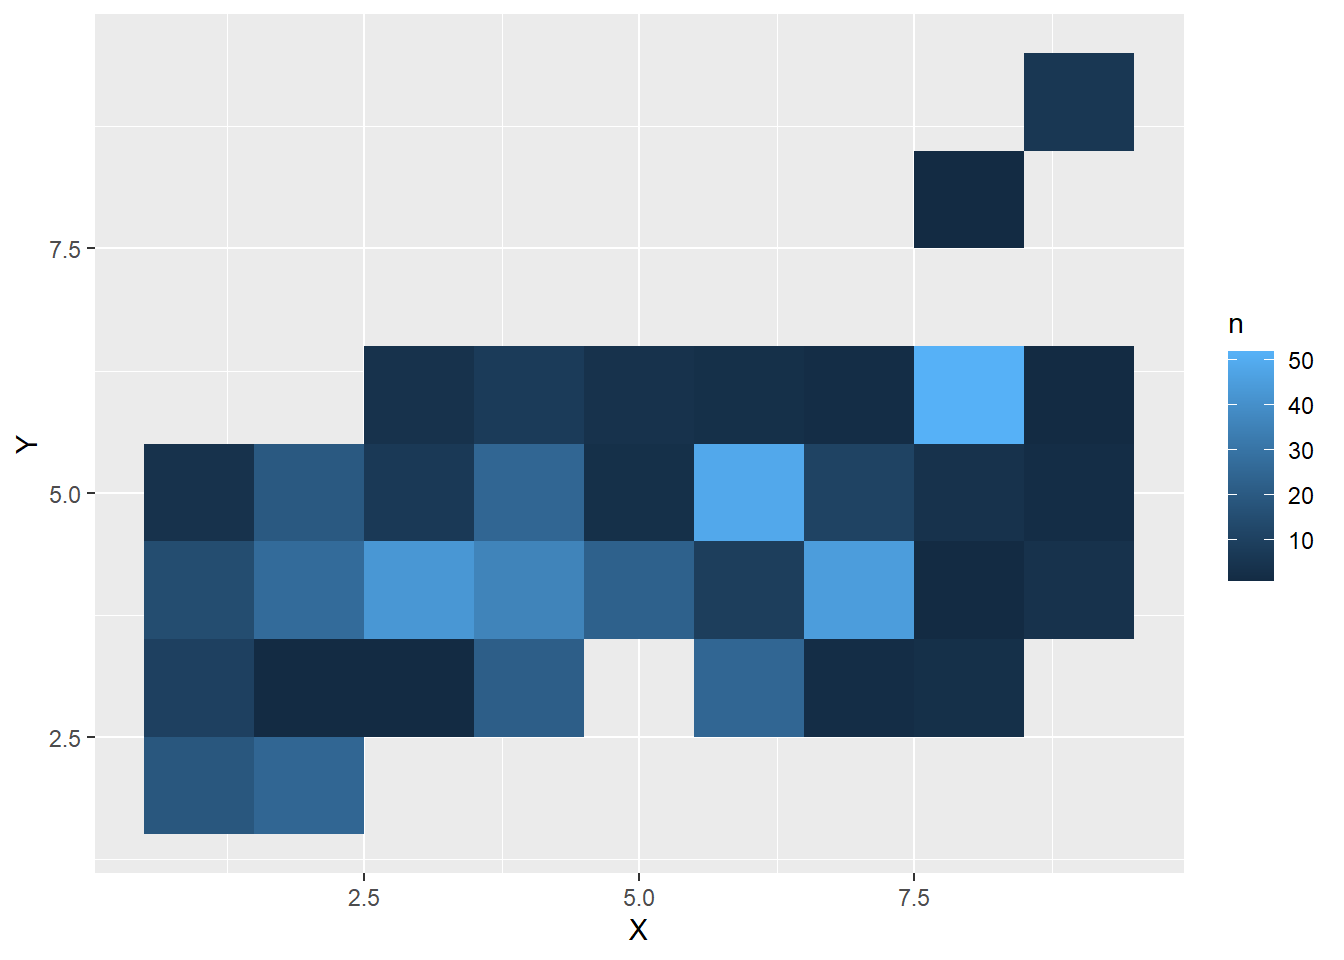
\includegraphics{bookdown-demo_files/figure-latex/unnamed-chunk-76-1.pdf}

  \begin{itemize}
  \tightlist
  \item
    Dodajte stolpec, ki bo za vsak požar izračunal delež požganega območja glede na vse požare na posameznih koordinatah. Za tem smiselno filtrirajte podatke (ali smo v novem stolpcu dobili kakšne nepričakovane, oziroma neveljavne vrednosti?).
  \end{itemize}

\begin{verbatim}
## # A tibble: 509 x 5
##        X     Y month day   area_by_coord
##    <dbl> <dbl> <chr> <chr>         <dbl>
##  1     7     5 mar   fri               0
##  2     7     4 oct   tue               0
##  3     7     4 oct   sat               0
##  4     8     6 mar   fri               0
##  5     8     6 mar   sun               0
##  6     8     6 aug   sun               0
##  7     8     6 aug   mon               0
##  8     8     6 aug   mon               0
##  9     8     6 sep   tue               0
## 10     7     5 sep   sat               0
## # ... with 499 more rows
\end{verbatim}

  \begin{itemize}
  \tightlist
  \item
    Preverite, ali ob vročem vremenu in nizki vlažnosti pogori večji delež območja, ki smo ga izračunali v prejšnji točki, tako da izberete vrstice, kjer je temperatura višja od 0.8 kvantila temperature in vlažnost nižja od 0.2 kvantila vlažnosti ter izračunate povprečje. \(q\)-ti kvantil je ocena števila, za katerega velja, da je \(q\) vrednosti manjših od tega števila. Za računanje kvantilov uporabite funkcijo \texttt{quantile()}. Za primerjavo izračunajte še povprečje te spremenljivke za vse preostale vrstice. Ali se rezultati skladajo z vašo intuicijo?
  \end{itemize}

\begin{verbatim}
## # A tibble: 1 x 1
##   mean_area_by_coord
##                <dbl>
## 1              0.153
\end{verbatim}

\begin{verbatim}
## # A tibble: 1 x 1
##   mean_area_by_coord
##                <dbl>
## 1             0.0555
\end{verbatim}

  \begin{itemize}
  \tightlist
  \item
    Izračunajte povprečje standardiziranih indeksov in ga vstavite kot stolpec pred prvo spremenljivko, ki predstavlja indeks.
  \end{itemize}

\begin{verbatim}
## # A tibble: 509 x 15
## # Rowwise: 
##        X     Y month day   mean_indices FFMC_index DMC_index DC_index ISI_index
##    <dbl> <dbl> <chr> <chr>        <dbl>      <dbl>     <dbl>    <dbl>     <dbl>
##  1     7     5 mar   fri        -1.21     -0.796      -1.32    -1.86   -0.859  
##  2     7     4 oct   tue        -0.304    -0.00502    -1.18     0.480  -0.510  
##  3     7     4 oct   sat        -0.254    -0.00502    -1.05     0.552  -0.510  
##  4     8     6 mar   fri        -0.739     0.193      -1.21    -1.92   -0.00890
##  5     8     6 mar   sun        -0.719    -0.239      -0.934   -1.82    0.122  
##  6     8     6 aug   sun         0.218     0.301      -0.405   -0.256   1.23   
##  7     8     6 aug   mon        -0.0979    0.301      -0.349   -0.225  -0.118  
##  8     8     6 aug   mon         0.320     0.157       0.530    0.232   0.361  
##  9     8     6 sep   tue         0.120     0.0669      0.283    0.575  -0.445  
## 10     7     5 sep   sat         0.0375    0.337      -0.363    0.599  -0.423  
## # ... with 499 more rows, and 6 more variables: temp <dbl>, RH <dbl>,
## #   wind <dbl>, rain <dbl>, area <dbl>, area_by_coord <dbl>
\end{verbatim}
\end{enumerate}

\hypertarget{urejeni-in-relacijski-podatki}{%
\chapter{Urejeni in relacijski podatki}\label{urejeni-in-relacijski-podatki}}

Pri kakršnemkoli delu smo običajno zelo ciljno naravnani. Dobimo nalogo in jo želimo čimprej in čimbolje opraviti. Z namenom učinkovitosti se običajno poslužimo znanih orodij in postopkov, ki jih prilagodimo samemu problemu. Pri delu s podatki se ciljna naravnanost običajno izrazi tako, da želimo čimprej priti do analize in zaključkov, samemu urejanju podatkov pa ne posvetimo pretirane pozornosti, oziroma le toliko, kot je nujno potrebno (kar je še vedno lahko dolgotrajno). Na kratek rok to deluje v redu in celo prihranimo nekaj časa. Na dolgi rok pa običajno zahteva veliko več časa, saj se moramo pri vsaki novi nalogi na novo prilagajati podatkom. Boljši pristop bi bil, da bi problem prilagodili ustaljenemu postopku. Običajno lahko večino podatkov uredimo do te mere, da so si po obliki podobni. V kolikor se naučimo narediti to za neko splošno podatkovno zbirko, lahko potem vsakič pristopimo do nadaljnjega dela na podoben način. V praksi s tem na dolgi rok prihranimo veliko časa.

Koncept \textbf{urejenih podatkov} (ang. \textbf{tidy data}), ki ga bomo spoznali v tem poglavju, je formalizacija intuitivne predstavke kaj podatki so. Podatke, ki so \textbf{urejeni}, lahko veliko lažje transformiramo in pripravimo na nadaljnjo analizo. Tudi funkcije v tidyverse so implementirane tako, da na vhod prejmejo urejene podatke in takšne tudi vrnejo. Z drugimi besedami ohranjajo urejenost.

Relacijski podatki pa so podatki o različnih entitetah (na primer podjetje, delavec, službeno vozilo, klient), ki so shranjeni v različnih razpredelnicah. Kadar želimo analizirati relacijske podatke moramo razumeti povezave med njimi in kako delati z njimi. Spoznali bomo koncept relacijskih podatkovnih zbirk in kako uporabiti tidyverse za delo z njimi.

\hypertarget{priprava-1}{%
\section{Priprava}\label{priprava-1}}

V tem poglavju bomo spoznali, kako podatke pretvorimo iz daljše v krajšo obliko (in obratno) ter kako delamo z relacijskimi podatki. Kaj vsi ti koncepti pomenijo in kako so povezani z urejenimi podatki, bomo predelali v jedru poglavja.

Pri pretvorbi podatkov v daljšo obliko gre za pretvorbo, kjer vrednosti večih stolpcev združimo v en stolpec. Poglejmo si razpredelnico, kjer imamo shranjene podatke za več let:

\begin{Shaded}
\begin{Highlighting}[]
\NormalTok{df }\OtherTok{\textless{}{-}} \FunctionTok{tibble}\NormalTok{(}
  \AttributeTok{ime =} \FunctionTok{c}\NormalTok{(}\StringTok{"Mojca"}\NormalTok{, }\StringTok{"Miha"}\NormalTok{, }\StringTok{"Mateja"}\NormalTok{),}
  \StringTok{\textasciigrave{}}\AttributeTok{2018}\StringTok{\textasciigrave{}} \OtherTok{=} \FunctionTok{c}\NormalTok{(}\FloatTok{5.5}\NormalTok{, }\FloatTok{4.6}\NormalTok{, }\FloatTok{8.7}\NormalTok{),}
  \StringTok{\textasciigrave{}}\AttributeTok{2019}\StringTok{\textasciigrave{}} \OtherTok{=} \FunctionTok{c}\NormalTok{(}\FloatTok{5.8}\NormalTok{, }\FloatTok{4.2}\NormalTok{, }\DecValTok{9}\NormalTok{)}
\NormalTok{)}
\NormalTok{df}
\end{Highlighting}
\end{Shaded}

\begin{verbatim}
## # A tibble: 3 x 3
##   ime    `2018` `2019`
##   <chr>   <dbl>  <dbl>
## 1 Mojca     5.5    5.8
## 2 Miha      4.6    4.2
## 3 Mateja    8.7    9
\end{verbatim}

Recimo, da želimo stolpca z leti spraviti v en stolpec. Uporabimo funkcijo \texttt{pivot\_longer()}.

\begin{Shaded}
\begin{Highlighting}[]
\NormalTok{df\_longer }\OtherTok{\textless{}{-}} \FunctionTok{pivot\_longer}\NormalTok{(df, }\FunctionTok{c}\NormalTok{(}\StringTok{\textasciigrave{}}\AttributeTok{2018}\StringTok{\textasciigrave{}}\NormalTok{, }\StringTok{\textasciigrave{}}\AttributeTok{2019}\StringTok{\textasciigrave{}}\NormalTok{), }\AttributeTok{names\_to =} \StringTok{"leto"}\NormalTok{, }\AttributeTok{values\_to =} \StringTok{"rezultat"}\NormalTok{)}
\NormalTok{df\_longer}
\end{Highlighting}
\end{Shaded}

\begin{verbatim}
## # A tibble: 6 x 3
##   ime    leto  rezultat
##   <chr>  <chr>    <dbl>
## 1 Mojca  2018       5.5
## 2 Mojca  2019       5.8
## 3 Miha   2018       4.6
## 4 Miha   2019       4.2
## 5 Mateja 2018       8.7
## 6 Mateja 2019       9
\end{verbatim}

Lahko naredimo tudi obratno transformacijo, torej da vrednosti enega stolpca razširimo v več stolpcev. Na primer, razširimo stolpec \texttt{ime}:

\begin{Shaded}
\begin{Highlighting}[]
\FunctionTok{pivot\_wider}\NormalTok{(df\_longer, }\AttributeTok{names\_from =}\NormalTok{ ime, }\AttributeTok{values\_from =}\NormalTok{ rezultat)}
\end{Highlighting}
\end{Shaded}

\begin{verbatim}
## # A tibble: 2 x 4
##   leto  Mojca  Miha Mateja
##   <chr> <dbl> <dbl>  <dbl>
## 1 2018    5.5   4.6    8.7
## 2 2019    5.8   4.2    9
\end{verbatim}

\textbf{Naloga}: Spodnjo razpredelnico transformirajte v daljšo obliko, tako da informacije o številu oddelkov shranite v 1 stolpec.

\begin{Shaded}
\begin{Highlighting}[]
\NormalTok{df }\OtherTok{\textless{}{-}} \FunctionTok{tibble}\NormalTok{(}
  \AttributeTok{podjetje =} \FunctionTok{c}\NormalTok{(}\StringTok{"Podjetje A"}\NormalTok{, }\StringTok{"Podjetje A"}\NormalTok{, }\StringTok{"Podjetje B"}\NormalTok{),}
  \AttributeTok{kraj\_tovarne =} \FunctionTok{c}\NormalTok{(}\StringTok{"Koper"}\NormalTok{, }\StringTok{"Kranj"}\NormalTok{, }\StringTok{"Koper"}\NormalTok{),}
  \AttributeTok{prihodek =} \FunctionTok{c}\NormalTok{(}\DecValTok{100000}\NormalTok{, }\DecValTok{120000}\NormalTok{, }\DecValTok{60000}\NormalTok{),}
  \AttributeTok{razvojni\_oddelki =} \FunctionTok{c}\NormalTok{(}\DecValTok{2}\NormalTok{, }\DecValTok{3}\NormalTok{, }\DecValTok{1}\NormalTok{),}
  \AttributeTok{prodajni\_oddelki =} \FunctionTok{c}\NormalTok{(}\DecValTok{3}\NormalTok{, }\DecValTok{3}\NormalTok{, }\DecValTok{2}\NormalTok{)}
\NormalTok{)}
\NormalTok{df}
\end{Highlighting}
\end{Shaded}

\begin{verbatim}
## # A tibble: 3 x 5
##   podjetje   kraj_tovarne prihodek razvojni_oddelki prodajni_oddelki
##   <chr>      <chr>           <dbl>            <dbl>            <dbl>
## 1 Podjetje A Koper          100000                2                3
## 2 Podjetje A Kranj          120000                3                3
## 3 Podjetje B Koper           60000                1                2
\end{verbatim}

Rešitev:

\begin{verbatim}
## # A tibble: 6 x 5
##   podjetje   kraj_tovarne prihodek oddelek          stevilo_oddelkov
##   <chr>      <chr>           <dbl> <chr>                       <dbl>
## 1 Podjetje A Koper          100000 razvojni_oddelki                2
## 2 Podjetje A Koper          100000 prodajni_oddelki                3
## 3 Podjetje A Kranj          120000 razvojni_oddelki                3
## 4 Podjetje A Kranj          120000 prodajni_oddelki                3
## 5 Podjetje B Koper           60000 razvojni_oddelki                1
## 6 Podjetje B Koper           60000 prodajni_oddelki                2
\end{verbatim}

Spoznali bomo tudi relacijske podatke, pri katerih so podatki razdeljeni med več razpredelnic. Zato bomo potrebovali več funkcij, ki nam omogočajo združevanje teh razpredelnic. Poglejmo si dve razpredelnici:

\begin{Shaded}
\begin{Highlighting}[]
\NormalTok{ekipe }\OtherTok{\textless{}{-}} \FunctionTok{tibble}\NormalTok{(}
  \AttributeTok{id\_ekipe =} \FunctionTok{c}\NormalTok{(}\DecValTok{1}\NormalTok{, }\DecValTok{2}\NormalTok{, }\DecValTok{3}\NormalTok{, }\DecValTok{4}\NormalTok{),}
  \AttributeTok{ekipa =} \FunctionTok{c}\NormalTok{(}\StringTok{"Liverpool"}\NormalTok{, }\StringTok{"Manchester United"}\NormalTok{, }\StringTok{"Arsenal"}\NormalTok{, }\StringTok{"Rokova ekipa"}\NormalTok{)}
\NormalTok{)}
\NormalTok{igralci }\OtherTok{\textless{}{-}} \FunctionTok{tibble}\NormalTok{(}
  \AttributeTok{id\_igralca =} \FunctionTok{c}\NormalTok{(}\DecValTok{1}\NormalTok{, }\DecValTok{2}\NormalTok{, }\DecValTok{3}\NormalTok{, }\DecValTok{4}\NormalTok{, }\DecValTok{5}\NormalTok{, }\DecValTok{6}\NormalTok{, }\DecValTok{7}\NormalTok{),}
  \AttributeTok{ime =} \FunctionTok{c}\NormalTok{(}\StringTok{"Henderson"}\NormalTok{, }\StringTok{"Fernandes"}\NormalTok{, }\StringTok{"Alisson"}\NormalTok{, }\StringTok{"Rashford"}\NormalTok{, }\StringTok{"Novak"}\NormalTok{, }\StringTok{"Aubameyang"}\NormalTok{, }\StringTok{"Vega"}\NormalTok{),}
  \AttributeTok{id\_ekipe =} \FunctionTok{c}\NormalTok{(}\DecValTok{1}\NormalTok{, }\DecValTok{2}\NormalTok{, }\DecValTok{1}\NormalTok{, }\DecValTok{2}\NormalTok{, }\DecValTok{8}\NormalTok{, }\DecValTok{3}\NormalTok{, }\DecValTok{8}\NormalTok{)}
\NormalTok{)}
\NormalTok{ekipe}
\end{Highlighting}
\end{Shaded}

\begin{verbatim}
## # A tibble: 4 x 2
##   id_ekipe ekipa            
##      <dbl> <chr>            
## 1        1 Liverpool        
## 2        2 Manchester United
## 3        3 Arsenal          
## 4        4 Rokova ekipa
\end{verbatim}

\begin{Shaded}
\begin{Highlighting}[]
\NormalTok{igralci}
\end{Highlighting}
\end{Shaded}

\begin{verbatim}
## # A tibble: 7 x 3
##   id_igralca ime        id_ekipe
##        <dbl> <chr>         <dbl>
## 1          1 Henderson         1
## 2          2 Fernandes         2
## 3          3 Alisson           1
## 4          4 Rashford          2
## 5          5 Novak             8
## 6          6 Aubameyang        3
## 7          7 Vega              8
\end{verbatim}

Za združevanje razpredelnic obstaja več funkcij, vse imajo končnico \texttt{\_join}. Poglejmo si, kako jih kličemo in kaj vsaka izmed njih naredi. Več bomo o njih povedali na predavanju.

\texttt{left\_join()} združi razpredelnici tako, da obdrži vse primere iz prve razpredelnice:

\begin{Shaded}
\begin{Highlighting}[]
\FunctionTok{left\_join}\NormalTok{(igralci, ekipe, }\AttributeTok{by =} \StringTok{"id\_ekipe"}\NormalTok{)}
\end{Highlighting}
\end{Shaded}

\begin{verbatim}
## # A tibble: 7 x 4
##   id_igralca ime        id_ekipe ekipa            
##        <dbl> <chr>         <dbl> <chr>            
## 1          1 Henderson         1 Liverpool        
## 2          2 Fernandes         2 Manchester United
## 3          3 Alisson           1 Liverpool        
## 4          4 Rashford          2 Manchester United
## 5          5 Novak             8 <NA>             
## 6          6 Aubameyang        3 Arsenal          
## 7          7 Vega              8 <NA>
\end{verbatim}

\texttt{right\_join()} združi razpredelnici tako, da obdrži vse primere iz druge razpredelnice:

\begin{Shaded}
\begin{Highlighting}[]
\FunctionTok{right\_join}\NormalTok{(igralci, ekipe, }\AttributeTok{by =} \StringTok{"id\_ekipe"}\NormalTok{)}
\end{Highlighting}
\end{Shaded}

\begin{verbatim}
## # A tibble: 6 x 4
##   id_igralca ime        id_ekipe ekipa            
##        <dbl> <chr>         <dbl> <chr>            
## 1          1 Henderson         1 Liverpool        
## 2          2 Fernandes         2 Manchester United
## 3          3 Alisson           1 Liverpool        
## 4          4 Rashford          2 Manchester United
## 5          6 Aubameyang        3 Arsenal          
## 6         NA <NA>              4 Rokova ekipa
\end{verbatim}

\texttt{inner\_join()} združi razpredelnici tako, da obdrži samo primere, ki se pojavijo v obeh razpredelnicah:

\begin{Shaded}
\begin{Highlighting}[]
\FunctionTok{inner\_join}\NormalTok{(igralci, ekipe, }\AttributeTok{by =} \StringTok{"id\_ekipe"}\NormalTok{)}
\end{Highlighting}
\end{Shaded}

\begin{verbatim}
## # A tibble: 5 x 4
##   id_igralca ime        id_ekipe ekipa            
##        <dbl> <chr>         <dbl> <chr>            
## 1          1 Henderson         1 Liverpool        
## 2          2 Fernandes         2 Manchester United
## 3          3 Alisson           1 Liverpool        
## 4          4 Rashford          2 Manchester United
## 5          6 Aubameyang        3 Arsenal
\end{verbatim}

\texttt{full\_join()} združi razpredelnici tako, da obdrži vse primere iz obeh razpredelnic:

\begin{Shaded}
\begin{Highlighting}[]
\FunctionTok{full\_join}\NormalTok{(igralci, ekipe, }\AttributeTok{by =} \StringTok{"id\_ekipe"}\NormalTok{)}
\end{Highlighting}
\end{Shaded}

\begin{verbatim}
## # A tibble: 8 x 4
##   id_igralca ime        id_ekipe ekipa            
##        <dbl> <chr>         <dbl> <chr>            
## 1          1 Henderson         1 Liverpool        
## 2          2 Fernandes         2 Manchester United
## 3          3 Alisson           1 Liverpool        
## 4          4 Rashford          2 Manchester United
## 5          5 Novak             8 <NA>             
## 6          6 Aubameyang        3 Arsenal          
## 7          7 Vega              8 <NA>             
## 8         NA <NA>              4 Rokova ekipa
\end{verbatim}

\textbf{Naloga}: Obstajata še dve operaciji združevanja, ki pa ne delujeta popolnoma enako kot zgornje funkcije. Pokličite funkciji \texttt{semi\_join()} in \texttt{anti\_join()} in poizkusite ugotoviti, kaj sta ti funkciji naredili. Sintaksa je enaka kot pri ostalih funkcijah join.

Za branje podatkov iz tekstovnih datotek velikokrat uporabljamo funkcijo \texttt{read.csv()} ali katero od preostalih izpeljank funkcije \texttt{read.table()}. Tidyverse ima svojo različico teh funkcij, ki pa imajo nekaj dodatne funkcionalnosti. Najbolj pomembna je ta, da se podatki samodejno shranijo kot tibble. To omogoča relativno enostavno branje datotek, kjer stolpci niso poimenovani v skladu s pravili programskega jezika R (na primer, lahko se začnejo s številom, lahko imajo minuse, presledke in podobno). Kot smo omenili shranjevanje podatkov, kjer imena stolpcev niso standardne oblike, ni dobra praksa. Vsekakor pa se pri realnih podatkih velikokrat zgodi, da imamo takšna imena. V tem primeru je bolje, da jih prebermo takšna kot so in jih programsko spremenimo, saj s tem ne posegamo v izvirne podatke. Je pa potrebno pri teh funkcijah dodatno nastaviti kodiranje, da znajo prebrati šumnike. Poglejmo si uporabo funkcije \texttt{read\_csv2()} paketa \texttt{readr}, kjer bomo ustrezno nastavili kodiranje.

\begin{Shaded}
\begin{Highlighting}[]
\NormalTok{df }\OtherTok{\textless{}{-}} \FunctionTok{read\_csv2}\NormalTok{(}\StringTok{"./data{-}raw/SLO{-}gradbena{-}dovoljenja{-}messy1.csv"}\NormalTok{,}
                \AttributeTok{locale =}\NormalTok{ readr}\SpecialCharTok{::}\FunctionTok{locale}\NormalTok{(}\AttributeTok{encoding =} \StringTok{"cp1250"}\NormalTok{))}
\end{Highlighting}
\end{Shaded}

Več o kodiranjih bomo povedali na zadnjem predavanju.

\hypertarget{urejeni-podatki}{%
\section{Urejeni podatki}\label{urejeni-podatki}}

Omenili smo že, da se v praksi srečamo z najrazličnejšimi oblikami zapisov podatkov. Skupek paketov tidyverse je namenjen delu s tako imenovanimi \textbf{urejenimi podatki} (ang. \textbf{tidy data}). Ideja je, da se ustvari enoten standard za obliko podatkov, s katero je lažje delati. V kolikor se držimo tega standarda pri vseh naših analizah, nam to omogoča, da vedno uporabljamo ista orodja (na primer, ggplot2) in se nam ni potrebno učiti novih orodij za vsako analizo. Standard lahko povzamemo s 3 lastnostmi:

\begin{enumerate}
\def\labelenumi{\arabic{enumi})}
\tightlist
\item
  vsak stolpec je spremenljivka,
\item
  vsaka vrstica je primer podatka,
\item
  vsaka vrednost ima svojo celico.
\end{enumerate}

Morda se na tej točki to sliši nekoliko abstraktno. Poglejmo si praktičen primer. Nabrali smo podatke o številu izdanih gradbenih dovoljenj v Sloveniji, razdeljeno glede na občine. Podatke smo prenesli s spletne strani statističnega urada Slovenije \url{https://pxweb.stat.si/SiStat/slshranili} in jih shranili na več načinov. Najprej si poglejmo podatke v takšni obliki, kot smo jih dobili naravnost iz vira.

\begin{verbatim}
## # A tibble: 424 x 16
##    OBČINE   TIP.STAVBE   `2007` `2008` `2009` `2010` `2011` `2012` `2013` `2014`
##    <chr>    <chr>         <dbl>  <dbl>  <dbl>  <dbl>  <dbl>  <dbl>  <dbl>  <dbl>
##  1 Ajdovšč~ Stanovanjsk~     52     55     45     33     52     40     29     30
##  2 Ajdovšč~ Nestanovanj~     19      9     22     15     27     11     23     11
##  3 Ankaran~ Stanovanjsk~     NA     NA     NA     NA     NA     NA     NA     NA
##  4 Ankaran~ Nestanovanj~     NA     NA     NA     NA     NA     NA     NA     NA
##  5 Apače    Stanovanjsk~     10     11     22     12      7      5      9     10
##  6 Apače    Nestanovanj~      3      3      8      3      4      6      2      3
##  7 Beltinci Stanovanjsk~     16     19     11     15     19     14      5     13
##  8 Beltinci Nestanovanj~      4      6      1      3      8      4      4      5
##  9 Benedikt Stanovanjsk~     11     12      6      9      7      3     16     10
## 10 Benedikt Nestanovanj~      3      2      1      3      5      3      4      3
## # ... with 414 more rows, and 6 more variables: 2015 <dbl>, 2016 <dbl>,
## #   2017 <dbl>, 2018 <dbl>, 2019 <dbl>, 2020 <dbl>
\end{verbatim}

Najprej imamo na voljo spremenljivki \texttt{OBČINE} in \texttt{TIP.STAVBE}. Potem pa imamo za vsako leto naštete vrednosti, oziroma števila gradbenih dovoljenj. Podatki so velikokrat shranjeni v takšnem formatu, saj ima določene prednosti. Tak format je bolj prijazen za prikaz človeku, saj lahko samo s pogledom na razpredelnico hitro oceni, ali obstaja trend v posamezni vrstici. Format pa ni najboljši za delo s podatki. Govorili smo že o čistih podatkih in da vse funkcije v tidyverse podpirajo operacije nad takšnimi podatki. Kot vhod bo večina teh funkcij prejela čiste podatke in takšne potem tudi vrnila.

Kaj je razlog, da ti podatki niso čisti? Ne drži, da imamo v vsakem stolpcu spremenljivko, saj imamo eno spremenljivko razvlečeno čez več stolpcev -- leto. Ta podatek vsekakor predstavlja spremenljivko, torej bi moral imeti enoten stolpec. Poglejmo si te podatke še v dveh nečistih formatih.

\begin{verbatim}
## # A tibble: 28 x 214
##    TIP.STAVBE          Leto Ajdovščina `Ankaran/Ancaran~ Apače Beltinci Benedikt
##    <chr>              <dbl>      <dbl>             <dbl> <dbl>    <dbl>    <dbl>
##  1 Stanovanjske stav~  2007         52                NA    10       16       11
##  2 Stanovanjske stav~  2008         55                NA    11       19       12
##  3 Stanovanjske stav~  2009         45                NA    22       11        6
##  4 Stanovanjske stav~  2010         33                NA    12       15        9
##  5 Stanovanjske stav~  2011         52                NA     7       19        7
##  6 Stanovanjske stav~  2012         40                NA     5       14        3
##  7 Stanovanjske stav~  2013         29                NA     9        5       16
##  8 Stanovanjske stav~  2014         30                NA    10       13       10
##  9 Stanovanjske stav~  2015         38                 3    12       23       13
## 10 Stanovanjske stav~  2016         31                 1    10       22       15
## # ... with 18 more rows, and 207 more variables: Bistrica ob Sotli <dbl>,
## #   Bled <dbl>, Bloke <dbl>, Bohinj <dbl>, Borovnica <dbl>, Bovec <dbl>,
## #   Braslovče <dbl>, Brda <dbl>, Brezovica <dbl>, Brežice <dbl>, Cankova <dbl>,
## #   Celje <dbl>, Cerklje na Gorenjskem <dbl>, Cerknica <dbl>, Cerkno <dbl>,
## #   Cerkvenjak <dbl>, Cirkulane <dbl>, Črenšovci <dbl>, Črna na Koroškem <dbl>,
## #   Črnomelj <dbl>, Destrnik <dbl>, Divača <dbl>, Dobje <dbl>,
## #   Dobrepolje <dbl>, Dobrna <dbl>, Dobrova - Polhov Gradec <dbl>,
## #   Dobrovnik/Dobronak <dbl>, Dol pri Ljubljani <dbl>, Dolenjske Toplice <dbl>,
## #   Domžale <dbl>, Dornava <dbl>, Dravograd <dbl>, Duplek <dbl>,
## #   Gorenja vas - Poljane <dbl>, Gorišnica <dbl>, Gorje <dbl>,
## #   Gornja Radgona <dbl>, Gornji Grad <dbl>, Gornji Petrovci <dbl>, Grad <dbl>,
## #   Grosuplje <dbl>, Hajdina <dbl>, Hoče - Slivnica <dbl>, Hodoš/Hodos <dbl>,
## #   Horjul <dbl>, Hrastnik <dbl>, Hrpelje - Kozina <dbl>, Idrija <dbl>,
## #   Ig <dbl>, Ilirska Bistrica <dbl>, Ivančna Gorica <dbl>, Izola/Isola <dbl>,
## #   Jesenice <dbl>, Jezersko <dbl>, Juršinci <dbl>, Kamnik <dbl>, Kanal <dbl>,
## #   Kidričevo <dbl>, Kobarid <dbl>, Kobilje <dbl>, Kočevje <dbl>, Komen <dbl>,
## #   Komenda <dbl>, Koper/Capodistria <dbl>, Kostanjevica na Krki <dbl>,
## #   Kostel <dbl>, Kozje <dbl>, Kranj <dbl>, Kranjska Gora <dbl>,
## #   Križevci <dbl>, Krško <dbl>, Kungota <dbl>, Kuzma <dbl>, Laško <dbl>,
## #   Lenart <dbl>, Lendava/Lendva <dbl>, Litija <dbl>, Ljubljana <dbl>,
## #   Ljubno <dbl>, Ljutomer <dbl>, Log - Dragomer <dbl>, Logatec <dbl>,
## #   Loška dolina <dbl>, Loški Potok <dbl>, Lovrenc na Pohorju <dbl>,
## #   Luče <dbl>, Lukovica <dbl>, Majšperk <dbl>, Makole <dbl>, Maribor <dbl>,
## #   Markovci <dbl>, Medvode <dbl>, Mengeš <dbl>, Metlika <dbl>, Mežica <dbl>,
## #   Miklavž na Dravskem polju <dbl>, Miren - Kostanjevica <dbl>, Mirna <dbl>,
## #   Mirna Peč <dbl>, Mislinja <dbl>, ...
\end{verbatim}

Sedaj imamo podobno situacijo kot prej -- ena spremenljivka je razvlečena preko več stolpcev -- v tem primeru je to občina. Kot smo že omenili, so vsaki nečisti podatki nečisti na svoj način. Podatki so popolnoma enaki kot v prejšnjem prikazu, ampak razpredelnica izgleda popolnoma drugače. Čisti podatki pa imajo samo eno pravilno obliko, torej ne more priti do takšnih dvoumnih prikazov.

Poglejmo si še tretji format:

\begin{verbatim}
## # A tibble: 5,936 x 3
##    OBČINA_TIP                      Leto Število.gradbenih.dovoljenj
##    <chr>                          <dbl>                       <dbl>
##  1 Ajdovščina_Stanovanjske stavbe  2007                          52
##  2 Ajdovščina_Stanovanjske stavbe  2008                          55
##  3 Ajdovščina_Stanovanjske stavbe  2009                          45
##  4 Ajdovščina_Stanovanjske stavbe  2010                          33
##  5 Ajdovščina_Stanovanjske stavbe  2011                          52
##  6 Ajdovščina_Stanovanjske stavbe  2012                          40
##  7 Ajdovščina_Stanovanjske stavbe  2013                          29
##  8 Ajdovščina_Stanovanjske stavbe  2014                          30
##  9 Ajdovščina_Stanovanjske stavbe  2015                          38
## 10 Ajdovščina_Stanovanjske stavbe  2016                          31
## # ... with 5,926 more rows
\end{verbatim}

Ta je morda nekoliko bližje čistim podatkom, kot prejšnja dva, ampak še vedno ni v popolnoma pravilni obliki. V čem je težava? Dve spremenljivki imamo podani v enem stolpcu -- občino in tip. Ker gre za različni spremenljivki, bi bilo dobro, da se pojavita v različnih stolpcih.

Poglejmo si sedaj še čiste podatke:

\begin{verbatim}
## # A tibble: 5,936 x 4
##    OBČINE     TIP.STAVBE           Leto Število.gradbenih.dovoljenj
##    <chr>      <chr>               <dbl>                       <dbl>
##  1 Ajdovščina Stanovanjske stavbe  2007                          52
##  2 Ajdovščina Stanovanjske stavbe  2008                          55
##  3 Ajdovščina Stanovanjske stavbe  2009                          45
##  4 Ajdovščina Stanovanjske stavbe  2010                          33
##  5 Ajdovščina Stanovanjske stavbe  2011                          52
##  6 Ajdovščina Stanovanjske stavbe  2012                          40
##  7 Ajdovščina Stanovanjske stavbe  2013                          29
##  8 Ajdovščina Stanovanjske stavbe  2014                          30
##  9 Ajdovščina Stanovanjske stavbe  2015                          38
## 10 Ajdovščina Stanovanjske stavbe  2016                          31
## # ... with 5,926 more rows
\end{verbatim}

Sedaj ima vsaka spremenljivka (občina, tip in leto) svoj stolpec, zadnji stolpec pa je namenjen vrednostim. V tem poglavju se bomo naučili nečiste podatke spremeniti v čiste.

Čisti podatki imajo običajno več vrstic kot nečisti in jim zato pravimo da so \textbf{daljši} (ang. \textbf{longer}). Nečisti pa so običajno \textbf{širši} (ang. \textbf{wider}). Izogibamo se besedam dolgi in široki, saj je ta definicija relativna, se pravi lahko uporabimo transformacijo, ki naredi podatke daljše, ne pa nujno dolge, saj morda obstaja še kakšna operacija, ki jih bo naredila še daljše.

\hypertarget{pivot_longer-pretvorba-v-daljux161o-obliko}{%
\section{\texorpdfstring{\texttt{pivot\_longer()}: pretvorba v daljšo obliko}{pivot\_longer(): pretvorba v daljšo obliko}}\label{pivot_longer-pretvorba-v-daljux161o-obliko}}

Funkcija \texttt{pivot\_longer()} podatke spremeni v daljšo obliko. Ta trasformacija je pri delu s podatki bolj pogosta kot sprememba v širšo. Običajno uporabljamo to transformacijo, ko preurejamo podatke v čiste.

Poglejmo si ponovno nečiste podatke, ki smo jih dobili naravnost iz vira:

\begin{verbatim}
## # A tibble: 424 x 16
##    OBČINE   TIP.STAVBE   `2007` `2008` `2009` `2010` `2011` `2012` `2013` `2014`
##    <chr>    <chr>         <dbl>  <dbl>  <dbl>  <dbl>  <dbl>  <dbl>  <dbl>  <dbl>
##  1 Ajdovšč~ Stanovanjsk~     52     55     45     33     52     40     29     30
##  2 Ajdovšč~ Nestanovanj~     19      9     22     15     27     11     23     11
##  3 Ankaran~ Stanovanjsk~     NA     NA     NA     NA     NA     NA     NA     NA
##  4 Ankaran~ Nestanovanj~     NA     NA     NA     NA     NA     NA     NA     NA
##  5 Apače    Stanovanjsk~     10     11     22     12      7      5      9     10
##  6 Apače    Nestanovanj~      3      3      8      3      4      6      2      3
##  7 Beltinci Stanovanjsk~     16     19     11     15     19     14      5     13
##  8 Beltinci Nestanovanj~      4      6      1      3      8      4      4      5
##  9 Benedikt Stanovanjsk~     11     12      6      9      7      3     16     10
## 10 Benedikt Nestanovanj~      3      2      1      3      5      3      4      3
## # ... with 414 more rows, and 6 more variables: 2015 <dbl>, 2016 <dbl>,
## #   2017 <dbl>, 2018 <dbl>, 2019 <dbl>, 2020 <dbl>
\end{verbatim}

Sedaj želimo te podatke spremeniti v čisto obliko. Vse stolpce, ki prikazujejo različne vrednosti spremenljivke leto, moramo zapisati v 1 stolpec. Uporabimo funkcijo \texttt{pivot\_longer()}, ki prejme argumente:

\begin{itemize}
\tightlist
\item
  \texttt{data}. Katere podatke želimo spremeniti.
\item
  \texttt{cols}. V katerih stolpcih imamo vrednosti spremenljivke, ki jo želimo shraniti v 1 stolpec.
\end{itemize}

\begin{Shaded}
\begin{Highlighting}[]
\NormalTok{df }\SpecialCharTok{\%\textgreater{}\%} \FunctionTok{pivot\_longer}\NormalTok{(}\AttributeTok{cols =} \StringTok{\textasciigrave{}}\AttributeTok{2007}\StringTok{\textasciigrave{}}\SpecialCharTok{:}\StringTok{\textasciigrave{}}\AttributeTok{2020}\StringTok{\textasciigrave{}}\NormalTok{)}
\end{Highlighting}
\end{Shaded}

\begin{verbatim}
## # A tibble: 5,936 x 4
##    OBČINE     TIP.STAVBE          name  value
##    <chr>      <chr>               <chr> <dbl>
##  1 Ajdovščina Stanovanjske stavbe 2007     52
##  2 Ajdovščina Stanovanjske stavbe 2008     55
##  3 Ajdovščina Stanovanjske stavbe 2009     45
##  4 Ajdovščina Stanovanjske stavbe 2010     33
##  5 Ajdovščina Stanovanjske stavbe 2011     52
##  6 Ajdovščina Stanovanjske stavbe 2012     40
##  7 Ajdovščina Stanovanjske stavbe 2013     29
##  8 Ajdovščina Stanovanjske stavbe 2014     30
##  9 Ajdovščina Stanovanjske stavbe 2015     38
## 10 Ajdovščina Stanovanjske stavbe 2016     31
## # ... with 5,926 more rows
\end{verbatim}

Sedaj imamo leta shranjena v stolpcu, prav tako pa vrednosti. Stolpca sta dobila privzeti meni \texttt{name} in \texttt{value}. Funkcija \texttt{pivot\_longer()} pa lahko prejme še več opcijskih argumentov, za nas bosta najbolj pomembna 2:

\begin{itemize}
\tightlist
\item
  \texttt{names\_to}. Ime stolpca, v katerega bomo shranili spremenljivko.
\item
  \texttt{value\_to}. Ime stolpca, v katerega bomo shranili vrednosti.
\end{itemize}

Uporabimo sedaj še ta 2 parametra:

\begin{Shaded}
\begin{Highlighting}[]
\NormalTok{df\_longer }\OtherTok{\textless{}{-}}\NormalTok{ df }\SpecialCharTok{\%\textgreater{}\%} \FunctionTok{pivot\_longer}\NormalTok{(}\AttributeTok{cols =} \StringTok{\textasciigrave{}}\AttributeTok{2007}\StringTok{\textasciigrave{}}\SpecialCharTok{:}\StringTok{\textasciigrave{}}\AttributeTok{2020}\StringTok{\textasciigrave{}}\NormalTok{, }
                                 \AttributeTok{names\_to =} \StringTok{"Leto"}\NormalTok{, }
                                 \AttributeTok{values\_to =} \StringTok{"Število"}\NormalTok{)}
\NormalTok{df\_longer}
\end{Highlighting}
\end{Shaded}

\begin{verbatim}
## # A tibble: 5,936 x 4
##    OBČINE     TIP.STAVBE          Leto  Število
##    <chr>      <chr>               <chr>   <dbl>
##  1 Ajdovščina Stanovanjske stavbe 2007       52
##  2 Ajdovščina Stanovanjske stavbe 2008       55
##  3 Ajdovščina Stanovanjske stavbe 2009       45
##  4 Ajdovščina Stanovanjske stavbe 2010       33
##  5 Ajdovščina Stanovanjske stavbe 2011       52
##  6 Ajdovščina Stanovanjske stavbe 2012       40
##  7 Ajdovščina Stanovanjske stavbe 2013       29
##  8 Ajdovščina Stanovanjske stavbe 2014       30
##  9 Ajdovščina Stanovanjske stavbe 2015       38
## 10 Ajdovščina Stanovanjske stavbe 2016       31
## # ... with 5,926 more rows
\end{verbatim}

\hypertarget{pivot_wider-pretvorba-v-ux161irux161o-obliko}{%
\section{\texorpdfstring{\texttt{pivot\_wider()}: pretvorba v širšo obliko}{pivot\_wider(): pretvorba v širšo obliko}}\label{pivot_wider-pretvorba-v-ux161irux161o-obliko}}

Običajno bo ta transformacija naredila podatke nečiste, vendar s tem ni nič narobe, saj imajo tudi takšni podatki svoje prednosti:

\begin{itemize}
\tightlist
\item
  Podatki v širši obliki so človeku lažje berljivi.
\item
  Nekatera podjetja in področja imajo razvite standarde, v katerih potrebujemo podatke v širši obliki.
\item
  Nekatere metode, predvsem gre tukaj za metode strojnega učenja, delujejo bolje ali izključno s podatki v širši obliki.
\item
  Če želimo podatke pretvoriti v matriko.
\end{itemize}

Za pretvorbo podatkov v širšo obliko uporabimo funkcijo \texttt{pivot\_wider()}, ki prejme dva argumenta:

\begin{itemize}
\tightlist
\item
  \texttt{names\_from}. Ime stolpca, katerga želimo raztegniti v širšo obliko.
\item
  \texttt{values\_from}. Ime stolpca, v katerem so shranjene vrednosti.
\end{itemize}

Pretvorimo sedaj \texttt{df\_longer} v širšo obliko glede na stolpec \texttt{TIP.STAVBE}.

\begin{Shaded}
\begin{Highlighting}[]
\NormalTok{df\_wider }\OtherTok{\textless{}{-}}\NormalTok{ df\_longer }\SpecialCharTok{\%\textgreater{}\%}
  \FunctionTok{pivot\_wider}\NormalTok{(}\AttributeTok{names\_from =}\NormalTok{ TIP.STAVBE, }\AttributeTok{values\_from =}\NormalTok{ Število)}
\NormalTok{df\_wider[}\DecValTok{1}\SpecialCharTok{:}\DecValTok{14}\NormalTok{, ]}
\end{Highlighting}
\end{Shaded}

\begin{verbatim}
## # A tibble: 14 x 4
##    OBČINE     Leto  `Stanovanjske stavbe` `Nestanovanjske stavbe`
##    <chr>      <chr>                 <dbl>                   <dbl>
##  1 Ajdovščina 2007                     52                      19
##  2 Ajdovščina 2008                     55                       9
##  3 Ajdovščina 2009                     45                      22
##  4 Ajdovščina 2010                     33                      15
##  5 Ajdovščina 2011                     52                      27
##  6 Ajdovščina 2012                     40                      11
##  7 Ajdovščina 2013                     29                      23
##  8 Ajdovščina 2014                     30                      11
##  9 Ajdovščina 2015                     38                      49
## 10 Ajdovščina 2016                     31                      66
## 11 Ajdovščina 2017                     33                      60
## 12 Ajdovščina 2018                     42                      36
## 13 Ajdovščina 2019                     38                      39
## 14 Ajdovščina 2020                     42                      46
\end{verbatim}

S takšnim prikazom lahko relativno hitro opazimo določene trende. Na primer v Ajdovščini se je gradilo veliko več stanovanjskih stavb med leti 2007 in 2014, leta 2015 pa se je očitno začelo graditi več nestanovanjskih stavb, kar bi lahko nakazovalo na gospodarsko rast tega mesta. Za človeka je torej tak prikaz boljši. Vsekakor pa bi v tem primeru raje uporabili vizualizacijo.

\hypertarget{separate-in-unite-deljenje-in-zdruux17eevanje-stolpcev}{%
\section{\texorpdfstring{\texttt{separate()} in \texttt{unite()}: deljenje in združevanje stolpcev}{separate() in unite(): deljenje in združevanje stolpcev}}\label{separate-in-unite-deljenje-in-zdruux17eevanje-stolpcev}}

V uvodu tega poglavja smo prikazali podatke, kjer sta bili dve spremenljivki shranjeni v enem stolpcu. Poglejmo si te podatke še enkrat:

\begin{Shaded}
\begin{Highlighting}[]
\NormalTok{df }\OtherTok{\textless{}{-}} \FunctionTok{read\_csv2}\NormalTok{(}\StringTok{"./data{-}raw/SLO{-}gradbena{-}dovoljenja{-}messy2.csv"}\NormalTok{,}
                \AttributeTok{locale =}\NormalTok{ readr}\SpecialCharTok{::}\FunctionTok{locale}\NormalTok{(}\AttributeTok{encoding =} \StringTok{"cp1250"}\NormalTok{))}
\NormalTok{df}
\end{Highlighting}
\end{Shaded}

\begin{verbatim}
## # A tibble: 5,936 x 3
##    OBČINA_TIP                      Leto Število.gradbenih.dovoljenj
##    <chr>                          <dbl>                       <dbl>
##  1 Ajdovščina_Stanovanjske stavbe  2007                          52
##  2 Ajdovščina_Stanovanjske stavbe  2008                          55
##  3 Ajdovščina_Stanovanjske stavbe  2009                          45
##  4 Ajdovščina_Stanovanjske stavbe  2010                          33
##  5 Ajdovščina_Stanovanjske stavbe  2011                          52
##  6 Ajdovščina_Stanovanjske stavbe  2012                          40
##  7 Ajdovščina_Stanovanjske stavbe  2013                          29
##  8 Ajdovščina_Stanovanjske stavbe  2014                          30
##  9 Ajdovščina_Stanovanjske stavbe  2015                          38
## 10 Ajdovščina_Stanovanjske stavbe  2016                          31
## # ... with 5,926 more rows
\end{verbatim}

Včasih se srečamo celo z dvema vrednostima v istem stolpcu. Da ločimo ti spremenljivki na dva stolpca uporabimo funkcijo \texttt{separate()}:

\begin{Shaded}
\begin{Highlighting}[]
\FunctionTok{separate}\NormalTok{(}\SpecialCharTok{\textless{}}\NormalTok{podatki}\SpecialCharTok{\textgreater{}}\NormalTok{, }\AttributeTok{col =} \SpecialCharTok{\textless{}}\NormalTok{ime}\SpecialCharTok{{-}}\NormalTok{stolpca}\SpecialCharTok{\textgreater{}}\NormalTok{, }\AttributeTok{into =} \SpecialCharTok{\textless{}}\NormalTok{ime}\SpecialCharTok{{-}}\NormalTok{novih}\SpecialCharTok{{-}}\NormalTok{stolpcev}\SpecialCharTok{\textgreater{}}\NormalTok{, }\AttributeTok{sep =} \SpecialCharTok{\textless{}}\NormalTok{znak}\SpecialCharTok{{-}}\NormalTok{ki}\SpecialCharTok{{-}}\NormalTok{locuje}\SpecialCharTok{\textgreater{}}\NormalTok{)}
\end{Highlighting}
\end{Shaded}

Uporabimo sedaj to funkcijo da pretvorimo \texttt{df} v čisto obliko:

\begin{Shaded}
\begin{Highlighting}[]
\NormalTok{df\_tidy }\OtherTok{\textless{}{-}}\NormalTok{ df }\SpecialCharTok{\%\textgreater{}\%}
  \FunctionTok{separate}\NormalTok{(}\AttributeTok{col =} \StringTok{"OBČINA\_TIP"}\NormalTok{, }\AttributeTok{into =} \FunctionTok{c}\NormalTok{(}\StringTok{"OBČINA"}\NormalTok{, }\StringTok{"TIP"}\NormalTok{), }\AttributeTok{sep =} \StringTok{"\_"}\NormalTok{)}
\NormalTok{df\_tidy}
\end{Highlighting}
\end{Shaded}

\begin{verbatim}
## # A tibble: 5,936 x 4
##    OBČINA     TIP                  Leto Število.gradbenih.dovoljenj
##    <chr>      <chr>               <dbl>                       <dbl>
##  1 Ajdovščina Stanovanjske stavbe  2007                          52
##  2 Ajdovščina Stanovanjske stavbe  2008                          55
##  3 Ajdovščina Stanovanjske stavbe  2009                          45
##  4 Ajdovščina Stanovanjske stavbe  2010                          33
##  5 Ajdovščina Stanovanjske stavbe  2011                          52
##  6 Ajdovščina Stanovanjske stavbe  2012                          40
##  7 Ajdovščina Stanovanjske stavbe  2013                          29
##  8 Ajdovščina Stanovanjske stavbe  2014                          30
##  9 Ajdovščina Stanovanjske stavbe  2015                          38
## 10 Ajdovščina Stanovanjske stavbe  2016                          31
## # ... with 5,926 more rows
\end{verbatim}

Obstaja pa tudi obratna operacija \texttt{unite()}, ki združi dva stolpca:

\begin{Shaded}
\begin{Highlighting}[]
\FunctionTok{unite}\NormalTok{(}\SpecialCharTok{\textless{}}\NormalTok{podatki}\SpecialCharTok{\textgreater{}}\NormalTok{, }\SpecialCharTok{\textless{}}\NormalTok{stolpec1}\SpecialCharTok{\textgreater{}}\NormalTok{, }\SpecialCharTok{\textless{}}\NormalTok{stolpec2}\SpecialCharTok{\textgreater{}}\NormalTok{, ..., }\AttributeTok{sep =} \SpecialCharTok{\textless{}}\NormalTok{znak}\SpecialCharTok{{-}}\NormalTok{ki}\SpecialCharTok{{-}}\NormalTok{locuje}\SpecialCharTok{\textgreater{}}\NormalTok{)}
\end{Highlighting}
\end{Shaded}

Pri tem tri pikice prestavljajo morebitne preostale stolpce, saj jih lahko združimo več.

Za primer si poglejmo, kako bi v eno spremenljivko shranili podatke o številu stanovanjskih in nestanovanjskih gradbenih dovoljenj. Najprej pretvorimo podatke v širšo obliko glede na tip, potem pa ta nova stolpca združimo s funkcijo \texttt{unite()}.

\begin{Shaded}
\begin{Highlighting}[]
\NormalTok{df\_wider }\OtherTok{\textless{}{-}}\NormalTok{ df\_tidy }\SpecialCharTok{\%\textgreater{}\%}
  \FunctionTok{pivot\_wider}\NormalTok{(}\AttributeTok{names\_from =}\NormalTok{ TIP, }\AttributeTok{values\_from =}\NormalTok{ Število.gradbenih.dovoljenj) }\SpecialCharTok{\%\textgreater{}\%}
  \FunctionTok{unite}\NormalTok{(}\StringTok{"Stanovanjske/Nestanovanjske"}\NormalTok{, }
        \StringTok{"Stanovanjske stavbe"}\NormalTok{, }
        \StringTok{"Nestanovanjske stavbe"}\NormalTok{, }
        \AttributeTok{sep =} \StringTok{"/"}\NormalTok{)}
\NormalTok{df\_wider}
\end{Highlighting}
\end{Shaded}

\begin{verbatim}
## # A tibble: 2,968 x 3
##    OBČINA      Leto `Stanovanjske/Nestanovanjske`
##    <chr>      <dbl> <chr>                        
##  1 Ajdovščina  2007 52/19                        
##  2 Ajdovščina  2008 55/9                         
##  3 Ajdovščina  2009 45/22                        
##  4 Ajdovščina  2010 33/15                        
##  5 Ajdovščina  2011 52/27                        
##  6 Ajdovščina  2012 40/11                        
##  7 Ajdovščina  2013 29/23                        
##  8 Ajdovščina  2014 30/11                        
##  9 Ajdovščina  2015 38/49                        
## 10 Ajdovščina  2016 31/66                        
## # ... with 2,958 more rows
\end{verbatim}

\hypertarget{relacijske-zbirke-podatkov}{%
\section{Relacijske zbirke podatkov}\label{relacijske-zbirke-podatkov}}

Pogosto se pri analizi podatkov srečamo z razpredelnicami, ki so med seboj logično povezane. Nekaj primerov:

\begin{itemize}
\tightlist
\item
  V spletni trgovini lahko hranimo podatke v 3 razpredelnicah o produktih, kupcih in nakupih. Razpredelnice so med seboj povezane, na primer razpredelnica o nakupih vsebuje ID kupca in produkta.
\item
  Baze podatkov o filmih, kot je IMDB, imajo na primer podatke o filmih, ocenjevalcih, igralcih in ocenah. Filmi povezujejo vse preostale razpredelnice.
\item
  Biološke podatkovne zbirke lahko imajo razpredelnice atomov, molekul in vezi.
\item
  Pri železniškem omrežju imamo razpredelnice z vlaki, vagoni, železniškimi postajami, prihodi in odhodi.
\item
  Pri nogometu imamo razpredelnice z igralci, klubi in odigranimi tekmami.
\end{itemize}

Takšnim podatkovnim zbirkam pravimo \textbf{relacijske zbirke podatkov}, saj so poleg podatkov v razpredelnicah pomembne tudi relacije oziroma povezave med razpredelnicami. Zaenkrat smo se naučili, kako urejati podatke v eni razpredelnici. Če želimo analizirati relacijske podatke, moramo znati upoštevati tudi povezave med njimi in jih ustrezno združevati. V tem poglavju bomo predelali operacije, ki nam to omogočajo. Morda ste se že srečali z jezikom \textbf{SQL}, ki se običajno uporablja za urejanje podatkov v sistemih za \textbf{upravljanje relacijskih podatkovnih baz} (ang. relational database management systems, RDBMS). Paket dplyr ima podobno sintakso kot SQL, vendar pa ni popolnoma enaka. Je tudi enostavnejši za uporabo pri analizi podatkov, saj je ustvarjen prav s tem namenom.

\hypertarget{primer-banux10dni-podatki}{%
\section{Primer: Bančni podatki}\label{primer-banux10dni-podatki}}

V tem poglavju bomo delali s podatki češke banke (\url{https://data.world/lpetrocelli/czech-financial-dataset-real-anonymized-transactions}, \url{https://relational.fit.cvut.cz/dataset/Financial}). Gre za realno anonimizirano podatkovno zbirko, ki je bila uporabljena v izzivu PKDD'99 Discovery Challenge (\url{https://sorry.vse.cz/~berka/challenge/pkdd1999/berka.htm}). Cilj izziva je bil odkriti dobre in slabe kliente z namenom izboljšanja ponudbe. Mi bomo te podatke uporabili za ilustracijo operacij na relacijski zbirki podatkov.

V mapi \emph{data\_raw/financial} se nahaja 5 razpredelnic v csv formatu: account.csv, client.csv, disp.csv, loan.csv in transaction-smaller.csv. Izvirni podatki vsebujejo še nekaj razpredelnic, vendar jih bomo z namenom učinkovitega prikaza izpustili. Prav tako smo pri razpredelnici transaction.csv naključno izbrali 20000 vrstic, saj originalna datoteka vsebuje preko milijon vrstic, kar bi upočasnilo izvajanje ukazov in zasedlo veliko prostora na repozitoriju. V kolikor želite raziskati celotno zbirko, predlagamo, da si podatke prenesete iz vira. Poglejmo si sedaj vsako izmed razpredelnic.

Razpredelnica \texttt{account} vsebuje podatke o računih na banki.

\begin{Shaded}
\begin{Highlighting}[]
\NormalTok{account }\OtherTok{\textless{}{-}} \FunctionTok{read\_csv2}\NormalTok{(}\StringTok{"./data{-}raw/financial/account.csv"}\NormalTok{)}
\NormalTok{account}
\end{Highlighting}
\end{Shaded}

\begin{verbatim}
## # A tibble: 4,500 x 4
##    account_id district_id frequency       date      
##         <dbl>       <dbl> <chr>           <date>    
##  1          1          18 monthly payment 1995-03-24
##  2          2           1 monthly payment 1993-02-26
##  3          3           5 monthly payment 1997-07-07
##  4          4          12 monthly payment 1996-02-21
##  5          5          15 monthly payment 1997-05-30
##  6          6          51 monthly payment 1994-09-27
##  7          7          60 monthly payment 1996-11-24
##  8          8          57 monthly payment 1995-09-21
##  9          9          70 monthly payment 1993-01-27
## 10         10          54 monthly payment 1996-08-28
## # ... with 4,490 more rows
\end{verbatim}

Razpredelnica \texttt{client} vsebuje podatke o strankah.

\begin{Shaded}
\begin{Highlighting}[]
\NormalTok{client }\OtherTok{\textless{}{-}} \FunctionTok{read\_csv2}\NormalTok{(}\StringTok{"./data{-}raw/financial/client.csv"}\NormalTok{)}
\NormalTok{client}
\end{Highlighting}
\end{Shaded}

\begin{verbatim}
## # A tibble: 5,369 x 4
##    client_id gender birth_date district_id
##        <dbl> <chr>  <date>           <dbl>
##  1         1 F      1970-12-13          18
##  2         2 M      1945-02-04           1
##  3         3 F      1940-10-09           1
##  4         4 M      1956-12-01           5
##  5         5 F      1960-07-03           5
##  6         6 M      1919-09-22          12
##  7         7 M      1929-01-25          15
##  8         8 F      1938-02-21          51
##  9         9 M      1935-10-16          60
## 10        10 M      1943-05-01          57
## # ... with 5,359 more rows
\end{verbatim}

Razpredelnica \texttt{disp} poveže podatke o osebah in računih, torej, katere osebe imajo pravico opravljati s katerimi računi.

\begin{Shaded}
\begin{Highlighting}[]
\NormalTok{disp }\OtherTok{\textless{}{-}} \FunctionTok{read\_csv2}\NormalTok{(}\StringTok{"./data{-}raw/financial/disp.csv"}\NormalTok{)}
\NormalTok{disp}
\end{Highlighting}
\end{Shaded}

\begin{verbatim}
## # A tibble: 5,369 x 4
##    disp_id client_id account_id type     
##      <dbl>     <dbl>      <dbl> <chr>    
##  1       1         1          1 OWNER    
##  2       2         2          2 OWNER    
##  3       3         3          2 DISPONENT
##  4       4         4          3 OWNER    
##  5       5         5          3 DISPONENT
##  6       6         6          4 OWNER    
##  7       7         7          5 OWNER    
##  8       8         8          6 OWNER    
##  9       9         9          7 OWNER    
## 10      10        10          8 OWNER    
## # ... with 5,359 more rows
\end{verbatim}

Razpredelnica \texttt{loan} vsebuje podatke o posojilih.

\begin{Shaded}
\begin{Highlighting}[]
\NormalTok{loan }\OtherTok{\textless{}{-}} \FunctionTok{read\_csv2}\NormalTok{(}\StringTok{"./data{-}raw/financial/loan.csv"}\NormalTok{)}
\NormalTok{loan}
\end{Highlighting}
\end{Shaded}

\begin{verbatim}
## # A tibble: 682 x 7
##    loan_id account_id date       amount duration payments status
##      <dbl>      <dbl> <date>      <dbl>    <dbl>    <dbl> <chr> 
##  1    4959          2 1994-01-05  80952       24     3373 A     
##  2    4961         19 1996-04-29  30276       12     2523 B     
##  3    4962         25 1997-12-08  30276       12     2523 A     
##  4    4967         37 1998-10-14 318480       60     5308 D     
##  5    4968         38 1998-04-19 110736       48     2307 C     
##  6    4973         67 1996-05-02 165960       24     6915 A     
##  7    4986         97 1997-08-10 102876       12     8573 A     
##  8    4988        103 1997-12-06 265320       36     7370 D     
##  9    4989        105 1998-12-05 352704       48     7348 C     
## 10    4990        110 1997-09-08 162576       36     4516 C     
## # ... with 672 more rows
\end{verbatim}

Razpredelnica \texttt{trans} vsebuje podatke o transakcijah.

\begin{Shaded}
\begin{Highlighting}[]
\NormalTok{trans }\OtherTok{\textless{}{-}} \FunctionTok{read\_csv2}\NormalTok{(}\StringTok{"./data{-}raw/financial/transaction{-}smaller.csv"}\NormalTok{)}
\NormalTok{trans}
\end{Highlighting}
\end{Shaded}

\begin{verbatim}
## # A tibble: 20,000 x 10
##    trans_id account_id date       type   operation amount balance k_symbol bank 
##       <dbl>      <dbl> <date>     <chr>  <chr>      <dbl>   <dbl> <chr>    <chr>
##  1   736882       2517 1997-07-17 CHOICE CHOICE     21992   22279 <NA>     <NA> 
##  2   201830        686 1997-05-08 INCOME DEPOSIT    10533   18473 <NA>     <NA> 
##  3  3158278      10478 1998-01-29 EXPEN~ CHOICE      2100    8821 <NA>     <NA> 
##  4    41116        135 1994-05-09 EXPEN~ CHOICE      2900   21513 <NA>     <NA> 
##  5  1046207       3578 1996-09-08 EXPEN~ TRANSFER~   4051   51755 SIPO     KL   
##  6   875501       2982 1997-04-30 EXPEN~ CHOICE     12100   41859 <NA>     <NA> 
##  7   893918       3047 1996-11-30 EXPEN~ CHOICE        15   24788 SERVICES <NA> 
##  8  3442751       1543 1998-07-31 INCOME <NA>          71   17153 UROK     <NA> 
##  9   462371       1571 1998-08-25 EXPEN~ CHOICE      2760   25770 <NA>     <NA> 
## 10  1028586       3513 1993-10-12 EXPEN~ TRANSFER~   4507   31227 SIPO     KL   
## # ... with 19,990 more rows, and 1 more variable: account <dbl>
\end{verbatim}

Imamo 5 razpredelnice, vse pa so med seboj povezane. Razpredelnici \texttt{account} in \texttt{client} sta povezani preko razpredelnice \texttt{disp}. Razpredelnici \texttt{loan} in \texttt{trans}sta povezani z razpredelnico \texttt{account} preko spremenljivke \texttt{account\_id}. To strukturo najbolje prikažemo z \textbf{relacijskim diagramom}.

\begin{figure}
\centering
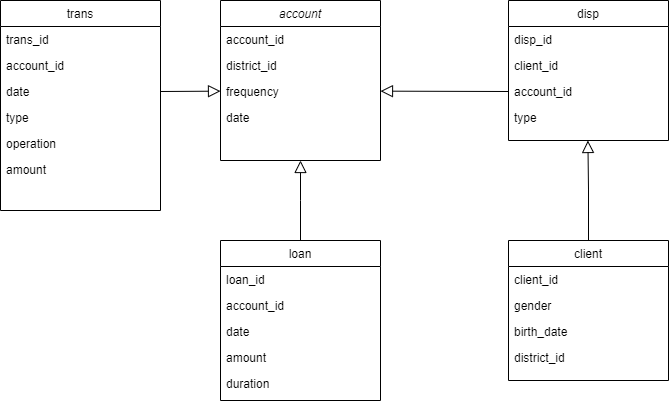
\includegraphics{./png/financial1.png}
\caption{Relacijski diagram}
\end{figure}

\hypertarget{kljuux10di}{%
\section{Ključi}\label{kljuux10di}}

Spremenljivkam, ki povezujejo razpredelnice, pravimo \textbf{ključi}. Te spremenljivke (ali zbirke spremenljivk) edinstveno definirajo podatke. Lahko gre za eno spremenljivko, kot je na primer \texttt{account\_id} v razpredelnici \texttt{account}. Lahko pa obstaja več spremenljivk, ki definirajo en podatek. Na primer, če imamo razpredelnico s temperaturami za vsak dan in uro. Potem ni nujno, da ima vsaka vrstica svoj ID, lahko pa jih edinstveno ločimo na podlagi dveh spremenljivk -- dneva in ure. V tem primeru gre torej za ključ, ki je sestavljen iz dveh spremenljivk.

Poznamo dva glavna tipa ključev:

\begin{itemize}
\tightlist
\item
  \textbf{Primarni ključ}. Ta ključ edinstveno definira podatek v razpredelnici. Na primer, \texttt{trans\_id} v razpredelnici \texttt{trans}. V urejenih podatkih ima vsaka tabela svoj primarni ključ.
\item
  \textbf{Tuj ključ}. To je ključ v razpredelnici, ki je primarni ključ v eni od preostalih razpredelnic. Na primer, \texttt{account\_id} v razpredelnici \texttt{trans}. Vrednosti tujih ključev se lahko podvajajo. Na primer, več transakcij lahko ima isto vrednost tujega ključa za \texttt{account\_id}, saj se na enem bančnem računu izvede več transakcij.
\end{itemize}

V kolikor razpredelnica nima primarnega ključa, lahko ustvarimo t. i. nadomestni ključ, ki igra vlogo primarnega ključa. To lahko naredimo na primer tako, da vsaki vrstici priredimo njeno zaporedno vrednost v razpredelnici. Na primer \texttt{mutate(row\_number())}.

Primarni in tuj ključ skupaj tvorita relacijo med razpredelnicama. Na primer \texttt{account\_id} predstavlja relacijo med razpredelnicama \texttt{trans} in \texttt{account}. Relacije so lahko ena-proti-ena (ena država ima enega predsednika in ena oseba je lahko predsednik samo ene države), ena-proti-mnogo (en igralec lahko igra za en klub, ampak en klub ima več igralcev) ali mnogo-proti-mnogo (en avtor lahko napiše več knjig in ena knjiga je lahko napisana s strani večih avtorjev).

Kadar imamo opravka z relacijskimi podatki, je smiselno preveriti, ali je primarni ključ res edinstven za vsako razpredelnico.

\begin{Shaded}
\begin{Highlighting}[]
\NormalTok{df\_list }\OtherTok{\textless{}{-}} \FunctionTok{list}\NormalTok{(account, client, disp, trans, loan)}
\NormalTok{id\_vec  }\OtherTok{\textless{}{-}} \FunctionTok{c}\NormalTok{(}\StringTok{"account\_id"}\NormalTok{, }\StringTok{"client\_id"}\NormalTok{, }\StringTok{"disp\_id"}\NormalTok{, }\StringTok{"trans\_id"}\NormalTok{, }\StringTok{"loan\_id"}\NormalTok{)}
\ControlFlowTok{for}\NormalTok{ (i }\ControlFlowTok{in} \DecValTok{1}\SpecialCharTok{:}\FunctionTok{length}\NormalTok{(df\_list)) \{}
\NormalTok{  tmp }\OtherTok{\textless{}{-}}\NormalTok{ df\_list[[i]] }\SpecialCharTok{\%\textgreater{}\%}
    \FunctionTok{group\_by}\NormalTok{(.data[[id\_vec[i]]]) }\SpecialCharTok{\%\textgreater{}\%}
    \FunctionTok{summarise}\NormalTok{(}\AttributeTok{n =} \FunctionTok{n}\NormalTok{()) }\SpecialCharTok{\%\textgreater{}\%}
    \FunctionTok{filter}\NormalTok{(n }\SpecialCharTok{\textgreater{}} \DecValTok{1}\NormalTok{)}
  \FunctionTok{print}\NormalTok{(tmp)}
\NormalTok{\}}
\end{Highlighting}
\end{Shaded}

\begin{verbatim}
## # A tibble: 0 x 2
## # ... with 2 variables: account_id <dbl>, n <int>
## # A tibble: 0 x 2
## # ... with 2 variables: client_id <dbl>, n <int>
## # A tibble: 0 x 2
## # ... with 2 variables: disp_id <dbl>, n <int>
## # A tibble: 0 x 2
## # ... with 2 variables: trans_id <dbl>, n <int>
## # A tibble: 0 x 2
## # ... with 2 variables: loan_id <dbl>, n <int>
\end{verbatim}

V prejšnjem klicu kode se pojavi nova sintaksa, in sicer \texttt{.data{[}{[}id\_vec{[}i{]}{]}{]}}. Funkcija \texttt{group\_by()} uporablja t. i. \emph{tidyselect}, s katerim izbiramo stolpce brez da bi jih dali v narekovaje. To pa predstavlja težavo, kadar so imena stolpcev shranjena v neki spremenljivki, kot v tem primeru. Tidyverse je ustvarjen na načelu, da olajša bolj pogoste operacije (na primer, enostavno uporaba \texttt{group\_by()} pri urejanju posamezne razpredelnice), za ceno težje izvedbe manj pogostih operacij (na primer, uporaba \texttt{group\_by()} v zanki for). Veliko večino urejanja podatkov bomo lahko z uporabo tidyverse naredili brez uporabe zank ali naprednih lastnih funkcij. V kolikor se boste lotili bolj programerskega pristopa, pa predlagamo, da si preberete navodila za programiranje z dplyr, ki jih dobite tako, da v konzoli kličete \texttt{vignette(\textquotesingle{}programming\textquotesingle{})}. Na tej delavnici ne bomo predstavili podrobnosti teh pristopov. Zaenkrat je dovolj, da poznamo samo zgornji klic. Torej, če imamo imena stolpcev shranjena v neki spremenljivki, potem moramo znotraj tidyselecta uporabiti \texttt{.data{[}{[}\textless{}spremenljivka-z-imeni-stolpcev\textgreater{}{]}{]}}.

\hypertarget{zdruux17eevanja}{%
\section{Združevanja}\label{zdruux17eevanja}}

Kadar imamo opravka z večimi razpredelnicami potrebujemo orodja, s katerimi lahko posamezne pare razpredelnic združimo. Vešči uporabniki R morda že poznajo funkcijo \texttt{merge}, ki je del osnovne različice R in je namenjena splošnemu združevanju razpredelnic. Seveda pa tidyverse premore svoje različice podobnih funkcij, ki premorejo enake lastnosti kot preostale funkcije v tej zbirki -- prejmejo in vrnejo podatke v enakem formatu in sicer tibblu. Poleg tega so funkcije iz paketa dplyr tudi hitrejše od \texttt{merge}, kar ima pomembno vlogo, kadar imamo opravka z nekoliko večjimi podatkovnimi množicami.

Združevanja podatkovnih razpredelnic lahko ločimo na 3 sklope:

\begin{itemize}
\tightlist
\item
  \textbf{Mutirajoča združevanja} (ang. \textbf{mutating joins}). Dodajo nove stolpce k razpredelnici iz ujemajočih vrstic druge razpredelnice.
\item
  \textbf{Filtrirajoča združevanja} (ang. \textbf{filtering joins}). Izberejo vrstice ene razpredenice glede na to, ali se te ujemajo z vrsticami v drugi razpredelnici.
\item
  \textbf{Operacije nad množicami}. Operirajo nad vrsticami, kot da so ti deli množice.
\end{itemize}

\hypertarget{mutirajoux10da-zdruux17eevanja}{%
\subsection{Mutirajoča združevanja}\label{mutirajoux10da-zdruux17eevanja}}

Mutirajoča združevanja so pogosta operacija pri delu z relacijskimi podatki. Te operacije združijo dve (ali več) razpredelnici glede na vrednosti stolpcev. Obstajajo 4 takšne operacije:

\begin{itemize}
\tightlist
\item
  \texttt{left\_join()}. Ohrani vse vrstice prve (leve) razpredelnice in poveže ustrezne vrstice iz druge razpredelnice s temi vrsticami.
\item
  \texttt{right\_join()}. Ohrani vse vrstice druge (desne) razpredelnice in poveže ustrezne vrstice iz prve rapredelnice s temi vrsticami.
\item
  \texttt{full\_join()}. Ohrani vse vrstice obeh razpredelnic.
\item
  \texttt{inner\_join()}. Ohrani samo tiste vrstice, ki se pojavijo v obeh razpredelnicah.
\end{itemize}

Prvi trije so tako imenovani zunanji stiki (\emph{outer join}), saj uporabijo vrstice, ki se pojavijo vsaj v eni razpredelnici. Za lažje razumevanje bomo najprej prikazali uporabo stikov na podatkih, ki jih bomo ustvarili sami. Sintaksa pri vseh združevanjih je:

\begin{Shaded}
\begin{Highlighting}[]
\FunctionTok{left\_join}\NormalTok{(}\SpecialCharTok{\textless{}}\NormalTok{razpredelnica1}\SpecialCharTok{\textgreater{}}\NormalTok{, }\SpecialCharTok{\textless{}}\NormalTok{razpredelnica2}\SpecialCharTok{\textgreater{}}\NormalTok{)}
\end{Highlighting}
\end{Shaded}

Ustvarimo dva tibbla:

\begin{Shaded}
\begin{Highlighting}[]
\NormalTok{df1 }\OtherTok{\textless{}{-}} \FunctionTok{tibble}\NormalTok{(}
  \AttributeTok{id =} \FunctionTok{c}\NormalTok{(}\StringTok{"id1"}\NormalTok{, }\StringTok{"id2"}\NormalTok{, }\StringTok{"id3"}\NormalTok{, }\StringTok{"id4"}\NormalTok{),}
  \AttributeTok{x =} \FunctionTok{c}\NormalTok{(}\DecValTok{4}\NormalTok{, }\DecValTok{6}\NormalTok{, }\DecValTok{1}\NormalTok{, }\DecValTok{2}\NormalTok{)}
\NormalTok{)}

\NormalTok{df2 }\OtherTok{\textless{}{-}} \FunctionTok{tibble}\NormalTok{(}
  \AttributeTok{id =} \FunctionTok{c}\NormalTok{(}\StringTok{"id1"}\NormalTok{, }\StringTok{"id3"}\NormalTok{, }\StringTok{"id4"}\NormalTok{, }\StringTok{"id5"}\NormalTok{),}
  \AttributeTok{y =} \FunctionTok{c}\NormalTok{(}\DecValTok{20}\NormalTok{, }\DecValTok{52}\NormalTok{, }\DecValTok{11}\NormalTok{, }\DecValTok{21}\NormalTok{)}
\NormalTok{)}
\NormalTok{df1}
\end{Highlighting}
\end{Shaded}

\begin{verbatim}
## # A tibble: 4 x 2
##   id        x
##   <chr> <dbl>
## 1 id1       4
## 2 id2       6
## 3 id3       1
## 4 id4       2
\end{verbatim}

\begin{Shaded}
\begin{Highlighting}[]
\NormalTok{df2}
\end{Highlighting}
\end{Shaded}

\begin{verbatim}
## # A tibble: 4 x 2
##   id        y
##   <chr> <dbl>
## 1 id1      20
## 2 id3      52
## 3 id4      11
## 4 id5      21
\end{verbatim}

\begin{itemize}
\tightlist
\item
  \texttt{left\_join()} obdrži tibble \texttt{df1} takšen kot je in mu pripne stolpec \texttt{y} iz tibbla \texttt{df2}, kjer so vrednosti spremenljivke \texttt{id} enake. Za tiste vrstice \texttt{df1}, ki nimajo ustreznega \texttt{id} v \texttt{df2} se vrednosti v spremenljivki \texttt{y} nastavijo na \texttt{NA}.
\end{itemize}

\begin{Shaded}
\begin{Highlighting}[]
\FunctionTok{left\_join}\NormalTok{(df1, df2)}
\end{Highlighting}
\end{Shaded}

\begin{verbatim}
## # A tibble: 4 x 3
##   id        x     y
##   <chr> <dbl> <dbl>
## 1 id1       4    20
## 2 id2       6    NA
## 3 id3       1    52
## 4 id4       2    11
\end{verbatim}

\begin{itemize}
\tightlist
\item
  \texttt{right\_join()} obdrži tibble \texttt{df2} takšen kot je in mu pripne stolpec \texttt{x} iz tibbla \texttt{df1}, kjer so vrednosti spremenljivke \texttt{id} enake. Za tiste vrstice \texttt{df2}, ki nimajo ustreznega \texttt{id} v \texttt{df1}, se vrednosti v spremenljivki \texttt{y} nastavijo na \texttt{NA}.
\end{itemize}

\begin{Shaded}
\begin{Highlighting}[]
\FunctionTok{right\_join}\NormalTok{(df1, df2)}
\end{Highlighting}
\end{Shaded}

\begin{verbatim}
## # A tibble: 4 x 3
##   id        x     y
##   <chr> <dbl> <dbl>
## 1 id1       4    20
## 2 id3       1    52
## 3 id4       2    11
## 4 id5      NA    21
\end{verbatim}

\begin{itemize}
\tightlist
\item
  \texttt{inner\_join()} obdrži samo tiste podatke, kjer se \texttt{id} nahaja v obeh razpredelnicah (torej 1, 3 in 4). Vse preostale vrstice zavrže.
\end{itemize}

\begin{Shaded}
\begin{Highlighting}[]
\FunctionTok{inner\_join}\NormalTok{(df1, df2)}
\end{Highlighting}
\end{Shaded}

\begin{verbatim}
## # A tibble: 3 x 3
##   id        x     y
##   <chr> <dbl> <dbl>
## 1 id1       4    20
## 2 id3       1    52
## 3 id4       2    11
\end{verbatim}

\begin{itemize}
\tightlist
\item
  \texttt{full\_join()} obdrži vse podatke iz \texttt{df1} in \texttt{df2}. Kjer ni ustreznega \texttt{id} v nasprotni razpredelnici se vrednosti nastavijo na \texttt{NA}.
\end{itemize}

\begin{Shaded}
\begin{Highlighting}[]
\FunctionTok{full\_join}\NormalTok{(df1, df2)}
\end{Highlighting}
\end{Shaded}

\begin{verbatim}
## # A tibble: 5 x 3
##   id        x     y
##   <chr> <dbl> <dbl>
## 1 id1       4    20
## 2 id2       6    NA
## 3 id3       1    52
## 4 id4       2    11
## 5 id5      NA    21
\end{verbatim}

Najbolj pogosto bomo uporabljali \texttt{left\_join()}, kadar bo cilj obdržati originalno razpredelnico, kot je, ali \texttt{inner\_join()}, kadar bomo želeli podatke brez manjkajočih vrednosti. Stik \texttt{right\_join()} je samo drugače usmerjen \texttt{left\_join()}.

Do sedaj smo prikazovali, kako združimo razpredelnice glede na primarni ključ, za katerega predpostavljamo, da je unikaten. Torej vsaka vrstica ima svoj ključ, ki se v razpredelnici ne ponovi. Včasih pa razpredelnice združujemo glede na sekundarni ključ. V tem primeru se lahko zgodi, da imamo relacijo ena-proti-mnogo. Če vzamemo bančne podatke od zgoraj ima lahko en račun več skrbnikov. Kaj se zgodi v tem primeru? Kaj pa če združimo transakcije in osebe glede na račun? En račun ima lahko več transakcij in več skrbnikov. Ker pri obeh razpredelnicah uporabimo sekundarni ključ, bomo najverjetneje dobili podvojene vrednosti pri obeh. Poglejmo si sedaj na primeru podatkov, ki jih generiramo sami.

\begin{Shaded}
\begin{Highlighting}[]
\NormalTok{df3 }\OtherTok{\textless{}{-}} \FunctionTok{tibble}\NormalTok{(}
  \AttributeTok{id1 =} \FunctionTok{c}\NormalTok{(}\StringTok{"id1"}\NormalTok{, }\StringTok{"id2"}\NormalTok{, }\StringTok{"id3"}\NormalTok{, }\StringTok{"id4"}\NormalTok{),}
  \AttributeTok{id2 =} \FunctionTok{c}\NormalTok{(}\StringTok{"id1"}\NormalTok{, }\StringTok{"id1"}\NormalTok{, }\StringTok{"id3"}\NormalTok{, }\StringTok{"id4"}\NormalTok{),}
  \AttributeTok{x =} \FunctionTok{c}\NormalTok{(}\DecValTok{5}\NormalTok{, }\DecValTok{6}\NormalTok{, }\DecValTok{1}\NormalTok{, }\DecValTok{2}\NormalTok{)}
\NormalTok{)}
\NormalTok{df4 }\OtherTok{\textless{}{-}} \FunctionTok{tibble}\NormalTok{(}
  \AttributeTok{id2 =} \FunctionTok{c}\NormalTok{(}\StringTok{"id1"}\NormalTok{, }\StringTok{"id2"}\NormalTok{, }\StringTok{"id3"}\NormalTok{),}
  \AttributeTok{y =} \FunctionTok{c}\NormalTok{(}\DecValTok{20}\NormalTok{, }\DecValTok{52}\NormalTok{, }\DecValTok{11}\NormalTok{)}
\NormalTok{)}
\NormalTok{df5 }\OtherTok{\textless{}{-}} \FunctionTok{tibble}\NormalTok{(}
  \AttributeTok{id3 =} \FunctionTok{c}\NormalTok{(}\StringTok{"id1"}\NormalTok{, }\StringTok{"id2"}\NormalTok{, }\StringTok{"id3"}\NormalTok{, }\StringTok{"id4"}\NormalTok{),}
  \AttributeTok{id2 =} \FunctionTok{c}\NormalTok{(}\StringTok{"id1"}\NormalTok{, }\StringTok{"id1"}\NormalTok{, }\StringTok{"id4"}\NormalTok{, }\StringTok{"id5"}\NormalTok{),}
  \AttributeTok{z =} \FunctionTok{c}\NormalTok{(}\DecValTok{5}\NormalTok{, }\DecValTok{1}\NormalTok{, }\DecValTok{23}\NormalTok{, }\DecValTok{5}\NormalTok{)}
\NormalTok{)}
\NormalTok{df3}
\end{Highlighting}
\end{Shaded}

\begin{verbatim}
## # A tibble: 4 x 3
##   id1   id2       x
##   <chr> <chr> <dbl>
## 1 id1   id1       5
## 2 id2   id1       6
## 3 id3   id3       1
## 4 id4   id4       2
\end{verbatim}

\begin{Shaded}
\begin{Highlighting}[]
\NormalTok{df4}
\end{Highlighting}
\end{Shaded}

\begin{verbatim}
## # A tibble: 3 x 2
##   id2       y
##   <chr> <dbl>
## 1 id1      20
## 2 id2      52
## 3 id3      11
\end{verbatim}

\begin{Shaded}
\begin{Highlighting}[]
\NormalTok{df5}
\end{Highlighting}
\end{Shaded}

\begin{verbatim}
## # A tibble: 4 x 3
##   id3   id2       z
##   <chr> <chr> <dbl>
## 1 id1   id1       5
## 2 id2   id1       1
## 3 id3   id4      23
## 4 id4   id5       5
\end{verbatim}

\texttt{df3} in \texttt{df5} imata podvojen sekundarni ključ. Združimo sedaj \texttt{df3} in \texttt{df4} z uporabo \texttt{inner\_join()}.

\begin{Shaded}
\begin{Highlighting}[]
\FunctionTok{inner\_join}\NormalTok{(df3, df4)}
\end{Highlighting}
\end{Shaded}

\begin{verbatim}
## # A tibble: 3 x 4
##   id1   id2       x     y
##   <chr> <chr> <dbl> <dbl>
## 1 id1   id1       5    20
## 2 id2   id1       6    20
## 3 id3   id3       1    11
\end{verbatim}

Ključ torej ostane podvojen. Kaj pa se zgodi, če imata obe razpredelnici podvojene ključe? V tem primeru dobimo kartezični produkt vseh podvojenih vrednosti:

\begin{Shaded}
\begin{Highlighting}[]
\FunctionTok{inner\_join}\NormalTok{(df3, df5)}
\end{Highlighting}
\end{Shaded}

\begin{verbatim}
## # A tibble: 5 x 5
##   id1   id2       x id3       z
##   <chr> <chr> <dbl> <chr> <dbl>
## 1 id1   id1       5 id1       5
## 2 id1   id1       5 id2       1
## 3 id2   id1       6 id1       5
## 4 id2   id1       6 id2       1
## 5 id4   id4       2 id3      23
\end{verbatim}

\texttt{df3} in \texttt{df5} imata podvojeno vrednost ključa \texttt{id1}. Torej dobimo vse kombinacije preostalih vrednosti (5, 5), (5, 1), (6, 5) in (6, 1).

\hypertarget{argument-by}{%
\subsection{\texorpdfstring{Argument \texttt{by}}{Argument by}}\label{argument-by}}

Združevanja, ki smo jih spoznali, privzeto združijo razpredelnici glede na vrednosti v vseh stolpcih, ki imajo enaka imena -- tamu pravimo tudi \textbf{naravno združevanje} (ang. \textbf{natural join}). Lahko pa tudi sami določimo, po katerih stolpcih želimo združiti podatke. To naredimo tako, da pri združevanjih uporabimo argument \texttt{by}. Sintaksa združevanj je potem:

\begin{Shaded}
\begin{Highlighting}[]
\FunctionTok{inner\_join}\NormalTok{(}\SpecialCharTok{\textless{}}\NormalTok{razpredelnica1}\SpecialCharTok{\textgreater{}}\NormalTok{, }\SpecialCharTok{\textless{}}\NormalTok{razpredelnica2}\SpecialCharTok{\textgreater{}}\NormalTok{, }\AttributeTok{by =} \SpecialCharTok{\textless{}}\NormalTok{vektor}\SpecialCharTok{{-}}\NormalTok{imen}\SpecialCharTok{{-}}\NormalTok{stolpcev}\SpecialCharTok{\textgreater{}}\NormalTok{)}
\end{Highlighting}
\end{Shaded}

\texttt{inner\_join()} dveh razpredelnic bi potem zapisali kot:

\begin{Shaded}
\begin{Highlighting}[]
\FunctionTok{inner\_join}\NormalTok{(df3, df4, }\AttributeTok{by =} \StringTok{"id2"}\NormalTok{)}
\end{Highlighting}
\end{Shaded}

\begin{verbatim}
## # A tibble: 3 x 4
##   id1   id2       x     y
##   <chr> <chr> <dbl> <dbl>
## 1 id1   id1       5    20
## 2 id2   id1       6    20
## 3 id3   id3       1    11
\end{verbatim}

Ta primer služi samo kot ilustracija in je uporaba \texttt{by} nepotrebna. Seveda pa se pri realnih podatkih velikokrat srečamo s stanjem, kjer ta argument potrebujemo. Prav tako je koda s parametrom \texttt{by} bolj robustna, saj sami definiramo, glede na katere stolpce naj se razpredelnice združujejo in ne more priti do kakšnih napak pri ponovljivosti.

Razpredelnici lahko združimo tudi po stolpcih, ki nimajo istega imena. Ni nenavadno, da imamo dve razpredelnici z enakimi spremenljivkami, ki pa so poimenovane drugače. Če bi želeli taki razpredelnici združiti glede na to spremenljivko, potem bi jo morali načeloma v eni razpredelnici preimenovati. S paketom dplyr pa lahko to naredimo tudi drugače. Združimo sedaj \texttt{df3} in \texttt{df5} glede na stolpca \texttt{x} in \texttt{z} ter skupni stolpec \texttt{id2}.

\begin{Shaded}
\begin{Highlighting}[]
\FunctionTok{inner\_join}\NormalTok{(df3, df5, }\AttributeTok{by =} \FunctionTok{c}\NormalTok{(}\StringTok{"x"} \OtherTok{=} \StringTok{"z"}\NormalTok{, }\StringTok{"id2"}\NormalTok{))}
\end{Highlighting}
\end{Shaded}

\begin{verbatim}
## # A tibble: 1 x 4
##   id1   id2       x id3  
##   <chr> <chr> <dbl> <chr>
## 1 id1   id1       5 id1
\end{verbatim}

\hypertarget{filtrirajoux10da-zdruux17eevanja}{%
\subsection{Filtrirajoča združevanja}\label{filtrirajoux10da-zdruux17eevanja}}

Pri filtrirajočih združevanjih ne gre toliko za združevanja, kolikor gre za izbiro posameznih vrstic, glede na ujemanje vrednotsti stolpcev v neki drugi razpredelnici. Poznamo 2 takšni združevanji:

\begin{itemize}
\tightlist
\item
  \texttt{semi\_join()}. Obdrži vse vrstice v prvi razpredelnici, ki ustrezajo vrsticam v drugi razpredelnici.
\item
  \texttt{anti\_join()}. Izloči vse vrstice v prvi razpredelnici, ki ustrezajo vrsticam v drugi razpredelnici.
\end{itemize}

Poglejmo si uporabo teh združevanj na naših generiranih razpredelnicah.

\begin{Shaded}
\begin{Highlighting}[]
\NormalTok{df1}
\end{Highlighting}
\end{Shaded}

\begin{verbatim}
## # A tibble: 4 x 2
##   id        x
##   <chr> <dbl>
## 1 id1       4
## 2 id2       6
## 3 id3       1
## 4 id4       2
\end{verbatim}

\begin{Shaded}
\begin{Highlighting}[]
\NormalTok{df2}
\end{Highlighting}
\end{Shaded}

\begin{verbatim}
## # A tibble: 4 x 2
##   id        y
##   <chr> <dbl>
## 1 id1      20
## 2 id3      52
## 3 id4      11
## 4 id5      21
\end{verbatim}

\begin{Shaded}
\begin{Highlighting}[]
\FunctionTok{semi\_join}\NormalTok{(df1, df2)}
\end{Highlighting}
\end{Shaded}

\begin{verbatim}
## # A tibble: 3 x 2
##   id        x
##   <chr> <dbl>
## 1 id1       4
## 2 id3       1
## 3 id4       2
\end{verbatim}

\texttt{semi\_join()} je torej izločil vrstico z \texttt{id2}, saj se ta ne pojavi v \texttt{df2}.

\begin{Shaded}
\begin{Highlighting}[]
\FunctionTok{anti\_join}\NormalTok{(df1, df2)}
\end{Highlighting}
\end{Shaded}

\begin{verbatim}
## # A tibble: 1 x 2
##   id        x
##   <chr> <dbl>
## 1 id2       6
\end{verbatim}

\texttt{semi\_join()} je torej izločil vse vrstice, ki se pojavijo tudi v \texttt{df2}. Ostane torej samo vrstica z \texttt{id2}.

\hypertarget{zdruux17eevanja-na-realnih-podatkih}{%
\subsection{Združevanja na realnih podatkih}\label{zdruux17eevanja-na-realnih-podatkih}}

Sedaj, ko smo spoznali glavne lastnosti različnih združevanj na primerih, ki so nam omogočali lažjo predstavo, pa se posvetimo realnim podatkom, ki smo jih predstavili v začetku tega poglavja. Imamo torej podatke o bančnih računih, transakcijah, posojilih, skrbnikih računov in povezovalno razpredelnico med računi in skrbniki. Lotimo se sedaj relativno enostavne analize, kjer bomo naredili sledeče:

\begin{enumerate}
\def\labelenumi{\arabic{enumi})}
\tightlist
\item
  Ustvarili novo razpredelnico, kjer bomo imeli podatke o vseh bančnih računih in o lastnikih teh računov. Lastnik računa je lahko samo en, medtem ko je skrbnikov lahko več.
\item
  Filtrirali razpredelnico iz točke 1), v kateri bodo samo tisti, ki imajo posojila nad 100000 kron.
\item
  Ustvarili novo razpredelnico klientov, kjer bomo imeli podatke o klientih in posojilih in bodo zajeti samo klienti s posojili.
\item
  Izračunali kateri klienti, ki imajo posojilo, imajo tudi največ transakcij.
\end{enumerate}

Za vsakega izmed teh korakov bomo morali uporabiti eno od združevanj, ki smo jih spoznali. Na primer, v samih razpredelnicah nimamo direktne povezave med komitenti in transakcijami, tako da bomo morali zadeve nekako združiti. Podobno velja za ostale alineje.

Najprej želimo združiti razpredelnici \texttt{account} in \texttt{client}. Za to bomo potrebovali povezovalno razpredelnico \texttt{disp} v kateri se tudi nahaja informacija o tem, ali je klient lastnik ali samo skrbnik računa. Najprej povežemo razpredelnico \texttt{account} z razpredelnico \texttt{disp} in filtriramo glede na tip klienta:

\begin{Shaded}
\begin{Highlighting}[]
\NormalTok{account\_disp }\OtherTok{\textless{}{-}} \FunctionTok{left\_join}\NormalTok{(account, disp) }\SpecialCharTok{\%\textgreater{}\%}
  \FunctionTok{filter}\NormalTok{(type }\SpecialCharTok{==} \StringTok{"OWNER"}\NormalTok{)}
\NormalTok{account\_disp}
\end{Highlighting}
\end{Shaded}

\begin{verbatim}
## # A tibble: 4,500 x 7
##    account_id district_id frequency       date       disp_id client_id type 
##         <dbl>       <dbl> <chr>           <date>       <dbl>     <dbl> <chr>
##  1          1          18 monthly payment 1995-03-24       1         1 OWNER
##  2          2           1 monthly payment 1993-02-26       2         2 OWNER
##  3          3           5 monthly payment 1997-07-07       4         4 OWNER
##  4          4          12 monthly payment 1996-02-21       6         6 OWNER
##  5          5          15 monthly payment 1997-05-30       7         7 OWNER
##  6          6          51 monthly payment 1994-09-27       8         8 OWNER
##  7          7          60 monthly payment 1996-11-24       9         9 OWNER
##  8          8          57 monthly payment 1995-09-21      10        10 OWNER
##  9          9          70 monthly payment 1993-01-27      12        12 OWNER
## 10         10          54 monthly payment 1996-08-28      13        13 OWNER
## # ... with 4,490 more rows
\end{verbatim}

Sedaj lahko to novo razpredelnico povežemo z razpredelnico \texttt{client}.

\begin{Shaded}
\begin{Highlighting}[]
\NormalTok{account\_client }\OtherTok{\textless{}{-}} \FunctionTok{left\_join}\NormalTok{(account\_disp, client)}
\end{Highlighting}
\end{Shaded}

S tem smo dobili željeno razpredelnico, v kateri imamo za vsak račun tudi informacijo o lastniku. Kot drugi korak želimo ustvariti razpredelnico, v kateri bodo samo podatki o klientih, ki imajo posojila v vrednosti več kot 100000 kron. Najprej ustvarimo razpredelnico, v kateri so samo takšna posojila, nato pa uporabimo \texttt{semi\_join()}, ki bo iz razpredelnice \texttt{account\_client} izbral samo vrstice, ki se bodo ujemale z vrsticami v tej novi razpredelnici posojil.

\begin{Shaded}
\begin{Highlighting}[]
\NormalTok{loan\_100k }\OtherTok{\textless{}{-}}\NormalTok{ loan }\SpecialCharTok{\%\textgreater{}\%}
  \FunctionTok{filter}\NormalTok{(amount }\SpecialCharTok{\textgreater{}} \DecValTok{100000}\NormalTok{)}
\NormalTok{account\_100k }\OtherTok{\textless{}{-}} \FunctionTok{semi\_join}\NormalTok{(account\_client, loan\_100k)}
\NormalTok{account\_100k}
\end{Highlighting}
\end{Shaded}

\begin{verbatim}
## # A tibble: 0 x 9
## # ... with 9 variables: account_id <dbl>, district_id <dbl>, frequency <chr>,
## #   date <date>, disp_id <dbl>, client_id <dbl>, type <chr>, gender <chr>,
## #   birth_date <date>
\end{verbatim}

Hm\ldots dobili smo prazen tibble, čeprav obstajajo tako velika posojila. Zakaj je do tega prišlo? V obeh razpredelnicah se nahajata spremenjivki \texttt{account\_id} in \texttt{date}. Ampak spremenljivka \texttt{date} ni ista spremenljivka, pri razpredelnici \texttt{account\_client} predstavlja, kdaj je bil račun odprt, pri \texttt{loan\_100k} pa predstavlja kdaj je bilo posojilo odobreno. Torej po tej spremenljivki ne smemo združevati. Uporabimo \texttt{by}:

\begin{Shaded}
\begin{Highlighting}[]
\NormalTok{account\_100k }\OtherTok{\textless{}{-}} \FunctionTok{semi\_join}\NormalTok{(account\_client, loan\_100k, }\AttributeTok{by =} \StringTok{"account\_id"}\NormalTok{)}
\NormalTok{account\_100k}
\end{Highlighting}
\end{Shaded}

\begin{verbatim}
## # A tibble: 377 x 9
##    account_id district_id frequency    date       disp_id client_id type  gender
##         <dbl>       <dbl> <chr>        <date>       <dbl>     <dbl> <chr> <chr> 
##  1         37          20 monthly pay~ 1997-08-18      45        45 OWNER M     
##  2         38          19 weekly paym~ 1997-08-08      46        46 OWNER F     
##  3         67          16 monthly pay~ 1994-10-19      78        78 OWNER F     
##  4         97          74 monthly pay~ 1996-05-05     116       116 OWNER M     
##  5        103          44 monthly pay~ 1996-03-10     124       124 OWNER M     
##  6        105          21 monthly pay~ 1997-07-10     127       127 OWNER F     
##  7        110          36 monthly pay~ 1996-07-17     132       132 OWNER M     
##  8        173          66 monthly pay~ 1993-11-26     210       210 OWNER M     
##  9        226          70 monthly pay~ 1997-02-23     272       272 OWNER F     
## 10        276          38 monthly pay~ 1997-12-08     333       333 OWNER M     
## # ... with 367 more rows, and 1 more variable: birth_date <date>
\end{verbatim}

V naslednjem koraku želimo imeti podatke o klientih in posojilih. Najprej bomo morali združiti razpredelnici \texttt{client} in \texttt{disp}, nato pa dodati še razpredelnico \texttt{loan}. Ustvarimo to novo razpredelnico kar z uporabo operatorja \texttt{\%\textgreater{}\%}:

\begin{Shaded}
\begin{Highlighting}[]
\NormalTok{client\_loan }\OtherTok{\textless{}{-}}\NormalTok{ client }\SpecialCharTok{\%\textgreater{}\%}
  \FunctionTok{left\_join}\NormalTok{(disp) }\SpecialCharTok{\%\textgreater{}\%}
  \FunctionTok{inner\_join}\NormalTok{(loan, }\AttributeTok{by =} \StringTok{"account\_id"}\NormalTok{)}
\NormalTok{client\_loan}
\end{Highlighting}
\end{Shaded}

\begin{verbatim}
## # A tibble: 827 x 13
##    client_id gender birth_date district_id disp_id account_id type      loan_id
##        <dbl> <chr>  <date>           <dbl>   <dbl>      <dbl> <chr>       <dbl>
##  1         2 M      1945-02-04           1       2          2 OWNER        4959
##  2         3 F      1940-10-09           1       3          2 DISPONENT    4959
##  3        25 F      1939-04-23          21      25         19 OWNER        4961
##  4        31 M      1962-02-09          68      31         25 OWNER        4962
##  5        45 M      1952-08-26          20      45         37 OWNER        4967
##  6        46 F      1940-01-30          19      46         38 OWNER        4968
##  7        78 F      1944-06-13          16      78         67 OWNER        4973
##  8       116 M      1942-01-28          74     116         97 OWNER        4986
##  9       117 F      1936-09-20          74     117         97 DISPONENT    4986
## 10       124 M      1967-09-21          44     124        103 OWNER        4988
## # ... with 817 more rows, and 5 more variables: date <date>, amount <dbl>,
## #   duration <dbl>, payments <dbl>, status <chr>
\end{verbatim}

Na koncu preverimo še, kateri klienti, ki imajo posojilo, imajo največ transakcij. Za to bomo morali najprej izračunati število transakcij na vsakem bančnem računu. Uporabimo znanje, ki smo ga pridobili na prvem predavanju:

\begin{Shaded}
\begin{Highlighting}[]
\NormalTok{trans\_count }\OtherTok{\textless{}{-}}\NormalTok{ trans }\SpecialCharTok{\%\textgreater{}\%}
  \FunctionTok{group\_by}\NormalTok{(account\_id) }\SpecialCharTok{\%\textgreater{}\%}
  \FunctionTok{summarise}\NormalTok{(}\AttributeTok{n\_trans =} \FunctionTok{n}\NormalTok{())}
\NormalTok{trans\_count}
\end{Highlighting}
\end{Shaded}

\begin{verbatim}
## # A tibble: 4,205 x 2
##    account_id n_trans
##         <dbl>   <int>
##  1          1       6
##  2          2      10
##  3          3       3
##  4          4       6
##  5          5       3
##  6          6       8
##  7          7       3
##  8          8       7
##  9          9       3
## 10         10       1
## # ... with 4,195 more rows
\end{verbatim}

\begin{Shaded}
\begin{Highlighting}[]
\FunctionTok{left\_join}\NormalTok{(client\_loan, trans\_count) }\SpecialCharTok{\%\textgreater{}\%}
  \FunctionTok{arrange}\NormalTok{(}\FunctionTok{desc}\NormalTok{(n\_trans))}
\end{Highlighting}
\end{Shaded}

\begin{verbatim}
## # A tibble: 827 x 14
##    client_id gender birth_date district_id disp_id account_id type      loan_id
##        <dbl> <chr>  <date>           <dbl>   <dbl>      <dbl> <chr>       <dbl>
##  1     11126 F      1965-01-22           1   10818       9034 OWNER        6820
##  2      6367 M      1970-04-28          44    6367       5270 OWNER        6077
##  3      7291 F      1940-12-02          77    7291       6034 OWNER        6228
##  4      7195 M      1962-09-11          50    7195       5952 OWNER        6216
##  5      4620 F      1940-11-01          54    4620       3834 OWNER        5754
##  6      4621 M      1946-02-10          54    4621       3834 DISPONENT    5754
##  7     11461 M      1974-07-08          70   11153       9307 OWNER        6895
##  8     11866 M      1937-09-02           1   11558       9640 OWNER        6960
##  9     11867 F      1934-11-19           1   11559       9640 DISPONENT    6960
## 10     13657 F      1963-05-12          59   13349      11111 OWNER        7259
## # ... with 817 more rows, and 6 more variables: date <date>, amount <dbl>,
## #   duration <dbl>, payments <dbl>, status <chr>, n_trans <int>
\end{verbatim}

\hypertarget{operacije-nad-mnoux17eicami}{%
\section{Operacije nad množicami}\label{operacije-nad-mnoux17eicami}}

V tem poglavju si bomo ogledali operacije nad množicami. Te delujejo nad vektorji, prav tako pa nad \texttt{data.frame} oziroma nad tibbli. Poznamo 3 glavne operacije:

\begin{itemize}
\tightlist
\item
  \textbf{Unija}. Vrne vse elemente, ki se pojavijo v eni ali drugi množici.
\item
  \textbf{Presek}. Vrne vse elemente, ki se pojavijo v obeh množicah.
\item
  \textbf{Razlika}. Vrne vse elemente prve množice, ki se ne pojavijo v drugi množici.
\end{itemize}

Poglejmo si uporabo teh operacij nad tibbli.

\begin{Shaded}
\begin{Highlighting}[]
\NormalTok{df1 }\OtherTok{\textless{}{-}} \FunctionTok{tibble}\NormalTok{(}
  \AttributeTok{id =} \FunctionTok{c}\NormalTok{(}\StringTok{"id1"}\NormalTok{, }\StringTok{"id2"}\NormalTok{),}
  \AttributeTok{x =} \FunctionTok{c}\NormalTok{(}\DecValTok{4}\NormalTok{, }\DecValTok{6}\NormalTok{)}
\NormalTok{)}

\NormalTok{df2 }\OtherTok{\textless{}{-}} \FunctionTok{tibble}\NormalTok{(}
  \AttributeTok{id =} \FunctionTok{c}\NormalTok{(}\StringTok{"id1"}\NormalTok{, }\StringTok{"id3"}\NormalTok{),}
  \AttributeTok{x =} \FunctionTok{c}\NormalTok{(}\DecValTok{4}\NormalTok{, }\DecValTok{52}\NormalTok{)}
\NormalTok{)}
\NormalTok{df1}
\end{Highlighting}
\end{Shaded}

\begin{verbatim}
## # A tibble: 2 x 2
##   id        x
##   <chr> <dbl>
## 1 id1       4
## 2 id2       6
\end{verbatim}

\begin{Shaded}
\begin{Highlighting}[]
\NormalTok{df2}
\end{Highlighting}
\end{Shaded}

\begin{verbatim}
## # A tibble: 2 x 2
##   id        x
##   <chr> <dbl>
## 1 id1       4
## 2 id3      52
\end{verbatim}

\begin{Shaded}
\begin{Highlighting}[]
\FunctionTok{union}\NormalTok{(df1, df2)}
\end{Highlighting}
\end{Shaded}

\begin{verbatim}
## # A tibble: 3 x 2
##   id        x
##   <chr> <dbl>
## 1 id1       4
## 2 id2       6
## 3 id3      52
\end{verbatim}

\begin{Shaded}
\begin{Highlighting}[]
\FunctionTok{intersect}\NormalTok{(df1, df2)}
\end{Highlighting}
\end{Shaded}

\begin{verbatim}
## # A tibble: 1 x 2
##   id        x
##   <chr> <dbl>
## 1 id1       4
\end{verbatim}

\begin{Shaded}
\begin{Highlighting}[]
\FunctionTok{setdiff}\NormalTok{(df1, df2)}
\end{Highlighting}
\end{Shaded}

\begin{verbatim}
## # A tibble: 1 x 2
##   id        x
##   <chr> <dbl>
## 1 id2       6
\end{verbatim}

\begin{Shaded}
\begin{Highlighting}[]
\FunctionTok{setdiff}\NormalTok{(df2, df1)}
\end{Highlighting}
\end{Shaded}

\begin{verbatim}
## # A tibble: 1 x 2
##   id        x
##   <chr> <dbl>
## 1 id3      52
\end{verbatim}

\hypertarget{ali-ux17eelite-izvedeti-veux10d-1}{%
\section{Ali želite izvedeti več?}\label{ali-ux17eelite-izvedeti-veux10d-1}}

Hadley Wickham je objavil znanstveni članek na temo urejenih podatkov: \url{https://vita.had.co.nz/papers/tidy-data.pdf}, ki je vsekakor vreden branja. Za več informacij o neurejenih podatkih in v katerih primerih so lahko celo bolj zaželjeni, predlagamo ta blog: \url{https://simplystatistics.org/2016/02/17/non-tidy-data/}.

\hypertarget{domaux10da-naloga-1}{%
\section{Domača naloga}\label{domaux10da-naloga-1}}

\begin{enumerate}
\def\labelenumi{\arabic{enumi})}
\item
  Spodaj imamo podatke o stroških za 4 osebe. Razpredelnica je v neurejeni obliki. Vaša naloga je, da jo pretvorite v urejeno obliko.

\begin{Shaded}
\begin{Highlighting}[]
\NormalTok{podatki\_o\_stroskih }\OtherTok{\textless{}{-}} \FunctionTok{tibble}\NormalTok{(}
  \AttributeTok{ime =} \FunctionTok{c}\NormalTok{(}\StringTok{"Miha"}\NormalTok{, }\StringTok{"Ana"}\NormalTok{, }\StringTok{"Andrej"}\NormalTok{, }\StringTok{"Maja"}\NormalTok{),}
  \AttributeTok{april\_2019 =} \FunctionTok{c}\NormalTok{(}\DecValTok{400}\NormalTok{, }\DecValTok{200}\NormalTok{, }\DecValTok{300}\NormalTok{, }\DecValTok{350}\NormalTok{),}
  \AttributeTok{maj\_2019 =} \FunctionTok{c}\NormalTok{(}\DecValTok{390}\NormalTok{, }\DecValTok{250}\NormalTok{, }\DecValTok{280}\NormalTok{, }\DecValTok{400}\NormalTok{),}
  \AttributeTok{april\_2020 =} \FunctionTok{c}\NormalTok{(}\DecValTok{410}\NormalTok{, }\DecValTok{150}\NormalTok{, }\DecValTok{500}\NormalTok{, }\DecValTok{400}\NormalTok{),}
  \AttributeTok{maj\_2020 =} \FunctionTok{c}\NormalTok{(}\DecValTok{300}\NormalTok{, }\DecValTok{320}\NormalTok{, }\DecValTok{550}\NormalTok{, }\DecValTok{320}\NormalTok{)}
\NormalTok{)}
\end{Highlighting}
\end{Shaded}

  Rešitev:

\begin{verbatim}
## # A tibble: 16 x 4
##    ime    mesec leto  strosek
##    <chr>  <chr> <chr>   <dbl>
##  1 Miha   april 2019      400
##  2 Miha   maj   2019      390
##  3 Miha   april 2020      410
##  4 Miha   maj   2020      300
##  5 Ana    april 2019      200
##  6 Ana    maj   2019      250
##  7 Ana    april 2020      150
##  8 Ana    maj   2020      320
##  9 Andrej april 2019      300
## 10 Andrej maj   2019      280
## 11 Andrej april 2020      500
## 12 Andrej maj   2020      550
## 13 Maja   april 2019      350
## 14 Maja   maj   2019      400
## 15 Maja   april 2020      400
## 16 Maja   maj   2020      320
\end{verbatim}
\item
  V mapi \emph{data-raw} se nahajajo podatki o predsedniških volitvah v ZDA. Najprej izberite samo podmnožico vrstic, kjer sta kandidata Joe Biden ali Donald Trump, in izločite stolpec \texttt{party}. Nato pretvorite podatke v širšo obliko, tako da bo vsak izmed kandidatov imel svoj stolpec.

\begin{verbatim}
## # A tibble: 4,633 x 4
##    state                county               `Joe Biden` `Donald Trump`
##    <chr>                <chr>                      <dbl>          <dbl>
##  1 Delaware             Kent County                44518          40976
##  2 Delaware             New Castle County         194238          87685
##  3 Delaware             Sussex County              56657          71196
##  4 District of Columbia District of Columbia       29509           1149
##  5 District of Columbia Ward 2                     24247           2365
##  6 District of Columbia Ward 3                     33584           2972
##  7 District of Columbia Ward 4                     35117           1467
##  8 District of Columbia Ward 5                     36585           1416
##  9 District of Columbia Ward 6                     44699           3360
## 10 District of Columbia Ward 7                     30253            885
## # ... with 4,623 more rows
\end{verbatim}
\item
  Pri bančnih podatkih smo zaenkrat delali samo s petimi razpredelnicami. Celotna zbirka je nekoliko večja, saj vsebuje še 3 razpredelnice. V mapi \emph{data-raw/financial-hw/} se nahajajo še preostale razpredelnice. Pri nalogi bomo uporabili razpredelnico \emph{district}, ki vsebuje podatke o okrajih. Vsekakor pa se lahko za lastno vajo poigrate še s preostalima dvema. Vaše naloge so:
\end{enumerate}

\begin{itemize}
\item
  Preberite podatke o okrajih v R.
\item
  Ugotovite, kaj je primarni ključ te razpredelnice.
\item
  Ustrezno dopolnite entitetni diagram. To lahko naredite ročno, v kolikor pa se želite naučiti narediti bolj profesionalne diagrame pa predlagamo spletno orodje \url{https://app.diagrams.net/}. V mapi \emph{support-files} se nahaja naš diagram. Tega lahko enostavno naložite v to orodje in ga dopolnite.
\item
  Poiščite 3 pokrajine (A3) z največjo povprečno vrednostjo posojil.

\begin{verbatim}
## # A tibble: 3 x 2
##   A3              mean_loan
##   <chr>               <dbl>
## 1 east Bohemia      165997.
## 2 south Bohemia     156236.
## 3 central Bohemia   155392.
\end{verbatim}
\end{itemize}

\begin{enumerate}
\def\labelenumi{\arabic{enumi})}
\setcounter{enumi}{3}
\tightlist
\item
  \textbf{Težka naloga}. Namestite paket \emph{nycflights13}. Gre za relacijsko podatkovno zbirko o letih iz New Yorka v letu 2013. Naložite podatke z \texttt{library(nycflights13)}. Uporabljali bomo štiri razpredelnice: flights, weather, airlines in planes. Vaša naloga je:
\end{enumerate}

\begin{itemize}
\item
  Poizkusite najti primarni ključ za razpredelnico \texttt{flights}. Ali gre za primarni ključ lahko preverite tako, da preverite ali ta ključ unikatno določa vrstico v podatkih, torej da preštejete podatke, grupirane glede na ta ključ. Ključ je lahko sestavljen tudi iz večih spremenljivk. Na prvi pogled bi rekli, da je primarni ključ številka leta, ampak temu ni tako (preverimo s štetjem). Ali je morda kakšna druga kombinacija spremenljivk? Lahko da razpredelnica nima primarnega ključa. V tem primeru določite nadomestni ključ tako, da dodate stolpec ID z \texttt{mutate(ID\ =\ row\_number())}.
\item
  Ugotovite, kaj so primarni in kaj tuji ključi preostalih razpredelnic. Pri nekaterih razpredelnicah v tej zbirki bomo imeli sestavljene ključe, torej bodo ključi sestavljeni iz večih stolpcev. Namig: Pri vremenu je manjša napaka v podatkih in se tudi primarni ključ ponovi v zanemarljivem številu primerov. Vsekakor so napake v realnih podatkih pričakovane in moramo na to biti pozorni!
\item
  Narišite relacijski diagram.
\item
  Ustvarite novo razpredelnico tako da razpredelnici \texttt{flights} dodate podrobnosti o lastnostih letal za vsak let.

\begin{verbatim}
## # A tibble: 336,776 x 28
##       ID year.x month   day dep_time sched_dep_time dep_delay arr_time
##    <int>  <int> <int> <int>    <int>          <int>     <dbl>    <int>
##  1     1   2013     1     1      517            515         2      830
##  2     2   2013     1     1      533            529         4      850
##  3     3   2013     1     1      542            540         2      923
##  4     4   2013     1     1      544            545        -1     1004
##  5     5   2013     1     1      554            600        -6      812
##  6     6   2013     1     1      554            558        -4      740
##  7     7   2013     1     1      555            600        -5      913
##  8     8   2013     1     1      557            600        -3      709
##  9     9   2013     1     1      557            600        -3      838
## 10    10   2013     1     1      558            600        -2      753
## # ... with 336,766 more rows, and 20 more variables: sched_arr_time <int>,
## #   arr_delay <dbl>, carrier <chr>, flight <int>, tailnum <chr>, origin <chr>,
## #   dest <chr>, air_time <dbl>, distance <dbl>, hour <dbl>, minute <dbl>,
## #   time_hour <dttm>, year.y <int>, type <chr>, manufacturer <chr>,
## #   model <chr>, engines <int>, seats <int>, speed <int>, engine <chr>
\end{verbatim}
\item
  Ustvarite novo razpredelnico tako da razpredelnici \texttt{flights} dodate podrobnosti o vremenu na letališču vsak let.

\begin{verbatim}
## # A tibble: 336,776 x 30
##       ID  year month   day dep_time sched_dep_time dep_delay arr_time
##    <int> <int> <int> <int>    <int>          <int>     <dbl>    <int>
##  1     1  2013     1     1      517            515         2      830
##  2     2  2013     1     1      533            529         4      850
##  3     3  2013     1     1      542            540         2      923
##  4     4  2013     1     1      544            545        -1     1004
##  5     5  2013     1     1      554            600        -6      812
##  6     6  2013     1     1      554            558        -4      740
##  7     7  2013     1     1      555            600        -5      913
##  8     8  2013     1     1      557            600        -3      709
##  9     9  2013     1     1      557            600        -3      838
## 10    10  2013     1     1      558            600        -2      753
## # ... with 336,766 more rows, and 22 more variables: sched_arr_time <int>,
## #   arr_delay <dbl>, carrier <chr>, flight <int>, tailnum <chr>, origin <chr>,
## #   dest <chr>, air_time <dbl>, distance <dbl>, hour <dbl>, minute <dbl>,
## #   time_hour.x <dttm>, temp <dbl>, dewp <dbl>, humid <dbl>, wind_dir <dbl>,
## #   wind_speed <dbl>, wind_gust <dbl>, precip <dbl>, pressure <dbl>,
## #   visib <dbl>, time_hour.y <dttm>
\end{verbatim}
\item
  Poiščite vsa letala, ki so v New York priletela 5. aprila iz letališča Chicago Ohare Intl.

\begin{verbatim}
## # A tibble: 35 x 35
##        ID year.x month   day dep_time sched_dep_time dep_delay arr_time
##     <int>  <int> <int> <int>    <int>          <int>     <dbl>    <int>
##  1 169022   2013     4     5      545            600       -15      710
##  2 169051   2013     4     5      604            610        -6      739
##  3 169062   2013     4     5      624            630        -6      755
##  4 169086   2013     4     5      636            630         6      814
##  5 169100   2013     4     5      653            700        -7      827
##  6 169114   2013     4     5      659            700        -1      823
##  7 169125   2013     4     5      720            725        -5      851
##  8 169159   2013     4     5      752            759        -7      920
##  9 169183   2013     4     5      810            815        -5      933
## 10 169201   2013     4     5      823            830        -7      957
## # ... with 25 more rows, and 27 more variables: sched_arr_time <int>,
## #   arr_delay <dbl>, carrier <chr>, flight <int>, tailnum <chr>, origin <chr>,
## #   dest <chr>, air_time <dbl>, distance <dbl>, hour <dbl>, minute <dbl>,
## #   time_hour <dttm>, year.y <int>, type <chr>, manufacturer <chr>,
## #   model <chr>, engines <int>, seats <int>, speed <int>, engine <chr>,
## #   name <chr>, lat <dbl>, lon <dbl>, alt <dbl>, tz <dbl>, dst <chr>,
## #   tzone <chr>
\end{verbatim}
\end{itemize}

\begin{enumerate}
\def\labelenumi{\arabic{enumi})}
\setcounter{enumi}{4}
\item
  \textbf{Zelo težka naloga}. V mapi \emph{data-raw} se nahajajo podatki o kreditnih karticah v Tajvanu \emph{default of credit card clients.xlsx}. Pridobili smo jih iz UCI Machine Learning repozitorija \citep{Dua2019}. Podatki so bili uporabljeni v znanstveni raziskavi \citep{Yeh2009}, kjer so napovedovali verjetnosti neplačil v odvisnosti od preteklih transakcij na kartici in podatkov o lastnikih. Podatki so v xlsx datoteki. Bodite pozorni, da je prva vrstica datoteke nepomembna in se glava začne komaj v drugi vrstici. Trenutno so podatki v obliki, v kateri so zelo primerni kot vhodni podatek za kak model, na primer linearno regresijo. Vsekakor pa niso v primerni obliki za učinkotivo urejanje in hranjenje. Vaša naloga je, da podatke preberete v R in razpredelnico pretvorite v urejeno obliko.

  Predlagamo, da nalogo poizkusite rešiti sami. Naloga zahteva precej razmisleka in tudi nekaj samostojne raziskave (na primer, kaj posamezni stolpci pomenijo -- pomagate si lahko s spletno stranjo, iz katere smo prenesli podatke). V kolikor se vam zatakne, smo vam spodaj pripravili nekaj namigov:
\end{enumerate}

\begin{itemize}
\item
  Najprej je potrebno razmisliti, kaj so spremenljivke. Na primer, ali sta \texttt{PAY\_1} in \texttt{PAY\_2} 2 spremenljivki, ali predstavljata 1 spremenljivko, ki pa je razdeljena glede na neko drugo spremenljivko?
\item
  Predlagamo da začnete ukaze tako, da razpredelnico spremenite v daljšo obliko, kjer vse spremenljivke, ki se pojavijo v večih stolpcih, shranite v 1 stolpec.
\item
  V novem stolpcu so celice sestavljene iz 2 spremenljivk. Ena od teh je ID meseca. Torej moramo ta stolpec ločiti na 2 stolpca. Katero funkcijo uporabimo za to? Pri tem bo prav prišel tudi argument te funkcije \texttt{sep\ =\ -1}, ki bo stolpec ločil na zadnji znak v besedi in vse preostalo (na primer, ``beseda3'' bo razdelil na ``beseda'' in ``3''). -1 predstavlja pri koliko znakih od konca proti začetku naredimo ločitev besede.
\item
  V enem od teh dveh preostalih stolpcev imamo še vedno shranjene 3 spremenljivke, za katere bi bilo bolje, če so v 3 stolpcih. Ustrezno pretvorite tabelo. Na tej točki smo že skoraj pri koncu.
\item
  ID mesecev žal ne sovpada z zaporednimi števili mesecev v letu. Predlagamo, da si ustvarite novo razpredelnico, ki bo mapirala ID mesecev v njihova zaporedna števila. Potem pa to razpredelnico povežete z razpredelnico, kjer hranimo podatke. Kako naredimo to? Kadar združujemo razpredelnice moramo tudi biti pozorni na to, da so stolpci, ki jih združujemo, istega tipa.

\begin{verbatim}
## # A tibble: 180,000 x 10
##       ID LIMIT_BAL   SEX EDUCATION MARRIAGE   AGE MONTH   PAY PAY_AMT BILL_AMT
##    <dbl>     <dbl> <dbl>     <dbl>    <dbl> <dbl> <int> <dbl>   <dbl>    <dbl>
##  1     1     20000     2         2        1    24     9     2       0     3913
##  2     1     20000     2         2        1    24     8     2     689     3102
##  3     1     20000     2         2        1    24     7    -1       0      689
##  4     1     20000     2         2        1    24     6    -1       0        0
##  5     1     20000     2         2        1    24     5    -2       0        0
##  6     1     20000     2         2        1    24     4    -2       0        0
##  7     2    120000     2         2        2    26     9    -1       0     2682
##  8     2    120000     2         2        2    26     8     2    1000     1725
##  9     2    120000     2         2        2    26     7     0    1000     2682
## 10     2    120000     2         2        2    26     6     0    1000     3272
## # ... with 179,990 more rows
\end{verbatim}
\end{itemize}

\hypertarget{nizi-kategoriux10dne-spremenljivke-in-datumi}{%
\chapter{Nizi, kategorične spremenljivke in datumi}\label{nizi-kategoriux10dne-spremenljivke-in-datumi}}

Pogosto se pri delu s podatki srečamo s posebnimi podatkovnimi tipi, kot so nizi, kategorične spremenljivke in datumi. Z nizi smo že delali na prvi dveh predavanjih, ampak nad njimi nismo izvajali pretirano kompleksnih operacij. Delali smo tudi s kategoričnimi spremenljivkami, čeprav se tega morda nismo zavedali. S temi podatkovnimi tipi lahko torej delamo z relativno malo znanja. Seveda pa za kvalitetno delo s podatki potrebujemo tudi orodja za bolj podrobno delo s takšnimi tipi. V tem predavanju bomo spoznali kako delati s takšnimi spremenljivkami v okviru zbirke tidyverse ter predstavili praktične primere, dobre prakse in pasti pri delu z njimi.

\hypertarget{priprava-2}{%
\section{Priprava}\label{priprava-2}}

V tem poglavju bomo spoznali, kako delamo z nizi, kategoričnimi spremenljivkami in datumi. Na koncu se bomo tudi posvetili branju podatkov iz različnih datotek in shranjevanju dobljenih rezultatov.

\hypertarget{nizi}{%
\subsubsection*{Nizi}\label{nizi}}
\addcontentsline{toc}{subsubsection}{Nizi}

Najprej si poglejmo najbolj uporabne funkcije za delo z nizi.

Nize lahko združujemo na več načinov:

\begin{Shaded}
\begin{Highlighting}[]
\NormalTok{crke      }\OtherTok{\textless{}{-}} \FunctionTok{c}\NormalTok{(}\StringTok{"A"}\NormalTok{, }\StringTok{"B"}\NormalTok{, }\StringTok{"C"}\NormalTok{, }\StringTok{"D"}\NormalTok{)}
\NormalTok{stevilke  }\OtherTok{\textless{}{-}} \FunctionTok{c}\NormalTok{(}\StringTok{"1"}\NormalTok{, }\StringTok{"2"}\NormalTok{, }\StringTok{"3"}\NormalTok{, }\StringTok{"4"}\NormalTok{)}
\FunctionTok{str\_c}\NormalTok{(crke, stevilke)}
\end{Highlighting}
\end{Shaded}

\begin{verbatim}
## [1] "A1" "B2" "C3" "D4"
\end{verbatim}

\begin{Shaded}
\begin{Highlighting}[]
\FunctionTok{str\_c}\NormalTok{(crke, stevilke, }\AttributeTok{sep =} \StringTok{"{-}"}\NormalTok{)}
\end{Highlighting}
\end{Shaded}

\begin{verbatim}
## [1] "A-1" "B-2" "C-3" "D-4"
\end{verbatim}

\begin{Shaded}
\begin{Highlighting}[]
\FunctionTok{str\_c}\NormalTok{(crke, stevilke, }\AttributeTok{collapse =} \StringTok{"{-}"}\NormalTok{)}
\end{Highlighting}
\end{Shaded}

\begin{verbatim}
## [1] "A1-B2-C3-D4"
\end{verbatim}

Obratno jih lahko razčlenimo na več manjših nizov:

\begin{Shaded}
\begin{Highlighting}[]
\FunctionTok{str\_split}\NormalTok{(}\StringTok{"A1{-}B2{-}C3{-}D4"}\NormalTok{, }\AttributeTok{pattern =} \StringTok{"{-}"}\NormalTok{)}
\end{Highlighting}
\end{Shaded}

\begin{verbatim}
## [[1]]
## [1] "A1" "B2" "C3" "D4"
\end{verbatim}

Zelo uporabna je tudi funkcija za zamenjavo podnizov.

\begin{Shaded}
\begin{Highlighting}[]
\FunctionTok{str\_replace}\NormalTok{(}\StringTok{"A1{-}B1{-}A2{-}B2"}\NormalTok{, }\AttributeTok{pattern =} \StringTok{"1"}\NormalTok{, }\StringTok{"(ena)"}\NormalTok{)}
\end{Highlighting}
\end{Shaded}

\begin{verbatim}
## [1] "A(ena)-B1-A2-B2"
\end{verbatim}

\begin{Shaded}
\begin{Highlighting}[]
\FunctionTok{str\_replace\_all}\NormalTok{(}\StringTok{"A1{-}B1{-}A2{-}B2"}\NormalTok{, }\AttributeTok{pattern =} \StringTok{"1"}\NormalTok{, }\StringTok{"(ena)"}\NormalTok{)}
\end{Highlighting}
\end{Shaded}

\begin{verbatim}
## [1] "A(ena)-B(ena)-A2-B2"
\end{verbatim}

\begin{Shaded}
\begin{Highlighting}[]
\FunctionTok{str\_replace\_all}\NormalTok{(}\StringTok{"A1{-}B1{-}A2{-}B2"}\NormalTok{, }\FunctionTok{c}\NormalTok{(}\StringTok{"1"} \OtherTok{=} \StringTok{"(ena)"}\NormalTok{, }\StringTok{"2"} \OtherTok{=} \StringTok{"(dva)"}\NormalTok{))}
\end{Highlighting}
\end{Shaded}

\begin{verbatim}
## [1] "A(ena)-B(ena)-A(dva)-B(dva)"
\end{verbatim}

Poglejmo, kako bi iz zbirke sadežev v že vgrajenem nizu \texttt{fruit} poiskali vse jagodičevje, to so tisti nizi, ki vsebujejo \texttt{berry}.

\begin{Shaded}
\begin{Highlighting}[]
\FunctionTok{length}\NormalTok{(fruit)}
\end{Highlighting}
\end{Shaded}

\begin{verbatim}
## [1] 80
\end{verbatim}

\begin{Shaded}
\begin{Highlighting}[]
\FunctionTok{str\_subset}\NormalTok{(fruit, }\StringTok{"berry"}\NormalTok{)}
\end{Highlighting}
\end{Shaded}

\begin{verbatim}
##  [1] "bilberry"    "blackberry"  "blueberry"   "boysenberry" "cloudberry" 
##  [6] "cranberry"   "elderberry"  "goji berry"  "gooseberry"  "huckleberry"
## [11] "mulberry"    "raspberry"   "salal berry" "strawberry"
\end{verbatim}

Oziroma lahko vrnemo logični vektor nizov, ki vsebujejo \texttt{berry}.

\begin{Shaded}
\begin{Highlighting}[]
\FunctionTok{str\_detect}\NormalTok{(fruit, }\StringTok{"berry"}\NormalTok{)}
\end{Highlighting}
\end{Shaded}

\begin{verbatim}
##  [1] FALSE FALSE FALSE FALSE FALSE  TRUE  TRUE FALSE FALSE  TRUE  TRUE FALSE
## [13] FALSE FALSE FALSE FALSE FALSE FALSE  TRUE FALSE  TRUE FALSE FALSE FALSE
## [25] FALSE FALSE FALSE FALSE  TRUE FALSE FALSE  TRUE  TRUE FALSE FALSE FALSE
## [37] FALSE  TRUE FALSE FALSE FALSE FALSE FALSE FALSE FALSE FALSE FALSE FALSE
## [49] FALSE  TRUE FALSE FALSE FALSE FALSE FALSE FALSE FALSE FALSE FALSE FALSE
## [61] FALSE FALSE FALSE FALSE FALSE FALSE FALSE FALSE FALSE  TRUE FALSE FALSE
## [73]  TRUE FALSE FALSE  TRUE FALSE FALSE FALSE FALSE
\end{verbatim}

Funkcija \texttt{str\_detect()} je zelo uporabna pri izbiranju vrstic glede na nize. Običajno jo uporabljamo v kombinaciji z regularnimi izrazi, ki jih bomo spoznali v jedru tega poglavja.

\hypertarget{kategoriux10dne-spremenljivke}{%
\subsubsection*{Kategorične spremenljivke}\label{kategoriux10dne-spremenljivke}}
\addcontentsline{toc}{subsubsection}{Kategorične spremenljivke}

Pri pripravi na kategorične spremenljivke bomo uporabili podatke o uspehu študentov na izpitu:

\begin{Shaded}
\begin{Highlighting}[]
\NormalTok{tib }\OtherTok{\textless{}{-}} \FunctionTok{tibble}\NormalTok{(}
  \AttributeTok{ime             =} \FunctionTok{c}\NormalTok{(}\StringTok{"Maja"}\NormalTok{, }\StringTok{"Ales"}\NormalTok{, }\StringTok{"Tom"}\NormalTok{, }\StringTok{"Barbara"}\NormalTok{, }\StringTok{"Simon"}\NormalTok{, }\StringTok{"Tina"}\NormalTok{),}
  \AttributeTok{spol            =} \FunctionTok{c}\NormalTok{(}\StringTok{"z"}\NormalTok{, }\StringTok{"m"}\NormalTok{, }\StringTok{"m"}\NormalTok{, }\StringTok{"z"}\NormalTok{, }\StringTok{"m"}\NormalTok{, }\StringTok{"z"}\NormalTok{),}
  \AttributeTok{ocena           =} \FunctionTok{c}\NormalTok{(}\DecValTok{10}\NormalTok{, }\DecValTok{10}\NormalTok{, }\DecValTok{6}\NormalTok{, }\DecValTok{8}\NormalTok{, }\DecValTok{8}\NormalTok{, }\DecValTok{7}\NormalTok{),}
  \AttributeTok{dan\_izpita      =} \FunctionTok{c}\NormalTok{(}\DecValTok{8}\NormalTok{, }\DecValTok{8}\NormalTok{, }\DecValTok{16}\NormalTok{, }\DecValTok{16}\NormalTok{, }\DecValTok{8}\NormalTok{, }\DecValTok{23}\NormalTok{),}
  \AttributeTok{mesec\_izpita    =} \FunctionTok{rep}\NormalTok{(}\DecValTok{6}\NormalTok{, }\DecValTok{6}\NormalTok{),}
  \AttributeTok{leto\_izpita     =} \FunctionTok{rep}\NormalTok{(}\DecValTok{2021}\NormalTok{, }\DecValTok{6}\NormalTok{),}
  \AttributeTok{opravljene\_vaje =} \FunctionTok{c}\NormalTok{(}\DecValTok{1}\NormalTok{, }\DecValTok{1}\NormalTok{, }\DecValTok{1}\NormalTok{, }\DecValTok{1}\NormalTok{, }\DecValTok{0}\NormalTok{, }\DecValTok{1}\NormalTok{),}
  \AttributeTok{procenti\_vaje   =} \FunctionTok{c}\NormalTok{(}\DecValTok{70}\NormalTok{, }\DecValTok{65}\NormalTok{, }\DecValTok{80}\NormalTok{, }\DecValTok{90}\NormalTok{, }\DecValTok{30}\NormalTok{, }\DecValTok{75}\NormalTok{)}
\NormalTok{)}
\NormalTok{tib}
\end{Highlighting}
\end{Shaded}

\begin{verbatim}
## # A tibble: 6 x 8
##   ime     spol  ocena dan_izpita mesec_izpita leto_izpita opravljene_vaje
##   <chr>   <chr> <dbl>      <dbl>        <dbl>       <dbl>           <dbl>
## 1 Maja    z        10          8            6        2021               1
## 2 Ales    m        10          8            6        2021               1
## 3 Tom     m         6         16            6        2021               1
## 4 Barbara z         8         16            6        2021               1
## 5 Simon   m         8          8            6        2021               0
## 6 Tina    z         7         23            6        2021               1
## # ... with 1 more variable: procenti_vaje <dbl>
\end{verbatim}

Spremenimo \textbf{spol} v nominalno spremenljivko (brez ureditve) in \textbf{oceno} v ordinalno spremenljivko (obstaja ureditev med vrednostmi, običajno po velikosti):

\begin{Shaded}
\begin{Highlighting}[]
\NormalTok{tib }\OtherTok{\textless{}{-}}\NormalTok{ tib }\SpecialCharTok{\%\textgreater{}\%} \FunctionTok{mutate}\NormalTok{(}\AttributeTok{spol  =} \FunctionTok{factor}\NormalTok{(spol),}
                      \AttributeTok{ocena =} \FunctionTok{factor}\NormalTok{(ocena, }\AttributeTok{ordered =} \ConstantTok{TRUE}\NormalTok{))}
\NormalTok{tib}\SpecialCharTok{$}\NormalTok{spol}
\end{Highlighting}
\end{Shaded}

\begin{verbatim}
## [1] z m m z m z
## Levels: m z
\end{verbatim}

\begin{Shaded}
\begin{Highlighting}[]
\NormalTok{tib}\SpecialCharTok{$}\NormalTok{ocena}
\end{Highlighting}
\end{Shaded}

\begin{verbatim}
## [1] 10 10 6  8  8  7 
## Levels: 6 < 7 < 8 < 10
\end{verbatim}

Nivoje faktorja (levels) lahko tudi uredimo glede na vrednosti v nekem drugem stolpcu. To običajno pride prav pri vizualizaciji.

\begin{Shaded}
\begin{Highlighting}[]
\NormalTok{tib }\OtherTok{\textless{}{-}}\NormalTok{ tib }\SpecialCharTok{\%\textgreater{}\%}
  \FunctionTok{mutate}\NormalTok{(}\AttributeTok{spol =} \FunctionTok{fct\_reorder}\NormalTok{(spol, procenti\_vaje, }\AttributeTok{.desc =} \ConstantTok{TRUE}\NormalTok{))}
\NormalTok{tib}\SpecialCharTok{$}\NormalTok{spol}
\end{Highlighting}
\end{Shaded}

\begin{verbatim}
## [1] z m m z m z
## Levels: z m
\end{verbatim}

\hypertarget{datumi}{%
\subsubsection*{Datumi}\label{datumi}}
\addcontentsline{toc}{subsubsection}{Datumi}

R omogoča avtomatski izpis datumov v obliki nizov. Preprosto lahko sestavimo datum s posameznimi komponentami:

\begin{Shaded}
\begin{Highlighting}[]
\FunctionTok{make\_date}\NormalTok{(}\AttributeTok{year =} \DecValTok{2021}\NormalTok{, }\AttributeTok{month =} \DecValTok{6}\NormalTok{, }\AttributeTok{day =} \DecValTok{11}\NormalTok{)}
\end{Highlighting}
\end{Shaded}

\begin{verbatim}
## [1] "2021-06-11"
\end{verbatim}

Ali iz niza:

\begin{Shaded}
\begin{Highlighting}[]
\FunctionTok{ymd}\NormalTok{(}\StringTok{"2021{-}06{-}11"}\NormalTok{)}
\end{Highlighting}
\end{Shaded}

\begin{verbatim}
## [1] "2021-06-11"
\end{verbatim}

Lahko dodamo tudi čas:

\begin{Shaded}
\begin{Highlighting}[]
\FunctionTok{make\_datetime}\NormalTok{(}\AttributeTok{year =} \DecValTok{2021}\NormalTok{, }\AttributeTok{month =} \DecValTok{6}\NormalTok{, }\AttributeTok{day =} \DecValTok{11}\NormalTok{, }\AttributeTok{hour =} \DecValTok{11}\NormalTok{, }\AttributeTok{min =} \DecValTok{30}\NormalTok{, }\AttributeTok{tz =} \StringTok{"CET"}\NormalTok{)}
\end{Highlighting}
\end{Shaded}

\begin{verbatim}
## [1] "2021-06-11 11:30:00 CEST"
\end{verbatim}

Z datumi lahko tudi računamo:

\begin{Shaded}
\begin{Highlighting}[]
\NormalTok{my\_date }\OtherTok{\textless{}{-}} \FunctionTok{make\_date}\NormalTok{(}\AttributeTok{year =} \DecValTok{2021}\NormalTok{, }\AttributeTok{month =} \DecValTok{6}\NormalTok{, }\AttributeTok{day =} \DecValTok{11}\NormalTok{)}
\NormalTok{my\_date}
\end{Highlighting}
\end{Shaded}

\begin{verbatim}
## [1] "2021-06-11"
\end{verbatim}

\begin{Shaded}
\begin{Highlighting}[]
\NormalTok{my\_date }\SpecialCharTok{+} \FunctionTok{days}\NormalTok{(}\DecValTok{2}\NormalTok{)}
\end{Highlighting}
\end{Shaded}

\begin{verbatim}
## [1] "2021-06-13"
\end{verbatim}

\begin{Shaded}
\begin{Highlighting}[]
\NormalTok{my\_date }\SpecialCharTok{+} \FunctionTok{months}\NormalTok{(}\DecValTok{3}\NormalTok{)}
\end{Highlighting}
\end{Shaded}

\begin{verbatim}
## [1] "2021-09-11"
\end{verbatim}

\hypertarget{shranjevanje-podatkov-v-csv}{%
\subsubsection*{Shranjevanje podatkov v csv}\label{shranjevanje-podatkov-v-csv}}
\addcontentsline{toc}{subsubsection}{Shranjevanje podatkov v csv}

V pripravi na 2. predavanje smo že spoznali funkcijo \texttt{rear\_csv2()} za branje podatkov iz tekstovnih datotek. Podatke lahko tudi shranimo v tekstovno datoteko s funkcijo \texttt{write\_csv2()}:

\begin{Shaded}
\begin{Highlighting}[]
\FunctionTok{write\_csv2}\NormalTok{(tib, }\StringTok{"./data{-}raw/studenti.csv"}\NormalTok{)}
\end{Highlighting}
\end{Shaded}

\textbf{Naloga 1}: Datoteko \emph{ocene.csv} v mapi \emph{data-raw} preberite s funkcijami paketa \textbf{readr} (\texttt{read\_csv2()} in \texttt{write\_csv2()}). Shranite jo kot \emph{ocene2.csv} in to datoteko preberite nazaj. Nato narediti enako z baznimi funkcijami v R ((\texttt{read.csv2()} in \texttt{write.csv2()})). Kaj opazite?

Z \textbf{readr}:

\begin{Shaded}
\begin{Highlighting}[]
\NormalTok{ocene }\OtherTok{\textless{}{-}} \FunctionTok{read\_csv2}\NormalTok{(}\StringTok{"./data{-}raw/ocene.csv"}\NormalTok{)}
\FunctionTok{write\_csv2}\NormalTok{(ocene, }\StringTok{"./data{-}raw/ocene2.csv"}\NormalTok{)}
\FunctionTok{read\_csv2}\NormalTok{(}\StringTok{"./data{-}raw/ocene2.csv"}\NormalTok{)}
\end{Highlighting}
\end{Shaded}

\begin{verbatim}
## # A tibble: 6 x 7
##   ime     spol  ocena dan_izpita mesec_izpita leto_izpita opravljene_vaje
##   <chr>   <chr> <dbl>      <dbl>        <dbl>       <dbl>           <dbl>
## 1 Maja    z         7          8            6        2021               1
## 2 Ales    m        10          8            6        2021               1
## 3 Tom     m         6         16            6        2021               1
## 4 Barbara z         8         16            6        2021               1
## 5 Simon   m         8          8            6        2021               0
## 6 Tina    z         7         23            6        2021               1
\end{verbatim}

Z R:

\begin{Shaded}
\begin{Highlighting}[]
\NormalTok{ocene }\OtherTok{\textless{}{-}} \FunctionTok{read.csv2}\NormalTok{(}\StringTok{"./data{-}raw/ocene.csv"}\NormalTok{)}
\FunctionTok{write.csv2}\NormalTok{(ocene, }\StringTok{"./data{-}raw/ocene2.csv"}\NormalTok{)}
\FunctionTok{read.csv2}\NormalTok{(}\StringTok{"./data{-}raw/ocene2.csv"}\NormalTok{)}
\end{Highlighting}
\end{Shaded}

\begin{verbatim}
##   X     ime spol ocena dan_izpita mesec_izpita leto_izpita opravljene_vaje
## 1 1    Maja    z     7          8            6        2021               1
## 2 2    Ales    m    10          8            6        2021               1
## 3 3     Tom    m     6         16            6        2021               1
## 4 4 Barbara    z     8         16            6        2021               1
## 5 5   Simon    m     8          8            6        2021               0
## 6 6    Tina    z     7         23            6        2021               1
\end{verbatim}

\textbf{Naloga 2}: Ponovno preberite \emph{ocene.csv} ter:

\begin{itemize}
\tightlist
\item
  spremenite stolpec \texttt{opravljene\_vaje} v kategorične vrednosti,
\item
  zamenjajte stolpce \texttt{leto\_izpita}, \texttt{mesec\_izpita}, \texttt{dan\_izpita} z \texttt{datum\_izpita}, ki vsebuje vse te podatke,
\item
  Izberite samo imena, ki se začnejo na `T' in podatke shranite v datoteko oceneT.csv.
\end{itemize}

\begin{Shaded}
\begin{Highlighting}[]
\NormalTok{ocene }\OtherTok{\textless{}{-}} \FunctionTok{read.csv2}\NormalTok{(}\StringTok{"./data{-}raw/ocene.csv"}\NormalTok{)}
\NormalTok{ocene }\OtherTok{\textless{}{-}}\NormalTok{ ocene }\SpecialCharTok{\%\textgreater{}\%} 
  \FunctionTok{mutate}\NormalTok{(}\AttributeTok{opravljene\_vaje =} \FunctionTok{factor}\NormalTok{(opravljene\_vaje)) }\SpecialCharTok{\%\textgreater{}\%}
  \FunctionTok{mutate}\NormalTok{(}\AttributeTok{datum\_izpita =} \FunctionTok{make\_date}\NormalTok{(}\AttributeTok{year =}\NormalTok{ leto\_izpita, }
                                  \AttributeTok{month =}\NormalTok{ mesec\_izpita, }
                                  \AttributeTok{day =}\NormalTok{ dan\_izpita)) }\SpecialCharTok{\%\textgreater{}\%}
  \FunctionTok{select}\NormalTok{(}\SpecialCharTok{{-}}\NormalTok{leto\_izpita, }\SpecialCharTok{{-}}\NormalTok{mesec\_izpita, }\SpecialCharTok{{-}}\NormalTok{dan\_izpita) }\SpecialCharTok{\%\textgreater{}\%}
  \FunctionTok{filter}\NormalTok{(}\FunctionTok{str\_detect}\NormalTok{(ime, }\StringTok{"T"}\NormalTok{))}
\FunctionTok{write\_csv2}\NormalTok{(ocene, }\StringTok{"./data{-}raw/oceneT.csv"}\NormalTok{)}
\NormalTok{ocene}
\end{Highlighting}
\end{Shaded}

\begin{verbatim}
##    ime spol ocena opravljene_vaje datum_izpita
## 1  Tom    m     6               1   2021-06-16
## 2 Tina    z     7               1   2021-06-23
\end{verbatim}

\hypertarget{delo-s-ux161umniki}{%
\subsection*{Delo s šumniki}\label{delo-s-ux161umniki}}
\addcontentsline{toc}{subsection}{Delo s šumniki}

Pri delu z nizi RStudio uporablja privzeto kodiranje vašega operacijskega sistema. Preprost način, da preverite ali R uporablja pravilno kodiranje je, da napišete v konzolo ``čebula''. Nazaj morate dobiti enak niz in ne ``cebula'' ali celo ``პbula''.

\begin{Shaded}
\begin{Highlighting}[]
\StringTok{"čebula"}
\end{Highlighting}
\end{Shaded}

\begin{verbatim}
## [1] "čebula"
\end{verbatim}

Če R ne vrne istega niza je potrebno nastaviti privzeto kodiranje na svojem operacijskem sistemu. Da vidimoo katero kodiranje je trenutno uporabljeno, lahko napišemo:

\begin{Shaded}
\begin{Highlighting}[]
\FunctionTok{Sys.getlocale}\NormalTok{()}
\end{Highlighting}
\end{Shaded}

\begin{verbatim}
## [1] "LC_COLLATE=Slovenian_Slovenia.1250;LC_CTYPE=Slovenian_Slovenia.1250;LC_MONETARY=Slovenian_Slovenia.1250;LC_NUMERIC=C;LC_TIME=Slovenian_Slovenia.1250"
\end{verbatim}

Pri tem izpisu vidimo, da uporabljamo sloveski nabor znakov CP1250. Če imate težave, lahko to začasno spremenite z ukazom.

\begin{Shaded}
\begin{Highlighting}[]
\FunctionTok{Sys.setlocale}\NormalTok{(}\AttributeTok{category =} \StringTok{"LC\_ALL"}\NormalTok{, }\AttributeTok{locale =} \StringTok{"Slovenian\_Slovenia.1250"}\NormalTok{)}
\end{Highlighting}
\end{Shaded}

\begin{verbatim}
## [1] "LC_COLLATE=Slovenian_Slovenia.1250;LC_CTYPE=Slovenian_Slovenia.1250;LC_MONETARY=Slovenian_Slovenia.1250;LC_NUMERIC=C;LC_TIME=Slovenian_Slovenia.1250"
\end{verbatim}

Oziroma lahko na primer v Windowsih nastavite privzeto kodiranje pod ``Settings -\textgreater{} Time \& Language -\textgreater{} Region -\textgreater{} Regional Format''. Tukaj izberite ``Slovenian (Slovenia)''.

Za slovenske Windowse: ``Nastavitve -\textgreater{} Ura in Jezik -\textgreater{} Regija -\textgreater{} Območne nastavitve'' in izberite ``Slovenščina (Slovenija)''

\hypertarget{nizi-1}{%
\section{Nizi}\label{nizi-1}}

Zbirka paketov tidyverse vsebuje paket \textbf{stringr}, ki je namenjen delu z nizi. Vsi ukazi v paketu se začnejo s \texttt{str\_}, kar v kombinaciji s funkcionalnostjo avtomatskega dopolnjevanja omogoča hitro izbiro in pregled vseh funkcij.

V jeziku R lahko za definiranje niza uporabimo enojne (') ali dvojne navednice ("). R bo rezultat sicer vedno vrnil v dvojnih navednicah.

\begin{Shaded}
\begin{Highlighting}[]
\NormalTok{niz\_dvojne\_navednice }\OtherTok{\textless{}{-}} \StringTok{"urejanje podatkov"}
\NormalTok{niz\_enojne\_navednice }\OtherTok{\textless{}{-}} \StringTok{\textquotesingle{}urejanje podatkov\textquotesingle{}}
\NormalTok{niz\_dvojne\_navednice}
\end{Highlighting}
\end{Shaded}

\begin{verbatim}
## [1] "urejanje podatkov"
\end{verbatim}

\begin{Shaded}
\begin{Highlighting}[]
\NormalTok{niz\_enojne\_navednice}
\end{Highlighting}
\end{Shaded}

\begin{verbatim}
## [1] "urejanje podatkov"
\end{verbatim}

Če želimo znotraj niza uporabiti dvojne navednice lahko za definicijo uporabljamo enojne in obratno.

\begin{Shaded}
\begin{Highlighting}[]
\NormalTok{citat1 }\OtherTok{\textless{}{-}} \StringTok{"Jure je rekel: \textquotesingle{}Citiram Janeza\textquotesingle{}."}
\NormalTok{citat2 }\OtherTok{\textless{}{-}} \StringTok{\textquotesingle{}In Janez je rekel: "Citiram Jureta".\textquotesingle{}}
\NormalTok{citat1}
\end{Highlighting}
\end{Shaded}

\begin{verbatim}
## [1] "Jure je rekel: 'Citiram Janeza'."
\end{verbatim}

\begin{Shaded}
\begin{Highlighting}[]
\NormalTok{citat2}
\end{Highlighting}
\end{Shaded}

\begin{verbatim}
## [1] "In Janez je rekel: \"Citiram Jureta\"."
\end{verbatim}

Izpis v drugem primeru uporablja tako imenovan \textbf{escape character} (\textbackslash), ki omogoča tudi vpis tabulaterjev (\textbackslash t), znakov za novo vrstico (\textbackslash n) in podobno. Vse znake, ki jih je tako možno zapisati si lahko ogledate z ukazom \texttt{?"\textquotesingle{}"}.

Niz lahko vključuje tudi vse posebne znake, ki jih podpira Unicode. To je standard za konsistentno kodiranje teksta, ki vsebuje preko 100000 znakov. Za vnos unicode znakov uporabite \textbf{\textbackslash uxxxx}, kjer je \textbf{xxxx} koda znaka, ki ga lahko poiščete na strani \url{https://unicode.org/charts/}.

\begin{Shaded}
\begin{Highlighting}[]
\NormalTok{normalna\_porazdelitev }\OtherTok{\textless{}{-}} \StringTok{"Gauss(\textbackslash{}u03BC, \textbackslash{}u03C3)"}
\NormalTok{normalna\_porazdelitev}
\end{Highlighting}
\end{Shaded}

\begin{verbatim}
## [1] "Gauss(µ, <U+03C3>)"
\end{verbatim}

Dolžino nizov poiščemo s funkcijo \texttt{str\_length()}.

\begin{Shaded}
\begin{Highlighting}[]
\FunctionTok{str\_length}\NormalTok{(}\FunctionTok{c}\NormalTok{(}\StringTok{"tri"}\NormalTok{, }\StringTok{"štiri"}\NormalTok{, }\StringTok{""}\NormalTok{, citat1, normalna\_porazdelitev))}
\end{Highlighting}
\end{Shaded}

\begin{verbatim}
## [1]  3  5  0 32 11
\end{verbatim}

Za združevanje nizov se uporablja \texttt{str\_c()}, ki mu lahko dodamo tudi niz \texttt{sep}, ki ga vrine med vse podane nize:

\begin{Shaded}
\begin{Highlighting}[]
\FunctionTok{str\_c}\NormalTok{(}\StringTok{"paradižnik"}\NormalTok{, }\StringTok{"bučke"}\NormalTok{, }\StringTok{"jabolka"}\NormalTok{, }\StringTok{"paprika"}\NormalTok{, }\StringTok{"jagode"}\NormalTok{, }\AttributeTok{sep =} \StringTok{", "}\NormalTok{)}
\end{Highlighting}
\end{Shaded}

\begin{verbatim}
## [1] "paradižnik, bučke, jabolka, paprika, jagode"
\end{verbatim}

Če funkciji podamo vektorje lahko združimo tudi več nizov naenkrat. Pri tem bo število dobljenih nizov enako največjemu vektorju, manjši pa se bodo reciklirali, kar pomeni, da se bodo njihove vrednosti ponavljale, dokler ne dosežejo dolžine najdaljšega vektorja.

\begin{Shaded}
\begin{Highlighting}[]
\FunctionTok{str\_c}\NormalTok{(}\StringTok{"Podpoglavje "}\NormalTok{, }\FunctionTok{c}\NormalTok{(}\DecValTok{1}\NormalTok{, }\DecValTok{2}\NormalTok{, }\DecValTok{3}\NormalTok{, }\DecValTok{4}\NormalTok{), }\StringTok{": "}\NormalTok{, }
      \FunctionTok{c}\NormalTok{(}\StringTok{"Nizi"}\NormalTok{, }\StringTok{"Faktorji"}\NormalTok{, }\StringTok{"Datumi"}\NormalTok{, }\StringTok{"Branje podatkov"}\NormalTok{))}
\end{Highlighting}
\end{Shaded}

\begin{verbatim}
## [1] "Podpoglavje 1: Nizi"            "Podpoglavje 2: Faktorji"       
## [3] "Podpoglavje 3: Datumi"          "Podpoglavje 4: Branje podatkov"
\end{verbatim}

Če želimo nize združiti zaporedno uporabimo \texttt{collapse}. Za izpis nizov brez escape znakov uporabite funkcijo \texttt{cat()}.

\begin{Shaded}
\begin{Highlighting}[]
\NormalTok{poglavja }\OtherTok{\textless{}{-}} \FunctionTok{str\_c}\NormalTok{(}\StringTok{"Podpoglavje "}\NormalTok{, }\FunctionTok{c}\NormalTok{(}\DecValTok{1}\NormalTok{, }\DecValTok{2}\NormalTok{, }\DecValTok{3}\NormalTok{, }\DecValTok{4}\NormalTok{), }\StringTok{": "}\NormalTok{, }
      \FunctionTok{c}\NormalTok{(}\StringTok{"Nizi"}\NormalTok{, }\StringTok{"Faktorji"}\NormalTok{, }\StringTok{"Datumi"}\NormalTok{, }\StringTok{"Branje podatkov"}\NormalTok{), }\AttributeTok{collapse =} \StringTok{"}\SpecialCharTok{\textbackslash{}n}\StringTok{"}\NormalTok{)}
\NormalTok{poglavja}
\end{Highlighting}
\end{Shaded}

\begin{verbatim}
## [1] "Podpoglavje 1: Nizi\nPodpoglavje 2: Faktorji\nPodpoglavje 3: Datumi\nPodpoglavje 4: Branje podatkov"
\end{verbatim}

\begin{Shaded}
\begin{Highlighting}[]
\FunctionTok{cat}\NormalTok{(poglavja)}
\end{Highlighting}
\end{Shaded}

\begin{verbatim}
## Podpoglavje 1: Nizi
## Podpoglavje 2: Faktorji
## Podpoglavje 3: Datumi
## Podpoglavje 4: Branje podatkov
\end{verbatim}

Manjkajoče vrednosti lahko zamenjamo z \texttt{str\_replace\_na()}.

\begin{Shaded}
\begin{Highlighting}[]
\FunctionTok{str\_replace\_na}\NormalTok{(}\FunctionTok{c}\NormalTok{(}\StringTok{"ena"}\NormalTok{, }\StringTok{"dva"}\NormalTok{, }\ConstantTok{NA}\NormalTok{, }\StringTok{"štiri"}\NormalTok{), }\AttributeTok{replacement =} \StringTok{"tri!"}\NormalTok{)}
\end{Highlighting}
\end{Shaded}

\begin{verbatim}
## [1] "ena"   "dva"   "tri!"  "štiri"
\end{verbatim}

\hypertarget{podnizi}{%
\subsection{Podnizi}\label{podnizi}}

Velikokrat se pri delu z nizi srečamo tudi s tem, da potrebujemo le del niza ali pa želimo niz razdeliti na več manjših nizov. Poglejmo si na primeru niza \texttt{"\ \ \ \ KUPI:\ paradižnik,\ bučke,\ jabolka,\ paprika,\ jagode.\ \ "} iz katerega želimo dobiti vektor sadja in zelenjave.

\begin{Shaded}
\begin{Highlighting}[]
\NormalTok{listek }\OtherTok{\textless{}{-}} \StringTok{"    KUPI: paradižnik, bučke, jabolka, paprika, jagode.  "}
\end{Highlighting}
\end{Shaded}

Najprej odstranimo odvečne začetne in končne presledke. To storimo s \texttt{str\_trim()}:

\begin{Shaded}
\begin{Highlighting}[]
\NormalTok{listek }\OtherTok{\textless{}{-}} \FunctionTok{str\_trim}\NormalTok{(listek)}
\NormalTok{listek}
\end{Highlighting}
\end{Shaded}

\begin{verbatim}
## [1] "KUPI: paradižnik, bučke, jabolka, paprika, jagode."
\end{verbatim}

Funkcija \texttt{str\_sub()} vrne podniz glede na indekse znakov:

\begin{Shaded}
\begin{Highlighting}[]
\FunctionTok{str\_sub}\NormalTok{(listek, }\DecValTok{7}\NormalTok{, }\DecValTok{16}\NormalTok{) }\CommentTok{\# Vrne znake med indeksom 7 do 16.}
\end{Highlighting}
\end{Shaded}

\begin{verbatim}
## [1] "paradižnik"
\end{verbatim}

\begin{Shaded}
\begin{Highlighting}[]
\FunctionTok{str\_sub}\NormalTok{(listek, }\DecValTok{7}\NormalTok{) }\CommentTok{\# Vrne znake od sedmega naprej.}
\end{Highlighting}
\end{Shaded}

\begin{verbatim}
## [1] "paradižnik, bučke, jabolka, paprika, jagode."
\end{verbatim}

\begin{Shaded}
\begin{Highlighting}[]
\FunctionTok{str\_sub}\NormalTok{(listek, }\SpecialCharTok{{-}}\DecValTok{7}\NormalTok{) }\CommentTok{\# Vrne zadnjih sedem znakov.}
\end{Highlighting}
\end{Shaded}

\begin{verbatim}
## [1] "jagode."
\end{verbatim}

\begin{Shaded}
\begin{Highlighting}[]
\FunctionTok{str\_sub}\NormalTok{(listek, }\SpecialCharTok{{-}}\DecValTok{7}\NormalTok{, }\SpecialCharTok{{-}}\DecValTok{2}\NormalTok{) }\CommentTok{\# Vrne predzadnjih šest znakov.}
\end{Highlighting}
\end{Shaded}

\begin{verbatim}
## [1] "jagode"
\end{verbatim}

S tem znanjem lahko odstranimo prvih šest znakov in zadnjega:

\begin{Shaded}
\begin{Highlighting}[]
\NormalTok{listek }\OtherTok{\textless{}{-}} \FunctionTok{str\_sub}\NormalTok{(listek, }\DecValTok{7}\NormalTok{, }\SpecialCharTok{{-}}\DecValTok{2}\NormalTok{)}
\NormalTok{listek}
\end{Highlighting}
\end{Shaded}

\begin{verbatim}
## [1] "paradižnik, bučke, jabolka, paprika, jagode"
\end{verbatim}

Sedaj, ko imamo elemente samo naštete in ločene z vejico, jih lahko preprosto razdelimo s funkcijo \texttt{str\_split()}, ki jipodamo vzorec za ločevanje:

\begin{Shaded}
\begin{Highlighting}[]
\FunctionTok{str\_split}\NormalTok{(listek, }\AttributeTok{pattern =} \StringTok{", "}\NormalTok{)}
\end{Highlighting}
\end{Shaded}

\begin{verbatim}
## [[1]]
## [1] "paradižnik" "bučke"      "jabolka"    "paprika"    "jagode"
\end{verbatim}

\hypertarget{iskanje-vzorcev-z-regularnimi-izrazi}{%
\subsection{Iskanje vzorcev z regularnimi izrazi}\label{iskanje-vzorcev-z-regularnimi-izrazi}}

Regularni izrazi so močno orodje za iskanje poljubnega vzorca v nizih. V tem poglavju bo predstavljena osnovna funkcionalnost regularnih izrazov, saj bi zaradi njihove fleksibilnosti posvetili eno ali celo dve poglavji le tem. Za prikaz delovanja bomo uporabljali funkciji \texttt{str\_view()} in \texttt{str\_view\_all()}, ki uporabljata paket \textbf{htmlwidges} za prikaz rezultatov. Prva označi samo prvo ujemanje, druga pa vsa ujemanja.

Uporabljamo jih lahko v vseh funkcijah paketa \textbf{stringr}, ki imajo kot vhod \texttt{pattern}. Na koncu bomo pokazali uporabo nekaterih funkcij, ki uporabljajo vzorce.

Sestavimo dva lista nad katerimi bomo iskali vzorce in za začetek poiščimo vse vejice.

\begin{Shaded}
\begin{Highlighting}[]
\FunctionTok{library}\NormalTok{(htmlwidgets)}
\NormalTok{listek1 }\OtherTok{\textless{}{-}} \StringTok{"KUPI: paradižnik, bučke, jabolka, paprika, jagode. Aja, pa banane."}
\NormalTok{listek2 }\OtherTok{\textless{}{-}} \StringTok{"KUPI: sok(3x), kruh, piškote, pašto(2x), sol in poper."}
\CommentTok{\# str\_view\_all(c(listek1, listek2), ",")}
\end{Highlighting}
\end{Shaded}

\hypertarget{uporaba-regularnih-izrazov}{%
\subsection{Uporaba regularnih izrazov}\label{uporaba-regularnih-izrazov}}

Poglejmo si uporabo regularnih izrazov najprej na preprostih podatkih, nato pa še na podatkih iz že znane ankete.

Poiščimo vso sadje in zelenjavo, ki vsebuje šumnike:

\begin{Shaded}
\begin{Highlighting}[]
\NormalTok{seznam }\OtherTok{\textless{}{-}} \FunctionTok{c}\NormalTok{(}\StringTok{"paradižnik"}\NormalTok{, }\StringTok{"bučke"}\NormalTok{, }\StringTok{"jabolka"}\NormalTok{, }\StringTok{"paprika"}\NormalTok{, }\StringTok{"jagode"}\NormalTok{);}
\FunctionTok{str\_detect}\NormalTok{(seznam, }\StringTok{"[čšž]"}\NormalTok{)}
\end{Highlighting}
\end{Shaded}

\begin{verbatim}
## [1]  TRUE  TRUE FALSE FALSE FALSE
\end{verbatim}

Če želimo namesto logičnega vektorja dobiti dejanska imena elementov uporabimo \texttt{str\_subset()}.

\begin{Shaded}
\begin{Highlighting}[]
\FunctionTok{str\_subset}\NormalTok{(seznam, }\StringTok{"[čšž]"}\NormalTok{)}
\end{Highlighting}
\end{Shaded}

\begin{verbatim}
## [1] "paradižnik" "bučke"
\end{verbatim}

Poglejmo koliko samoglasnikov vsebuje vsaka beseda v seznamu. Pozor, funkcija \texttt{str\_count()} ne zazna ponovitev, če se le te prekrivajo.

\begin{Shaded}
\begin{Highlighting}[]
\FunctionTok{str\_count}\NormalTok{(seznam, }\StringTok{"[aeiou]"}\NormalTok{)}
\end{Highlighting}
\end{Shaded}

\begin{verbatim}
## [1] 4 2 3 3 3
\end{verbatim}

\begin{Shaded}
\begin{Highlighting}[]
\FunctionTok{str\_count}\NormalTok{(}\StringTok{"ababa"}\NormalTok{, }\StringTok{"aba"}\NormalTok{) }\CommentTok{\# Ne zazna dveh ponovitev, ker se prekrivata.}
\end{Highlighting}
\end{Shaded}

\begin{verbatim}
## [1] 1
\end{verbatim}

S funkcijo \texttt{str\_locate()} vrnemo indekse lokacij najdenih vzorcev, s \texttt{str\_extract()} pa dobimo ta vzorec oziroma podniz. S \texttt{str\_match()} dobimo podskupine.

Poiščimo podnize do prvega šumnika.

\begin{Shaded}
\begin{Highlighting}[]
\FunctionTok{str\_locate}\NormalTok{(seznam, }\StringTok{"\^{}.*[čšž]"}\NormalTok{)}
\end{Highlighting}
\end{Shaded}

\begin{verbatim}
##      start end
## [1,]     1   7
## [2,]     1   3
## [3,]    NA  NA
## [4,]    NA  NA
## [5,]    NA  NA
\end{verbatim}

\begin{Shaded}
\begin{Highlighting}[]
\FunctionTok{str\_extract}\NormalTok{(seznam, }\StringTok{"\^{}.*[čšž]"}\NormalTok{)}
\end{Highlighting}
\end{Shaded}

\begin{verbatim}
## [1] "paradiž" "buč"     NA        NA        NA
\end{verbatim}

\begin{Shaded}
\begin{Highlighting}[]
\FunctionTok{str\_match}\NormalTok{(seznam, }\StringTok{"(\^{}.*)([čšž])"}\NormalTok{)}
\end{Highlighting}
\end{Shaded}

\begin{verbatim}
##      [,1]      [,2]     [,3]
## [1,] "paradiž" "paradi" "ž" 
## [2,] "buč"     "bu"     "č" 
## [3,] NA        NA       NA  
## [4,] NA        NA       NA  
## [5,] NA        NA       NA
\end{verbatim}

V zadnjem primeru funkcija \texttt{str\_match()} v prvem stolpcu vrne enako kot \texttt{str\_extract()}, nato pa v naslednjih stolpcih vrne še vsako skupino posebej.

Preprosta in zelo uporabna pa je funkcija \texttt{str\_replace()} oziroma \texttt{str\_replace\_all()} s katero lahko zamenjamo dele nizov.

Prekrijmo šumnike z znaki ``x''.

\begin{Shaded}
\begin{Highlighting}[]
\FunctionTok{str\_replace}\NormalTok{(seznam, }\StringTok{"[čšž]"}\NormalTok{, }\StringTok{"x"}\NormalTok{)}
\end{Highlighting}
\end{Shaded}

\begin{verbatim}
## [1] "paradixnik" "buxke"      "jabolka"    "paprika"    "jagode"
\end{verbatim}

Podamo lahko tudi zamenjavo za več ujemanj:

\begin{Shaded}
\begin{Highlighting}[]
\FunctionTok{str\_replace\_all}\NormalTok{(seznam, }\FunctionTok{c}\NormalTok{(}\StringTok{"č"} \OtherTok{=} \StringTok{"c"}\NormalTok{, }\StringTok{"š"} \OtherTok{=} \StringTok{"s"}\NormalTok{, }\StringTok{"ž"}\OtherTok{=} \StringTok{"z"}\NormalTok{))}
\end{Highlighting}
\end{Shaded}

\begin{verbatim}
## [1] "paradiznik" "bucke"      "jabolka"    "paprika"    "jagode"
\end{verbatim}

Poglejmo si sedaj še uporabo na realnih podatkih. Najprej naložimo podatke:

\begin{Shaded}
\begin{Highlighting}[]
\NormalTok{ds\_jobs }\OtherTok{\textless{}{-}} \FunctionTok{read.csv2}\NormalTok{(}\StringTok{"./data{-}raw/DS{-}jobs.csv"}\NormalTok{)}
\NormalTok{ds\_jobs }\OtherTok{\textless{}{-}} \FunctionTok{tibble}\NormalTok{(ds\_jobs)}
\NormalTok{ds\_jobs}
\end{Highlighting}
\end{Shaded}

\begin{verbatim}
## # A tibble: 4,523 x 17
##    Gender Country    Age EmploymentStatus     CurrentJobTitle   LanguageRecomme~
##    <chr>  <chr>    <int> <chr>                <chr>             <chr>           
##  1 Female Austral~    43 Employed full-time   Business Analyst  Python          
##  2 Male   Russia      33 Employed full-time   Software Develop~ Python          
##  3 Male   Taiwan      26 Employed full-time   Software Develop~ Python          
##  4 Male   United ~    25 Employed part-time   Researcher        Python          
##  5 Male   United ~    33 Employed full-time   Scientist/Resear~ Matlab          
##  6 Male   Czech R~    21 Employed part-time   Other             Python          
##  7 Male   Russia      22 Employed full-time   Data Analyst      Python          
##  8 Male   Netherl~    51 Employed full-time   Engineer          R               
##  9 Male   Colombia    34 Employed full-time   Data Scientist    Python          
## 10 Male   Germany     41 Independent contrac~ Data Scientist    Python          
## # ... with 4,513 more rows, and 11 more variables: FormalEducation <chr>,
## #   Major <chr>, CompensationAmount <dbl>, CompensationCurrency <chr>,
## #   TimeGatheringData <int>, TimeModelBuilding <dbl>, TimeProduction <dbl>,
## #   TimeVisualizing <dbl>, TimeFindingInsights <dbl>, TimeOtherSelect <int>,
## #   ExchangeRate <dbl>
\end{verbatim}

Najbolj uporabna funkcija pri delu z nizi v podatkih je \texttt{str\_detect()}, ki nam omogoča izbiro podmnožice vrstic. Pogosto jo kombiniramo z regularnimi izrazi. Poiščimo tiste vrstice, kjer imajo anketiranci več službenih nazivov. Ti so ločeni z znakom /.

\begin{Shaded}
\begin{Highlighting}[]
\NormalTok{ds\_jobs }\SpecialCharTok{\%\textgreater{}\%} 
  \FunctionTok{select}\NormalTok{(CurrentJobTitle) }\SpecialCharTok{\%\textgreater{}\%} 
  \FunctionTok{filter}\NormalTok{(}\FunctionTok{str\_detect}\NormalTok{(CurrentJobTitle, }\StringTok{"/"}\NormalTok{))}
\end{Highlighting}
\end{Shaded}

\begin{verbatim}
## # A tibble: 946 x 1
##    CurrentJobTitle                     
##    <chr>                               
##  1 Software Developer/Software Engineer
##  2 Software Developer/Software Engineer
##  3 Scientist/Researcher                
##  4 Software Developer/Software Engineer
##  5 Scientist/Researcher                
##  6 Scientist/Researcher                
##  7 Scientist/Researcher                
##  8 Scientist/Researcher                
##  9 Software Developer/Software Engineer
## 10 Scientist/Researcher                
## # ... with 936 more rows
\end{verbatim}

Izberimo samo tiste vrstice, kjer se \texttt{CurrentJobTitle} začne z ``Data'' in se \texttt{EmploymentStatus} konča s ``full-time'':

\begin{Shaded}
\begin{Highlighting}[]
\NormalTok{ds\_jobs }\SpecialCharTok{\%\textgreater{}\%} 
  \FunctionTok{select}\NormalTok{(EmploymentStatus, CurrentJobTitle) }\SpecialCharTok{\%\textgreater{}\%} 
  \FunctionTok{filter}\NormalTok{(}\FunctionTok{str\_detect}\NormalTok{(CurrentJobTitle, }\StringTok{"\^{}Data"}\NormalTok{),}
         \FunctionTok{str\_detect}\NormalTok{(EmploymentStatus, }\StringTok{"full{-}time$"}\NormalTok{))}
\end{Highlighting}
\end{Shaded}

\begin{verbatim}
## # A tibble: 1,679 x 2
##    EmploymentStatus   CurrentJobTitle
##    <chr>              <chr>          
##  1 Employed full-time Data Analyst   
##  2 Employed full-time Data Scientist 
##  3 Employed full-time Data Scientist 
##  4 Employed full-time Data Scientist 
##  5 Employed full-time Data Analyst   
##  6 Employed full-time Data Scientist 
##  7 Employed full-time Data Scientist 
##  8 Employed full-time Data Analyst   
##  9 Employed full-time Data Analyst   
## 10 Employed full-time Data Scientist 
## # ... with 1,669 more rows
\end{verbatim}

Včasih so nizi v podatkih predolgi, oziroma lahko brez škode za pomen izbrišemo del niza. Najlažje to naredimo tako, da ga zamenjamo s praznim nizom. Izbrišimo podnize ``Employed'':

\begin{Shaded}
\begin{Highlighting}[]
\NormalTok{ds\_jobs }\OtherTok{\textless{}{-}}\NormalTok{ ds\_jobs }\SpecialCharTok{\%\textgreater{}\%} 
  \FunctionTok{mutate}\NormalTok{(}\AttributeTok{EmploymentStatus =} \FunctionTok{str\_replace}\NormalTok{(EmploymentStatus, }\StringTok{"Employed "}\NormalTok{, }\StringTok{""}\NormalTok{))}
\NormalTok{ds\_jobs }\SpecialCharTok{\%\textgreater{}\%}
  \FunctionTok{select}\NormalTok{(EmploymentStatus, CurrentJobTitle)}
\end{Highlighting}
\end{Shaded}

\begin{verbatim}
## # A tibble: 4,523 x 2
##    EmploymentStatus                              CurrentJobTitle                
##    <chr>                                         <chr>                          
##  1 full-time                                     Business Analyst               
##  2 full-time                                     Software Developer/Software En~
##  3 full-time                                     Software Developer/Software En~
##  4 part-time                                     Researcher                     
##  5 full-time                                     Scientist/Researcher           
##  6 part-time                                     Other                          
##  7 full-time                                     Data Analyst                   
##  8 full-time                                     Engineer                       
##  9 full-time                                     Data Scientist                 
## 10 Independent contractor, freelancer, or self-~ Data Scientist                 
## # ... with 4,513 more rows
\end{verbatim}

Sedaj imamo eno manjšo nekonsistentnost v podatkih, namreč nekateri nizi se začnejo z veliko začetnico, nekateri pa z malo. Spremenimo vse na malo začetnico:

\begin{Shaded}
\begin{Highlighting}[]
\NormalTok{ds\_jobs }\OtherTok{\textless{}{-}}\NormalTok{ ds\_jobs }\SpecialCharTok{\%\textgreater{}\%} 
  \FunctionTok{mutate}\NormalTok{(}\AttributeTok{EmploymentStatus =} \FunctionTok{str\_to\_lower}\NormalTok{(EmploymentStatus))}
\NormalTok{ds\_jobs }\SpecialCharTok{\%\textgreater{}\%}
  \FunctionTok{select}\NormalTok{(EmploymentStatus, CurrentJobTitle)}
\end{Highlighting}
\end{Shaded}

\begin{verbatim}
## # A tibble: 4,523 x 2
##    EmploymentStatus                              CurrentJobTitle                
##    <chr>                                         <chr>                          
##  1 full-time                                     Business Analyst               
##  2 full-time                                     Software Developer/Software En~
##  3 full-time                                     Software Developer/Software En~
##  4 part-time                                     Researcher                     
##  5 full-time                                     Scientist/Researcher           
##  6 part-time                                     Other                          
##  7 full-time                                     Data Analyst                   
##  8 full-time                                     Engineer                       
##  9 full-time                                     Data Scientist                 
## 10 independent contractor, freelancer, or self-~ Data Scientist                 
## # ... with 4,513 more rows
\end{verbatim}

S funkcijo \texttt{str\_count()} lahko uporabimo, da anketirancem dodamo stolpec s številom službenih nazivov:

\begin{Shaded}
\begin{Highlighting}[]
\NormalTok{ds\_jobs }\SpecialCharTok{\%\textgreater{}\%} 
  \FunctionTok{select}\NormalTok{(CurrentJobTitle) }\SpecialCharTok{\%\textgreater{}\%} 
  \FunctionTok{mutate}\NormalTok{(}\AttributeTok{NumberOfJobTitles =} \FunctionTok{str\_count}\NormalTok{(CurrentJobTitle, }\StringTok{"/"}\NormalTok{) }\SpecialCharTok{+} \DecValTok{1}\NormalTok{)}
\end{Highlighting}
\end{Shaded}

\begin{verbatim}
## # A tibble: 4,523 x 2
##    CurrentJobTitle                      NumberOfJobTitles
##    <chr>                                            <dbl>
##  1 Business Analyst                                     1
##  2 Software Developer/Software Engineer                 2
##  3 Software Developer/Software Engineer                 2
##  4 Researcher                                           1
##  5 Scientist/Researcher                                 2
##  6 Other                                                1
##  7 Data Analyst                                         1
##  8 Engineer                                             1
##  9 Data Scientist                                       1
## 10 Data Scientist                                       1
## # ... with 4,513 more rows
\end{verbatim}

Poskušajmo razdeliti CurrentJobTitle na FirstTitle in SecondTitle, pri tem naj se naziva ponovita, če ima anketiranec samo enega.

\begin{Shaded}
\begin{Highlighting}[]
\NormalTok{ds\_jobs }\SpecialCharTok{\%\textgreater{}\%} 
  \FunctionTok{select}\NormalTok{(CurrentJobTitle) }\SpecialCharTok{\%\textgreater{}\%} 
  \FunctionTok{mutate}\NormalTok{(}\AttributeTok{FirstTitle  =} \FunctionTok{str\_extract}\NormalTok{(CurrentJobTitle, }\StringTok{"\^{}[\^{}/]*"}\NormalTok{),}
         \AttributeTok{SecondTitle =} \FunctionTok{str\_extract}\NormalTok{(CurrentJobTitle, }\StringTok{"[\^{}/]*$"}\NormalTok{))}
\end{Highlighting}
\end{Shaded}

\begin{verbatim}
## # A tibble: 4,523 x 3
##    CurrentJobTitle                      FirstTitle         SecondTitle      
##    <chr>                                <chr>              <chr>            
##  1 Business Analyst                     Business Analyst   Business Analyst 
##  2 Software Developer/Software Engineer Software Developer Software Engineer
##  3 Software Developer/Software Engineer Software Developer Software Engineer
##  4 Researcher                           Researcher         Researcher       
##  5 Scientist/Researcher                 Scientist          Researcher       
##  6 Other                                Other              Other            
##  7 Data Analyst                         Data Analyst       Data Analyst     
##  8 Engineer                             Engineer           Engineer         
##  9 Data Scientist                       Data Scientist     Data Scientist   
## 10 Data Scientist                       Data Scientist     Data Scientist   
## # ... with 4,513 more rows
\end{verbatim}

\hypertarget{kategoriux10dne-spremenljivke-1}{%
\section{Kategorične spremenljivke}\label{kategoriux10dne-spremenljivke-1}}

Kategorične spremenljivke so spremenljivke, ki lahko zavzamejo samo vnaprej določene vrednosti. Delimo jih na:

\begin{itemize}
\tightlist
\item
  \textbf{Nominalne spremenljivke}. To so spremenljivke brez ureditve. Na primer, spol ali vrsta avtomobila.
\item
  \textbf{Ordinalne spremenljivke}. To so spremenljivke, ki imajo smiselno ureditev. Na primer, stopnja izobrazbe ali šolski uspeh.
\end{itemize}

V R uporabljamo za delo s kategoričnimi spremenljivkami t. i. \textbf{faktorje} (ang. \textbf{factor}). Ti se od spremenljivk tipa niz razlikujejo v tem, da se v spremenljivki hrani informacija o vseh možnih vrednostih. Prav tako ni mogoče faktorju dodati vrednosti, ki je ni v množici možnih vrednosti, kar služi kot varovalka pred napakami pri vnosu podatkov.

Poglejmo si uporabo faktorja na dveh preprostih primerih, kjer bomo sami ustvarili spremenljivki. Kasneje si bomo ogledali še delo s faktorji na primeru realnih podatkov, kjer bomo ponovno uporabili podatke o zaposlitvah na področju podatkovnih ved.

Kot primer nominalne spremenljivke si oglejmo krvne skupine. Obstajajo 4 možne vrednosti. Ustvarimo sedaj vektor krvnih skupin:

\begin{Shaded}
\begin{Highlighting}[]
\NormalTok{krvne\_skupine }\OtherTok{\textless{}{-}} \FunctionTok{c}\NormalTok{(}\StringTok{"B"}\NormalTok{, }\StringTok{"B"}\NormalTok{, }\StringTok{"O"}\NormalTok{, }\StringTok{"AB"}\NormalTok{, }\StringTok{"BA"}\NormalTok{)}
\end{Highlighting}
\end{Shaded}

Sedaj je ta vektor shranjen kot niz. Kaj so slabosti takšnega shranjevanja kategoričnih podatkov? Prvič, nimamo nobenega varovala pred tipkarskimi napakami -- R je zadnji vnos prebral kot \emph{BA} in ga tako tudi shranil, čeprav ta krvna skupina ne obstaja:

\begin{Shaded}
\begin{Highlighting}[]
\NormalTok{krvne\_skupine}
\end{Highlighting}
\end{Shaded}

\begin{verbatim}
## [1] "B"  "B"  "O"  "AB" "BA"
\end{verbatim}

Pri ročnem vnosu podatkoh hitro pride do tipkarskih napak in načeloma ne vemo, ali je avtor podatkov v tme primeru želel vnesti A, B ali AB.

Drugič, če želimo urediti to spremenljivko, se bodo vrednosti razvrstile po abecedi:

\begin{Shaded}
\begin{Highlighting}[]
\FunctionTok{sort}\NormalTok{(krvne\_skupine)}
\end{Highlighting}
\end{Shaded}

\begin{verbatim}
## [1] "AB" "B"  "B"  "BA" "O"
\end{verbatim}

Morda pa bi bilo bolj smiselno urediti po standardni ureditvi, torej A, B, AB, O.

Da se izognemo tem težavam je bolje, če spremenljiko za katero vemo, da bo zasedla eno od vnaprej določenih vrednosti, shranimo kot faktor. V R za to uporabimo funkcijo \texttt{factor()}. Poizkusimo sedaj narediti faktor iz spremenljivke \texttt{dan\_v\_tednu}.

\begin{Shaded}
\begin{Highlighting}[]
\NormalTok{krvne\_skupine\_fac }\OtherTok{\textless{}{-}} \FunctionTok{factor}\NormalTok{(krvne\_skupine)}
\NormalTok{krvne\_skupine\_fac}
\end{Highlighting}
\end{Shaded}

\begin{verbatim}
## [1] B  B  O  AB BA
## Levels: AB B BA O
\end{verbatim}

Opazimo, da je sedaj spremenljivka drugačnega tipa, saj hrani tudi informacijo o možnih vrednostih oziroma ravneh (ang. levels). Ampak v tem primeru so te ravni napačne (ne zajame vseh 4 krvnih skupin, poleg tega pa vsebuje tudi eno napačno vrednost). Funkcija \texttt{factor()} privzeto kot ravni nastavi vse vrednosti v podani spremenljivki. Če želimo, ji lahko podamo dodaten argument \texttt{levels}, kjer ročno določimo, katere ravni bodo v spremenljivki. V kolikor to vemo vnaprej, je dobra praksa da podamo tudi ta argument.

\begin{Shaded}
\begin{Highlighting}[]
\NormalTok{krvne\_skupine\_fac }\OtherTok{\textless{}{-}} \FunctionTok{factor}\NormalTok{(krvne\_skupine, }\AttributeTok{levels =} \FunctionTok{c}\NormalTok{(}\StringTok{"A"}\NormalTok{, }\StringTok{"B"}\NormalTok{, }\StringTok{"AB"}\NormalTok{, }\StringTok{"O"}\NormalTok{))}
\NormalTok{krvne\_skupine\_fac}
\end{Highlighting}
\end{Shaded}

\begin{verbatim}
## [1] B    B    O    AB   <NA>
## Levels: A B AB O
\end{verbatim}

\begin{Shaded}
\begin{Highlighting}[]
\FunctionTok{sort}\NormalTok{(krvne\_skupine\_fac)}
\end{Highlighting}
\end{Shaded}

\begin{verbatim}
## [1] B  B  AB O 
## Levels: A B AB O
\end{verbatim}

Opazimo dvoje: sedaj lahko spremenljivko uredimo glede na standardno notacijo in nesmiselne vrednosti se spremenijo v \texttt{NA}. Faktorju torej ne moremo prirediti vrednosti, ki ni enaka eni izmed vrednosti v ravneh. Da dostopamo do vseh ravni faktorja, uporabimo funkcijo \texttt{levels()}:

\begin{Shaded}
\begin{Highlighting}[]
\FunctionTok{levels}\NormalTok{(krvne\_skupine\_fac)}
\end{Highlighting}
\end{Shaded}

\begin{verbatim}
## [1] "A"  "B"  "AB" "O"
\end{verbatim}

Včasih imajo kategorične spremenljivke tudi smiselno razvrstitev po velikosti, ki pa se običajno ne da numerično izmeriti. Kot primer si poglejmo šolski uspeh, ki lahko zavzame 5 vrednosti. V kolikor želimo, da faktor hrani tudi informacijo o tem, da obstaja smiselna razvrstitev po velikosti, dodamo argument \texttt{ordered\ =\ TRUE}.

\begin{Shaded}
\begin{Highlighting}[]
\NormalTok{uspeh }\OtherTok{\textless{}{-}} \FunctionTok{factor}\NormalTok{(}\FunctionTok{c}\NormalTok{(}\StringTok{"odlično"}\NormalTok{, }\StringTok{"dobro"}\NormalTok{, }\StringTok{"dobro"}\NormalTok{, }\StringTok{"prav dobro"}\NormalTok{),}
                \AttributeTok{levels =} \FunctionTok{c}\NormalTok{(}\StringTok{"nezadostno"}\NormalTok{, }\StringTok{"zadostno"}\NormalTok{, }\StringTok{"dobro"}\NormalTok{, }\StringTok{"prav dobro"}\NormalTok{, }\StringTok{"odlično"}\NormalTok{),}
                \AttributeTok{ordered =} \ConstantTok{TRUE}\NormalTok{)}
\NormalTok{uspeh}
\end{Highlighting}
\end{Shaded}

\begin{verbatim}
## [1] odlično    dobro      dobro      prav dobro
## Levels: nezadostno < zadostno < dobro < prav dobro < odlično
\end{verbatim}

Opazimo, da imamo sedaj pri izpisu nivojev dodatno informacijo o razvrstitvi uspeha. V praksi nam to omogoča primerjamo, medtem ko tega pri faktorjih, ki nimajo razvrstitve po velikosti, ne moremo narediti.

\begin{Shaded}
\begin{Highlighting}[]
\NormalTok{uspeh[}\DecValTok{2}\NormalTok{] }\SpecialCharTok{\textgreater{}}\NormalTok{ uspeh[}\DecValTok{1}\NormalTok{]}
\end{Highlighting}
\end{Shaded}

\begin{verbatim}
## [1] FALSE
\end{verbatim}

\begin{Shaded}
\begin{Highlighting}[]
\NormalTok{krvne\_skupine\_fac[}\DecValTok{2}\NormalTok{] }\SpecialCharTok{\textgreater{}}\NormalTok{ krvne\_skupine\_fac[}\DecValTok{1}\NormalTok{]}
\end{Highlighting}
\end{Shaded}

\begin{verbatim}
## Warning in Ops.factor(krvne_skupine_fac[2], krvne_skupine_fac[1]): '>' not
## meaningful for factors
\end{verbatim}

\begin{verbatim}
## [1] NA
\end{verbatim}

Poleg prednosti, ki smo jih že omenili (varovanje pred napakami in smiselna razvrstitev nivojev) imajo faktorji tudi posebno vlogo pri raznih statističnih modelih in modelih strojnega učenja. Nekatere metode eksplicitno zahtevajo faktorje. Prav tako razlikujejo med nominalnimi in ordinalnimi faktorji, kar se pozna na rezultatih. Relativno preprost primer tega je linearna regresija, ki pa je izven obsega te delavnice. Vsekakor pa si je to vredno zapomniti, v kolikor se boste kdaj ukvajrali s podobnimi modeli in boste želeli uporabiti kategorične spremenljivke.

Poglejmo si uporabo faktorjev na realni podatkovni množici. Ponovno bomo delali s podatki o zaposlitvah na področju podatkovnih ved. Preberimo podatke in ponovimo nekaj operacij, ki smo jih spoznali na prvem predavanju. Prav tako bomo izbrali samo podmnožico stolpcev za bolj jasen prikaz.

\begin{Shaded}
\begin{Highlighting}[]
\FunctionTok{library}\NormalTok{(tidyverse)}
\NormalTok{ds\_jobs }\OtherTok{\textless{}{-}} \FunctionTok{read\_csv2}\NormalTok{(}\StringTok{"./data{-}raw/DS{-}jobs.csv"}\NormalTok{) }\SpecialCharTok{\%\textgreater{}\%}
  \FunctionTok{select}\NormalTok{(Country, Age, EmploymentStatus,}
\NormalTok{         FormalEducation, CompensationAmount, ExchangeRate) }\SpecialCharTok{\%\textgreater{}\%}
  \FunctionTok{filter}\NormalTok{(}\SpecialCharTok{!}\FunctionTok{is.na}\NormalTok{(ExchangeRate)) }\SpecialCharTok{\%\textgreater{}\%}
  \FunctionTok{mutate}\NormalTok{(}\AttributeTok{CompensationUSD =}\NormalTok{ CompensationAmount }\SpecialCharTok{*}\NormalTok{ ExchangeRate) }\SpecialCharTok{\%\textgreater{}\%}
  \FunctionTok{filter}\NormalTok{(CompensationUSD }\SpecialCharTok{\textless{}=} \DecValTok{2500000}\NormalTok{, CompensationUSD }\SpecialCharTok{\textgreater{}=} \DecValTok{10000}\NormalTok{)}
\NormalTok{ds\_jobs}
\end{Highlighting}
\end{Shaded}

\begin{verbatim}
## # A tibble: 3,186 x 7
##    Country    Age EmploymentStatus FormalEducation CompensationAmo~ ExchangeRate
##    <chr>    <dbl> <chr>            <chr>                      <dbl>        <dbl>
##  1 Austral~    43 Employed full-t~ Bachelor's deg~            80000     0.802   
##  2 Russia      33 Employed full-t~ Bachelor's deg~          1200000     0.0174  
##  3 Taiwan      26 Employed full-t~ Master's degree          1100000     0.0333  
##  4 United ~    25 Employed part-t~ Bachelor's deg~            20000     1       
##  5 United ~    33 Employed full-t~ Doctoral degree           100000     1       
##  6 Russia      22 Employed full-t~ Bachelor's deg~           624000     0.0174  
##  7 Colombia    34 Employed full-t~ Master's degree        156000000     0.000342
##  8 Germany     41 Independent con~ I did not comp~           150000     1.20    
##  9 Poland      29 Employed full-t~ Master's degree           126000     0.281   
## 10 United ~    35 Employed full-t~ Doctoral degree           133000     1       
## # ... with 3,176 more rows, and 1 more variable: CompensationUSD <dbl>
\end{verbatim}

Imamo 3 spremenljivke, ki bi jih bilo smiselno shraniti kot faktorje -- \texttt{Country}, \texttt{EmploymentStatus} in \texttt{FormalEducation}. Pretvorimo sedaj ti spremenljivki v faktorje. Pri tem pustimo kar privzeto nastavitev, da se kot nivoji uporabijo vse vrednosti v stolpcih.

\begin{Shaded}
\begin{Highlighting}[]
\FunctionTok{library}\NormalTok{(tidyverse)}
\NormalTok{ds\_jobs }\OtherTok{\textless{}{-}}\NormalTok{ ds\_jobs }\SpecialCharTok{\%\textgreater{}\%}
  \FunctionTok{mutate}\NormalTok{(}\AttributeTok{Country          =} \FunctionTok{factor}\NormalTok{(Country),}
         \AttributeTok{EmploymentStatus =} \FunctionTok{factor}\NormalTok{(EmploymentStatus),}
         \AttributeTok{FormalEducation  =} \FunctionTok{factor}\NormalTok{(FormalEducation))}
\NormalTok{ds\_jobs}
\end{Highlighting}
\end{Shaded}

\begin{verbatim}
## # A tibble: 3,186 x 7
##    Country    Age EmploymentStatus FormalEducation CompensationAmo~ ExchangeRate
##    <fct>    <dbl> <fct>            <fct>                      <dbl>        <dbl>
##  1 Austral~    43 Employed full-t~ Bachelor's deg~            80000     0.802   
##  2 Russia      33 Employed full-t~ Bachelor's deg~          1200000     0.0174  
##  3 Taiwan      26 Employed full-t~ Master's degree          1100000     0.0333  
##  4 United ~    25 Employed part-t~ Bachelor's deg~            20000     1       
##  5 United ~    33 Employed full-t~ Doctoral degree           100000     1       
##  6 Russia      22 Employed full-t~ Bachelor's deg~           624000     0.0174  
##  7 Colombia    34 Employed full-t~ Master's degree        156000000     0.000342
##  8 Germany     41 Independent con~ I did not comp~           150000     1.20    
##  9 Poland      29 Employed full-t~ Master's degree           126000     0.281   
## 10 United ~    35 Employed full-t~ Doctoral degree           133000     1       
## # ... with 3,176 more rows, and 1 more variable: CompensationUSD <dbl>
\end{verbatim}

\begin{Shaded}
\begin{Highlighting}[]
\FunctionTok{levels}\NormalTok{(ds\_jobs}\SpecialCharTok{$}\NormalTok{Country)}
\end{Highlighting}
\end{Shaded}

\begin{verbatim}
##  [1] "Argentina"                   "Australia"                  
##  [3] "Belarus"                     "Belgium"                    
##  [5] "Brazil"                      "Canada"                     
##  [7] "Chile"                       "Colombia"                   
##  [9] "Czech Republic"              "Denmark"                    
## [11] "Egypt"                       "Finland"                    
## [13] "France"                      "Germany"                    
## [15] "Greece"                      "Hong Kong"                  
## [17] "Hungary"                     "India"                      
## [19] "Indonesia"                   "Iran"                       
## [21] "Ireland"                     "Israel"                     
## [23] "Italy"                       "Japan"                      
## [25] "Kenya"                       "Malaysia"                   
## [27] "Mexico"                      "Netherlands"                
## [29] "New Zealand"                 "Nigeria"                    
## [31] "Norway"                      "Other"                      
## [33] "Pakistan"                    "People 's Republic of China"
## [35] "Philippines"                 "Poland"                     
## [37] "Portugal"                    "Republic of China"          
## [39] "Romania"                     "Russia"                     
## [41] "Singapore"                   "South Africa"               
## [43] "South Korea"                 "Spain"                      
## [45] "Sweden"                      "Switzerland"                
## [47] "Taiwan"                      "Turkey"                     
## [49] "Ukraine"                     "United Kingdom"             
## [51] "United States"               "Vietnam"
\end{verbatim}

\begin{Shaded}
\begin{Highlighting}[]
\FunctionTok{levels}\NormalTok{(ds\_jobs}\SpecialCharTok{$}\NormalTok{EmploymentStatus)}
\end{Highlighting}
\end{Shaded}

\begin{verbatim}
## [1] "Employed full-time"                                  
## [2] "Employed part-time"                                  
## [3] "Independent contractor, freelancer, or self-employed"
\end{verbatim}

\begin{Shaded}
\begin{Highlighting}[]
\FunctionTok{levels}\NormalTok{(ds\_jobs}\SpecialCharTok{$}\NormalTok{FormalEducation)}
\end{Highlighting}
\end{Shaded}

\begin{verbatim}
## [1] "Bachelor's degree"                                                
## [2] "Doctoral degree"                                                  
## [3] "I did not complete any formal education past high school"         
## [4] "I prefer not to answer"                                           
## [5] "Master's degree"                                                  
## [6] "Professional degree"                                              
## [7] "Some college/university study without earning a bachelor's degree"
\end{verbatim}

Kaj se zgodi, če želimo v tibblu spremeniti vrednost faktorja, v neko vrednost, ki je ni v tem faktorju? Recimo, da želimo v 2. vrstici spremeniti državo v Narnia:

\begin{Shaded}
\begin{Highlighting}[]
\NormalTok{ds\_jobs2 }\OtherTok{\textless{}{-}}\NormalTok{ ds\_jobs}
\NormalTok{ds\_jobs2}\SpecialCharTok{$}\NormalTok{Country[}\DecValTok{2}\NormalTok{] }\OtherTok{\textless{}{-}} \StringTok{"Narnia"}
\end{Highlighting}
\end{Shaded}

\begin{verbatim}
## Warning in `[<-.factor`(`*tmp*`, 2, value = structure(c(2L, NA, 47L, 51L, :
## invalid factor level, NA generated
\end{verbatim}

\begin{Shaded}
\begin{Highlighting}[]
\NormalTok{ds\_jobs2}
\end{Highlighting}
\end{Shaded}

\begin{verbatim}
## # A tibble: 3,186 x 7
##    Country    Age EmploymentStatus FormalEducation CompensationAmo~ ExchangeRate
##    <fct>    <dbl> <fct>            <fct>                      <dbl>        <dbl>
##  1 Austral~    43 Employed full-t~ Bachelor's deg~            80000     0.802   
##  2 <NA>        33 Employed full-t~ Bachelor's deg~          1200000     0.0174  
##  3 Taiwan      26 Employed full-t~ Master's degree          1100000     0.0333  
##  4 United ~    25 Employed part-t~ Bachelor's deg~            20000     1       
##  5 United ~    33 Employed full-t~ Doctoral degree           100000     1       
##  6 Russia      22 Employed full-t~ Bachelor's deg~           624000     0.0174  
##  7 Colombia    34 Employed full-t~ Master's degree        156000000     0.000342
##  8 Germany     41 Independent con~ I did not comp~           150000     1.20    
##  9 Poland      29 Employed full-t~ Master's degree           126000     0.281   
## 10 United ~    35 Employed full-t~ Doctoral degree           133000     1       
## # ... with 3,176 more rows, and 1 more variable: CompensationUSD <dbl>
\end{verbatim}

Ker Narnia ni nivo v faktorju, se nadomesti z \texttt{NA}. Če želimo dodati nov nivo temu faktorju, uporabimo \texttt{fct\_expand()}:

\begin{Shaded}
\begin{Highlighting}[]
\NormalTok{ds\_jobs2 }\OtherTok{\textless{}{-}}\NormalTok{ ds\_jobs }\SpecialCharTok{\%\textgreater{}\%}
  \FunctionTok{mutate}\NormalTok{(}\AttributeTok{Country =} \FunctionTok{fct\_expand}\NormalTok{(Country, }\StringTok{"Narnia"}\NormalTok{))}
\NormalTok{ds\_jobs2}\SpecialCharTok{$}\NormalTok{Country[}\DecValTok{2}\NormalTok{] }\OtherTok{\textless{}{-}} \StringTok{"Narnia"}
\NormalTok{ds\_jobs2}
\end{Highlighting}
\end{Shaded}

\begin{verbatim}
## # A tibble: 3,186 x 7
##    Country    Age EmploymentStatus FormalEducation CompensationAmo~ ExchangeRate
##    <fct>    <dbl> <fct>            <fct>                      <dbl>        <dbl>
##  1 Austral~    43 Employed full-t~ Bachelor's deg~            80000     0.802   
##  2 Narnia      33 Employed full-t~ Bachelor's deg~          1200000     0.0174  
##  3 Taiwan      26 Employed full-t~ Master's degree          1100000     0.0333  
##  4 United ~    25 Employed part-t~ Bachelor's deg~            20000     1       
##  5 United ~    33 Employed full-t~ Doctoral degree           100000     1       
##  6 Russia      22 Employed full-t~ Bachelor's deg~           624000     0.0174  
##  7 Colombia    34 Employed full-t~ Master's degree        156000000     0.000342
##  8 Germany     41 Independent con~ I did not comp~           150000     1.20    
##  9 Poland      29 Employed full-t~ Master's degree           126000     0.281   
## 10 United ~    35 Employed full-t~ Doctoral degree           133000     1       
## # ... with 3,176 more rows, and 1 more variable: CompensationUSD <dbl>
\end{verbatim}

\hypertarget{sprememba-razvrstitve-faktorja}{%
\subsection{Sprememba razvrstitve faktorja}\label{sprememba-razvrstitve-faktorja}}

Kot smo omenili že pri krvnih skupinah imajo velikokrat tudi faktorji, ki niso razvrščeni po velikosti, neko ustaljeno razvrstitev. Razvrstitev pa lahko tudi kasneje spremenimo. Ta operacija je običajno uporabna pri vizualizaciji. Poglejmo si, na primer, kako so plače povezane z izobrazbo. Za vizualizacijo rezultatov bomo uporabili razsevni diagram:

\begin{Shaded}
\begin{Highlighting}[]
\NormalTok{ds\_jobs\_agg }\OtherTok{\textless{}{-}}\NormalTok{ ds\_jobs }\SpecialCharTok{\%\textgreater{}\%}
  \FunctionTok{group\_by}\NormalTok{(FormalEducation) }\SpecialCharTok{\%\textgreater{}\%}
  \FunctionTok{summarise}\NormalTok{(}\AttributeTok{MeanCompensationUSD =} \FunctionTok{mean}\NormalTok{(CompensationUSD))}
\NormalTok{ds\_jobs\_agg}
\end{Highlighting}
\end{Shaded}

\begin{verbatim}
## # A tibble: 8 x 2
##   FormalEducation                                             MeanCompensationU~
##   <fct>                                                                    <dbl>
## 1 Bachelor's degree                                                       71665.
## 2 Doctoral degree                                                         90856.
## 3 I did not complete any formal education past high school                78470.
## 4 I prefer not to answer                                                  90023.
## 5 Master's degree                                                         78411.
## 6 Professional degree                                                     64614.
## 7 Some college/university study without earning a bachelor's~            105675.
## 8 <NA>                                                                    47833.
\end{verbatim}

\begin{Shaded}
\begin{Highlighting}[]
\FunctionTok{ggplot}\NormalTok{(ds\_jobs\_agg, }\FunctionTok{aes}\NormalTok{(}\AttributeTok{x =}\NormalTok{ FormalEducation, }\AttributeTok{y =}\NormalTok{ MeanCompensationUSD)) }\SpecialCharTok{+}
  \FunctionTok{geom\_point}\NormalTok{() }\SpecialCharTok{+}
  \FunctionTok{coord\_flip}\NormalTok{()}
\end{Highlighting}
\end{Shaded}

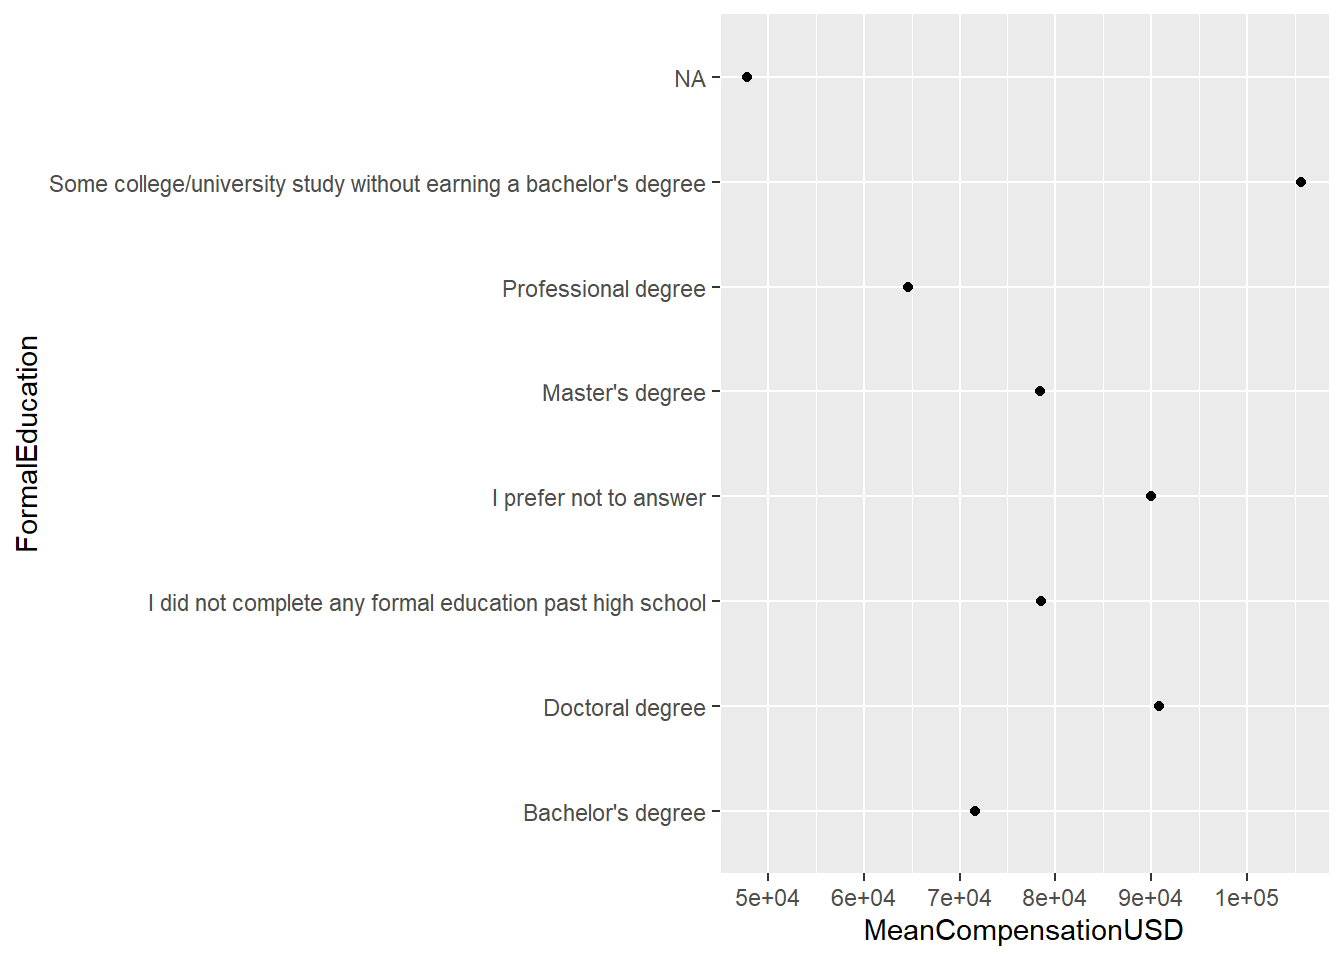
\includegraphics{bookdown-demo_files/figure-latex/unnamed-chunk-200-1.pdf}

Ta graf je sicer zelo informativen, ampak bi s težavo hitro ugotovili, kako so nivoji faktorja razvrščeni glede na plačo. ggplot razvrsti vrednosti glede na to, kako so razvrščene v faktorju:

\begin{Shaded}
\begin{Highlighting}[]
\FunctionTok{levels}\NormalTok{(ds\_jobs}\SpecialCharTok{$}\NormalTok{FormalEducation)}
\end{Highlighting}
\end{Shaded}

\begin{verbatim}
## [1] "Bachelor's degree"                                                
## [2] "Doctoral degree"                                                  
## [3] "I did not complete any formal education past high school"         
## [4] "I prefer not to answer"                                           
## [5] "Master's degree"                                                  
## [6] "Professional degree"                                              
## [7] "Some college/university study without earning a bachelor's degree"
\end{verbatim}

Morda bi bilo bolje tak graf urediti glede na vrednosti spremenljivke \texttt{MeanCompensationUSD}. Za to moramo določiti novo razvrstitev te spremenljivke. Za to obstaja v paketu \textbf{forcats}, ki je del tidyverse, funkcija \texttt{fct\_reorder()}.

\begin{Shaded}
\begin{Highlighting}[]
\FunctionTok{ggplot}\NormalTok{(ds\_jobs\_agg, }\FunctionTok{aes}\NormalTok{(}\AttributeTok{x =} \FunctionTok{fct\_reorder}\NormalTok{(FormalEducation, MeanCompensationUSD), }\AttributeTok{y =}\NormalTok{ MeanCompensationUSD)) }\SpecialCharTok{+}
  \FunctionTok{geom\_point}\NormalTok{() }\SpecialCharTok{+}
  \FunctionTok{coord\_flip}\NormalTok{()}
\end{Highlighting}
\end{Shaded}

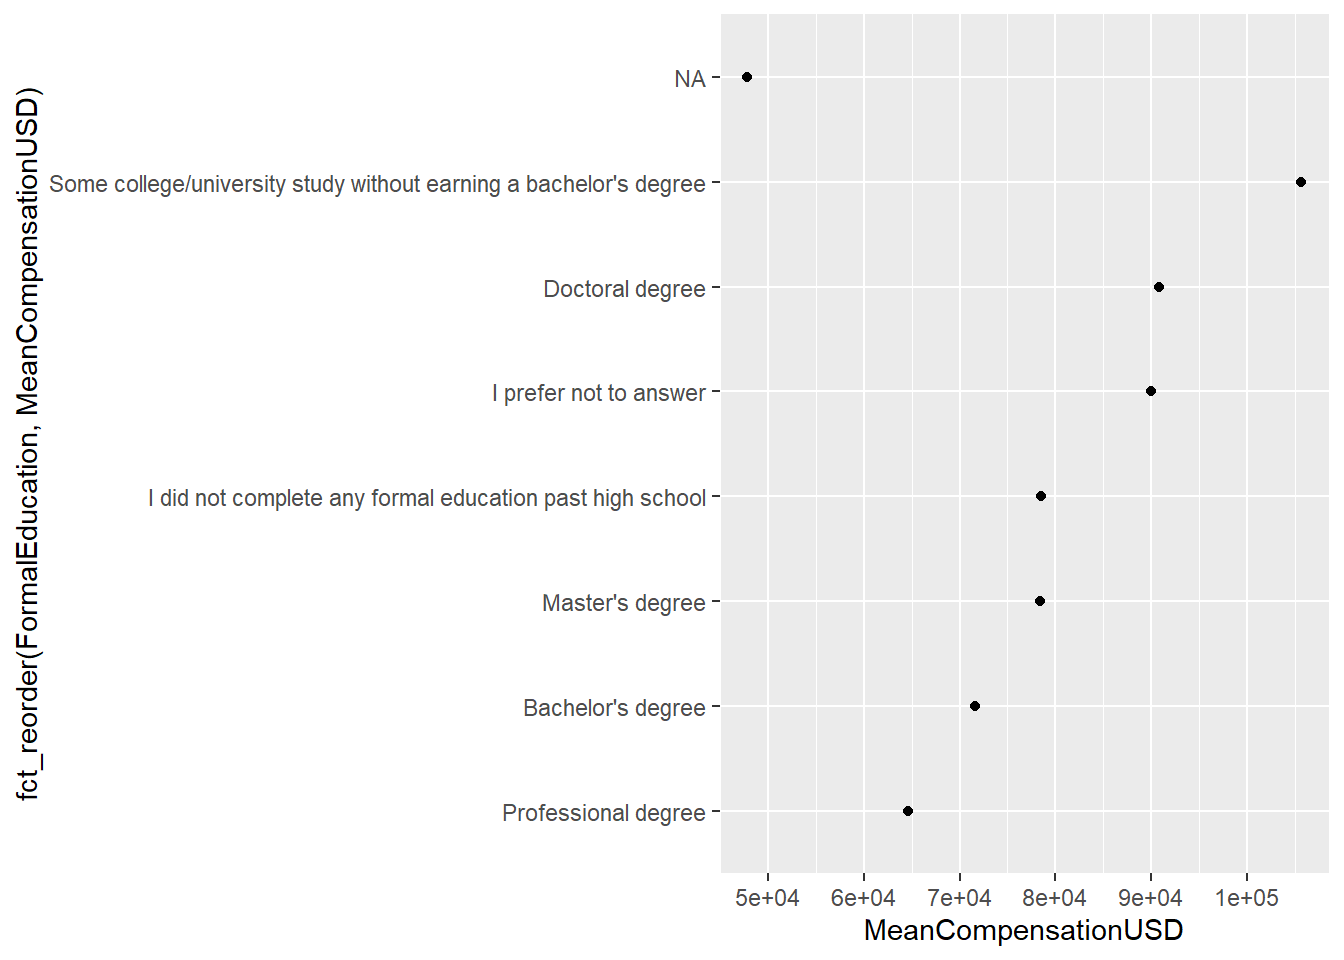
\includegraphics{bookdown-demo_files/figure-latex/unnamed-chunk-202-1.pdf}

Razvrstitev lahko uredimo tudi ročno s funkicjo \texttt{fct\_relevel()}, ki ohrani privzeto razvrstitev s tem, da podane nivoje premakne na začetek, oziroma lahko podamo arguemnt after.

\begin{Shaded}
\begin{Highlighting}[]
\FunctionTok{ggplot}\NormalTok{(ds\_jobs\_agg, }\FunctionTok{aes}\NormalTok{(}\AttributeTok{x =} \FunctionTok{fct\_relevel}\NormalTok{(FormalEducation, }\StringTok{"I prefer not to answer"}\NormalTok{, }\StringTok{"I did not complete any formal education past high school"}\NormalTok{, }\AttributeTok{after =} \DecValTok{0}\NormalTok{), }\AttributeTok{y =}\NormalTok{ MeanCompensationUSD)) }\SpecialCharTok{+}
  \FunctionTok{geom\_point}\NormalTok{() }\SpecialCharTok{+}
  \FunctionTok{coord\_flip}\NormalTok{()}
\end{Highlighting}
\end{Shaded}

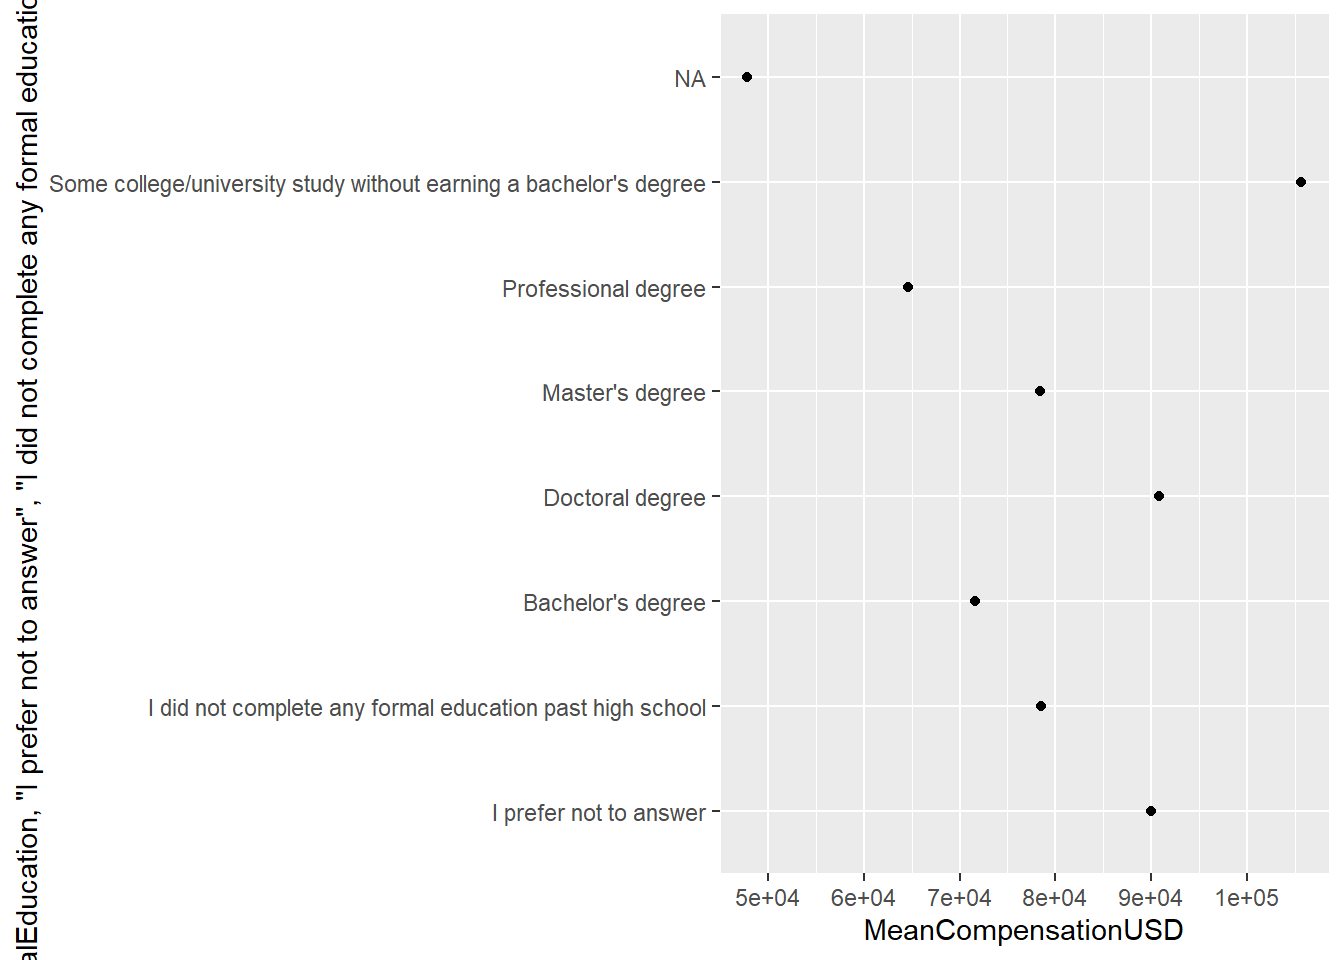
\includegraphics{bookdown-demo_files/figure-latex/unnamed-chunk-203-1.pdf}

\hypertarget{preimenivanje-obstojeux10dih-in-doloux10danje-novih-nivojev}{%
\subsection{Preimenivanje obstoječih in določanje novih nivojev}\label{preimenivanje-obstojeux10dih-in-doloux10danje-novih-nivojev}}

Nivoje faktorjev lahko preimenujemo s funkcijo \texttt{fct\_recode()}.

\begin{Shaded}
\begin{Highlighting}[]
\NormalTok{ds\_jobs }\OtherTok{\textless{}{-}}\NormalTok{ ds\_jobs }\SpecialCharTok{\%\textgreater{}\%}
  \FunctionTok{mutate}\NormalTok{(}\AttributeTok{EmploymentStatus =} \FunctionTok{fct\_recode}\NormalTok{(EmploymentStatus,}
                                        \StringTok{"full{-}time"} \OtherTok{=} \StringTok{"Employed full{-}time"}\NormalTok{,}
                                        \StringTok{"part{-}time"} \OtherTok{=} \StringTok{"Employed part{-}time"}\NormalTok{,}
                                        \StringTok{"other"} \OtherTok{=} \StringTok{"Independent contractor, freelancer, or self{-}employed"}\NormalTok{))}
\FunctionTok{head}\NormalTok{(ds\_jobs}\SpecialCharTok{$}\NormalTok{EmploymentStatus)}
\end{Highlighting}
\end{Shaded}

\begin{verbatim}
## [1] full-time full-time full-time part-time full-time full-time
## Levels: full-time part-time other
\end{verbatim}

Sorodno lahko zgornjo funkcijo zamenjamo z \texttt{fct\_collapse()}, ki lahko združi več nivojev v enega.

\hypertarget{razbitje-numeriux10dne-spremenljivke-na-intervale}{%
\subsection{Razbitje numerične spremenljivke na intervale}\label{razbitje-numeriux10dne-spremenljivke-na-intervale}}

Pogosto želimo kakšno numerično spremenljivko segmentirati na določene intervale. Na primer, pri določanju avtomobilskih zavarovalnih premij lahko zavarovance segmentiramo glede na starost. V R za to uporabimo funkcijo \texttt{cut()}. Razdelimo spremenljivko \texttt{Age} na intervale, kjer bodo osebe razdeljene do 25 let, nad 25 in to 35 let, nad 35 do 50 let, in nad 50 let.

\begin{Shaded}
\begin{Highlighting}[]
\NormalTok{ds\_jobs }\OtherTok{\textless{}{-}}\NormalTok{ ds\_jobs }\SpecialCharTok{\%\textgreater{}\%}
  \FunctionTok{mutate}\NormalTok{(}\AttributeTok{AgeInterval =} \FunctionTok{cut}\NormalTok{(Age, }\AttributeTok{breaks =} \FunctionTok{c}\NormalTok{(}\DecValTok{0}\NormalTok{, }\DecValTok{25}\NormalTok{, }\DecValTok{35}\NormalTok{, }\DecValTok{50}\NormalTok{, }\DecValTok{100}\NormalTok{)))}
\NormalTok{ds\_jobs\_agg }\OtherTok{\textless{}{-}}\NormalTok{ ds\_jobs }\SpecialCharTok{\%\textgreater{}\%}
  \FunctionTok{group\_by}\NormalTok{(AgeInterval) }\SpecialCharTok{\%\textgreater{}\%}
  \FunctionTok{summarise}\NormalTok{(}\AttributeTok{CompensationByAge =} \FunctionTok{mean}\NormalTok{(CompensationUSD))}
\FunctionTok{ggplot}\NormalTok{(ds\_jobs\_agg, }\FunctionTok{aes}\NormalTok{(}\AttributeTok{x =}\NormalTok{ AgeInterval, }\AttributeTok{y =}\NormalTok{ CompensationByAge)) }\SpecialCharTok{+} \FunctionTok{geom\_point}\NormalTok{()}
\end{Highlighting}
\end{Shaded}

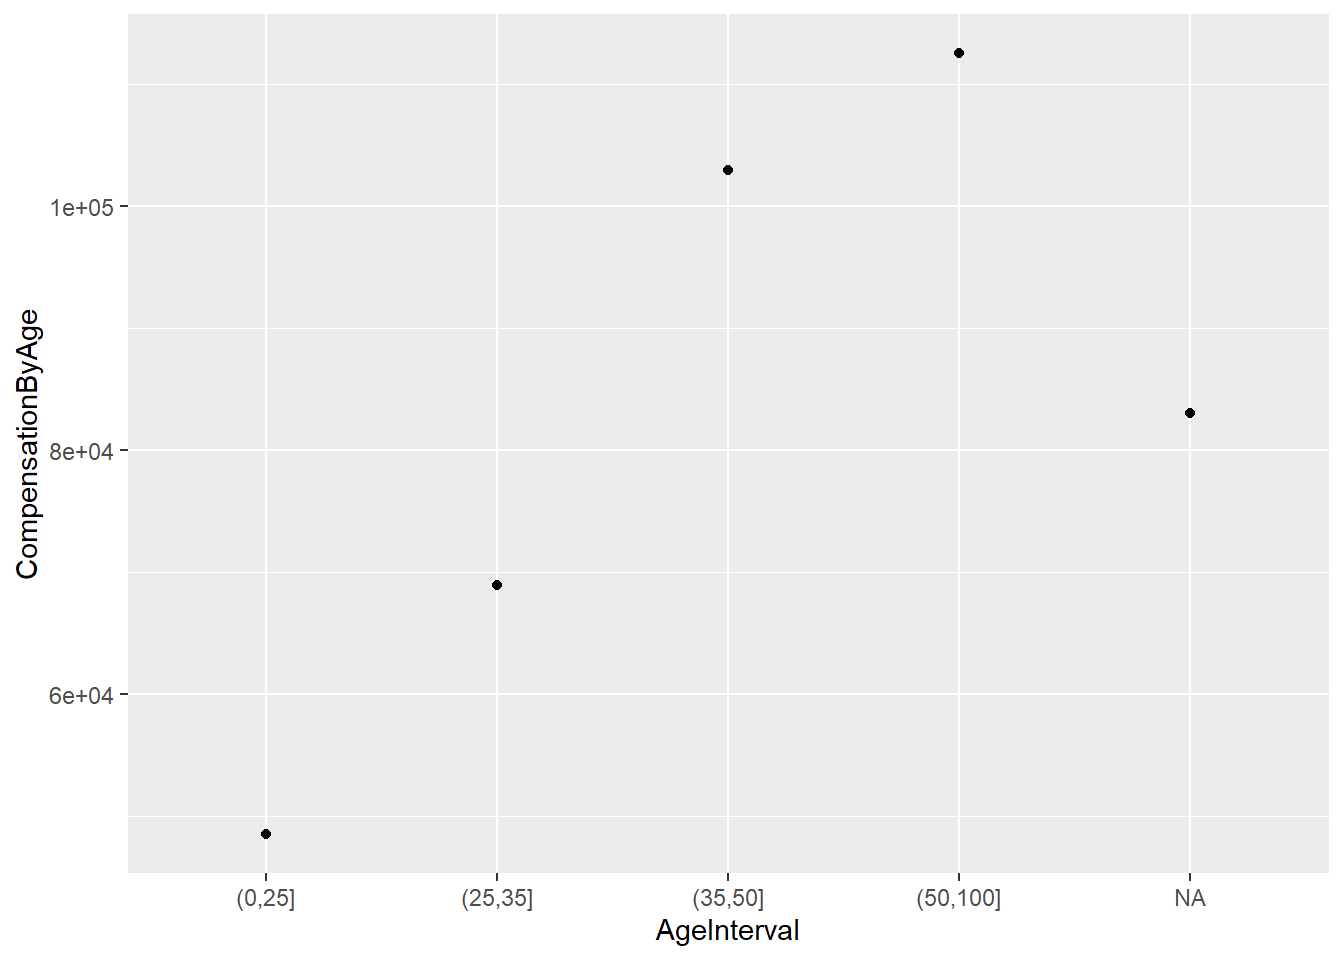
\includegraphics{bookdown-demo_files/figure-latex/unnamed-chunk-205-1.pdf}

\hypertarget{datumi-in-ure}{%
\section{Datumi in ure}\label{datumi-in-ure}}

Delo z datumi in urami morda na prvi pogled deluje precej enostavno. Vendar pa zaradi različnih fizikalnih zakonitosti ali človeških konstruktov lahko pride do težav. Na primer, vsako leto nima 365 dni. Prav tako v nekaterih časovnih conah 3. ura zjutraj ne sledi vedno 2. uri, saj pride do premika ure.

Za delo z datumi bomo uporabljali paket \textbf{lubridate}. Glavni komponenti v tem paketu sta \textbf{datum} (date) in \textbf{čas} (time), ter združena komponenta \textbf{datum in čas} (datetime). S tem paketom lahko datume ustvarimo na 2 načina:

\begin{enumerate}
\def\labelenumi{\arabic{enumi})}
\item
  Z nizom:

\begin{Shaded}
\begin{Highlighting}[]
\FunctionTok{library}\NormalTok{(lubridate)}
\FunctionTok{ymd}\NormalTok{(}\StringTok{"2021{-}04{-}02"}\NormalTok{)}
\end{Highlighting}
\end{Shaded}

\begin{verbatim}
## [1] "2021-04-02"
\end{verbatim}

\begin{Shaded}
\begin{Highlighting}[]
\FunctionTok{ymd}\NormalTok{(}\StringTok{"2021/04/02"}\NormalTok{)}
\end{Highlighting}
\end{Shaded}

\begin{verbatim}
## [1] "2021-04-02"
\end{verbatim}

\begin{Shaded}
\begin{Highlighting}[]
\FunctionTok{ymd}\NormalTok{(}\DecValTok{20210402}\NormalTok{)}
\end{Highlighting}
\end{Shaded}

\begin{verbatim}
## [1] "2021-04-02"
\end{verbatim}

\begin{Shaded}
\begin{Highlighting}[]
\FunctionTok{dmy}\NormalTok{(}\StringTok{"02.04.2021"}\NormalTok{)}
\end{Highlighting}
\end{Shaded}

\begin{verbatim}
## [1] "2021-04-02"
\end{verbatim}

\begin{Shaded}
\begin{Highlighting}[]
\FunctionTok{ymd\_hms}\NormalTok{(}\StringTok{"2021{-}04{-}02 12:01:00"}\NormalTok{) }\CommentTok{\# Tipa datetime.}
\end{Highlighting}
\end{Shaded}

\begin{verbatim}
## [1] "2021-04-02 12:01:00 UTC"
\end{verbatim}

\begin{Shaded}
\begin{Highlighting}[]
\FunctionTok{ymd}\NormalTok{(}\DecValTok{20210402}\NormalTok{, }\DecValTok{20210403}\NormalTok{)}
\end{Highlighting}
\end{Shaded}

\begin{verbatim}
## [1] "2021-04-02" "2021-04-03"
\end{verbatim}

\begin{Shaded}
\begin{Highlighting}[]
\FunctionTok{mdy}\NormalTok{(}\StringTok{"April 2nd, 2021"}\NormalTok{) }\CommentTok{\# Deluje za angleška imena mesecev}
\end{Highlighting}
\end{Shaded}

\begin{verbatim}
## [1] "2021-04-02"
\end{verbatim}
\item
  S posameznimi komponentami:

\begin{Shaded}
\begin{Highlighting}[]
\FunctionTok{make\_date}\NormalTok{(}\DecValTok{2021}\NormalTok{, }\DecValTok{4}\NormalTok{, }\DecValTok{2}\NormalTok{)}
\end{Highlighting}
\end{Shaded}

\begin{verbatim}
## [1] "2021-04-02"
\end{verbatim}

\begin{Shaded}
\begin{Highlighting}[]
\FunctionTok{make\_datetime}\NormalTok{(}\DecValTok{2021}\NormalTok{, }\DecValTok{4}\NormalTok{, }\DecValTok{2}\NormalTok{, }\DecValTok{12}\NormalTok{, }\DecValTok{1}\NormalTok{, }\DecValTok{0}\NormalTok{)}
\end{Highlighting}
\end{Shaded}

\begin{verbatim}
## [1] "2021-04-02 12:01:00 UTC"
\end{verbatim}
\end{enumerate}

Opazimo, da pri datumu in času spremenljivka hrani tudi informacijo o časovnem pasu. Privzeto lubridate dela s časovnim pasom UTC (Coordinated Universal Time), ki je naslednik GMT (Greenwich Mean Time). Prednost tega časovnega pasu je predvsem v tem, da se ne prilagaja spremembi ure v pomladnih in jesenskih mesecih. Te spremembe lahko privedejo do napak pri računanju z datumi in časi, tako da je računanje v UTC bolj varno. Seveda pa lahko ročno nastavimo drugi časovni pas z argumentom \texttt{tz}. Paket lubridate uporablja IANA časovne pasove (\url{https://www.iana.org/time-zones}), kateri so definirani s kombinacijo celine in države. Na primer, za Ljubljano bi časovni pas nastavili tako:

\begin{Shaded}
\begin{Highlighting}[]
\FunctionTok{ymd\_hms}\NormalTok{(}\StringTok{"2021{-}04{-}02 12:01:00"}\NormalTok{, }\AttributeTok{tz =} \StringTok{"Europe/Ljubljana"}\NormalTok{)}
\end{Highlighting}
\end{Shaded}

\begin{verbatim}
## [1] "2021-04-02 12:01:00 CEST"
\end{verbatim}

Pomembno je torej, da vemo, v katerem časovnem pasu so bile opravljene meritve v naših podatkih, da lahko potem ustrezno pretvorimo spremenljivko v časovno. Seveda pa lahko tudi pretvarjamo časovne spremenljivke med časovnimi pasovi. Za to uporabimo funkcijo \texttt{with\_tz()}. Vsakemu času v določenem časovnem pasu lahko priredimo nek čas v drugem časovnem pasu. V kolikor želimo bolj robustno računati z datumi in urami, potem lahko vedno datume pretvorimo v UTC čas, naredimo izračune in potem pretvorimo nazaj v lokalni časovni pas.

\begin{Shaded}
\begin{Highlighting}[]
\NormalTok{my\_datetime }\OtherTok{\textless{}{-}} \FunctionTok{ymd\_hms}\NormalTok{(}\StringTok{"2021{-}04{-}02 12:01:00"}\NormalTok{, }\AttributeTok{tz =} \StringTok{"Europe/Ljubljana"}\NormalTok{)}
\NormalTok{my\_datetime}
\end{Highlighting}
\end{Shaded}

\begin{verbatim}
## [1] "2021-04-02 12:01:00 CEST"
\end{verbatim}

\begin{Shaded}
\begin{Highlighting}[]
\NormalTok{my\_datetime\_UTC }\OtherTok{\textless{}{-}} \FunctionTok{with\_tz}\NormalTok{(my\_datetime, }\AttributeTok{tz =} \StringTok{"UTC"}\NormalTok{)}
\NormalTok{my\_datetime\_UTC}
\end{Highlighting}
\end{Shaded}

\begin{verbatim}
## [1] "2021-04-02 10:01:00 UTC"
\end{verbatim}

Hranita pa spremenljivki v ozadju isti čas. To lahko preverimo z:

\begin{Shaded}
\begin{Highlighting}[]
\NormalTok{my\_datetime }\SpecialCharTok{==}\NormalTok{ my\_datetime\_UTC}
\end{Highlighting}
\end{Shaded}

\begin{verbatim}
## [1] TRUE
\end{verbatim}

V R je časovni pas namenjen samo izpisu datumov in časov. Sama vrednost spremenljivke ostane nespremenjena. To lahko preverimo tako, da odštejemo en datum od drugega, kar nam vrne razliko v času:

\begin{Shaded}
\begin{Highlighting}[]
\NormalTok{my\_datetime }\SpecialCharTok{{-}}\NormalTok{ my\_datetime\_UTC}
\end{Highlighting}
\end{Shaded}

\begin{verbatim}
## Time difference of 0 secs
\end{verbatim}

V kolikor smo narobe prebrali datum v začetku (na primer, v podatkih je bil datum v UTC, prebrali pa smo v lokalnem času) zgornja pretvorba med časovnimi pasovi ni ustrezna, saj bomo s tem zajeli napačen čas. V tem primeru moramo uporabiti funkcijo \texttt{force\_tz()}. Predlagamo, da udeleženci sami poizkusijo, kaj naredi ta funkcija, tako da z njo pretvorijo \texttt{my\_datetime} v UTC in potem izračunajo razliko, podobno kot smo to naredili zgoraj.

Kadar delamo sekvence datumov in časov te upoštevajo premik ure in prehodov v naslednje dni. Poglejmo si prehod na poletni čas v letu 2021:

\begin{Shaded}
\begin{Highlighting}[]
\NormalTok{datetime\_dst }\OtherTok{\textless{}{-}} \FunctionTok{seq}\NormalTok{(}\FunctionTok{ymd\_hms}\NormalTok{(}\StringTok{"2021{-}03{-}28 00:00:00"}\NormalTok{, }\AttributeTok{tz =} \StringTok{"Europe/Ljubljana"}\NormalTok{), }
                    \FunctionTok{ymd\_hms}\NormalTok{(}\StringTok{"2021{-}03{-}28 04:00:00"}\NormalTok{, }\AttributeTok{tz =} \StringTok{"Europe/Ljubljana"}\NormalTok{), }
                    \AttributeTok{by =} \StringTok{"30 min"}\NormalTok{)}
\NormalTok{datetime\_dst}
\end{Highlighting}
\end{Shaded}

\begin{verbatim}
## [1] "2021-03-28 00:00:00 CET"  "2021-03-28 00:30:00 CET" 
## [3] "2021-03-28 01:00:00 CET"  "2021-03-28 01:30:00 CET" 
## [5] "2021-03-28 03:00:00 CEST" "2021-03-28 03:30:00 CEST"
## [7] "2021-03-28 04:00:00 CEST"
\end{verbatim}

\begin{Shaded}
\begin{Highlighting}[]
\FunctionTok{with\_tz}\NormalTok{(datetime\_dst, }\AttributeTok{tz =} \StringTok{"UTC"}\NormalTok{)}
\end{Highlighting}
\end{Shaded}

\begin{verbatim}
## [1] "2021-03-27 23:00:00 UTC" "2021-03-27 23:30:00 UTC"
## [3] "2021-03-28 00:00:00 UTC" "2021-03-28 00:30:00 UTC"
## [5] "2021-03-28 01:00:00 UTC" "2021-03-28 01:30:00 UTC"
## [7] "2021-03-28 02:00:00 UTC"
\end{verbatim}

Pozorni moramo biti tudi na kombiniranje datumov. V kolikor uporabimo funkcijo \texttt{c()}, vedno preverimo, v katerem časovnem pasu je rezultat.

\hypertarget{raux10dunanje-z-datumi-in-ux10dasi}{%
\subsection{Računanje z datumi in časi}\label{raux10dunanje-z-datumi-in-ux10dasi}}

Vsaka časovna spremenljivka, ki vsebuje datum in čas, je sestavljena iz komponent. Te so leto, mesec, dan, ura, minuta in sekunda. Za dostop do posameznih komponent imamo na voljo več funkcij:

\begin{itemize}
\tightlist
\item
  \texttt{year()}
\item
  \texttt{month()}
\item
  \texttt{mday()}. Dan v mesecu.
\item
  \texttt{wday()}. Dan v tednu. Privzeto se začne z nedeljo. To lahko spremenimo z argumentom \texttt{week\_start}.
\item
  \texttt{hour()}
\item
  \texttt{minute()}
\item
  \texttt{second()}
\end{itemize}

Poglejmo sedaj kaj vračajo te funkcije:

\begin{Shaded}
\begin{Highlighting}[]
\NormalTok{x }\OtherTok{\textless{}{-}} \FunctionTok{now}\NormalTok{()}
\NormalTok{x}
\end{Highlighting}
\end{Shaded}

\begin{verbatim}
## [1] "2021-06-11 17:26:16 CEST"
\end{verbatim}

\begin{Shaded}
\begin{Highlighting}[]
\FunctionTok{year}\NormalTok{(x)}
\end{Highlighting}
\end{Shaded}

\begin{verbatim}
## [1] 2021
\end{verbatim}

\begin{Shaded}
\begin{Highlighting}[]
\FunctionTok{month}\NormalTok{(x)}
\end{Highlighting}
\end{Shaded}

\begin{verbatim}
## [1] 6
\end{verbatim}

\begin{Shaded}
\begin{Highlighting}[]
\FunctionTok{mday}\NormalTok{(x)}
\end{Highlighting}
\end{Shaded}

\begin{verbatim}
## [1] 11
\end{verbatim}

\begin{Shaded}
\begin{Highlighting}[]
\FunctionTok{wday}\NormalTok{(x)}
\end{Highlighting}
\end{Shaded}

\begin{verbatim}
## [1] 6
\end{verbatim}

\begin{Shaded}
\begin{Highlighting}[]
\FunctionTok{wday}\NormalTok{(x, }\AttributeTok{week\_start =} \DecValTok{1}\NormalTok{)}
\end{Highlighting}
\end{Shaded}

\begin{verbatim}
## [1] 5
\end{verbatim}

\begin{Shaded}
\begin{Highlighting}[]
\FunctionTok{hour}\NormalTok{(x)}
\end{Highlighting}
\end{Shaded}

\begin{verbatim}
## [1] 17
\end{verbatim}

\begin{Shaded}
\begin{Highlighting}[]
\FunctionTok{minute}\NormalTok{(x)}
\end{Highlighting}
\end{Shaded}

\begin{verbatim}
## [1] 26
\end{verbatim}

\begin{Shaded}
\begin{Highlighting}[]
\FunctionTok{second}\NormalTok{(x)}
\end{Highlighting}
\end{Shaded}

\begin{verbatim}
## [1] 16.77942
\end{verbatim}

S komponentami lahko tudi spreminjamo dele časovne spremenljivke:

\begin{Shaded}
\begin{Highlighting}[]
\FunctionTok{mday}\NormalTok{(x) }\OtherTok{\textless{}{-}} \DecValTok{5}
\NormalTok{x}
\end{Highlighting}
\end{Shaded}

\begin{verbatim}
## [1] "2021-06-05 17:26:16 CEST"
\end{verbatim}

Pri računanju s časovnimi enotami v lubridate poznamo tri razrede:

\begin{itemize}
\tightlist
\item
  \textbf{trajanja} (ang. duration). Čas v sekundah. Funkcije \texttt{dseconds()}, \texttt{dminutes()}, \texttt{ddays()}, \texttt{dweeks()} in \texttt{dyears()}. Pri trajanjih se vedno uporabi pretvorba, da ima vsak dan 24 ur in vsako leto 365.25 dni. Slednje predstavlja povprečno šteilo dni v letu. Tako da bo funkcija \texttt{dyears(4)} vedno vrnila število sekund, ki ustreza 4x365.25 dnem, ki imajo vsak po 24 ur.
\item
  \textbf{periode} (ang. period). Čas v človeških enotah kot je na primer teden. Funkcije \texttt{seconds()}, \texttt{minutes()}, \texttt{days()}, \texttt{weeks()}, \texttt{months()} in \texttt{years()}.
\item
  \textbf{intervali} (ang. interval). Časovni interval med dvema točkama.
\end{itemize}

Pozoren bralec je morda opazil, da pri trajanjih nismo navedli funkcije za mesece. To je zaradi tega, ker imajo meseci lahko 28, 29, 30 ali 31 dni. Vsekakor bi pri izbiri osnovne enote za trajanja prišlo do neke arbitrarne odločitve, koliko dni vzamemo privzeto. 30 ali 31? V vsakem primeru bo vsaj polovica mesecev imela napačno trajanje. Pri dnevih in letih si lažje privoščimo posplošitev.

\begin{Shaded}
\begin{Highlighting}[]
\FunctionTok{ddays}\NormalTok{(}\DecValTok{1}\NormalTok{)}
\end{Highlighting}
\end{Shaded}

\begin{verbatim}
## [1] "86400s (~1 days)"
\end{verbatim}

\begin{Shaded}
\begin{Highlighting}[]
\FunctionTok{days}\NormalTok{(}\DecValTok{1}\NormalTok{)}
\end{Highlighting}
\end{Shaded}

\begin{verbatim}
## [1] "1d 0H 0M 0S"
\end{verbatim}

Poglejmo si preprost primer, kako dodati

\begin{Shaded}
\begin{Highlighting}[]
\NormalTok{my\_datetime }\OtherTok{\textless{}{-}} \FunctionTok{ymd\_hms}\NormalTok{(}\StringTok{"2021/06/08 11:05:30"}\NormalTok{, }\AttributeTok{tz =} \StringTok{"Europe/Ljubljana"}\NormalTok{)}
\NormalTok{my\_datetime }\SpecialCharTok{+} \FunctionTok{ddays}\NormalTok{(}\DecValTok{1}\NormalTok{)}
\end{Highlighting}
\end{Shaded}

\begin{verbatim}
## [1] "2021-06-09 11:05:30 CEST"
\end{verbatim}

\begin{Shaded}
\begin{Highlighting}[]
\NormalTok{my\_datetime }\SpecialCharTok{+} \FunctionTok{days}\NormalTok{(}\DecValTok{1}\NormalTok{)}
\end{Highlighting}
\end{Shaded}

\begin{verbatim}
## [1] "2021-06-09 11:05:30 CEST"
\end{verbatim}

\begin{Shaded}
\begin{Highlighting}[]
\NormalTok{my\_datetime }\SpecialCharTok{+} \FunctionTok{dminutes}\NormalTok{(}\DecValTok{120}\NormalTok{)}
\end{Highlighting}
\end{Shaded}

\begin{verbatim}
## [1] "2021-06-08 13:05:30 CEST"
\end{verbatim}

\begin{Shaded}
\begin{Highlighting}[]
\NormalTok{my\_datetime }\SpecialCharTok{+} \FunctionTok{minutes}\NormalTok{(}\DecValTok{120}\NormalTok{)}
\end{Highlighting}
\end{Shaded}

\begin{verbatim}
## [1] "2021-06-08 13:05:30 CEST"
\end{verbatim}

\begin{Shaded}
\begin{Highlighting}[]
\NormalTok{my\_datetime }\SpecialCharTok{+} \FunctionTok{months}\NormalTok{(}\DecValTok{2}\NormalTok{)}
\end{Highlighting}
\end{Shaded}

\begin{verbatim}
## [1] "2021-08-08 11:05:30 CEST"
\end{verbatim}

Trajanja in periode so si očitno zelo podobni ampak imajo eno veliko razliko, kadar računamo z dnevi, tedni in leti. Prvič, kadar bomo uporabljali \texttt{dyears()} lahko hitro pride do težave, saj bomo prišteli 0.25 dneva. Poglejmo si to na primeru:

\begin{Shaded}
\begin{Highlighting}[]
\NormalTok{my\_datetime }\SpecialCharTok{+} \FunctionTok{years}\NormalTok{(}\DecValTok{1}\NormalTok{)}
\end{Highlighting}
\end{Shaded}

\begin{verbatim}
## [1] "2022-06-08 11:05:30 CEST"
\end{verbatim}

\begin{Shaded}
\begin{Highlighting}[]
\NormalTok{my\_datetime }\SpecialCharTok{+} \FunctionTok{dyears}\NormalTok{(}\DecValTok{1}\NormalTok{)}
\end{Highlighting}
\end{Shaded}

\begin{verbatim}
## [1] "2022-06-08 17:05:30 CEST"
\end{verbatim}

Opazimo, da smo prišteli 6 dodatnih ur. Drugič, kaj se zgodi, kadar prištejemo teden ali dan v času, ko pride do premika ure. Premik ure se je po lokalnem času zgodil 28. 3. 2021 ob 2 zjutraj.

\begin{Shaded}
\begin{Highlighting}[]
\NormalTok{my\_datetime }\OtherTok{\textless{}{-}} \FunctionTok{ymd\_hms}\NormalTok{(}\StringTok{"2021/03/27 11:05:30"}\NormalTok{, }\AttributeTok{tz =} \StringTok{"Europe/Ljubljana"}\NormalTok{)}
\NormalTok{my\_datetime }\SpecialCharTok{+} \FunctionTok{ddays}\NormalTok{(}\DecValTok{1}\NormalTok{)}
\end{Highlighting}
\end{Shaded}

\begin{verbatim}
## [1] "2021-03-28 12:05:30 CEST"
\end{verbatim}

\begin{Shaded}
\begin{Highlighting}[]
\NormalTok{my\_datetime }\SpecialCharTok{+} \FunctionTok{days}\NormalTok{(}\DecValTok{1}\NormalTok{)}
\end{Highlighting}
\end{Shaded}

\begin{verbatim}
## [1] "2021-03-28 11:05:30 CEST"
\end{verbatim}

\begin{Shaded}
\begin{Highlighting}[]
\NormalTok{my\_datetime }\SpecialCharTok{+} \FunctionTok{dweeks}\NormalTok{(}\DecValTok{1}\NormalTok{)}
\end{Highlighting}
\end{Shaded}

\begin{verbatim}
## [1] "2021-04-03 12:05:30 CEST"
\end{verbatim}

\begin{Shaded}
\begin{Highlighting}[]
\NormalTok{my\_datetime }\SpecialCharTok{+} \FunctionTok{weeks}\NormalTok{(}\DecValTok{1}\NormalTok{)}
\end{Highlighting}
\end{Shaded}

\begin{verbatim}
## [1] "2021-04-03 11:05:30 CEST"
\end{verbatim}

Funkcija \texttt{years()} deluje kot bi pričakovali tudi na prestopnem letu:

\begin{Shaded}
\begin{Highlighting}[]
\NormalTok{my\_datetime }\OtherTok{\textless{}{-}} \FunctionTok{ymd\_hms}\NormalTok{(}\StringTok{"2020/06/08 11:05:30"}\NormalTok{, }\AttributeTok{tz =} \StringTok{"Europe/Ljubljana"}\NormalTok{)}
\NormalTok{my\_datetime }\SpecialCharTok{+} \FunctionTok{years}\NormalTok{(}\DecValTok{1}\NormalTok{)}
\end{Highlighting}
\end{Shaded}

\begin{verbatim}
## [1] "2021-06-08 11:05:30 CEST"
\end{verbatim}

S funkcijami trajanja in period lahko tudi računamo, na primer:

\begin{Shaded}
\begin{Highlighting}[]
\FunctionTok{dyears}\NormalTok{(}\DecValTok{2}\NormalTok{) }\SpecialCharTok{+} \FunctionTok{ddays}\NormalTok{(}\DecValTok{4}\NormalTok{) }\SpecialCharTok{+} \FunctionTok{dseconds}\NormalTok{(}\DecValTok{20}\NormalTok{)}
\end{Highlighting}
\end{Shaded}

\begin{verbatim}
## [1] "63460820s (~2.01 years)"
\end{verbatim}

\begin{Shaded}
\begin{Highlighting}[]
\FunctionTok{days}\NormalTok{(}\DecValTok{2}\NormalTok{) }\SpecialCharTok{+} \FunctionTok{minutes}\NormalTok{(}\DecValTok{20}\NormalTok{) }\SpecialCharTok{+} \FunctionTok{seconds}\NormalTok{(}\DecValTok{120}\NormalTok{)}
\end{Highlighting}
\end{Shaded}

\begin{verbatim}
## [1] "2d 0H 20M 120S"
\end{verbatim}

\begin{Shaded}
\begin{Highlighting}[]
\DecValTok{5} \SpecialCharTok{*} \FunctionTok{dminutes}\NormalTok{(}\DecValTok{20}\NormalTok{)}
\end{Highlighting}
\end{Shaded}

\begin{verbatim}
## [1] "6000s (~1.67 hours)"
\end{verbatim}

\begin{Shaded}
\begin{Highlighting}[]
\DecValTok{5} \SpecialCharTok{*} \FunctionTok{minutes}\NormalTok{(}\DecValTok{20}\NormalTok{)}
\end{Highlighting}
\end{Shaded}

\begin{verbatim}
## [1] "100M 0S"
\end{verbatim}

Najbolje, da jo prikažemo na dveh primerih -- premik ure in prestopno leto. Periode so bolj naraven prikaz za človeka.

\begin{Shaded}
\begin{Highlighting}[]
\NormalTok{my\_datetime }\OtherTok{\textless{}{-}} \FunctionTok{ymd\_hms}\NormalTok{(}\StringTok{"2021/06/08 11:05:30"}\NormalTok{, }\AttributeTok{tz =} \StringTok{"Europe/Ljubljana"}\NormalTok{)}
\NormalTok{my\_datetime }\SpecialCharTok{+} \FunctionTok{ddays}\NormalTok{(}\DecValTok{1}\NormalTok{)}
\end{Highlighting}
\end{Shaded}

\begin{verbatim}
## [1] "2021-06-09 11:05:30 CEST"
\end{verbatim}

\begin{Shaded}
\begin{Highlighting}[]
\NormalTok{my\_datetime }\SpecialCharTok{+} \FunctionTok{days}\NormalTok{(}\DecValTok{1}\NormalTok{)}
\end{Highlighting}
\end{Shaded}

\begin{verbatim}
## [1] "2021-06-09 11:05:30 CEST"
\end{verbatim}

\begin{Shaded}
\begin{Highlighting}[]
\NormalTok{my\_datetime }\SpecialCharTok{+} \FunctionTok{dminutes}\NormalTok{(}\DecValTok{120}\NormalTok{)}
\end{Highlighting}
\end{Shaded}

\begin{verbatim}
## [1] "2021-06-08 13:05:30 CEST"
\end{verbatim}

\begin{Shaded}
\begin{Highlighting}[]
\NormalTok{my\_datetime }\SpecialCharTok{+} \FunctionTok{minutes}\NormalTok{(}\DecValTok{120}\NormalTok{)}
\end{Highlighting}
\end{Shaded}

\begin{verbatim}
## [1] "2021-06-08 13:05:30 CEST"
\end{verbatim}

\begin{Shaded}
\begin{Highlighting}[]
\NormalTok{my\_datetime }\SpecialCharTok{+} \FunctionTok{dyears}\NormalTok{(}\DecValTok{1}\NormalTok{)}
\end{Highlighting}
\end{Shaded}

\begin{verbatim}
## [1] "2022-06-08 17:05:30 CEST"
\end{verbatim}

\begin{Shaded}
\begin{Highlighting}[]
\NormalTok{my\_datetime }\SpecialCharTok{+} \FunctionTok{years}\NormalTok{(}\DecValTok{1}\NormalTok{)}
\end{Highlighting}
\end{Shaded}

\begin{verbatim}
## [1] "2022-06-08 11:05:30 CEST"
\end{verbatim}

\begin{Shaded}
\begin{Highlighting}[]
\NormalTok{my\_datetime }\SpecialCharTok{+} \FunctionTok{months}\NormalTok{(}\DecValTok{2}\NormalTok{)}
\end{Highlighting}
\end{Shaded}

\begin{verbatim}
## [1] "2021-08-08 11:05:30 CEST"
\end{verbatim}

V bazi letalskih letov posodobimo podatke, tako da izračunamo niz, ki predstavlja točen odhod letala.

\begin{Shaded}
\begin{Highlighting}[]
\FunctionTok{library}\NormalTok{(nycflights13)}
\FunctionTok{head}\NormalTok{(flights)}
\end{Highlighting}
\end{Shaded}

\begin{verbatim}
## # A tibble: 6 x 20
##      ID  year month   day dep_time sched_dep_time dep_delay arr_time
##   <int> <int> <int> <int>    <int>          <int>     <dbl>    <int>
## 1     1  2013     1     1      517            515         2      830
## 2     2  2013     1     1      533            529         4      850
## 3     3  2013     1     1      542            540         2      923
## 4     4  2013     1     1      544            545        -1     1004
## 5     5  2013     1     1      554            600        -6      812
## 6     6  2013     1     1      554            558        -4      740
## # ... with 12 more variables: sched_arr_time <int>, arr_delay <dbl>,
## #   carrier <chr>, flight <int>, tailnum <chr>, origin <chr>, dest <chr>,
## #   air_time <dbl>, distance <dbl>, hour <dbl>, minute <dbl>, time_hour <dttm>
\end{verbatim}

\begin{Shaded}
\begin{Highlighting}[]
\NormalTok{flights\_datetime }\OtherTok{\textless{}{-}}\NormalTok{ flights }\SpecialCharTok{\%\textgreater{}\%} \FunctionTok{select}\NormalTok{(year, month, day, hour, minute) }\SpecialCharTok{\%\textgreater{}\%}
  \FunctionTok{mutate}\NormalTok{(}\AttributeTok{DepartureTime =} \FunctionTok{make\_datetime}\NormalTok{(year, month, day, hour, minute))}
\NormalTok{flights\_datetime}
\end{Highlighting}
\end{Shaded}

\begin{verbatim}
## # A tibble: 336,776 x 6
##     year month   day  hour minute DepartureTime      
##    <int> <int> <int> <dbl>  <dbl> <dttm>             
##  1  2013     1     1     5     15 2013-01-01 05:15:00
##  2  2013     1     1     5     29 2013-01-01 05:29:00
##  3  2013     1     1     5     40 2013-01-01 05:40:00
##  4  2013     1     1     5     45 2013-01-01 05:45:00
##  5  2013     1     1     6      0 2013-01-01 06:00:00
##  6  2013     1     1     5     58 2013-01-01 05:58:00
##  7  2013     1     1     6      0 2013-01-01 06:00:00
##  8  2013     1     1     6      0 2013-01-01 06:00:00
##  9  2013     1     1     6      0 2013-01-01 06:00:00
## 10  2013     1     1     6      0 2013-01-01 06:00:00
## # ... with 336,766 more rows
\end{verbatim}

\begin{Shaded}
\begin{Highlighting}[]
\FunctionTok{head}\NormalTok{(flights\_datetime}\SpecialCharTok{$}\NormalTok{DepartureTime)}
\end{Highlighting}
\end{Shaded}

\begin{verbatim}
## [1] "2013-01-01 05:15:00 UTC" "2013-01-01 05:29:00 UTC"
## [3] "2013-01-01 05:40:00 UTC" "2013-01-01 05:45:00 UTC"
## [5] "2013-01-01 06:00:00 UTC" "2013-01-01 05:58:00 UTC"
\end{verbatim}

Ali opazimo kakšno težavo? datume smo prebrali v časovni coni UTC, so pa podani v lokalni časovni coni. Podatkov torej nismo pretvorili pravilno! Poizkusimo še enkrat:

\begin{Shaded}
\begin{Highlighting}[]
\NormalTok{flights\_datetime }\OtherTok{\textless{}{-}}\NormalTok{ flights }\SpecialCharTok{\%\textgreater{}\%} \FunctionTok{select}\NormalTok{(year, month, day, hour, minute) }\SpecialCharTok{\%\textgreater{}\%}
  \FunctionTok{mutate}\NormalTok{(}\AttributeTok{DepartureTime =} \FunctionTok{make\_datetime}\NormalTok{(year, month, day, hour, minute,}
                                       \AttributeTok{tz =} \StringTok{"America/New\_York"}\NormalTok{))}
\NormalTok{flights\_datetime}
\end{Highlighting}
\end{Shaded}

\begin{verbatim}
## # A tibble: 336,776 x 6
##     year month   day  hour minute DepartureTime      
##    <int> <int> <int> <dbl>  <dbl> <dttm>             
##  1  2013     1     1     5     15 2013-01-01 05:15:00
##  2  2013     1     1     5     29 2013-01-01 05:29:00
##  3  2013     1     1     5     40 2013-01-01 05:40:00
##  4  2013     1     1     5     45 2013-01-01 05:45:00
##  5  2013     1     1     6      0 2013-01-01 06:00:00
##  6  2013     1     1     5     58 2013-01-01 05:58:00
##  7  2013     1     1     6      0 2013-01-01 06:00:00
##  8  2013     1     1     6      0 2013-01-01 06:00:00
##  9  2013     1     1     6      0 2013-01-01 06:00:00
## 10  2013     1     1     6      0 2013-01-01 06:00:00
## # ... with 336,766 more rows
\end{verbatim}

\begin{Shaded}
\begin{Highlighting}[]
\FunctionTok{head}\NormalTok{(flights\_datetime}\SpecialCharTok{$}\NormalTok{DepartureTime)}
\end{Highlighting}
\end{Shaded}

\begin{verbatim}
## [1] "2013-01-01 05:15:00 EST" "2013-01-01 05:29:00 EST"
## [3] "2013-01-01 05:40:00 EST" "2013-01-01 05:45:00 EST"
## [5] "2013-01-01 06:00:00 EST" "2013-01-01 05:58:00 EST"
\end{verbatim}

\hypertarget{shranjevanje-in-branje-podatkov}{%
\section{Shranjevanje in branje podatkov}\label{shranjevanje-in-branje-podatkov}}

\hypertarget{delo-z-binarnimi-datotekami}{%
\subsection{Delo z binarnimi datotekami}\label{delo-z-binarnimi-datotekami}}

V programskem jeziku R lahko shranjujemo in nalagamo (v trenutno sejo R) spremenljivke kot binarne objekte na dva prevladujoča načina:

\begin{enumerate}
\def\labelenumi{\arabic{enumi})}
\tightlist
\item
  S kombinacijo funkcij \texttt{save()} in \texttt{load()}.
\item
  S kombinacijo funkcij \texttt{saveRDS()} in \texttt{readRDS()}.
\end{enumerate}

Pomembna razlika med prvim in drugim pristopom je, da lahko s prvim shranimo več spremenljivk naenkrat, z drugim pa samo eno. Na prvi pogled bi torej pričakovali, da je prvi pristop boljši, oziroma bolj zaželen. Ampak ima eno pomembno slabost, zaradi katere predlagamo uporabo drugega pristopa.

Funkcija \texttt{save()} shrani spremenljivke v trenutni seji R v datoteko s končnico \emph{rda} ali \emph{RData}. To naredi tako, da shrani tako vrednost spremenljivke kot tudi ime spremenljivke. To pomeni, da ko bomo takšno datoteko prebrali v novo sejo R, bomo ustvarili spremenljivke z enakimi imeni, kot smo jih shranili. Pri tem pa lahko pride do težav. Recimo, da imamo v trenutni seji R že nek nabor spremenljivk nato pa želimo vanjo prenesti še neke druge spremenljivke, ki smo jih pred časom shranili s funkcijo \texttt{save()} v datoteko saved-data.rda. Kaj se bo zgodilo, če bo katera od spremenljivk v naši trenutni seji imela enako ime kot ena od spremenljivk shranjenih v saved-data.rda? R bo enostavno to spremenljivko prepisal s spremenljivko, ki se je nahajala v tej rda datoteki. Takšen postopek dela je lahko torej nevaren, saj lahko \emph{nevede} izbrišemo obstoječe spremenljivke.

Predlagamo torej uporabo druge kombinacije, torej funkcij \texttt{saveRDS()} in \texttt{readRDS()}. Funkcija \texttt{saveRDS()} shrani samo vrednost spremenljivke, ne pa tudi njenega imena, tako da ne pride do podobnih težav kot pri prvem pristopu. Končnica tako shranjenih datotek je \emph{rds}. Poglejmo si uporabo teh funkcij.

\begin{Shaded}
\begin{Highlighting}[]
\NormalTok{x }\OtherTok{\textless{}{-}} \FunctionTok{c}\NormalTok{(}\DecValTok{3}\NormalTok{, }\DecValTok{6}\NormalTok{, }\DecValTok{3}\NormalTok{, }\DecValTok{7}\NormalTok{)}
\NormalTok{x}
\end{Highlighting}
\end{Shaded}

\begin{verbatim}
## [1] 3 6 3 7
\end{verbatim}

\begin{Shaded}
\begin{Highlighting}[]
\FunctionTok{saveRDS}\NormalTok{(x, }\StringTok{"./my{-}saved{-}files/my{-}x.rds"}\NormalTok{)}

\NormalTok{x2 }\OtherTok{\textless{}{-}} \FunctionTok{readRDS}\NormalTok{(}\StringTok{"./my{-}saved{-}files/my{-}x.rds"}\NormalTok{)}
\NormalTok{x2}
\end{Highlighting}
\end{Shaded}

\begin{verbatim}
## [1] 3 6 3 7
\end{verbatim}

Vedno ko preberemo podatke v sejo R s funkcijo \texttt{readRDS()} ji moramo prirediti ime, saj je v rds datoteki shrnajena samo njena vrednost. S tem se tudi izognemo podobnim težavam kot pri funkcijah \texttt{save()} in \texttt{load()}.

Pomanjkljivost shranjevanja rds datotek pa je v tem, da lahko naenkrat shranimo samo 1 spremenljivko. Ampak to pomanjkljivost lahko zaobidemo, tako da več spremenljivk enostavno shranimov v seznam (\texttt{list()}). Poglejmo si sedaj na primer, kako bi shranili več spremenljivk.

\begin{Shaded}
\begin{Highlighting}[]
\NormalTok{tmp\_list }\OtherTok{\textless{}{-}} \FunctionTok{list}\NormalTok{(}
  \StringTok{"x"} \OtherTok{=}\NormalTok{ x,}
  \StringTok{"some\_datetime"} \OtherTok{=}\NormalTok{ my\_datetime,}
  \StringTok{"ds\_jobs"} \OtherTok{=}\NormalTok{ ds\_jobs}
\NormalTok{)}

\FunctionTok{saveRDS}\NormalTok{(tmp\_list, }\StringTok{"./my{-}saved{-}files/my{-}list.rds"}\NormalTok{)}
\NormalTok{read\_list }\OtherTok{\textless{}{-}} \FunctionTok{readRDS}\NormalTok{(}\StringTok{"./my{-}saved{-}files/my{-}list.rds"}\NormalTok{)}
\FunctionTok{names}\NormalTok{(read\_list)}
\end{Highlighting}
\end{Shaded}

\begin{verbatim}
## [1] "x"             "some_datetime" "ds_jobs"
\end{verbatim}

\begin{Shaded}
\begin{Highlighting}[]
\NormalTok{x2 }\OtherTok{\textless{}{-}}\NormalTok{ read\_list[[}\StringTok{"x"}\NormalTok{]]}
\NormalTok{x2}
\end{Highlighting}
\end{Shaded}

\begin{verbatim}
## [1] 3 6 3 7
\end{verbatim}

\begin{Shaded}
\begin{Highlighting}[]
\NormalTok{my\_datetime2 }\OtherTok{\textless{}{-}}\NormalTok{ read\_list[[}\StringTok{"some\_datetime"}\NormalTok{]]}
\NormalTok{my\_datetime2}
\end{Highlighting}
\end{Shaded}

\begin{verbatim}
## [1] "2021-06-08 11:05:30 CEST"
\end{verbatim}

\begin{Shaded}
\begin{Highlighting}[]
\NormalTok{ds\_jobs2 }\OtherTok{\textless{}{-}}\NormalTok{ read\_list[[}\StringTok{"ds\_jobs"}\NormalTok{]]}
\NormalTok{ds\_jobs2}
\end{Highlighting}
\end{Shaded}

\begin{verbatim}
## # A tibble: 3,186 x 8
##    Country    Age EmploymentStatus FormalEducation CompensationAmo~ ExchangeRate
##    <fct>    <dbl> <fct>            <fct>                      <dbl>        <dbl>
##  1 Austral~    43 full-time        Bachelor's deg~            80000     0.802   
##  2 Russia      33 full-time        Bachelor's deg~          1200000     0.0174  
##  3 Taiwan      26 full-time        Master's degree          1100000     0.0333  
##  4 United ~    25 part-time        Bachelor's deg~            20000     1       
##  5 United ~    33 full-time        Doctoral degree           100000     1       
##  6 Russia      22 full-time        Bachelor's deg~           624000     0.0174  
##  7 Colombia    34 full-time        Master's degree        156000000     0.000342
##  8 Germany     41 other            I did not comp~           150000     1.20    
##  9 Poland      29 full-time        Master's degree           126000     0.281   
## 10 United ~    35 full-time        Doctoral degree           133000     1       
## # ... with 3,176 more rows, and 2 more variables: CompensationUSD <dbl>,
## #   AgeInterval <fct>
\end{verbatim}

\hypertarget{branje-in-shranjevanje-z-ostalimi-datotekami}{%
\subsection{Branje in shranjevanje z ostalimi datotekami}\label{branje-in-shranjevanje-z-ostalimi-datotekami}}

\hypertarget{excel}{%
\subsubsection{Excel}\label{excel}}

Paket \textbf{openxlsx} omogoča delo z exelovimi razpredelnicami. Poglejmo si preproste a uporabne ukaze. Za branje podatkov s tem paketom uprabljamo \texttt{read.xlsx()}, za shranjevanje datotek pa \texttt{write.xlsx()}.

Preberimo podatke ocen, ki smo jih imeli tudi v testni skripti in jo pretvorimo v tibble:

\begin{Shaded}
\begin{Highlighting}[]
\FunctionTok{library}\NormalTok{(openxlsx)}
\NormalTok{ocene }\OtherTok{\textless{}{-}} \FunctionTok{tibble}\NormalTok{(openxlsx}\SpecialCharTok{::}\FunctionTok{read.xlsx}\NormalTok{(}\StringTok{"./test{-}script/data{-}raw/student{-}performance.xlsx"}\NormalTok{))}
\NormalTok{ocene}
\end{Highlighting}
\end{Shaded}

\begin{verbatim}
## # A tibble: 649 x 12
##    school sex   famsize Pstatus traveltime studytime internet absences    G1
##    <chr>  <chr> <chr>   <chr>        <dbl>     <dbl> <chr>       <dbl> <dbl>
##  1 GP     F     GT3     A                2         2 no              4     0
##  2 GP     F     GT3     T                1         2 yes             2     9
##  3 GP     F     LE3     T                1         2 yes             6    12
##  4 GP     F     GT3     T                1         3 yes             0    14
##  5 GP     F     GT3     T                1         2 no              0    11
##  6 GP     M     LE3     T                1         2 yes             6    12
##  7 GP     M     LE3     T                1         2 yes             0    13
##  8 GP     F     GT3     A                2         2 no              2    10
##  9 GP     M     LE3     A                1         2 yes             0    15
## 10 GP     M     GT3     T                1         2 yes             0    12
## # ... with 639 more rows, and 3 more variables: G2 <dbl>, G3 <dbl>,
## #   averageScore <dbl>
\end{verbatim}

Privzeto funkcija \texttt{read.xlsx()} odpre prvi list v datoteki in poišče glavo razpredelnice, če želimo druge liste moramo podati ime lista ali številko lista s parametrom \texttt{sheet}.

\begin{Shaded}
\begin{Highlighting}[]
\FunctionTok{library}\NormalTok{(openxlsx)}
\NormalTok{ocene\_portugalscina }\OtherTok{\textless{}{-}} \FunctionTok{tibble}\NormalTok{(}\FunctionTok{read.xlsx}\NormalTok{(}\StringTok{"./test{-}script/data{-}raw/student{-}performance.xlsx"}\NormalTok{, }\AttributeTok{sheet =} \DecValTok{1}\NormalTok{))}
\NormalTok{ocene\_matematika }\OtherTok{\textless{}{-}} \FunctionTok{tibble}\NormalTok{(}\FunctionTok{read.xlsx}\NormalTok{(}\StringTok{"./test{-}script/data{-}raw/student{-}performance.xlsx"}\NormalTok{, }\AttributeTok{sheet =} \StringTok{"Math scores"}\NormalTok{))}
\NormalTok{ocene\_portugalscina }\SpecialCharTok{\%\textgreater{}\%} 
  \FunctionTok{select}\NormalTok{(school, G1, G2, G3, averageScore)}
\end{Highlighting}
\end{Shaded}

\begin{verbatim}
## # A tibble: 649 x 5
##    school    G1    G2    G3 averageScore
##    <chr>  <dbl> <dbl> <dbl>        <dbl>
##  1 GP         0    11    11         7.33
##  2 GP         9    11    11        10.3 
##  3 GP        12    13    12        12.3 
##  4 GP        14    14    14        14   
##  5 GP        11    13    13        12.3 
##  6 GP        12    12    13        12.3 
##  7 GP        13    12    13        12.7 
##  8 GP        10    13    13        12   
##  9 GP        15    16    17        16   
## 10 GP        12    12    13        12.3 
## # ... with 639 more rows
\end{verbatim}

\begin{Shaded}
\begin{Highlighting}[]
\NormalTok{ocene\_matematika }\SpecialCharTok{\%\textgreater{}\%}
  \FunctionTok{select}\NormalTok{(school, G1, G2, G3, averageScore)}
\end{Highlighting}
\end{Shaded}

\begin{verbatim}
## # A tibble: 395 x 5
##    school    G1    G2    G3 averageScore
##    <chr>  <dbl> <dbl> <dbl>        <dbl>
##  1 GP         5     6     6         5.67
##  2 GP         5     5     6         5.33
##  3 GP         7     8    10         8.33
##  4 GP        15    14    15        14.7 
##  5 GP         6    10    10         8.67
##  6 GP        15    15    15        15   
##  7 GP        12    12    11        11.7 
##  8 GP         6     5     6         5.67
##  9 GP        16    18    19        17.7 
## 10 GP        14    15    15        14.7 
## # ... with 385 more rows
\end{verbatim}

Če ima datoteka veliko število listov jih lahko shranite v R-jev seznam (list).

\begin{Shaded}
\begin{Highlighting}[]
\FunctionTok{library}\NormalTok{(openxlsx)}
\NormalTok{path }\OtherTok{\textless{}{-}} \StringTok{"./test{-}script/data{-}raw/student{-}performance.xlsx"}
\NormalTok{imenaListov }\OtherTok{\textless{}{-}} \FunctionTok{getSheetNames}\NormalTok{(path)}
\NormalTok{ocene\_s }\OtherTok{\textless{}{-}} \FunctionTok{list}\NormalTok{()}
\ControlFlowTok{for}\NormalTok{(i }\ControlFlowTok{in} \DecValTok{1}\SpecialCharTok{:}\FunctionTok{length}\NormalTok{(imenaListov)) \{}
\NormalTok{  ocene\_s[[i]] }\OtherTok{\textless{}{-}} \FunctionTok{tibble}\NormalTok{(}\FunctionTok{read.xlsx}\NormalTok{(path))}
\NormalTok{\}}
\NormalTok{ocene\_s}
\end{Highlighting}
\end{Shaded}

\begin{verbatim}
## [[1]]
## # A tibble: 649 x 12
##    school sex   famsize Pstatus traveltime studytime internet absences    G1
##    <chr>  <chr> <chr>   <chr>        <dbl>     <dbl> <chr>       <dbl> <dbl>
##  1 GP     F     GT3     A                2         2 no              4     0
##  2 GP     F     GT3     T                1         2 yes             2     9
##  3 GP     F     LE3     T                1         2 yes             6    12
##  4 GP     F     GT3     T                1         3 yes             0    14
##  5 GP     F     GT3     T                1         2 no              0    11
##  6 GP     M     LE3     T                1         2 yes             6    12
##  7 GP     M     LE3     T                1         2 yes             0    13
##  8 GP     F     GT3     A                2         2 no              2    10
##  9 GP     M     LE3     A                1         2 yes             0    15
## 10 GP     M     GT3     T                1         2 yes             0    12
## # ... with 639 more rows, and 3 more variables: G2 <dbl>, G3 <dbl>,
## #   averageScore <dbl>
## 
## [[2]]
## # A tibble: 649 x 12
##    school sex   famsize Pstatus traveltime studytime internet absences    G1
##    <chr>  <chr> <chr>   <chr>        <dbl>     <dbl> <chr>       <dbl> <dbl>
##  1 GP     F     GT3     A                2         2 no              4     0
##  2 GP     F     GT3     T                1         2 yes             2     9
##  3 GP     F     LE3     T                1         2 yes             6    12
##  4 GP     F     GT3     T                1         3 yes             0    14
##  5 GP     F     GT3     T                1         2 no              0    11
##  6 GP     M     LE3     T                1         2 yes             6    12
##  7 GP     M     LE3     T                1         2 yes             0    13
##  8 GP     F     GT3     A                2         2 no              2    10
##  9 GP     M     LE3     A                1         2 yes             0    15
## 10 GP     M     GT3     T                1         2 yes             0    12
## # ... with 639 more rows, and 3 more variables: G2 <dbl>, G3 <dbl>,
## #   averageScore <dbl>
\end{verbatim}

V primeru, da je razpredelnica v excelovem listu premaknjena ali pa želimo prebrati le del podatkov, lahko uporabimo parametra \texttt{startRow} in \texttt{cols}. Preberimo samo ocene za matematiko brez ostalih vrednosti.

\begin{Shaded}
\begin{Highlighting}[]
\NormalTok{path }\OtherTok{\textless{}{-}} \StringTok{"./test{-}script/data{-}raw/student{-}performance.xlsx"}
\NormalTok{ocene\_math }\OtherTok{\textless{}{-}} \FunctionTok{tibble}\NormalTok{(}\FunctionTok{read.xlsx}\NormalTok{(path, }\AttributeTok{sheet =} \StringTok{"Math scores"}\NormalTok{, }\AttributeTok{startRow =} \DecValTok{1}\NormalTok{, }
                               \AttributeTok{cols =} \DecValTok{9}\SpecialCharTok{:}\DecValTok{12}\NormalTok{))}
\NormalTok{ocene\_math}
\end{Highlighting}
\end{Shaded}

\begin{verbatim}
## # A tibble: 395 x 4
##       G1    G2    G3 averageScore
##    <dbl> <dbl> <dbl>        <dbl>
##  1     5     6     6         5.67
##  2     5     5     6         5.33
##  3     7     8    10         8.33
##  4    15    14    15        14.7 
##  5     6    10    10         8.67
##  6    15    15    15        15   
##  7    12    12    11        11.7 
##  8     6     5     6         5.67
##  9    16    18    19        17.7 
## 10    14    15    15        14.7 
## # ... with 385 more rows
\end{verbatim}

Da podatke shranimo na disk uporabimo \texttt{write.xlsx()}.

\begin{Shaded}
\begin{Highlighting}[]
\NormalTok{path }\OtherTok{\textless{}{-}} \StringTok{"./test{-}script/data{-}raw/samo{-}ocene{-}math.xlsx"}
\FunctionTok{write.xlsx}\NormalTok{(ocene\_math, path)}
\end{Highlighting}
\end{Shaded}

\hypertarget{spss}{%
\subsubsection{SPSS}\label{spss}}

SPSS je program za statistično analizo. Datoteke povezane z SPSS imajo običajno končnico \emph{.sav}. Za branje iz in uvažanje v SPSS lahko uporabimo paket \textbf{haven}. V mapi \emph{data\_raw} imamo podatke o osebah \emph{osebe.sav}. Za uvoz teh podatkov v R uporabimo funkcijo \texttt{read\_sav}.

\begin{Shaded}
\begin{Highlighting}[]
\FunctionTok{library}\NormalTok{(haven)}
\NormalTok{podatki }\OtherTok{\textless{}{-}} \FunctionTok{read\_sav}\NormalTok{(}\StringTok{"./data{-}raw/osebe.sav"}\NormalTok{)}
\NormalTok{podatki}
\end{Highlighting}
\end{Shaded}

\begin{verbatim}
## # A tibble: 5 x 5
##   Ime    Visina  Teza Spol  Starost
##   <chr>   <dbl> <dbl> <chr>   <dbl>
## 1 Alen      171    70 m          41
## 2 Bojan     185    78 m          35
## 3 Cvetka    165    64 z          28
## 4 Dejan     190    95 m          52
## 5 Eva       152    67 z          22
\end{verbatim}

Da shranimo data frame v sav datoteko, uporabimo funkcijo \texttt{write\_sav()}. Shranimo sedaj data frame \texttt{iris} v sav datoteko:

\begin{Shaded}
\begin{Highlighting}[]
\FunctionTok{write\_sav}\NormalTok{(iris, }\StringTok{"./data{-}clean/iris.sav"}\NormalTok{)}
\end{Highlighting}
\end{Shaded}

\begin{verbatim}
## Error: Failed to open 'C:\Users\Gregor\Documents\shared_files\workshops\urejanje-podatkov\data-clean\iris.sav' for writing
\end{verbatim}

Paket haven ima tudi funkcijo \texttt{read\_por()} ki podpira starejše verzije datotek iz SPSS.

\hypertarget{ali-ux17eelite-izvedeti-veux10d-2}{%
\section{Ali želite izvedeti več?}\label{ali-ux17eelite-izvedeti-veux10d-2}}

V tem poglavju smo si ogledali operacije treh paketov tidyversa. Če želite hiter in dokaj celovit pregled nad vsemi ukazi priporočamo, da si za vsak paket ogledate tako imenovan \textbf{cheat sheet}:

\begin{itemize}
\tightlist
\item
  \textbf{stringr}: \url{https://evoldyn.gitlab.io/evomics-2018/ref-sheets/R_strings.pdf}
\item
  \textbf{forcats}: \url{http://www.flutterbys.com.au/stats/downloads/slides/figure/factors.pdf}
\item
  \textbf{lubridate}: \url{https://evoldyn.gitlab.io/evomics-2018/ref-sheets/R_lubridate.pdf}
\end{itemize}

Paket \textbf{stringr} uporablja paket \textbf{stringi}, ki ima na voljo 5x več operacij, ki pa niso tako pogosto uporabljene. Če se boste pri svojem delu srečali z zahtevnejšimi nalogami lahko uporabite ta paket.

Za razumevanje regularnih izrazov in tudi avtomatsko razlago priporočamo stran \url{https://regex101.com/}.

\hypertarget{domaux10da-naloga-2}{%
\section{Domača naloga}\label{domaux10da-naloga-2}}

\begin{enumerate}
\def\labelenumi{\arabic{enumi})}
\item
  Odprite prvi list ocen v \texttt{student-performance.xlsx} v mapi \texttt{test-script/data-raw/}.

  \begin{itemize}
  \tightlist
  \item
    Odprite le stolpce school, absences, G1, G2, G3 in averageScore.
  \item
    Dodajte stolpec \emph{točke}, ki ima vrednosti med 0 in 100, tako da ima najvišja pripadajoča vrednost v averageScore vrednost 100.
  \item
    Dodajte stolpec \emph{ocena}, kjer so vrednosti za \emph{točke} med 0 in 10 enake 1, 10 in 20 enake 2 itd.
  \item
    Dodajte stolpec \emph{besedna\_ocena} tipa faktor, ki bo imel vrednosti glede na \emph{oceno} in sicer ocene \textless6 = ``nezadostno'', 6 = ``zadostno'', 7 in 8 = ``dobro'', 9 = ``zelo dobro'' in 10 = ``odlično''.
  \end{itemize}

\begin{verbatim}
## # A tibble: 649 x 9
##    school absences    G1    G2    G3 averageScore točke ocena besedna_ocena
##    <chr>     <dbl> <dbl> <dbl> <dbl>        <dbl> <dbl> <dbl> <fct>        
##  1 GP            4     0    11    11         7.33  39.3     4 nezadostno   
##  2 GP            2     9    11    11        10.3   55.4     6 zadostno     
##  3 GP            6    12    13    12        12.3   66.1     7 dobro        
##  4 GP            0    14    14    14        14     75       8 dobro        
##  5 GP            0    11    13    13        12.3   66.1     7 dobro        
##  6 GP            6    12    12    13        12.3   66.1     7 dobro        
##  7 GP            0    13    12    13        12.7   67.9     7 dobro        
##  8 GP            2    10    13    13        12     64.3     7 dobro        
##  9 GP            0    15    16    17        16     85.7     9 zelo dobro   
## 10 GP            0    12    12    13        12.3   66.1     7 dobro        
## # ... with 639 more rows
\end{verbatim}
\item
  Naložite paket \texttt{nycflights13} s podatki letov. V tej bazi je več razpredelnic in sicer \textbf{flights}, \textbf{airlines}, \textbf{planes}, \textbf{airports} in \textbf{weather}. Za razumevanje si pomagajte z \texttt{?flights}.

  \begin{enumerate}
  \def\labelenumii{\alph{enumii})}
  \tightlist
  \item
    Izpišite vsa letališča, ki imajo 3 ali več besed v svojem imenu.
  \end{enumerate}

\begin{verbatim}
## # A tibble: 837 x 8
##    faa   name                        lat    lon   alt    tz dst   tzone         
##    <chr> <chr>                     <dbl>  <dbl> <dbl> <dbl> <chr> <chr>         
##  1 06A   Moton Field Municipal Ai~  32.5  -85.7   264    -6 A     America/Chica~
##  2 09J   Jekyll Island Airport      31.1  -81.4    11    -5 A     America/New_Y~
##  3 0A9   Elizabethton Municipal A~  36.4  -82.2  1593    -5 A     America/New_Y~
##  4 0G6   Williams County Airport    41.5  -84.5   730    -5 A     America/New_Y~
##  5 0G7   Finger Lakes Regional Ai~  42.9  -76.8   492    -5 A     America/New_Y~
##  6 0P2   Shoestring Aviation Airf~  39.8  -76.6  1000    -5 U     America/New_Y~
##  7 0S9   Jefferson County Intl      48.1 -123.    108    -8 A     America/Los_A~
##  8 0W3   Harford County Airport     39.6  -76.2   409    -5 A     America/New_Y~
##  9 10C   Galt Field Airport         42.4  -88.4   875    -6 U     America/Chica~
## 10 17G   Port Bucyrus-Crawford Co~  40.8  -83.0  1003    -5 A     America/New_Y~
## # ... with 827 more rows
\end{verbatim}

  \begin{enumerate}
  \def\labelenumii{\alph{enumii})}
  \setcounter{enumii}{1}
  \tightlist
  \item
    \textbf{Težja} Spremenite imena letališč tako, da odstranite besedi ``Airport'' ali ``Airfield'' iz konca imena.
  \end{enumerate}

\begin{verbatim}
## # A tibble: 1,458 x 8
##    faa   name                      lat    lon   alt    tz dst   tzone           
##    <chr> <chr>                   <dbl>  <dbl> <dbl> <dbl> <chr> <chr>           
##  1 04G   "Lansdowne "             41.1  -80.6  1044    -5 A     America/New_York
##  2 06A   "Moton Field Municipal~  32.5  -85.7   264    -6 A     America/Chicago 
##  3 06C   "Schaumburg Regional"    42.0  -88.1   801    -6 A     America/Chicago 
##  4 06N   "Randall "               41.4  -74.4   523    -5 A     America/New_York
##  5 09J   "Jekyll Island "         31.1  -81.4    11    -5 A     America/New_York
##  6 0A9   "Elizabethton Municipa~  36.4  -82.2  1593    -5 A     America/New_York
##  7 0G6   "Williams County "       41.5  -84.5   730    -5 A     America/New_York
##  8 0G7   "Finger Lakes Regional~  42.9  -76.8   492    -5 A     America/New_York
##  9 0P2   "Shoestring Aviation "   39.8  -76.6  1000    -5 U     America/New_York
## 10 0S9   "Jefferson County Intl"  48.1 -123.    108    -8 A     America/Los_Ang~
## # ... with 1,448 more rows
\end{verbatim}

  \begin{enumerate}
  \def\labelenumii{\alph{enumii})}
  \setcounter{enumii}{2}
  \tightlist
  \item
    \textbf{Daljša} Za vsak let sestavite besedno poročilo spodnje oblike, ki ga shranite v stolpec \textbf{Poročilo leta}.
  \end{enumerate}

  Besedilo naj se glasi: ``Let iz letalisca Newark Liberty Intl dne 22.01.13 ob 11:00 v letalisce George Bush Intercontinental je imel 2 minut zamude v odhodu in 11 v prihodu.''

  Minute so lahko tudi negativne.

\begin{verbatim}
## # A tibble: 336,776 x 2
##    `Poročilo leta`                                           dep_string         
##    <chr>                                                     <dttm>             
##  1 Let iz letalisca Newark Liberty Intl, dne 22.01.13, ob 1~ 2013-01-22 11:00:00
##  2 Let iz letalisca La Guardia, dne 23.01.13, ob 01:00 v le~ 2013-01-23 01:00:00
##  3 Let iz letalisca John F Kennedy Intl, dne 23.01.13, ob 1~ 2013-01-23 12:00:00
##  4 <NA>                                                      2013-01-23 17:00:00
##  5 Let iz letalisca La Guardia, dne 26.01.13, ob 00:00 v le~ 2013-01-26 00:00:00
##  6 Let iz letalisca Newark Liberty Intl, dne 24.01.13, ob 0~ 2013-01-24 06:00:00
##  7 Let iz letalisca Newark Liberty Intl, dne 26.01.13, ob 0~ 2013-01-26 00:00:00
##  8 Let iz letalisca La Guardia, dne 26.01.13, ob 00:00 v le~ 2013-01-26 00:00:00
##  9 Let iz letalisca John F Kennedy Intl, dne 26.01.13, ob 0~ 2013-01-26 00:00:00
## 10 Let iz letalisca La Guardia, dne 26.01.13, ob 00:00 v le~ 2013-01-26 00:00:00
## # ... with 336,766 more rows
\end{verbatim}
\end{enumerate}

  \bibliography{book.bib}

\end{document}
